\documentclass[twoside]{book}

% Packages required by doxygen
\usepackage{fixltx2e}
\usepackage{calc}
\usepackage{doxygen}
\usepackage[export]{adjustbox} % also loads graphicx
\usepackage{graphicx}
\usepackage[utf8]{inputenc}
\usepackage{makeidx}
\usepackage{multicol}
\usepackage{multirow}
\PassOptionsToPackage{warn}{textcomp}
\usepackage{textcomp}
\usepackage[nointegrals]{wasysym}
\usepackage[table]{xcolor}

% Font selection
\usepackage[T1]{fontenc}
\usepackage[scaled=.90]{helvet}
\usepackage{courier}
\usepackage{amssymb}
\usepackage{sectsty}
\renewcommand{\familydefault}{\sfdefault}
\allsectionsfont{%
  \fontseries{bc}\selectfont%
  \color{darkgray}%
}
\renewcommand{\DoxyLabelFont}{%
  \fontseries{bc}\selectfont%
  \color{darkgray}%
}
\newcommand{\+}{\discretionary{\mbox{\scriptsize$\hookleftarrow$}}{}{}}

% Page & text layout
\usepackage{geometry}
\geometry{%
  a4paper,%
  top=2.5cm,%
  bottom=2.5cm,%
  left=2.5cm,%
  right=2.5cm%
}
\tolerance=750
\hfuzz=15pt
\hbadness=750
\setlength{\emergencystretch}{15pt}
\setlength{\parindent}{0cm}
\setlength{\parskip}{3ex plus 2ex minus 2ex}
\makeatletter
\renewcommand{\paragraph}{%
  \@startsection{paragraph}{4}{0ex}{-1.0ex}{1.0ex}{%
    \normalfont\normalsize\bfseries\SS@parafont%
  }%
}
\renewcommand{\subparagraph}{%
  \@startsection{subparagraph}{5}{0ex}{-1.0ex}{1.0ex}{%
    \normalfont\normalsize\bfseries\SS@subparafont%
  }%
}
\makeatother

% Headers & footers
\usepackage{fancyhdr}
\pagestyle{fancyplain}
\fancyhead[LE]{\fancyplain{}{\bfseries\thepage}}
\fancyhead[CE]{\fancyplain{}{}}
\fancyhead[RE]{\fancyplain{}{\bfseries\leftmark}}
\fancyhead[LO]{\fancyplain{}{\bfseries\rightmark}}
\fancyhead[CO]{\fancyplain{}{}}
\fancyhead[RO]{\fancyplain{}{\bfseries\thepage}}
\fancyfoot[LE]{\fancyplain{}{}}
\fancyfoot[CE]{\fancyplain{}{}}
\fancyfoot[RE]{\fancyplain{}{\bfseries\scriptsize Generated by Doxygen }}
\fancyfoot[LO]{\fancyplain{}{\bfseries\scriptsize Generated by Doxygen }}
\fancyfoot[CO]{\fancyplain{}{}}
\fancyfoot[RO]{\fancyplain{}{}}
\renewcommand{\footrulewidth}{0.4pt}
\renewcommand{\chaptermark}[1]{%
  \markboth{#1}{}%
}
\renewcommand{\sectionmark}[1]{%
  \markright{\thesection\ #1}%
}

% Indices & bibliography
\usepackage{natbib}
\usepackage[titles]{tocloft}
\setcounter{tocdepth}{3}
\setcounter{secnumdepth}{5}
\makeindex

% Hyperlinks (required, but should be loaded last)
\usepackage{ifpdf}
\ifpdf
  \usepackage[pdftex,pagebackref=true]{hyperref}
\else
  \usepackage[ps2pdf,pagebackref=true]{hyperref}
\fi
\hypersetup{%
  colorlinks=true,%
  linkcolor=blue,%
  citecolor=blue,%
  unicode%
}

% Custom commands
\newcommand{\clearemptydoublepage}{%
  \newpage{\pagestyle{empty}\cleardoublepage}%
}

\usepackage{caption}
\captionsetup{labelsep=space,justification=centering,font={bf},singlelinecheck=off,skip=4pt,position=top}

%===== C O N T E N T S =====

\begin{document}

% Titlepage & ToC
\hypersetup{pageanchor=false,
             bookmarksnumbered=true,
             pdfencoding=unicode
            }
\pagenumbering{alph}
\begin{titlepage}
\vspace*{7cm}
\begin{center}%
{\Large Stor\+Trok \\[1ex]\large 1 }\\
\vspace*{1cm}
{\large Generated by Doxygen 1.8.13}\\
\end{center}
\end{titlepage}
\clearemptydoublepage
\pagenumbering{roman}
\tableofcontents
\clearemptydoublepage
\pagenumbering{arabic}
\hypersetup{pageanchor=true}

%--- Begin generated contents ---
\chapter{Hierarchical Index}
\section{Class Hierarchy}
This inheritance list is sorted roughly, but not completely, alphabetically\+:\begin{DoxyCompactList}
\item \contentsline{section}{Angle\+Range}{\pageref{class_angle_range}}{}
\item \contentsline{section}{Explosion\+Point}{\pageref{struct_explosion_point}}{}
\item \contentsline{section}{Full\+Mission}{\pageref{class_full_mission}}{}
\item \contentsline{section}{Game\+Preferences}{\pageref{class_game_preferences}}{}
\item \contentsline{section}{Interactive\+Message\+Button}{\pageref{class_interactive_message_button}}{}
\item \contentsline{section}{Inventar}{\pageref{class_inventar}}{}
\item \contentsline{section}{Mission\+Enemy}{\pageref{class_mission_enemy}}{}
\item \contentsline{section}{Mission\+Goal}{\pageref{class_mission_goal}}{}
\item \contentsline{section}{Mission\+Part}{\pageref{class_mission_part}}{}
\item Mono\+Behaviour\begin{DoxyCompactList}
\item \contentsline{section}{Alarm\+UI}{\pageref{class_alarm_u_i}}{}
\item \contentsline{section}{Asteroid}{\pageref{class_asteroid}}{}
\item \contentsline{section}{Audio\+Assets}{\pageref{class_audio_assets}}{}
\item \contentsline{section}{Auspuff}{\pageref{class_auspuff}}{}
\item \contentsline{section}{Bezier\+Curve}{\pageref{class_bezier_curve}}{}
\item \contentsline{section}{Borg\+Cube}{\pageref{class_borg_cube}}{}
\item \contentsline{section}{Camera\+Script}{\pageref{class_camera_script}}{}
\item \contentsline{section}{Camera\+Viewporttest}{\pageref{class_camera_viewporttest}}{}
\item \contentsline{section}{Character\+Controller\+V2}{\pageref{class_character_controller_v2}}{}
\item \contentsline{section}{Computer\+Movement\+With\+Player\+Data}{\pageref{class_computer_movement_with_player_data}}{}
\item \contentsline{section}{Computer\+Player}{\pageref{class_computer_player}}{}
\item \contentsline{section}{Death\+Timer}{\pageref{class_death_timer}}{}
\item \contentsline{section}{Deform\+Mesh}{\pageref{class_deform_mesh}}{}
\item \contentsline{section}{Destroyable\+Object}{\pageref{class_destroyable_object}}{}
\item \contentsline{section}{Drop}{\pageref{class_drop}}{}
\item \contentsline{section}{First\+Person\+Controller}{\pageref{class_first_person_controller}}{}
\item \contentsline{section}{F\+P\+Controller\+V3}{\pageref{class_f_p_controller_v3}}{}
\item \contentsline{section}{Grid}{\pageref{class_grid}}{}
\item \contentsline{section}{Interactive\+Message}{\pageref{class_interactive_message}}{}
\item \contentsline{section}{Inventory}{\pageref{class_inventory}}{}
\item \contentsline{section}{Item\+Button}{\pageref{class_item_button}}{}
\item \contentsline{section}{Kling\+Warbird}{\pageref{class_kling_warbird}}{}
\item \contentsline{section}{Learn\+Player\+Movement\+Data}{\pageref{class_learn_player_movement_data}}{}
\item \contentsline{section}{Level\+Manager}{\pageref{class_level_manager}}{}
\item \contentsline{section}{Minimap}{\pageref{class_minimap}}{}
\item \contentsline{section}{Minimap\+Object}{\pageref{class_minimap_object}}{}
\item \contentsline{section}{Mission}{\pageref{class_mission}}{}
\item \contentsline{section}{Navigation\+Path\+Movement}{\pageref{class_navigation_path_movement}}{}
\item \contentsline{section}{Nebula}{\pageref{class_nebula}}{}
\item \contentsline{section}{Object\+Aura}{\pageref{class_object_aura}}{}
\item \contentsline{section}{Other\+Prefab\+Objects}{\pageref{class_other_prefab_objects}}{}
\item \contentsline{section}{Pause\+Menu}{\pageref{class_pause_menu}}{}
\item \contentsline{section}{Phaser\+Update}{\pageref{class_phaser_update}}{}
\item \contentsline{section}{Planet\+System}{\pageref{class_planet_system}}{}
\item \contentsline{section}{Player\+Script}{\pageref{class_player_script}}{}
\item \contentsline{section}{Puls\+Phaser\+Update}{\pageref{class_puls_phaser_update}}{}
\item \contentsline{section}{Raumschiff\+Inventory}{\pageref{class_raumschiff_inventory}}{}
\item \contentsline{section}{Raumschiff\+Shop}{\pageref{class_raumschiff_shop}}{}
\item \contentsline{section}{Rotate\+Around\+AI}{\pageref{class_rotate_around_a_i}}{}
\item \contentsline{section}{Schild\+Shader\+Script}{\pageref{class_schild_shader_script}}{}
\item \contentsline{section}{Simple\+A\+I1}{\pageref{class_simple_a_i1}}{}
\item \contentsline{section}{Spaceship}{\pageref{class_spaceship}}{}
\item \contentsline{section}{Spaceship\+Weapon\+Position}{\pageref{class_spaceship_weapon_position}}{}
\item \contentsline{section}{Speedometer}{\pageref{class_speedometer}}{}
\item \contentsline{section}{Standard\+N\+PC}{\pageref{class_standard_n_p_c}}{}
\item \contentsline{section}{Start\+Scene\+Master}{\pageref{class_start_scene_master}}{}
\item \contentsline{section}{Status\+Texts}{\pageref{class_status_texts}}{}
\item \contentsline{section}{Text\+Object}{\pageref{class_text_object}}{}
\item \contentsline{section}{Time\+Scale}{\pageref{class_time_scale}}{}
\item \contentsline{section}{Toggle\+Button}{\pageref{class_toggle_button}}{}
\item \contentsline{section}{Torpedo\+Update}{\pageref{class_torpedo_update}}{}
\item \contentsline{section}{Tractor\+Beam\+Update}{\pageref{class_tractor_beam_update}}{}
\item \contentsline{section}{UI}{\pageref{class_u_i}}{}
\item \contentsline{section}{U\+I\+Spaceship\+Module\+Button}{\pageref{class_u_i_spaceship_module_button}}{}
\item \contentsline{section}{U\+I\+Spaceship\+Modules}{\pageref{class_u_i_spaceship_modules}}{}
\item \contentsline{section}{U\+I\+Weapon\+Image}{\pageref{class_u_i_weapon_image}}{}
\item \contentsline{section}{U\+I\+Weapon\+Stats}{\pageref{class_u_i_weapon_stats}}{}
\item \contentsline{section}{Weapons}{\pageref{class_weapons}}{}
\end{DoxyCompactList}
\item \contentsline{section}{Navigation\+Path}{\pageref{class_navigation_path}}{}
\item \contentsline{section}{Player}{\pageref{class_player}}{}
\item \contentsline{section}{Player\+Data}{\pageref{class_player_data}}{}
\item \contentsline{section}{Player\+Movement\+Data}{\pageref{class_player_movement_data}}{}
\item \contentsline{section}{Range}{\pageref{class_range}}{}
\item \contentsline{section}{Save\+Data}{\pageref{class_save_data}}{}
\item \contentsline{section}{Schild}{\pageref{class_schild}}{}
\item \contentsline{section}{Schild\+Part}{\pageref{class_schild_part}}{}
\item Scriptable\+Object\begin{DoxyCompactList}
\item \contentsline{section}{Item}{\pageref{class_item}}{}
\begin{DoxyCompactList}
\item \contentsline{section}{Impuls\+Antrieb}{\pageref{class_impuls_antrieb}}{}
\item \contentsline{section}{Raumschiff}{\pageref{class_raumschiff}}{}
\item \contentsline{section}{Schild\+Item}{\pageref{class_schild_item}}{}
\item \contentsline{section}{Spaceship\+Module}{\pageref{class_spaceship_module}}{}
\begin{DoxyCompactList}
\item \contentsline{section}{Cloaking\+Device}{\pageref{class_cloaking_device}}{}
\item \contentsline{section}{Phaser\+Type\+Module}{\pageref{class_phaser_type_module}}{}
\item \contentsline{section}{Tractor\+Beam}{\pageref{class_tractor_beam}}{}
\item \contentsline{section}{Weapon\+Buff\+Module}{\pageref{class_weapon_buff_module}}{}
\end{DoxyCompactList}
\item \contentsline{section}{Warp\+Antrieb}{\pageref{class_warp_antrieb}}{}
\item \contentsline{section}{Weapon}{\pageref{class_weapon}}{}
\begin{DoxyCompactList}
\item \contentsline{section}{Phaser}{\pageref{class_phaser}}{}
\item \contentsline{section}{Puls\+Phaser}{\pageref{class_puls_phaser}}{}
\item \contentsline{section}{Torpedo}{\pageref{class_torpedo}}{}
\end{DoxyCompactList}
\end{DoxyCompactList}
\item \contentsline{section}{Mission\+Data}{\pageref{class_mission_data}}{}
\item \contentsline{section}{Planet\+System\+Data}{\pageref{class_planet_system_data}}{}
\end{DoxyCompactList}
\item \contentsline{section}{Serializable\+Vector3}{\pageref{class_serializable_vector3}}{}
\item \contentsline{section}{Spaceship\+Data}{\pageref{class_spaceship_data}}{}
\item \contentsline{section}{Spaceship\+Input}{\pageref{struct_spaceship_input}}{}
\item \contentsline{section}{Spaceship\+Relative\+Situation}{\pageref{struct_spaceship_relative_situation}}{}
\item \contentsline{section}{Status\+Effect}{\pageref{class_status_effect}}{}
\begin{DoxyCompactList}
\item \contentsline{section}{Weapon\+Effect}{\pageref{class_weapon_effect}}{}
\end{DoxyCompactList}
\item \contentsline{section}{U\+I\+Spaceship\+Stats}{\pageref{struct_u_i_spaceship_stats}}{}
\end{DoxyCompactList}

\chapter{Class Index}
\section{Class List}
Here are the classes, structs, unions and interfaces with brief descriptions\+:\begin{DoxyCompactList}
\item\contentsline{section}{\hyperlink{class_alarm_u_i}{Alarm\+UI} }{\pageref{class_alarm_u_i}}{}
\item\contentsline{section}{\hyperlink{class_angle_range}{Angle\+Range} }{\pageref{class_angle_range}}{}
\item\contentsline{section}{\hyperlink{class_asteroid}{Asteroid} }{\pageref{class_asteroid}}{}
\item\contentsline{section}{\hyperlink{class_audio_assets}{Audio\+Assets} }{\pageref{class_audio_assets}}{}
\item\contentsline{section}{\hyperlink{class_auspuff}{Auspuff} }{\pageref{class_auspuff}}{}
\item\contentsline{section}{\hyperlink{class_bezier_curve}{Bezier\+Curve} }{\pageref{class_bezier_curve}}{}
\item\contentsline{section}{\hyperlink{class_borg_cube}{Borg\+Cube} }{\pageref{class_borg_cube}}{}
\item\contentsline{section}{\hyperlink{class_camera_script}{Camera\+Script} }{\pageref{class_camera_script}}{}
\item\contentsline{section}{\hyperlink{class_camera_viewporttest}{Camera\+Viewporttest} }{\pageref{class_camera_viewporttest}}{}
\item\contentsline{section}{\hyperlink{class_character_controller_v2}{Character\+Controller\+V2} }{\pageref{class_character_controller_v2}}{}
\item\contentsline{section}{\hyperlink{class_cloaking_device}{Cloaking\+Device} }{\pageref{class_cloaking_device}}{}
\item\contentsline{section}{\hyperlink{class_computer_movement_with_player_data}{Computer\+Movement\+With\+Player\+Data} }{\pageref{class_computer_movement_with_player_data}}{}
\item\contentsline{section}{\hyperlink{class_computer_player}{Computer\+Player} }{\pageref{class_computer_player}}{}
\item\contentsline{section}{\hyperlink{class_death_timer}{Death\+Timer} }{\pageref{class_death_timer}}{}
\item\contentsline{section}{\hyperlink{class_deform_mesh}{Deform\+Mesh} }{\pageref{class_deform_mesh}}{}
\item\contentsline{section}{\hyperlink{class_destroyable_object}{Destroyable\+Object} }{\pageref{class_destroyable_object}}{}
\item\contentsline{section}{\hyperlink{class_drop}{Drop} }{\pageref{class_drop}}{}
\item\contentsline{section}{\hyperlink{struct_explosion_point}{Explosion\+Point} }{\pageref{struct_explosion_point}}{}
\item\contentsline{section}{\hyperlink{class_first_person_controller}{First\+Person\+Controller} }{\pageref{class_first_person_controller}}{}
\item\contentsline{section}{\hyperlink{class_f_p_controller_v3}{F\+P\+Controller\+V3} }{\pageref{class_f_p_controller_v3}}{}
\item\contentsline{section}{\hyperlink{class_full_mission}{Full\+Mission} }{\pageref{class_full_mission}}{}
\item\contentsline{section}{\hyperlink{class_game_preferences}{Game\+Preferences} }{\pageref{class_game_preferences}}{}
\item\contentsline{section}{\hyperlink{class_grid}{Grid} }{\pageref{class_grid}}{}
\item\contentsline{section}{\hyperlink{class_impuls_antrieb}{Impuls\+Antrieb} }{\pageref{class_impuls_antrieb}}{}
\item\contentsline{section}{\hyperlink{class_interactive_message}{Interactive\+Message} }{\pageref{class_interactive_message}}{}
\item\contentsline{section}{\hyperlink{class_interactive_message_button}{Interactive\+Message\+Button} }{\pageref{class_interactive_message_button}}{}
\item\contentsline{section}{\hyperlink{class_inventar}{Inventar} }{\pageref{class_inventar}}{}
\item\contentsline{section}{\hyperlink{class_inventory}{Inventory} }{\pageref{class_inventory}}{}
\item\contentsline{section}{\hyperlink{class_item}{Item} }{\pageref{class_item}}{}
\item\contentsline{section}{\hyperlink{class_item_button}{Item\+Button} }{\pageref{class_item_button}}{}
\item\contentsline{section}{\hyperlink{class_kling_warbird}{Kling\+Warbird} }{\pageref{class_kling_warbird}}{}
\item\contentsline{section}{\hyperlink{class_learn_player_movement_data}{Learn\+Player\+Movement\+Data} }{\pageref{class_learn_player_movement_data}}{}
\item\contentsline{section}{\hyperlink{class_level_manager}{Level\+Manager} }{\pageref{class_level_manager}}{}
\item\contentsline{section}{\hyperlink{class_minimap}{Minimap} }{\pageref{class_minimap}}{}
\item\contentsline{section}{\hyperlink{class_minimap_object}{Minimap\+Object} }{\pageref{class_minimap_object}}{}
\item\contentsline{section}{\hyperlink{class_mission}{Mission} }{\pageref{class_mission}}{}
\item\contentsline{section}{\hyperlink{class_mission_data}{Mission\+Data} }{\pageref{class_mission_data}}{}
\item\contentsline{section}{\hyperlink{class_mission_enemy}{Mission\+Enemy} }{\pageref{class_mission_enemy}}{}
\item\contentsline{section}{\hyperlink{class_mission_goal}{Mission\+Goal} }{\pageref{class_mission_goal}}{}
\item\contentsline{section}{\hyperlink{class_mission_part}{Mission\+Part} }{\pageref{class_mission_part}}{}
\item\contentsline{section}{\hyperlink{class_navigation_path}{Navigation\+Path} }{\pageref{class_navigation_path}}{}
\item\contentsline{section}{\hyperlink{class_navigation_path_movement}{Navigation\+Path\+Movement} }{\pageref{class_navigation_path_movement}}{}
\item\contentsline{section}{\hyperlink{class_nebula}{Nebula} }{\pageref{class_nebula}}{}
\item\contentsline{section}{\hyperlink{class_object_aura}{Object\+Aura} }{\pageref{class_object_aura}}{}
\item\contentsline{section}{\hyperlink{class_other_prefab_objects}{Other\+Prefab\+Objects} }{\pageref{class_other_prefab_objects}}{}
\item\contentsline{section}{\hyperlink{class_pause_menu}{Pause\+Menu} }{\pageref{class_pause_menu}}{}
\item\contentsline{section}{\hyperlink{class_phaser}{Phaser} }{\pageref{class_phaser}}{}
\item\contentsline{section}{\hyperlink{class_phaser_type_module}{Phaser\+Type\+Module} }{\pageref{class_phaser_type_module}}{}
\item\contentsline{section}{\hyperlink{class_phaser_update}{Phaser\+Update} }{\pageref{class_phaser_update}}{}
\item\contentsline{section}{\hyperlink{class_planet_system}{Planet\+System} }{\pageref{class_planet_system}}{}
\item\contentsline{section}{\hyperlink{class_planet_system_data}{Planet\+System\+Data} }{\pageref{class_planet_system_data}}{}
\item\contentsline{section}{\hyperlink{class_player}{Player} }{\pageref{class_player}}{}
\item\contentsline{section}{\hyperlink{class_player_data}{Player\+Data} }{\pageref{class_player_data}}{}
\item\contentsline{section}{\hyperlink{class_player_movement_data}{Player\+Movement\+Data} }{\pageref{class_player_movement_data}}{}
\item\contentsline{section}{\hyperlink{class_player_script}{Player\+Script} }{\pageref{class_player_script}}{}
\item\contentsline{section}{\hyperlink{class_puls_phaser}{Puls\+Phaser} }{\pageref{class_puls_phaser}}{}
\item\contentsline{section}{\hyperlink{class_puls_phaser_update}{Puls\+Phaser\+Update} }{\pageref{class_puls_phaser_update}}{}
\item\contentsline{section}{\hyperlink{class_range}{Range} }{\pageref{class_range}}{}
\item\contentsline{section}{\hyperlink{class_raumschiff}{Raumschiff} }{\pageref{class_raumschiff}}{}
\item\contentsline{section}{\hyperlink{class_raumschiff_inventory}{Raumschiff\+Inventory} }{\pageref{class_raumschiff_inventory}}{}
\item\contentsline{section}{\hyperlink{class_raumschiff_shop}{Raumschiff\+Shop} }{\pageref{class_raumschiff_shop}}{}
\item\contentsline{section}{\hyperlink{class_rotate_around_a_i}{Rotate\+Around\+AI} }{\pageref{class_rotate_around_a_i}}{}
\item\contentsline{section}{\hyperlink{class_save_data}{Save\+Data} }{\pageref{class_save_data}}{}
\item\contentsline{section}{\hyperlink{class_schild}{Schild} }{\pageref{class_schild}}{}
\item\contentsline{section}{\hyperlink{class_schild_item}{Schild\+Item} }{\pageref{class_schild_item}}{}
\item\contentsline{section}{\hyperlink{class_schild_part}{Schild\+Part} }{\pageref{class_schild_part}}{}
\item\contentsline{section}{\hyperlink{class_schild_shader_script}{Schild\+Shader\+Script} }{\pageref{class_schild_shader_script}}{}
\item\contentsline{section}{\hyperlink{class_serializable_vector3}{Serializable\+Vector3} }{\pageref{class_serializable_vector3}}{}
\item\contentsline{section}{\hyperlink{class_simple_a_i1}{Simple\+A\+I1} }{\pageref{class_simple_a_i1}}{}
\item\contentsline{section}{\hyperlink{class_spaceship}{Spaceship} }{\pageref{class_spaceship}}{}
\item\contentsline{section}{\hyperlink{class_spaceship_data}{Spaceship\+Data} }{\pageref{class_spaceship_data}}{}
\item\contentsline{section}{\hyperlink{struct_spaceship_input}{Spaceship\+Input} }{\pageref{struct_spaceship_input}}{}
\item\contentsline{section}{\hyperlink{class_spaceship_module}{Spaceship\+Module} }{\pageref{class_spaceship_module}}{}
\item\contentsline{section}{\hyperlink{struct_spaceship_relative_situation}{Spaceship\+Relative\+Situation} }{\pageref{struct_spaceship_relative_situation}}{}
\item\contentsline{section}{\hyperlink{class_spaceship_weapon_position}{Spaceship\+Weapon\+Position} }{\pageref{class_spaceship_weapon_position}}{}
\item\contentsline{section}{\hyperlink{class_speedometer}{Speedometer} }{\pageref{class_speedometer}}{}
\item\contentsline{section}{\hyperlink{class_standard_n_p_c}{Standard\+N\+PC} }{\pageref{class_standard_n_p_c}}{}
\item\contentsline{section}{\hyperlink{class_start_scene_master}{Start\+Scene\+Master} }{\pageref{class_start_scene_master}}{}
\item\contentsline{section}{\hyperlink{class_status_effect}{Status\+Effect} }{\pageref{class_status_effect}}{}
\item\contentsline{section}{\hyperlink{class_status_texts}{Status\+Texts} }{\pageref{class_status_texts}}{}
\item\contentsline{section}{\hyperlink{class_text_object}{Text\+Object} }{\pageref{class_text_object}}{}
\item\contentsline{section}{\hyperlink{class_time_scale}{Time\+Scale} }{\pageref{class_time_scale}}{}
\item\contentsline{section}{\hyperlink{class_toggle_button}{Toggle\+Button} }{\pageref{class_toggle_button}}{}
\item\contentsline{section}{\hyperlink{class_torpedo}{Torpedo} }{\pageref{class_torpedo}}{}
\item\contentsline{section}{\hyperlink{class_torpedo_update}{Torpedo\+Update} }{\pageref{class_torpedo_update}}{}
\item\contentsline{section}{\hyperlink{class_tractor_beam}{Tractor\+Beam} }{\pageref{class_tractor_beam}}{}
\item\contentsline{section}{\hyperlink{class_tractor_beam_update}{Tractor\+Beam\+Update} }{\pageref{class_tractor_beam_update}}{}
\item\contentsline{section}{\hyperlink{class_u_i}{UI} }{\pageref{class_u_i}}{}
\item\contentsline{section}{\hyperlink{class_u_i_spaceship_module_button}{U\+I\+Spaceship\+Module\+Button} }{\pageref{class_u_i_spaceship_module_button}}{}
\item\contentsline{section}{\hyperlink{class_u_i_spaceship_modules}{U\+I\+Spaceship\+Modules} }{\pageref{class_u_i_spaceship_modules}}{}
\item\contentsline{section}{\hyperlink{struct_u_i_spaceship_stats}{U\+I\+Spaceship\+Stats} }{\pageref{struct_u_i_spaceship_stats}}{}
\item\contentsline{section}{\hyperlink{class_u_i_weapon_image}{U\+I\+Weapon\+Image} }{\pageref{class_u_i_weapon_image}}{}
\item\contentsline{section}{\hyperlink{class_u_i_weapon_stats}{U\+I\+Weapon\+Stats} }{\pageref{class_u_i_weapon_stats}}{}
\item\contentsline{section}{\hyperlink{class_warp_antrieb}{Warp\+Antrieb} }{\pageref{class_warp_antrieb}}{}
\item\contentsline{section}{\hyperlink{class_weapon}{Weapon} }{\pageref{class_weapon}}{}
\item\contentsline{section}{\hyperlink{class_weapon_buff_module}{Weapon\+Buff\+Module} }{\pageref{class_weapon_buff_module}}{}
\item\contentsline{section}{\hyperlink{class_weapon_effect}{Weapon\+Effect} }{\pageref{class_weapon_effect}}{}
\item\contentsline{section}{\hyperlink{class_weapons}{Weapons} }{\pageref{class_weapons}}{}
\end{DoxyCompactList}

\chapter{Class Documentation}
\hypertarget{class_alarm_u_i}{}\section{Alarm\+UI Class Reference}
\label{class_alarm_u_i}\index{Alarm\+UI@{Alarm\+UI}}
Inheritance diagram for Alarm\+UI\+:\begin{figure}[H]
\begin{center}
\leavevmode
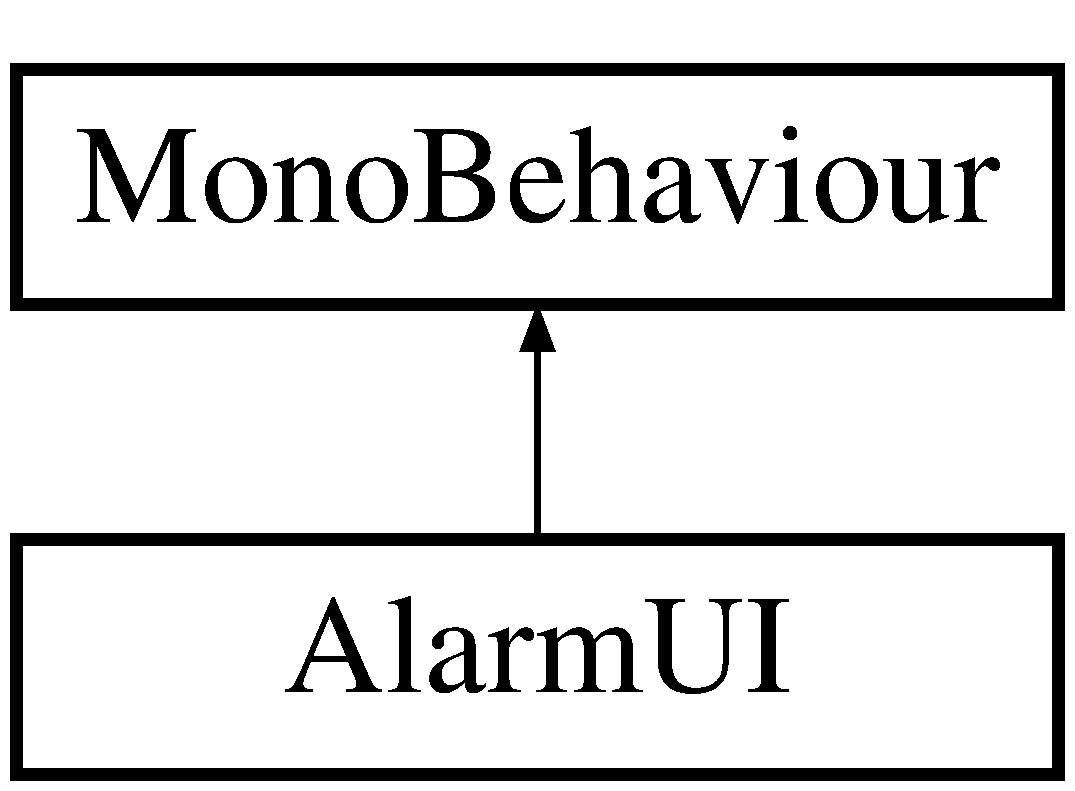
\includegraphics[height=2.000000cm]{class_alarm_u_i}
\end{center}
\end{figure}
\subsection*{Public Member Functions}
\begin{DoxyCompactItemize}
\item 
\mbox{\Hypertarget{class_alarm_u_i_a9b62163cb8e9fc84c398d76cdee02ee1}\label{class_alarm_u_i_a9b62163cb8e9fc84c398d76cdee02ee1}} 
void {\bfseries set\+\_\+alpha} (float alpha)
\item 
\mbox{\Hypertarget{class_alarm_u_i_a9e02cfe3742873a76c89286496e7c6c5}\label{class_alarm_u_i_a9e02cfe3742873a76c89286496e7c6c5}} 
void {\bfseries set\+\_\+color} (Color c)
\item 
\mbox{\Hypertarget{class_alarm_u_i_af591e66d57e7a68dce7233c6a1eb0ad8}\label{class_alarm_u_i_af591e66d57e7a68dce7233c6a1eb0ad8}} 
void {\bfseries fade\+\_\+color} (Color end\+\_\+color, float duration)
\item 
\mbox{\Hypertarget{class_alarm_u_i_a14e4f2abb8b64b3a697a4f23777f6de7}\label{class_alarm_u_i_a14e4f2abb8b64b3a697a4f23777f6de7}} 
void {\bfseries alarm} ()
\end{DoxyCompactItemize}
\subsection*{Public Attributes}
\begin{DoxyCompactItemize}
\item 
\mbox{\Hypertarget{class_alarm_u_i_ab0fdc728cde26889644a5d049572e9ed}\label{class_alarm_u_i_ab0fdc728cde26889644a5d049572e9ed}} 
int {\bfseries size} = 100
\item 
\mbox{\Hypertarget{class_alarm_u_i_af86bb24014cabdd299cb272ced8d7288}\label{class_alarm_u_i_af86bb24014cabdd299cb272ced8d7288}} 
float {\bfseries fade\+\_\+duration} = 1
\item 
\mbox{\Hypertarget{class_alarm_u_i_a78bd9fd39824dec673655d5abde9ab23}\label{class_alarm_u_i_a78bd9fd39824dec673655d5abde9ab23}} 
Image {\bfseries left}
\item 
\mbox{\Hypertarget{class_alarm_u_i_a82a2c9cccd6006726f290c7170c34f86}\label{class_alarm_u_i_a82a2c9cccd6006726f290c7170c34f86}} 
Image {\bfseries bot}
\item 
\mbox{\Hypertarget{class_alarm_u_i_aaec62da22f7efc761dfb29ba20c61c32}\label{class_alarm_u_i_aaec62da22f7efc761dfb29ba20c61c32}} 
Image {\bfseries right}
\item 
\mbox{\Hypertarget{class_alarm_u_i_a0b6deced69b4466f8fb03cf4d945b4b0}\label{class_alarm_u_i_a0b6deced69b4466f8fb03cf4d945b4b0}} 
Image {\bfseries top}
\item 
\mbox{\Hypertarget{class_alarm_u_i_aafaba46ad3e7cc0bea53caf79039326b}\label{class_alarm_u_i_aafaba46ad3e7cc0bea53caf79039326b}} 
List$<$ Image $>$ {\bfseries all\+Images}
\end{DoxyCompactItemize}
\subsection*{Static Public Attributes}
\begin{DoxyCompactItemize}
\item 
\mbox{\Hypertarget{class_alarm_u_i_a5887790cd7ad779fd85a748edd1a5750}\label{class_alarm_u_i_a5887790cd7ad779fd85a748edd1a5750}} 
static \hyperlink{class_alarm_u_i}{Alarm\+UI} {\bfseries alarm\+UI}
\end{DoxyCompactItemize}


The documentation for this class was generated from the following file\+:\begin{DoxyCompactItemize}
\item 
/\+Users/\+Leonard/\+Desktop/\+Stor\+Trok/\+Stor Trok/\+Assets/\+Stor Trok/\+Scripts/\+U\+I/Alarm\+U\+I.\+cs\end{DoxyCompactItemize}

\hypertarget{class_angle_range}{}\section{Angle\+Range Class Reference}
\label{class_angle_range}\index{Angle\+Range@{Angle\+Range}}
\subsection*{Public Member Functions}
\begin{DoxyCompactItemize}
\item 
\mbox{\Hypertarget{class_angle_range_a15fbd365c40c3e4d94e084a0b326388d}\label{class_angle_range_a15fbd365c40c3e4d94e084a0b326388d}} 
{\bfseries Angle\+Range} (float min, float max)
\item 
\mbox{\Hypertarget{class_angle_range_ab52bad939f59a22c7a2a5c3d5ec345fb}\label{class_angle_range_ab52bad939f59a22c7a2a5c3d5ec345fb}} 
bool {\bfseries contains\+\_\+number} (float number)
\end{DoxyCompactItemize}
\subsection*{Public Attributes}
\begin{DoxyCompactItemize}
\item 
\mbox{\Hypertarget{class_angle_range_a70ae79b50baedb3091d9b6829f4e924d}\label{class_angle_range_a70ae79b50baedb3091d9b6829f4e924d}} 
float {\bfseries min}
\item 
\mbox{\Hypertarget{class_angle_range_a20b198dd16cd264992dcea5cb6a82fff}\label{class_angle_range_a20b198dd16cd264992dcea5cb6a82fff}} 
float {\bfseries max}
\end{DoxyCompactItemize}


The documentation for this class was generated from the following file\+:\begin{DoxyCompactItemize}
\item 
/\+Users/\+Leonard/\+Desktop/\+Stor\+Trok/\+Stor Trok/\+Assets/\+Stor Trok/\+Scripts/Utils.\+cs\end{DoxyCompactItemize}

\hypertarget{class_asteroid}{}\section{Asteroid Class Reference}
\label{class_asteroid}\index{Asteroid@{Asteroid}}
Inheritance diagram for Asteroid\+:\begin{figure}[H]
\begin{center}
\leavevmode
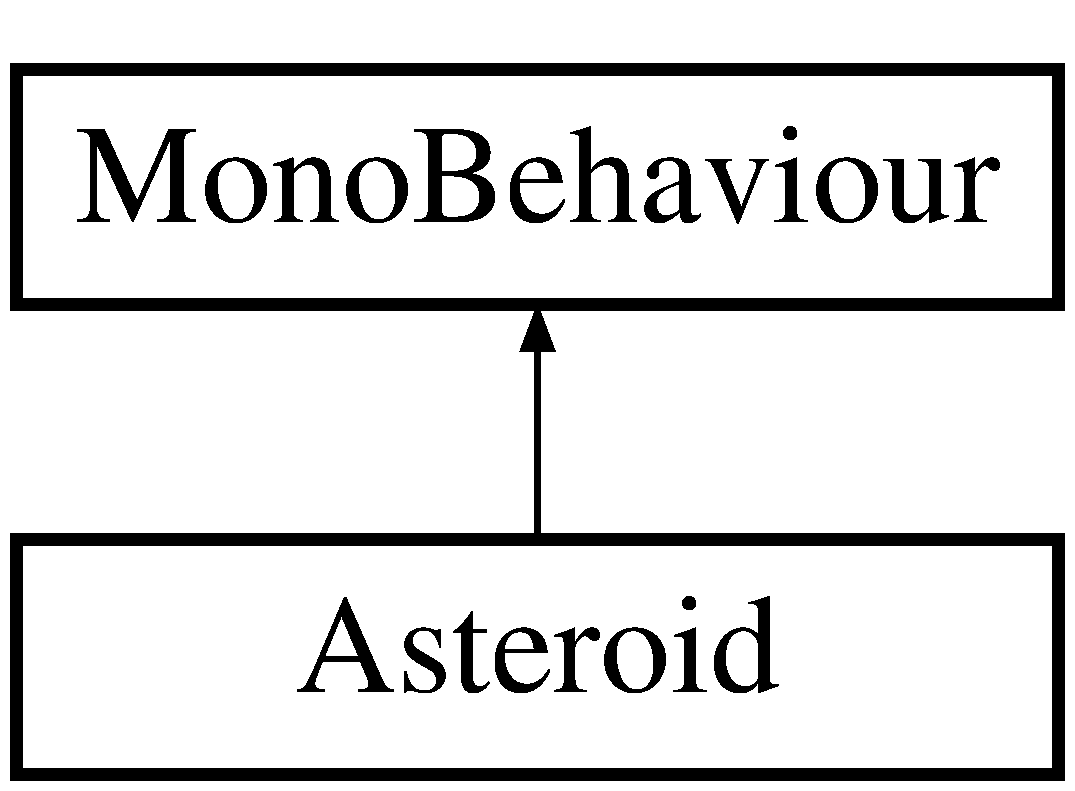
\includegraphics[height=2.000000cm]{class_asteroid}
\end{center}
\end{figure}
\subsection*{Public Attributes}
\begin{DoxyCompactItemize}
\item 
\mbox{\Hypertarget{class_asteroid_a10ff7dab44740dd98ed44ec9f6386021}\label{class_asteroid_a10ff7dab44740dd98ed44ec9f6386021}} 
Game\+Object {\bfseries target\+\_\+object}
\item 
\mbox{\Hypertarget{class_asteroid_a72a8b00fa29cafb864297764b594fa08}\label{class_asteroid_a72a8b00fa29cafb864297764b594fa08}} 
float {\bfseries damage}
\item 
\mbox{\Hypertarget{class_asteroid_a2113dbc14a1bb6298100b979de52f68d}\label{class_asteroid_a2113dbc14a1bb6298100b979de52f68d}} 
float {\bfseries shield\+\_\+pen}
\item 
\mbox{\Hypertarget{class_asteroid_aa57424523dd19579e82ae7aed657be95}\label{class_asteroid_aa57424523dd19579e82ae7aed657be95}} 
float {\bfseries acceleration} = 100
\end{DoxyCompactItemize}


The documentation for this class was generated from the following file\+:\begin{DoxyCompactItemize}
\item 
/\+Users/\+Leonard/\+Desktop/\+Stor\+Trok/\+Stor Trok/\+Assets/\+Stor Trok/\+Scripts/Asteroid.\+cs\end{DoxyCompactItemize}

\hypertarget{class_audio_assets}{}\section{Audio\+Assets Class Reference}
\label{class_audio_assets}\index{Audio\+Assets@{Audio\+Assets}}
Inheritance diagram for Audio\+Assets\+:\begin{figure}[H]
\begin{center}
\leavevmode
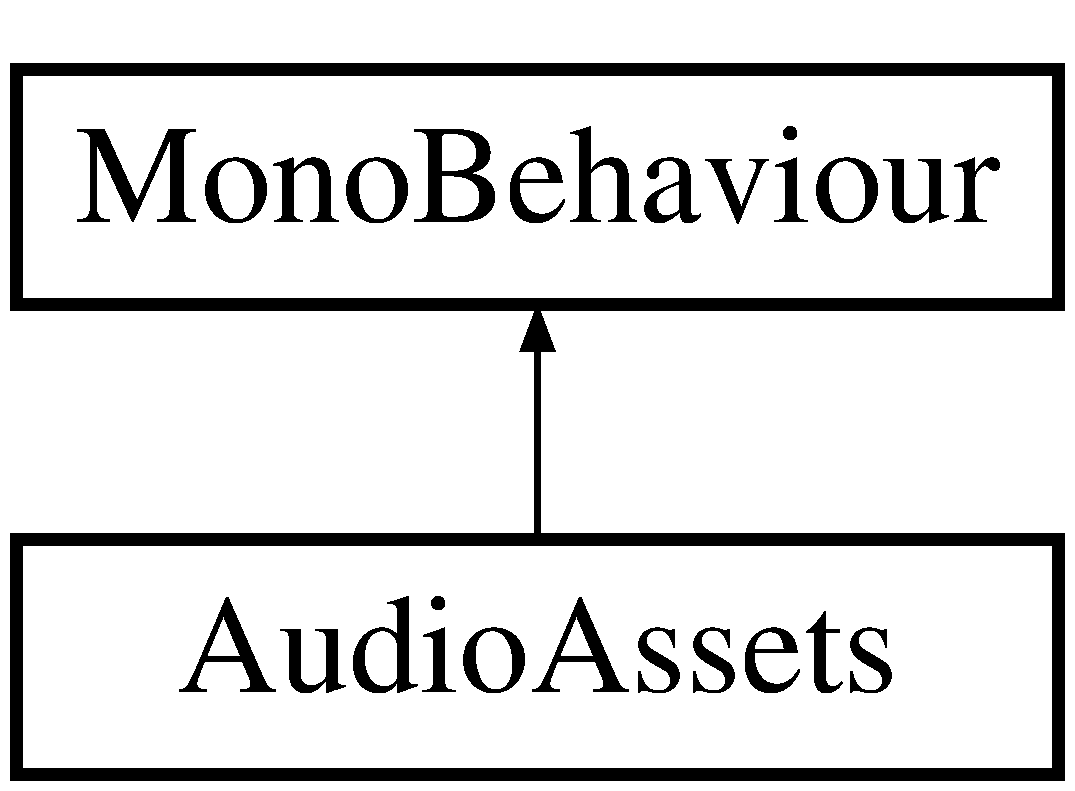
\includegraphics[height=2.000000cm]{class_audio_assets}
\end{center}
\end{figure}
\subsection*{Public Attributes}
\begin{DoxyCompactItemize}
\item 
\mbox{\Hypertarget{class_audio_assets_a6c0372672280f3c1a7e289c699d01bd6}\label{class_audio_assets_a6c0372672280f3c1a7e289c699d01bd6}} 
Audio\+Clip \mbox{[}$\,$\mbox{]} {\bfseries explosions}
\item 
\mbox{\Hypertarget{class_audio_assets_a2c6105d12139e154693c8776fdec5f00}\label{class_audio_assets_a2c6105d12139e154693c8776fdec5f00}} 
Audio\+Clip \mbox{[}$\,$\mbox{]} {\bfseries phasers}
\end{DoxyCompactItemize}
\subsection*{Static Public Attributes}
\begin{DoxyCompactItemize}
\item 
\mbox{\Hypertarget{class_audio_assets_a32df5d1b5c2799c970b00f4bac8cd9dc}\label{class_audio_assets_a32df5d1b5c2799c970b00f4bac8cd9dc}} 
static \hyperlink{class_audio_assets}{Audio\+Assets} {\bfseries audio\+\_\+assets}
\end{DoxyCompactItemize}


The documentation for this class was generated from the following file\+:\begin{DoxyCompactItemize}
\item 
/\+Users/\+Leonard/\+Desktop/\+Stor\+Trok/\+Stor Trok/\+Assets/\+Stor Trok/\+Scripts/\+Asset\+Classes/Audio\+Assets.\+cs\end{DoxyCompactItemize}

\hypertarget{class_auspuff}{}\section{Auspuff Class Reference}
\label{class_auspuff}\index{Auspuff@{Auspuff}}
Inheritance diagram for Auspuff\+:\begin{figure}[H]
\begin{center}
\leavevmode
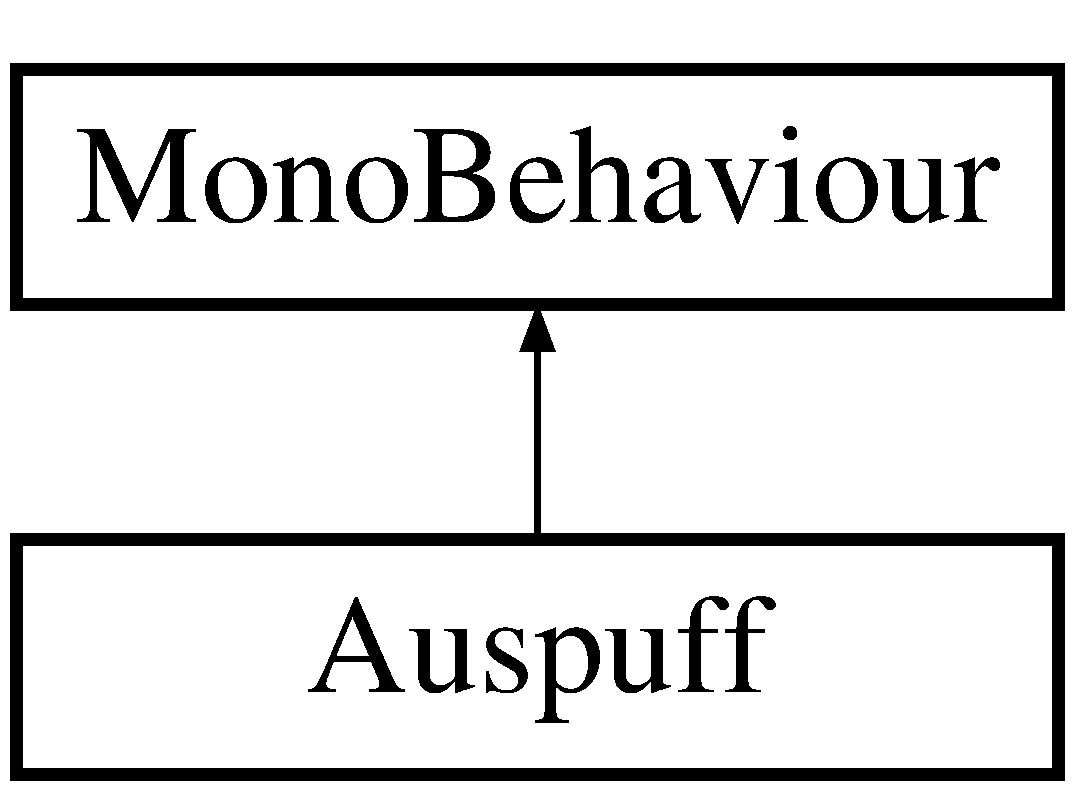
\includegraphics[height=2.000000cm]{class_auspuff}
\end{center}
\end{figure}
\subsection*{Public Attributes}
\begin{DoxyCompactItemize}
\item 
\mbox{\Hypertarget{class_auspuff_a638bf5bf159a0aae732a9873180a7a6c}\label{class_auspuff_a638bf5bf159a0aae732a9873180a7a6c}} 
Line\+Renderer {\bfseries line\+\_\+renderer}
\item 
\mbox{\Hypertarget{class_auspuff_a304d521eeb66988f3a41094b498368ab}\label{class_auspuff_a304d521eeb66988f3a41094b498368ab}} 
int {\bfseries number\+\_\+of\+\_\+positions} = 60
\item 
\mbox{\Hypertarget{class_auspuff_a46a8ef5df8bcf1d97849bb0c0c647923}\label{class_auspuff_a46a8ef5df8bcf1d97849bb0c0c647923}} 
const bool {\bfseries use\+\_\+unity\+\_\+trailrenderer} = true
\end{DoxyCompactItemize}


The documentation for this class was generated from the following file\+:\begin{DoxyCompactItemize}
\item 
/\+Users/\+Leonard/\+Desktop/\+Stor\+Trok/\+Stor Trok/\+Assets/\+Stor Trok/\+Scripts/\+Player/Auspuff.\+cs\end{DoxyCompactItemize}

\hypertarget{class_bezier_curve}{}\section{Bezier\+Curve Class Reference}
\label{class_bezier_curve}\index{Bezier\+Curve@{Bezier\+Curve}}
Inheritance diagram for Bezier\+Curve\+:\begin{figure}[H]
\begin{center}
\leavevmode
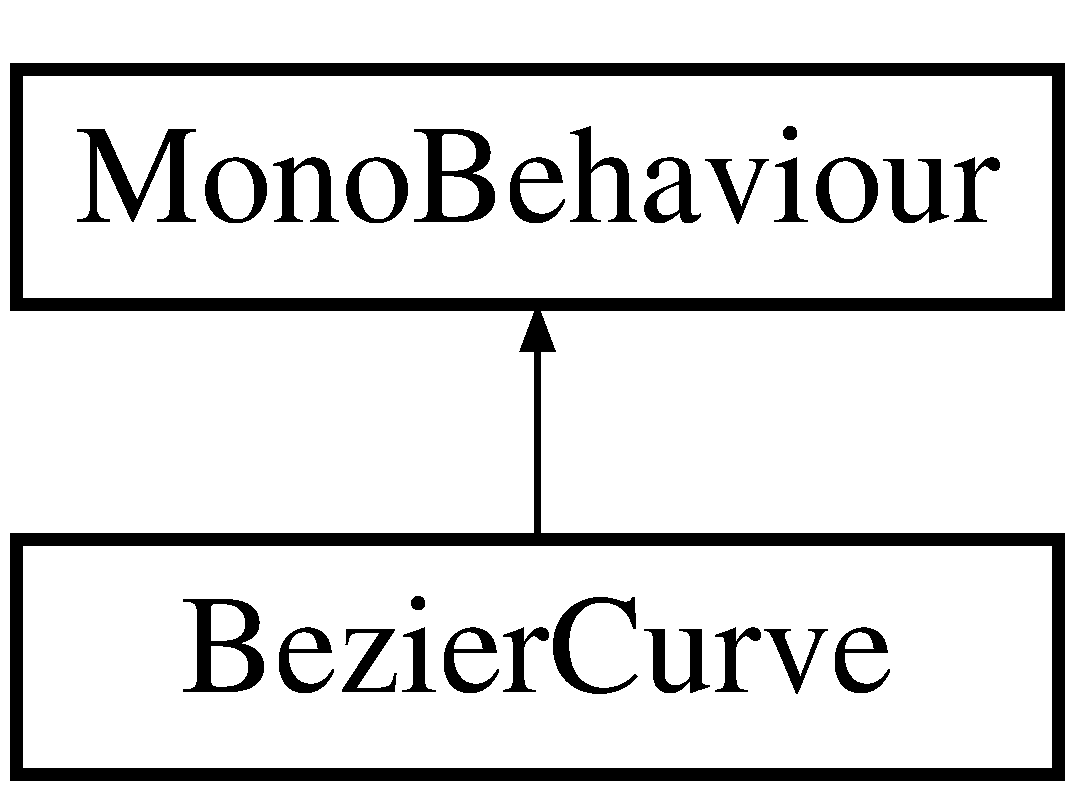
\includegraphics[height=2.000000cm]{class_bezier_curve}
\end{center}
\end{figure}
\subsection*{Public Attributes}
\begin{DoxyCompactItemize}
\item 
\mbox{\Hypertarget{class_bezier_curve_acbd74aa32496cfc588d30c3200662ba8}\label{class_bezier_curve_acbd74aa32496cfc588d30c3200662ba8}} 
int {\bfseries number\+\_\+of\+\_\+points\+\_\+on\+\_\+curve} = 100
\item 
\mbox{\Hypertarget{class_bezier_curve_aca442eafb5988a261b23276c36fc279f}\label{class_bezier_curve_aca442eafb5988a261b23276c36fc279f}} 
Transform \mbox{[}$\,$\mbox{]} {\bfseries controll\+\_\+points} = new Transform\mbox{[}0\mbox{]}
\end{DoxyCompactItemize}


The documentation for this class was generated from the following file\+:\begin{DoxyCompactItemize}
\item 
/\+Users/\+Leonard/\+Desktop/\+Stor\+Trok/\+Stor Trok/\+Assets/\+Stor Trok/\+Scripts/\+Tests/Bezier\+Curve.\+cs\end{DoxyCompactItemize}

\hypertarget{class_borg_cube}{}\section{Borg\+Cube Class Reference}
\label{class_borg_cube}\index{Borg\+Cube@{Borg\+Cube}}
Inheritance diagram for Borg\+Cube\+:\begin{figure}[H]
\begin{center}
\leavevmode
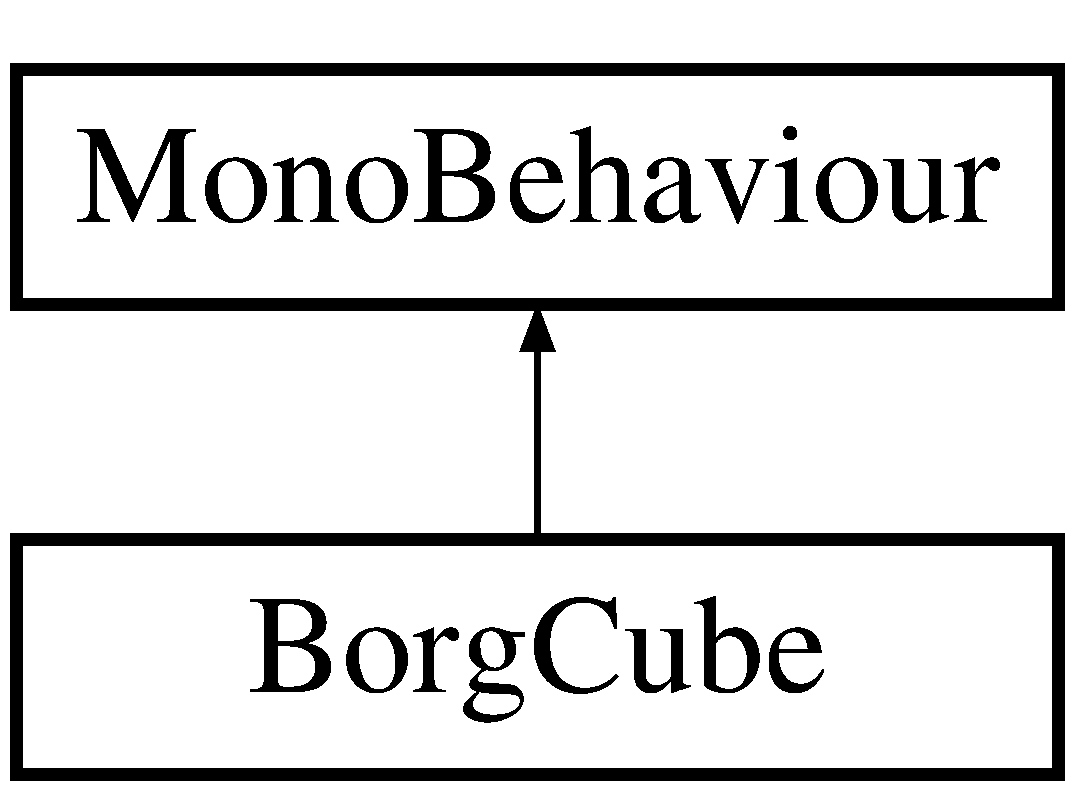
\includegraphics[height=2.000000cm]{class_borg_cube}
\end{center}
\end{figure}
\subsection*{Public Attributes}
\begin{DoxyCompactItemize}
\item 
\mbox{\Hypertarget{class_borg_cube_ab24a0396db035b845d9a2ed2c22fd62d}\label{class_borg_cube_ab24a0396db035b845d9a2ed2c22fd62d}} 
\hyperlink{class_computer_player}{Computer\+Player} {\bfseries computer\+\_\+player}
\end{DoxyCompactItemize}


The documentation for this class was generated from the following file\+:\begin{DoxyCompactItemize}
\item 
/\+Users/\+Leonard/\+Desktop/\+Stor\+Trok/\+Stor Trok/\+Assets/\+Stor Trok/\+Scripts/\+Computer\+Players/\+Spaceships/Borg\+Cube.\+cs\end{DoxyCompactItemize}

\hypertarget{class_camera_script}{}\section{Camera\+Script Class Reference}
\label{class_camera_script}\index{Camera\+Script@{Camera\+Script}}
Inheritance diagram for Camera\+Script\+:\begin{figure}[H]
\begin{center}
\leavevmode
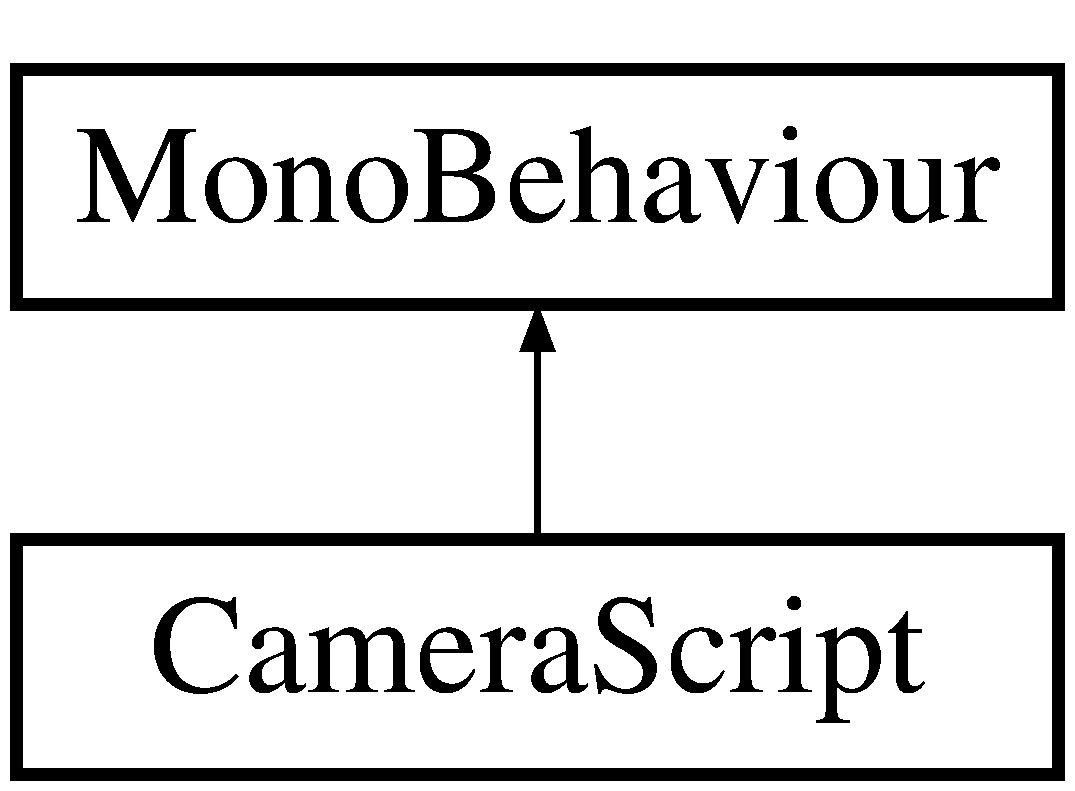
\includegraphics[height=2.000000cm]{class_camera_script}
\end{center}
\end{figure}
\subsection*{Public Member Functions}
\begin{DoxyCompactItemize}
\item 
\mbox{\Hypertarget{class_camera_script_acb2cca3e4fcf99850d937cf05f167014}\label{class_camera_script_acb2cca3e4fcf99850d937cf05f167014}} 
void {\bfseries lookat\+\_\+point} (Vector3 point)
\end{DoxyCompactItemize}
\subsection*{Public Attributes}
\begin{DoxyCompactItemize}
\item 
\mbox{\Hypertarget{class_camera_script_a6e44b5bc41c6ae01f37bbaebcf5970c2}\label{class_camera_script_a6e44b5bc41c6ae01f37bbaebcf5970c2}} 
float {\bfseries camera\+\_\+ortho\+\_\+size} = 30
\item 
\mbox{\Hypertarget{class_camera_script_ab045581c45e499bdbf45a4b851ccc348}\label{class_camera_script_ab045581c45e499bdbf45a4b851ccc348}} 
float {\bfseries camera\+\_\+angle} = 30
\item 
\mbox{\Hypertarget{class_camera_script_a1217a340c62b4bae90b9e6ce025639bb}\label{class_camera_script_a1217a340c62b4bae90b9e6ce025639bb}} 
float {\bfseries mouse\+\_\+x\+\_\+sensitivity} = 2
\item 
\mbox{\Hypertarget{class_camera_script_a05b4e9ac080a524baf6acd9069c1690c}\label{class_camera_script_a05b4e9ac080a524baf6acd9069c1690c}} 
float {\bfseries mouse\+\_\+y\+\_\+sensitivity} = 2
\item 
\mbox{\Hypertarget{class_camera_script_a0d20cdfac93124cc8779f2c618d87118}\label{class_camera_script_a0d20cdfac93124cc8779f2c618d87118}} 
Game\+Object {\bfseries camera\+\_\+center}
\item 
\mbox{\Hypertarget{class_camera_script_a91f4127c39260706fdc3db3ad60c0eeb}\label{class_camera_script_a91f4127c39260706fdc3db3ad60c0eeb}} 
bool {\bfseries lookat\+\_\+player\+\_\+and\+\_\+controllable} = true
\item 
\mbox{\Hypertarget{class_camera_script_a12cea733980757a4cd48d91717daf607}\label{class_camera_script_a12cea733980757a4cd48d91717daf607}} 
Game\+Object {\bfseries lookat\+\_\+object}
\end{DoxyCompactItemize}
\subsection*{Static Public Attributes}
\begin{DoxyCompactItemize}
\item 
\mbox{\Hypertarget{class_camera_script_adfea0fdca00f979407b479a33230a259}\label{class_camera_script_adfea0fdca00f979407b479a33230a259}} 
static \hyperlink{class_camera_script}{Camera\+Script} {\bfseries camera\+\_\+script}
\end{DoxyCompactItemize}


The documentation for this class was generated from the following file\+:\begin{DoxyCompactItemize}
\item 
/\+Users/\+Leonard/\+Desktop/\+Stor\+Trok/\+Stor Trok/\+Assets/\+Stor Trok/\+Scripts/\+Player/Camera\+Script.\+cs\end{DoxyCompactItemize}

\hypertarget{class_camera_viewporttest}{}\section{Camera\+Viewporttest Class Reference}
\label{class_camera_viewporttest}\index{Camera\+Viewporttest@{Camera\+Viewporttest}}
Inheritance diagram for Camera\+Viewporttest\+:\begin{figure}[H]
\begin{center}
\leavevmode
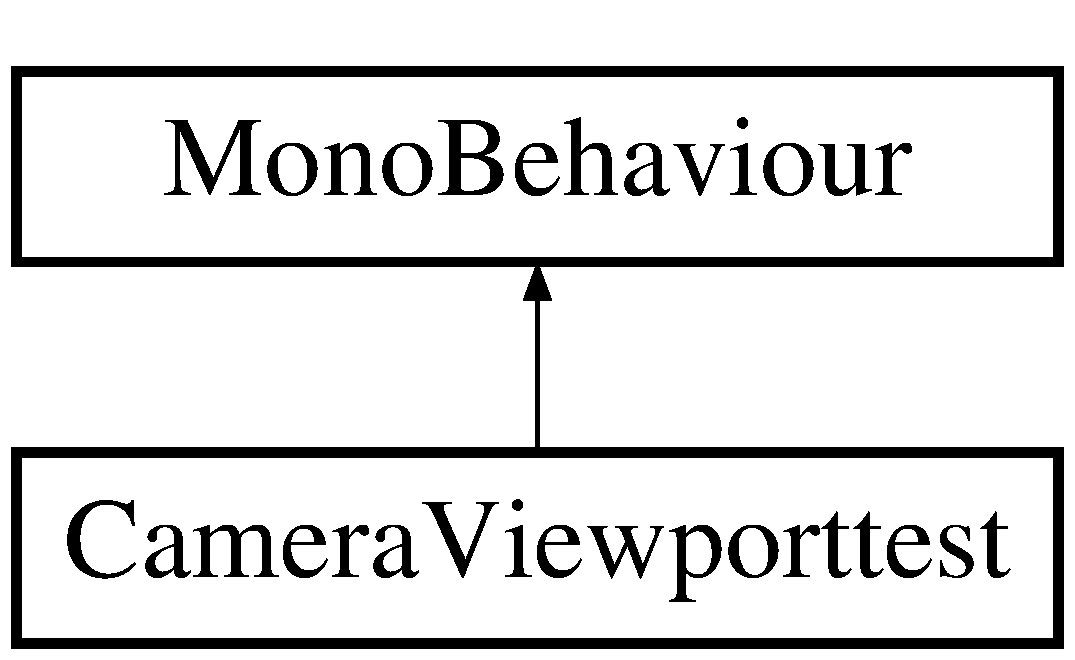
\includegraphics[height=2.000000cm]{class_camera_viewporttest}
\end{center}
\end{figure}


The documentation for this class was generated from the following file\+:\begin{DoxyCompactItemize}
\item 
/\+Users/\+Leonard/\+Desktop/\+Stor\+Trok/\+Stor Trok/\+Assets/\+Stor Trok/\+Scripts/\+Tests/Camera\+Viewporttest.\+cs\end{DoxyCompactItemize}

\hypertarget{class_character_controller_v2}{}\section{Character\+Controller\+V2 Class Reference}
\label{class_character_controller_v2}\index{Character\+Controller\+V2@{Character\+Controller\+V2}}
Inheritance diagram for Character\+Controller\+V2\+:\begin{figure}[H]
\begin{center}
\leavevmode
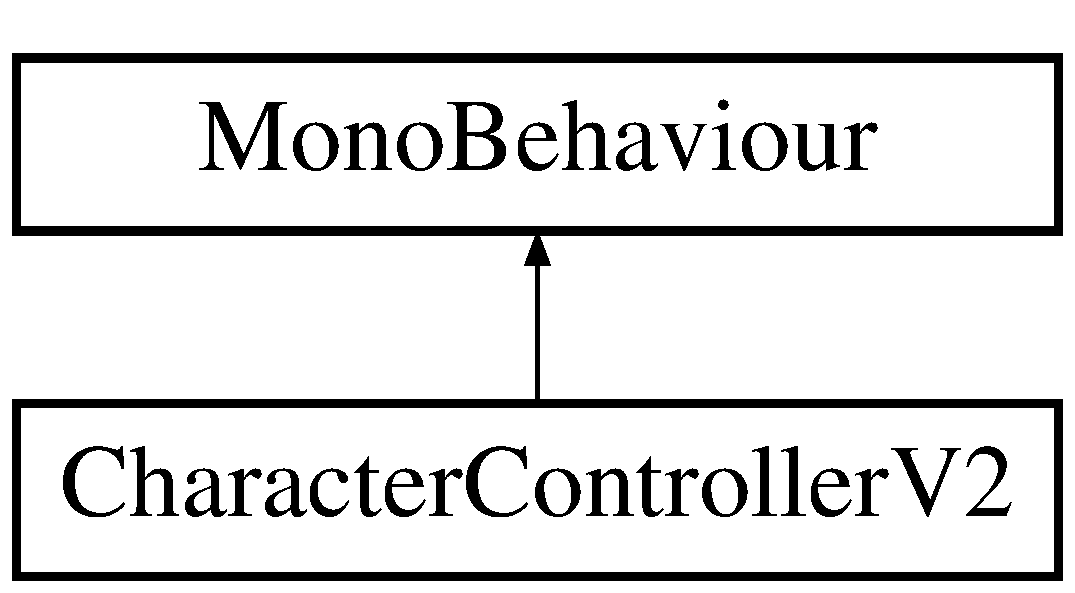
\includegraphics[height=2.000000cm]{class_character_controller_v2}
\end{center}
\end{figure}


The documentation for this class was generated from the following file\+:\begin{DoxyCompactItemize}
\item 
/\+Users/\+Leonard/\+Desktop/\+Stor\+Trok/\+Stor Trok/\+Assets/\+Stor Trok/\+Scripts/\+Shop/Character\+Controller\+V2.\+cs\end{DoxyCompactItemize}

\hypertarget{class_cloaking_device}{}\section{Cloaking\+Device Class Reference}
\label{class_cloaking_device}\index{Cloaking\+Device@{Cloaking\+Device}}
Inheritance diagram for Cloaking\+Device\+:\begin{figure}[H]
\begin{center}
\leavevmode
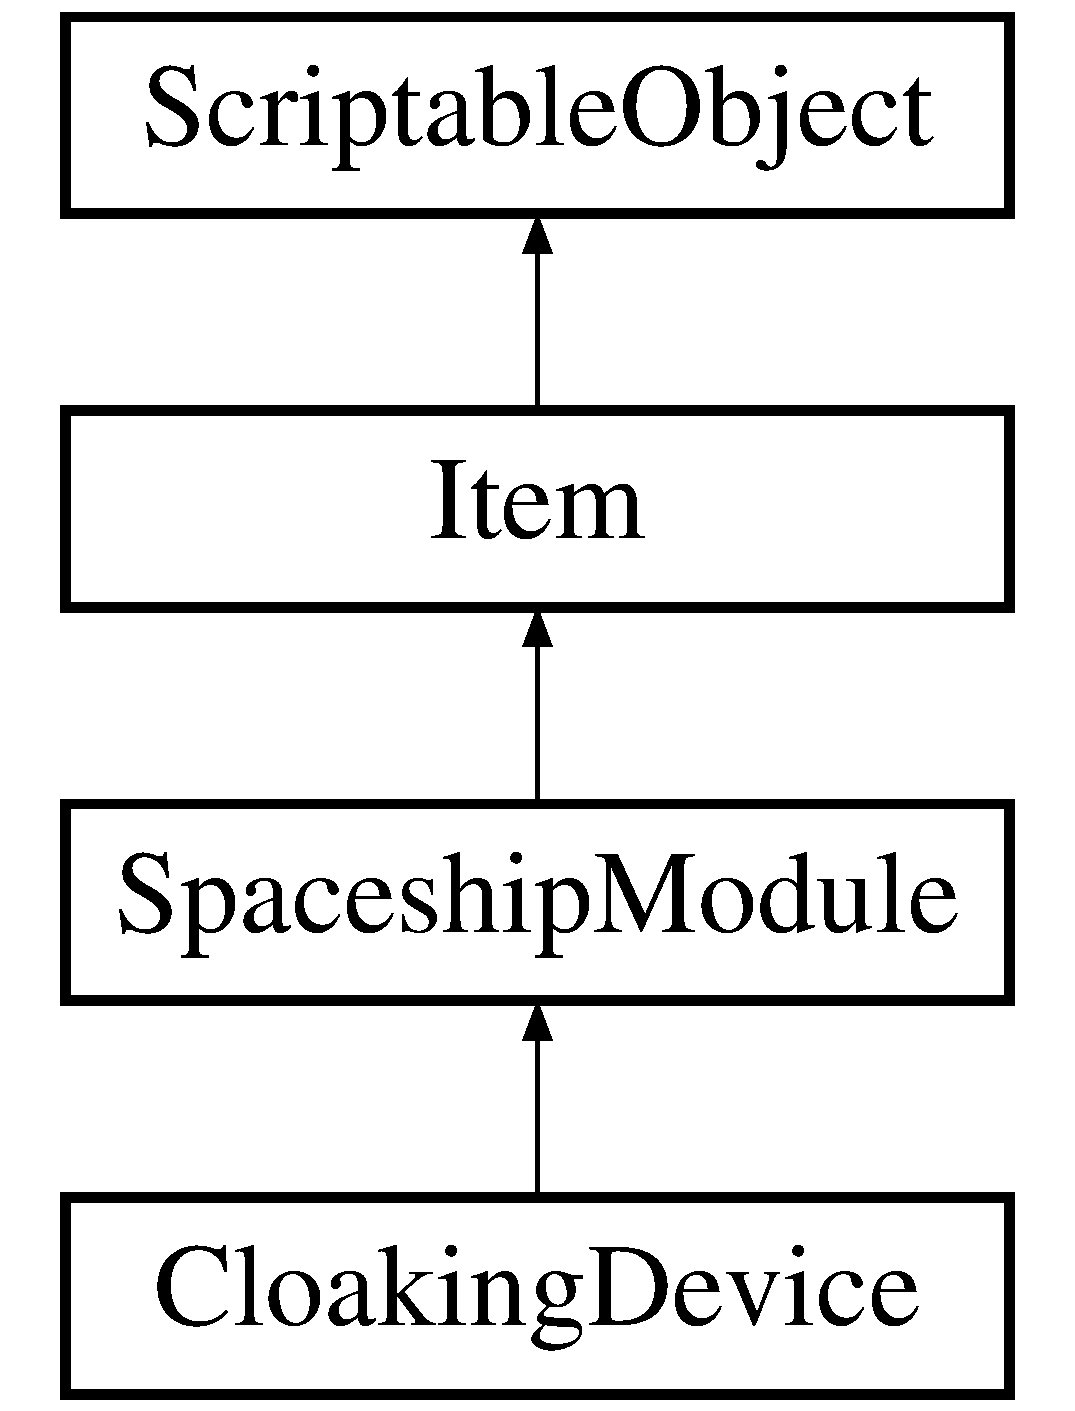
\includegraphics[height=4.000000cm]{class_cloaking_device}
\end{center}
\end{figure}
\subsection*{Public Member Functions}
\begin{DoxyCompactItemize}
\item 
\mbox{\Hypertarget{class_cloaking_device_a37211f77adc401c5abf08a5e5fcd9f05}\label{class_cloaking_device_a37211f77adc401c5abf08a5e5fcd9f05}} 
override void {\bfseries animation} ()
\end{DoxyCompactItemize}
\subsection*{Public Attributes}
\begin{DoxyCompactItemize}
\item 
\mbox{\Hypertarget{class_cloaking_device_acc053a4955de25da2705a3362f568965}\label{class_cloaking_device_acc053a4955de25da2705a3362f568965}} 
float {\bfseries speed\+\_\+buff} = 1.\+3f
\item 
\mbox{\Hypertarget{class_cloaking_device_ace548b4010af49cc83b18f859e501b8c}\label{class_cloaking_device_ace548b4010af49cc83b18f859e501b8c}} 
float {\bfseries damage\+\_\+buff} = 10f
\end{DoxyCompactItemize}
\subsection*{Additional Inherited Members}


The documentation for this class was generated from the following file\+:\begin{DoxyCompactItemize}
\item 
/\+Users/\+Leonard/\+Desktop/\+Stor\+Trok/\+Stor Trok/\+Assets/\+Stor Trok/\+Scripts/\+Items/\+Spaceship\+Modules/Cloaking\+Device.\+cs\end{DoxyCompactItemize}

\hypertarget{class_computer_movement_with_player_data}{}\section{Computer\+Movement\+With\+Player\+Data Class Reference}
\label{class_computer_movement_with_player_data}\index{Computer\+Movement\+With\+Player\+Data@{Computer\+Movement\+With\+Player\+Data}}
Inheritance diagram for Computer\+Movement\+With\+Player\+Data\+:\begin{figure}[H]
\begin{center}
\leavevmode
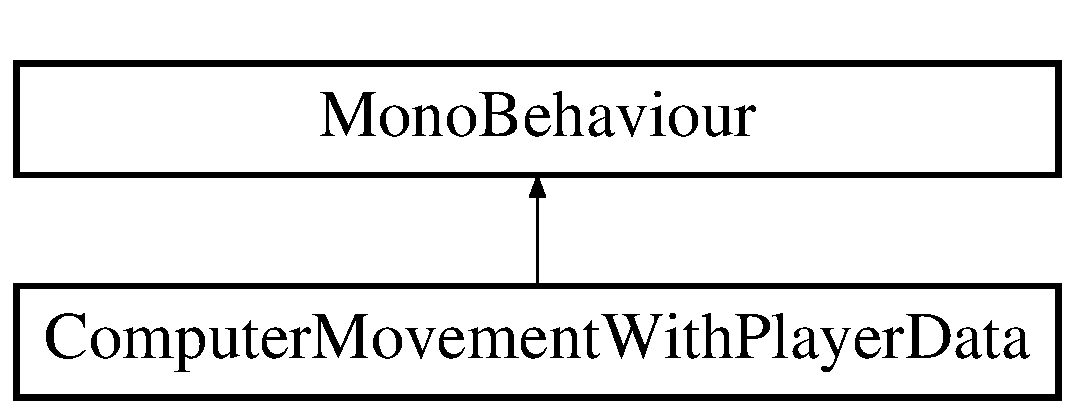
\includegraphics[height=2.000000cm]{class_computer_movement_with_player_data}
\end{center}
\end{figure}
\subsection*{Public Attributes}
\begin{DoxyCompactItemize}
\item 
\mbox{\Hypertarget{class_computer_movement_with_player_data_ae59e2f2887983cfce860f28a383938b2}\label{class_computer_movement_with_player_data_ae59e2f2887983cfce860f28a383938b2}} 
float {\bfseries return\+\_\+to\+\_\+enemy\+\_\+distance} = 1000
\item 
\mbox{\Hypertarget{class_computer_movement_with_player_data_a367804093dad6261c476c943b1115de7}\label{class_computer_movement_with_player_data_a367804093dad6261c476c943b1115de7}} 
float {\bfseries return\+\_\+to\+\_\+enemy\+\_\+target\+\_\+distance} = 500
\end{DoxyCompactItemize}


The documentation for this class was generated from the following file\+:\begin{DoxyCompactItemize}
\item 
/\+Users/\+Leonard/\+Desktop/\+Stor\+Trok/\+Stor Trok/\+Assets/\+Stor Trok/\+Scripts/\+Computer\+Players/\+Movement\+Types/\+Movement\+With\+Player\+Data/Computer\+Movement\+With\+Player\+Data.\+cs\end{DoxyCompactItemize}

\hypertarget{class_computer_player}{}\section{Computer\+Player Class Reference}
\label{class_computer_player}\index{Computer\+Player@{Computer\+Player}}
Inheritance diagram for Computer\+Player\+:\begin{figure}[H]
\begin{center}
\leavevmode
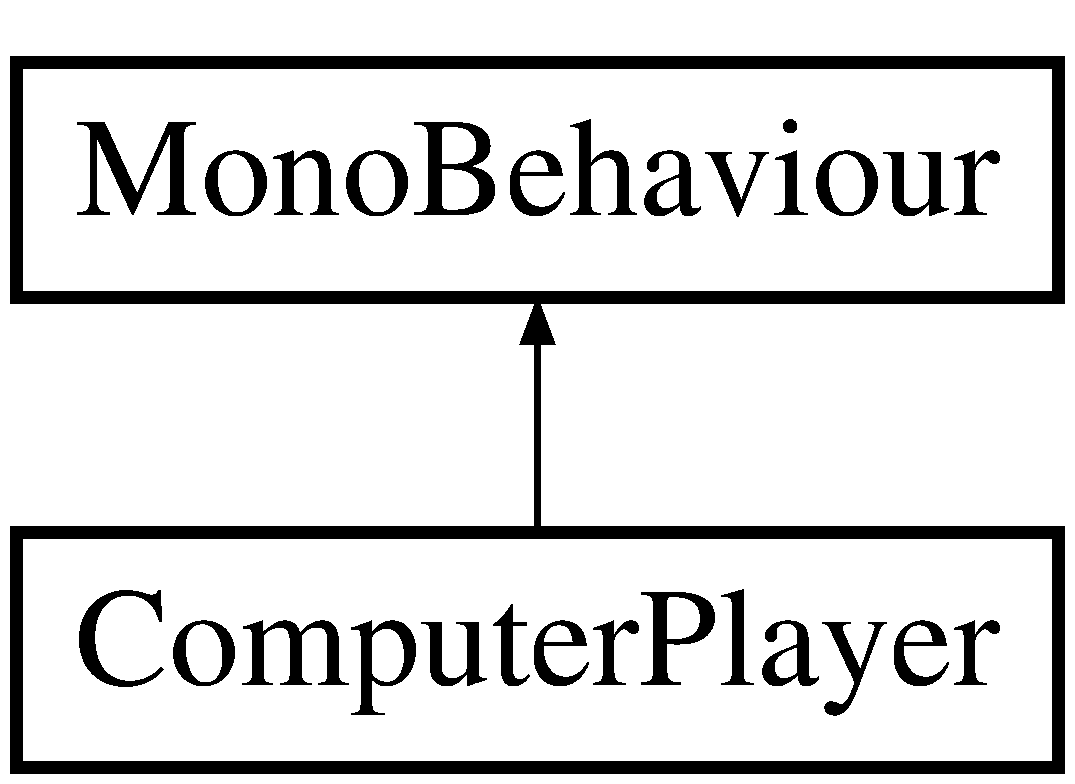
\includegraphics[height=2.000000cm]{class_computer_player}
\end{center}
\end{figure}
\subsection*{Public Member Functions}
\begin{DoxyCompactItemize}
\item 
\mbox{\Hypertarget{class_computer_player_a0b5dc7186a115e08f15a45525dfdf48e}\label{class_computer_player_a0b5dc7186a115e08f15a45525dfdf48e}} 
List$<$ \hyperlink{class_spaceship}{Spaceship} $>$ {\bfseries get\+\_\+enemies} ()
\item 
\mbox{\Hypertarget{class_computer_player_a2a25d6a48ffe69c4f68b2142251f6561}\label{class_computer_player_a2a25d6a48ffe69c4f68b2142251f6561}} 
int {\bfseries get\+\_\+enemy\+\_\+layer} ()
\item 
\mbox{\Hypertarget{class_computer_player_a87ca5cde4b9d5796b4e1442dd0d49573}\label{class_computer_player_a87ca5cde4b9d5796b4e1442dd0d49573}} 
void {\bfseries enable\+\_\+movement} ()
\item 
\mbox{\Hypertarget{class_computer_player_a62a1be22712b133ef57e8b01b54f0595}\label{class_computer_player_a62a1be22712b133ef57e8b01b54f0595}} 
void {\bfseries disable\+\_\+movement} ()
\end{DoxyCompactItemize}
\subsection*{Public Attributes}
\begin{DoxyCompactItemize}
\item 
\mbox{\Hypertarget{class_computer_player_a1a14ec11162eef9cfc4542ea8506cbe2}\label{class_computer_player_a1a14ec11162eef9cfc4542ea8506cbe2}} 
Game\+Object {\bfseries selected\+\_\+enemy}
\item 
\mbox{\Hypertarget{class_computer_player_a6d0f8ad95561dd15d67f90a2abe732cd}\label{class_computer_player_a6d0f8ad95561dd15d67f90a2abe732cd}} 
Mono\+Behaviour {\bfseries movement\+\_\+script}
\item 
\mbox{\Hypertarget{class_computer_player_aaf21dbd67f917b8febbf4d88c6765a29}\label{class_computer_player_aaf21dbd67f917b8febbf4d88c6765a29}} 
bool {\bfseries no\+\_\+movement} = false
\end{DoxyCompactItemize}
\subsection*{Properties}
\begin{DoxyCompactItemize}
\item 
\mbox{\Hypertarget{class_computer_player_a7e4609385eec3f637f8e7bbcd328a9a3}\label{class_computer_player_a7e4609385eec3f637f8e7bbcd328a9a3}} 
\hyperlink{class_spaceship}{Spaceship} {\bfseries spaceship}\hspace{0.3cm}{\ttfamily  \mbox{[}get\mbox{]}}
\end{DoxyCompactItemize}


The documentation for this class was generated from the following file\+:\begin{DoxyCompactItemize}
\item 
/\+Users/\+Leonard/\+Desktop/\+Stor\+Trok/\+Stor Trok/\+Assets/\+Stor Trok/\+Scripts/\+Computer\+Players/Computer\+Player.\+cs\end{DoxyCompactItemize}

\hypertarget{class_death_timer}{}\section{Death\+Timer Class Reference}
\label{class_death_timer}\index{Death\+Timer@{Death\+Timer}}
Inheritance diagram for Death\+Timer\+:\begin{figure}[H]
\begin{center}
\leavevmode
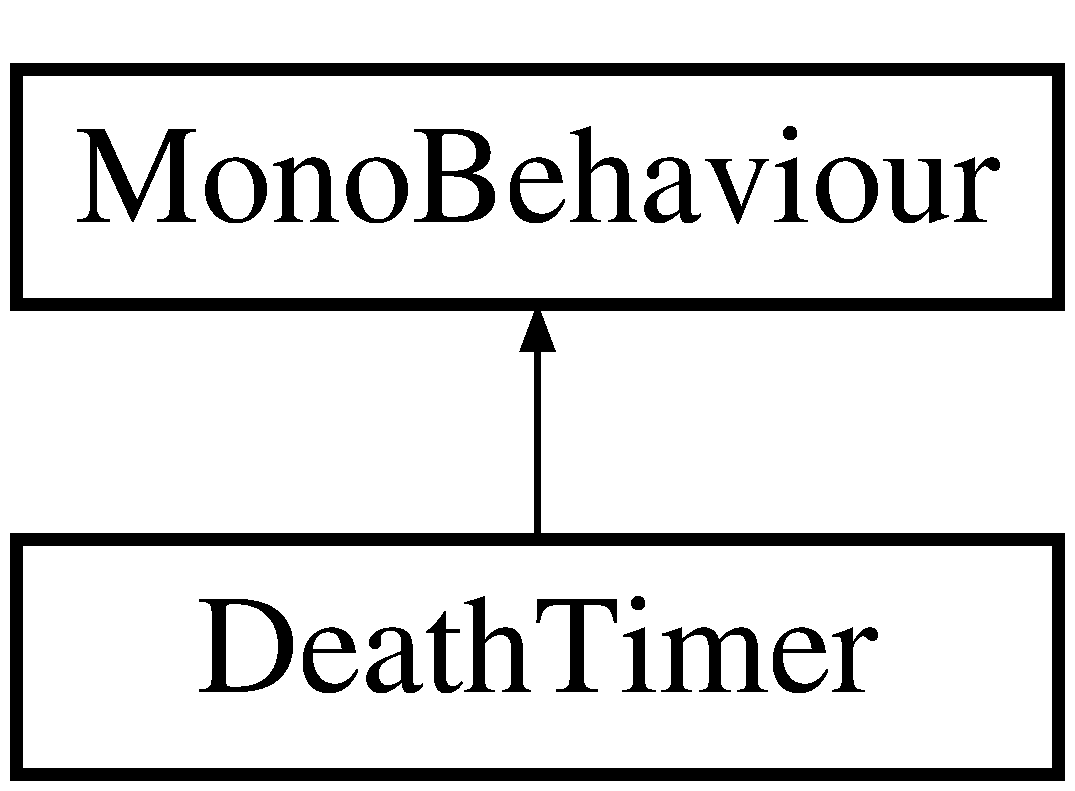
\includegraphics[height=2.000000cm]{class_death_timer}
\end{center}
\end{figure}
\subsection*{Public Member Functions}
\begin{DoxyCompactItemize}
\item 
\mbox{\Hypertarget{class_death_timer_a96dd059f241358fd105e754a065e3416}\label{class_death_timer_a96dd059f241358fd105e754a065e3416}} 
void {\bfseries respawn\+\_\+button\+\_\+clicked} ()
\end{DoxyCompactItemize}
\subsection*{Public Attributes}
\begin{DoxyCompactItemize}
\item 
\mbox{\Hypertarget{class_death_timer_a8d538b8a6e2382912768a7d1436a0421}\label{class_death_timer_a8d538b8a6e2382912768a7d1436a0421}} 
float {\bfseries timer\+\_\+start}
\item 
\mbox{\Hypertarget{class_death_timer_a5b8900b148c5ff0190b718a158516f7f}\label{class_death_timer_a5b8900b148c5ff0190b718a158516f7f}} 
const float {\bfseries death\+\_\+timer} = 10
\item 
\mbox{\Hypertarget{class_death_timer_a9d87e936e7aa4727b020d054cd3dedcb}\label{class_death_timer_a9d87e936e7aa4727b020d054cd3dedcb}} 
Text {\bfseries timer\+\_\+text}
\item 
\mbox{\Hypertarget{class_death_timer_a01d6fc809fe54b19f68d02320c2597ec}\label{class_death_timer_a01d6fc809fe54b19f68d02320c2597ec}} 
Button {\bfseries respawn\+\_\+button}
\end{DoxyCompactItemize}


The documentation for this class was generated from the following file\+:\begin{DoxyCompactItemize}
\item 
/\+Users/\+Leonard/\+Desktop/\+Stor\+Trok/\+Stor Trok/\+Assets/\+Stor Trok/\+Scripts/\+U\+I/Death\+Timer.\+cs\end{DoxyCompactItemize}

\hypertarget{class_deform_mesh}{}\section{Deform\+Mesh Class Reference}
\label{class_deform_mesh}\index{Deform\+Mesh@{Deform\+Mesh}}
Inheritance diagram for Deform\+Mesh\+:\begin{figure}[H]
\begin{center}
\leavevmode
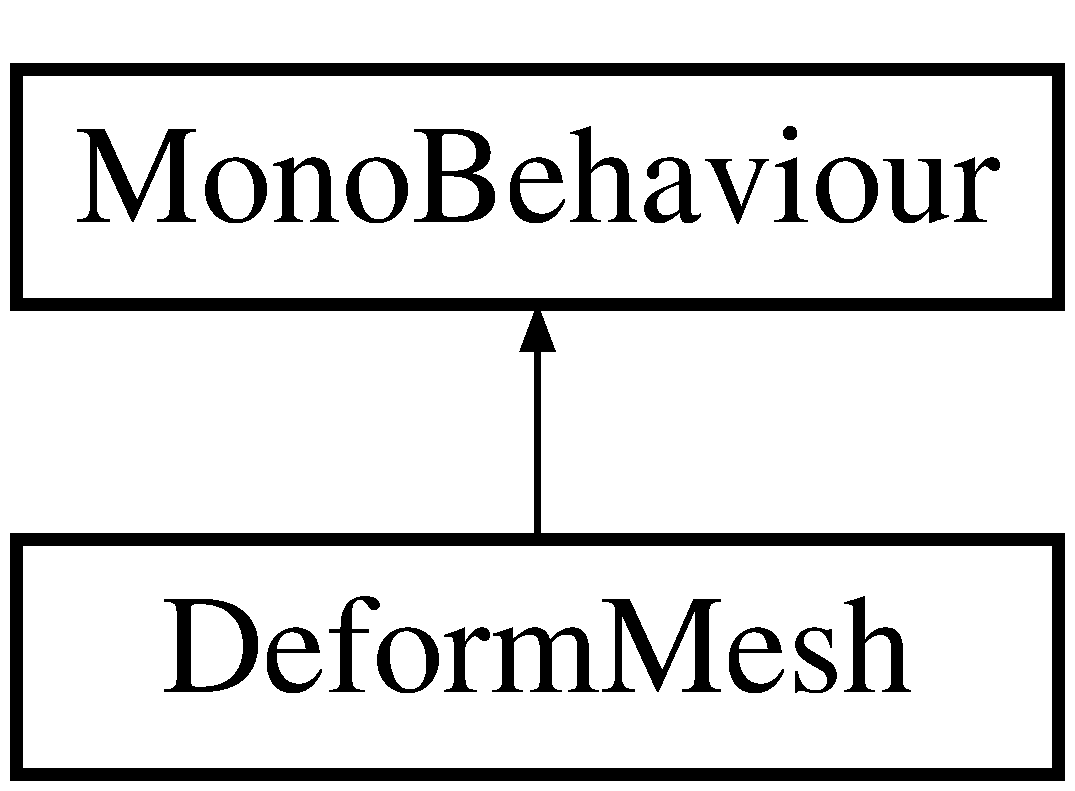
\includegraphics[height=2.000000cm]{class_deform_mesh}
\end{center}
\end{figure}
\subsection*{Public Member Functions}
\begin{DoxyCompactItemize}
\item 
void \hyperlink{class_deform_mesh_ad2caad01ccc1f4bb7331ca536bff0ead}{deform} ()
\begin{DoxyCompactList}\small\item\em Verformt das Mesh, auf dem dieses Script ist, indem alle Vertices in zufällige Richtungen verschoben werden. Zusätzlich wird noch die Farbe verändert \end{DoxyCompactList}\end{DoxyCompactItemize}
\subsection*{Public Attributes}
\begin{DoxyCompactItemize}
\item 
\mbox{\Hypertarget{class_deform_mesh_a8a14edf142b7aaab8b8bc939d987dbe5}\label{class_deform_mesh_a8a14edf142b7aaab8b8bc939d987dbe5}} 
bool {\bfseries deform\+\_\+on\+\_\+awake} = false
\item 
\mbox{\Hypertarget{class_deform_mesh_a4c5e2d7a229657017f4f9eb18fe8425f}\label{class_deform_mesh_a4c5e2d7a229657017f4f9eb18fe8425f}} 
float {\bfseries deform\+\_\+factor}
\item 
\mbox{\Hypertarget{class_deform_mesh_a465d3863ac58c5efc13295f25e952b39}\label{class_deform_mesh_a465d3863ac58c5efc13295f25e952b39}} 
bool {\bfseries change\+\_\+color} = true
\end{DoxyCompactItemize}


\subsection{Member Function Documentation}
\mbox{\Hypertarget{class_deform_mesh_ad2caad01ccc1f4bb7331ca536bff0ead}\label{class_deform_mesh_ad2caad01ccc1f4bb7331ca536bff0ead}} 
\index{Deform\+Mesh@{Deform\+Mesh}!deform@{deform}}
\index{deform@{deform}!Deform\+Mesh@{Deform\+Mesh}}
\subsubsection{\texorpdfstring{deform()}{deform()}}
{\footnotesize\ttfamily void Deform\+Mesh.\+deform (\begin{DoxyParamCaption}{ }\end{DoxyParamCaption})}



Verformt das Mesh, auf dem dieses Script ist, indem alle Vertices in zufällige Richtungen verschoben werden. Zusätzlich wird noch die Farbe verändert 



The documentation for this class was generated from the following file\+:\begin{DoxyCompactItemize}
\item 
/\+Users/\+Leonard/\+Desktop/\+Stor\+Trok/\+Stor Trok/\+Assets/\+Stor Trok/\+Scripts/Deform\+Mesh.\+cs\end{DoxyCompactItemize}

\hypertarget{class_destroyable_object}{}\section{Destroyable\+Object Class Reference}
\label{class_destroyable_object}\index{Destroyable\+Object@{Destroyable\+Object}}
Inheritance diagram for Destroyable\+Object\+:\begin{figure}[H]
\begin{center}
\leavevmode
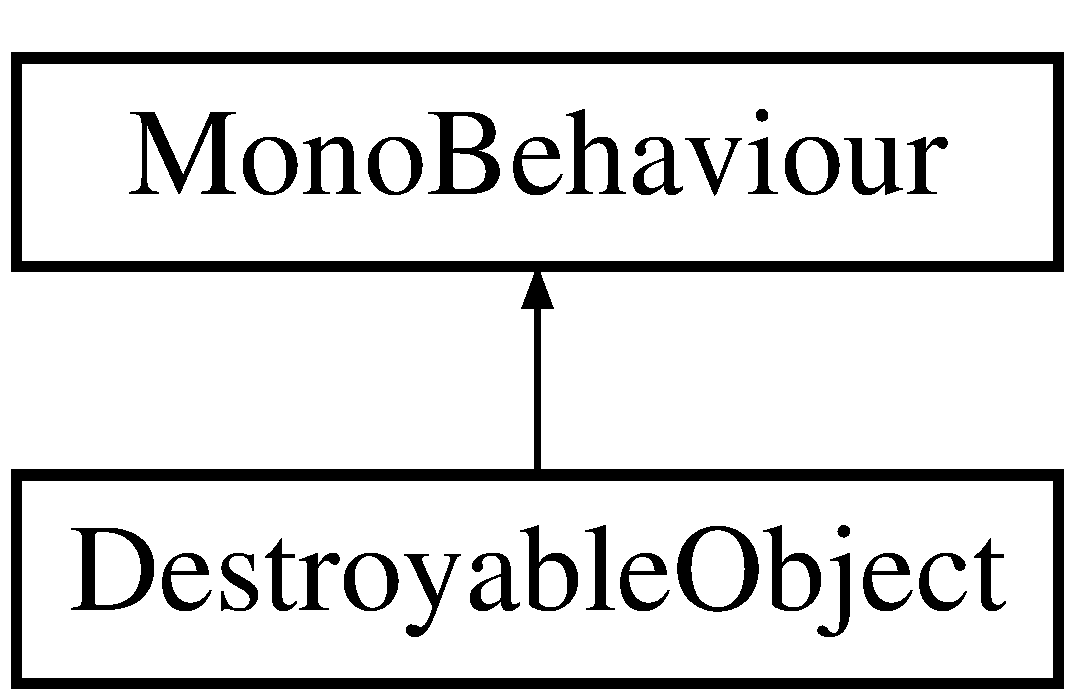
\includegraphics[height=2.000000cm]{class_destroyable_object}
\end{center}
\end{figure}
\subsection*{Public Member Functions}
\begin{DoxyCompactItemize}
\item 
\mbox{\Hypertarget{class_destroyable_object_a18522b00f4ba5ace130a27752cb842df}\label{class_destroyable_object_a18522b00f4ba5ace130a27752cb842df}} 
void {\bfseries destroy} ()
\item 
\mbox{\Hypertarget{class_destroyable_object_a17c15ce3f9d38fe25f62345ebff08966}\label{class_destroyable_object_a17c15ce3f9d38fe25f62345ebff08966}} 
void {\bfseries apply\+\_\+damage} (float dmg)
\end{DoxyCompactItemize}
\subsection*{Static Public Member Functions}
\begin{DoxyCompactItemize}
\item 
\mbox{\Hypertarget{class_destroyable_object_a876de137a9b1a1cb9c16ada789dc42e0}\label{class_destroyable_object_a876de137a9b1a1cb9c16ada789dc42e0}} 
static \hyperlink{class_destroyable_object}{Destroyable\+Object} {\bfseries get\+\_\+destroyable\+\_\+object} (Game\+Object o)
\item 
\mbox{\Hypertarget{class_destroyable_object_ab37ab82ad45036e0d35e6ae6b4e18d97}\label{class_destroyable_object_ab37ab82ad45036e0d35e6ae6b4e18d97}} 
static List$<$ \hyperlink{class_destroyable_object}{Destroyable\+Object} $>$ {\bfseries get\+\_\+active\+\_\+objects} (Object\+Group\+Type type)
\end{DoxyCompactItemize}
\subsection*{Public Attributes}
\begin{DoxyCompactItemize}
\item 
\mbox{\Hypertarget{class_destroyable_object_a133297e2d60dd4d607f75207c55915fa}\label{class_destroyable_object_a133297e2d60dd4d607f75207c55915fa}} 
new string {\bfseries name}
\item 
\mbox{\Hypertarget{class_destroyable_object_a42cd5aea015fb40be1ba3636aeacb3fb}\label{class_destroyable_object_a42cd5aea015fb40be1ba3636aeacb3fb}} 
float {\bfseries max\+\_\+hitpoints}
\item 
\mbox{\Hypertarget{class_destroyable_object_a0a4bb4823dc5a4267f7cf26e6c0a58bf}\label{class_destroyable_object_a0a4bb4823dc5a4267f7cf26e6c0a58bf}} 
float {\bfseries hitpoints}
\item 
\mbox{\Hypertarget{class_destroyable_object_a9b3fb16504b02e723e8707b08b4f795b}\label{class_destroyable_object_a9b3fb16504b02e723e8707b08b4f795b}} 
Object\+Group\+Type {\bfseries object\+\_\+group\+\_\+type}
\item 
\mbox{\Hypertarget{class_destroyable_object_a4c7e19b87151f879ca10fe6a4b1672ce}\label{class_destroyable_object_a4c7e19b87151f879ca10fe6a4b1672ce}} 
bool {\bfseries minimap\+\_\+icon\+\_\+created} = false
\item 
\mbox{\Hypertarget{class_destroyable_object_a1430ab60ae41d40d322dca94cebec995}\label{class_destroyable_object_a1430ab60ae41d40d322dca94cebec995}} 
bool {\bfseries destroyed} = false
\end{DoxyCompactItemize}
\subsection*{Static Public Attributes}
\begin{DoxyCompactItemize}
\item 
\mbox{\Hypertarget{class_destroyable_object_a84ee5e7f255ba1674d29add32ef8cc9a}\label{class_destroyable_object_a84ee5e7f255ba1674d29add32ef8cc9a}} 
static List$<$ \hyperlink{class_destroyable_object}{Destroyable\+Object} $>$ {\bfseries active\+\_\+destroyable\+\_\+objects} = new List$<$\hyperlink{class_destroyable_object}{Destroyable\+Object}$>$()
\end{DoxyCompactItemize}


The documentation for this class was generated from the following file\+:\begin{DoxyCompactItemize}
\item 
/\+Users/\+Leonard/\+Desktop/\+Stor\+Trok/\+Stor Trok/\+Assets/\+Stor Trok/\+Scripts/Destroyable\+Object.\+cs\end{DoxyCompactItemize}

\hypertarget{class_drop}{}\section{Drop Class Reference}
\label{class_drop}\index{Drop@{Drop}}
Inheritance diagram for Drop\+:\begin{figure}[H]
\begin{center}
\leavevmode
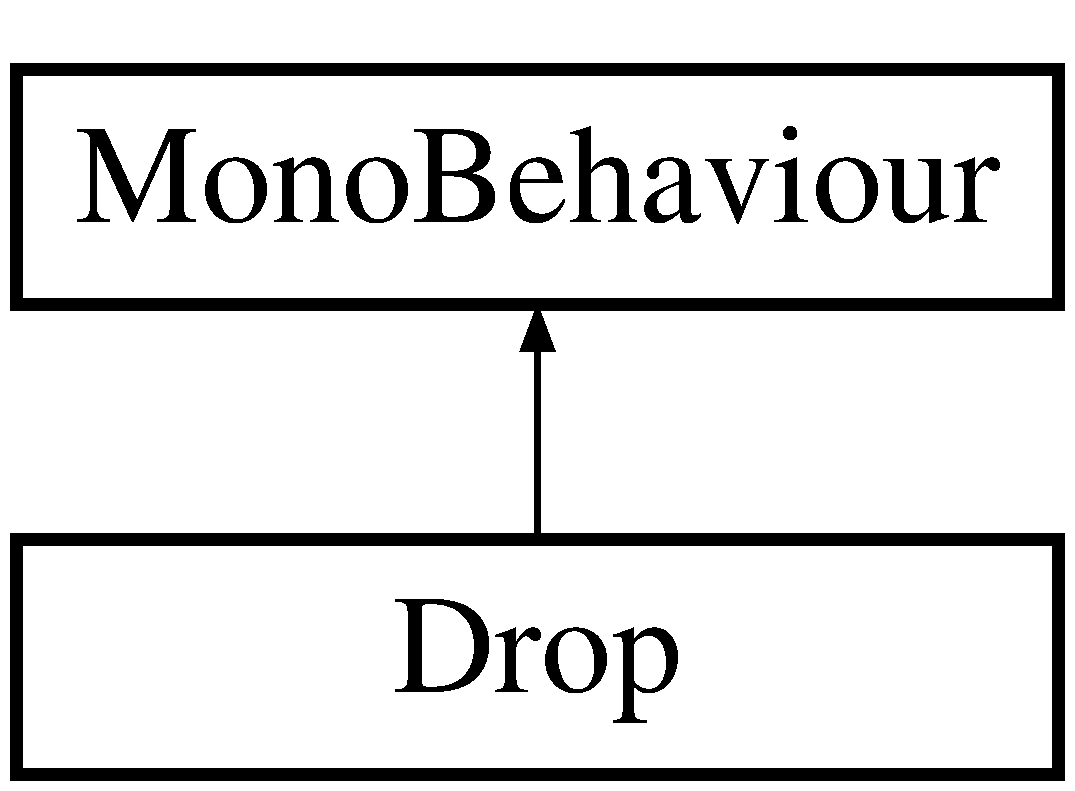
\includegraphics[height=2.000000cm]{class_drop}
\end{center}
\end{figure}
\subsection*{Static Public Member Functions}
\begin{DoxyCompactItemize}
\item 
\mbox{\Hypertarget{class_drop_a14fe640c538e6222553a62fcffc3a5b5}\label{class_drop_a14fe640c538e6222553a62fcffc3a5b5}} 
static void {\bfseries drop\+\_\+item} (Vector3 spawn\+\_\+loc)
\item 
\mbox{\Hypertarget{class_drop_a54be66c04e5bc3cf54e5e1d66f5c819f}\label{class_drop_a54be66c04e5bc3cf54e5e1d66f5c819f}} 
static void {\bfseries drop\+\_\+item} (Vector3 spawn\+\_\+loc, \hyperlink{class_item}{Item} item)
\end{DoxyCompactItemize}
\subsection*{Properties}
\begin{DoxyCompactItemize}
\item 
\mbox{\Hypertarget{class_drop_a05a88f2eb8504a72d7f0ff27bec854b7}\label{class_drop_a05a88f2eb8504a72d7f0ff27bec854b7}} 
\hyperlink{class_item}{Item} {\bfseries item}\hspace{0.3cm}{\ttfamily  \mbox{[}get, set\mbox{]}}
\end{DoxyCompactItemize}


The documentation for this class was generated from the following file\+:\begin{DoxyCompactItemize}
\item 
/\+Users/\+Leonard/\+Desktop/\+Stor\+Trok/\+Stor Trok/\+Assets/\+Stor Trok/\+Scripts/Drop.\+cs\end{DoxyCompactItemize}

\hypertarget{struct_explosion_point}{}\section{Explosion\+Point Struct Reference}
\label{struct_explosion_point}\index{Explosion\+Point@{Explosion\+Point}}
\subsection*{Public Attributes}
\begin{DoxyCompactItemize}
\item 
\mbox{\Hypertarget{struct_explosion_point_a5ea10ad427c367b0d78e8d00d9ae06e9}\label{struct_explosion_point_a5ea10ad427c367b0d78e8d00d9ae06e9}} 
Vector3 {\bfseries point}
\item 
\mbox{\Hypertarget{struct_explosion_point_ac1f32dc2bbf319d64dc1cd31fcc2f5e4}\label{struct_explosion_point_ac1f32dc2bbf319d64dc1cd31fcc2f5e4}} 
float {\bfseries explosion\+\_\+radius}
\end{DoxyCompactItemize}


The documentation for this struct was generated from the following file\+:\begin{DoxyCompactItemize}
\item 
/\+Users/\+Leonard/\+Desktop/\+Stor\+Trok/\+Stor Trok/\+Assets/\+Stor Trok/\+Scripts/\+Spaceship/Schild\+Shader\+Script.\+cs\end{DoxyCompactItemize}

\hypertarget{class_first_person_controller}{}\section{First\+Person\+Controller Class Reference}
\label{class_first_person_controller}\index{First\+Person\+Controller@{First\+Person\+Controller}}
Inheritance diagram for First\+Person\+Controller\+:\begin{figure}[H]
\begin{center}
\leavevmode
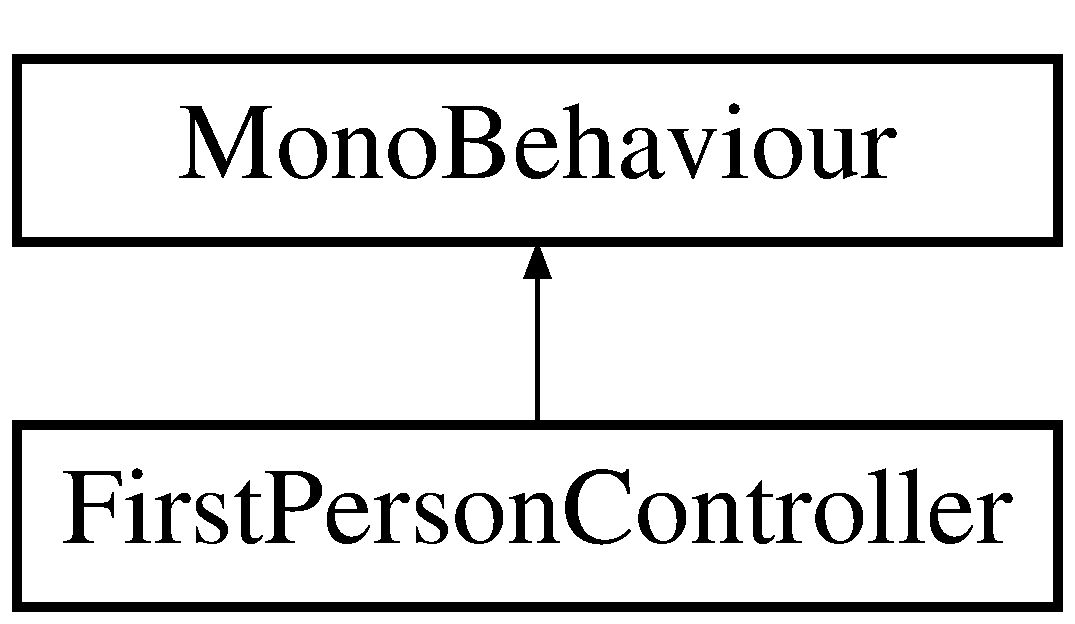
\includegraphics[height=2.000000cm]{class_first_person_controller}
\end{center}
\end{figure}


The documentation for this class was generated from the following file\+:\begin{DoxyCompactItemize}
\item 
/\+Users/\+Leonard/\+Desktop/\+Stor\+Trok/\+Stor Trok/\+Assets/\+Stor Trok/\+Scripts/\+Shop/First\+Person\+Controller.\+cs\end{DoxyCompactItemize}

\hypertarget{class_f_p_controller_v3}{}\section{F\+P\+Controller\+V3 Class Reference}
\label{class_f_p_controller_v3}\index{F\+P\+Controller\+V3@{F\+P\+Controller\+V3}}
Inheritance diagram for F\+P\+Controller\+V3\+:\begin{figure}[H]
\begin{center}
\leavevmode
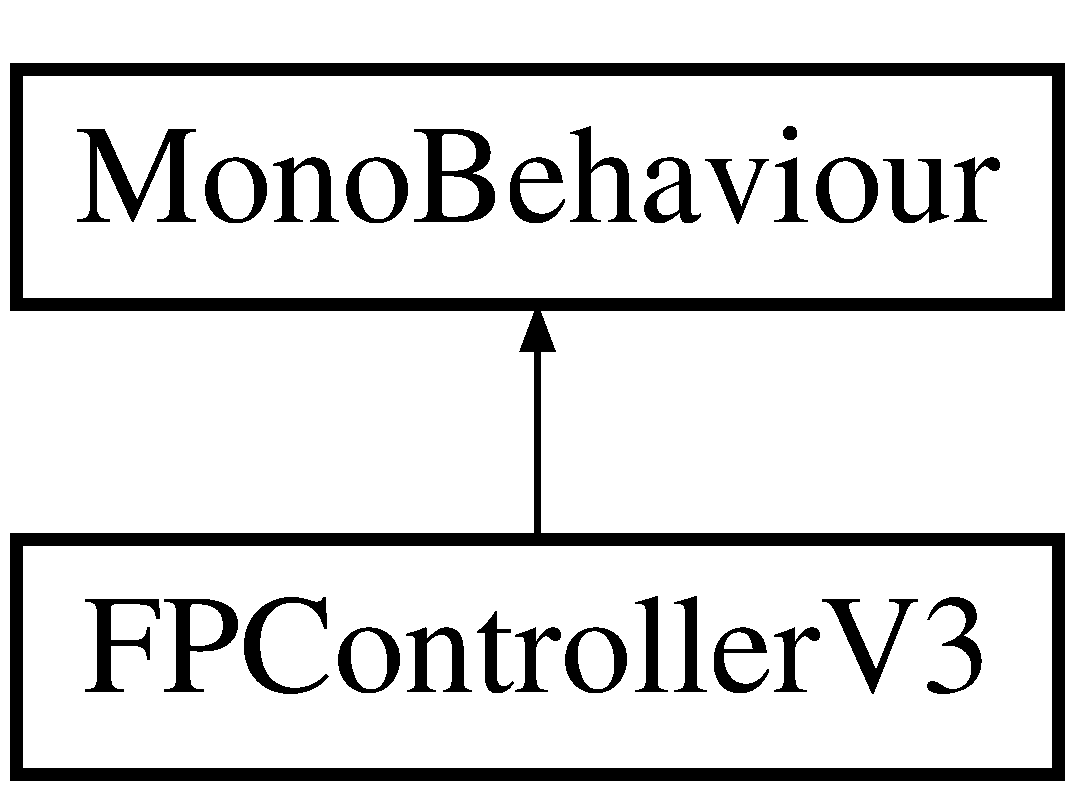
\includegraphics[height=2.000000cm]{class_f_p_controller_v3}
\end{center}
\end{figure}


The documentation for this class was generated from the following file\+:\begin{DoxyCompactItemize}
\item 
/\+Users/\+Leonard/\+Desktop/\+Stor\+Trok/\+Stor Trok/\+Assets/\+Stor Trok/\+Scripts/\+Shop/F\+P\+Controller\+V3.\+cs\end{DoxyCompactItemize}

\hypertarget{class_full_mission}{}\section{Full\+Mission Class Reference}
\label{class_full_mission}\index{Full\+Mission@{Full\+Mission}}
\subsection*{Public Member Functions}
\begin{DoxyCompactItemize}
\item 
\mbox{\Hypertarget{class_full_mission_a5a90a5adac2d2e1316a4874bf1aca86c}\label{class_full_mission_a5a90a5adac2d2e1316a4874bf1aca86c}} 
\hyperlink{class_mission_part}{Mission\+Part} {\bfseries get\+\_\+current\+\_\+mission\+\_\+part} ()
\end{DoxyCompactItemize}
\subsection*{Public Attributes}
\begin{DoxyCompactItemize}
\item 
\mbox{\Hypertarget{class_full_mission_ab5947dac30b18e457de908a355248176}\label{class_full_mission_ab5947dac30b18e457de908a355248176}} 
int {\bfseries ID}
\item 
\mbox{\Hypertarget{class_full_mission_a7907d0de11bfc7527e20b931a6b46749}\label{class_full_mission_a7907d0de11bfc7527e20b931a6b46749}} 
string {\bfseries name}
\item 
\mbox{\Hypertarget{class_full_mission_ace9c96214da769c4233207ac64fb5954}\label{class_full_mission_ace9c96214da769c4233207ac64fb5954}} 
string {\bfseries description}
\item 
\mbox{\Hypertarget{class_full_mission_a534c443b1a75a045823448d0e32b1fee}\label{class_full_mission_a534c443b1a75a045823448d0e32b1fee}} 
int {\bfseries current\+\_\+mission\+\_\+part\+\_\+id}
\item 
\mbox{\Hypertarget{class_full_mission_abef11969217f40de70b464eacaca6433}\label{class_full_mission_abef11969217f40de70b464eacaca6433}} 
List$<$ \hyperlink{class_mission_part}{Mission\+Part} $>$ {\bfseries mission\+\_\+parts}
\end{DoxyCompactItemize}
\subsection*{Properties}
\begin{DoxyCompactItemize}
\item 
\mbox{\Hypertarget{class_full_mission_a298537c804e875cbcb35d1263d8cf61e}\label{class_full_mission_a298537c804e875cbcb35d1263d8cf61e}} 
\hyperlink{class_mission_part}{Mission\+Part} {\bfseries next\+\_\+mission\+\_\+part}\hspace{0.3cm}{\ttfamily  \mbox{[}get\mbox{]}}
\item 
\mbox{\Hypertarget{class_full_mission_a63e47c68aa6392dbcf8c767ca1c91dc0}\label{class_full_mission_a63e47c68aa6392dbcf8c767ca1c91dc0}} 
\hyperlink{class_mission_part}{Mission\+Part} {\bfseries first\+\_\+mission\+\_\+part}\hspace{0.3cm}{\ttfamily  \mbox{[}get\mbox{]}}
\item 
\mbox{\Hypertarget{class_full_mission_a90519c731c203edb8cf794f4f65f90e6}\label{class_full_mission_a90519c731c203edb8cf794f4f65f90e6}} 
\hyperlink{class_mission_part}{Mission\+Part} {\bfseries last\+\_\+mission\+\_\+part}\hspace{0.3cm}{\ttfamily  \mbox{[}get\mbox{]}}
\end{DoxyCompactItemize}


The documentation for this class was generated from the following file\+:\begin{DoxyCompactItemize}
\item 
/\+Users/\+Leonard/\+Desktop/\+Stor\+Trok/\+Stor Trok/\+Assets/\+Stor Trok/\+Scripts/\+Mission/Full\+Mission.\+cs\end{DoxyCompactItemize}

\hypertarget{class_game_preferences}{}\section{Game\+Preferences Class Reference}
\label{class_game_preferences}\index{Game\+Preferences@{Game\+Preferences}}
\subsection*{Static Public Member Functions}
\begin{DoxyCompactItemize}
\item 
\mbox{\Hypertarget{class_game_preferences_ab06a1e41cf247e1ee821a3ecc00c4179}\label{class_game_preferences_ab06a1e41cf247e1ee821a3ecc00c4179}} 
static void {\bfseries save} ()
\item 
\mbox{\Hypertarget{class_game_preferences_a61d1ed4afb240764f1433a32a414683d}\label{class_game_preferences_a61d1ed4afb240764f1433a32a414683d}} 
static void {\bfseries load} ()
\end{DoxyCompactItemize}
\subsection*{Public Attributes}
\begin{DoxyCompactItemize}
\item 
\mbox{\Hypertarget{class_game_preferences_a01d4f79d3433928531bf92fb5c5037b2}\label{class_game_preferences_a01d4f79d3433928531bf92fb5c5037b2}} 
string {\bfseries last\+\_\+username}
\end{DoxyCompactItemize}
\subsection*{Static Public Attributes}
\begin{DoxyCompactItemize}
\item 
\mbox{\Hypertarget{class_game_preferences_a1e0d0f1a45a89ceb7889f38d96e4c104}\label{class_game_preferences_a1e0d0f1a45a89ceb7889f38d96e4c104}} 
static \hyperlink{class_game_preferences}{Game\+Preferences} {\bfseries game\+\_\+preferences}
\end{DoxyCompactItemize}


The documentation for this class was generated from the following file\+:\begin{DoxyCompactItemize}
\item 
/\+Users/\+Leonard/\+Desktop/\+Stor\+Trok/\+Stor Trok/\+Assets/\+Stor Trok/\+Scripts/\+Data/Game\+Preferences.\+cs\end{DoxyCompactItemize}

\hypertarget{class_grid}{}\section{Grid Class Reference}
\label{class_grid}\index{Grid@{Grid}}
Inheritance diagram for Grid\+:\begin{figure}[H]
\begin{center}
\leavevmode
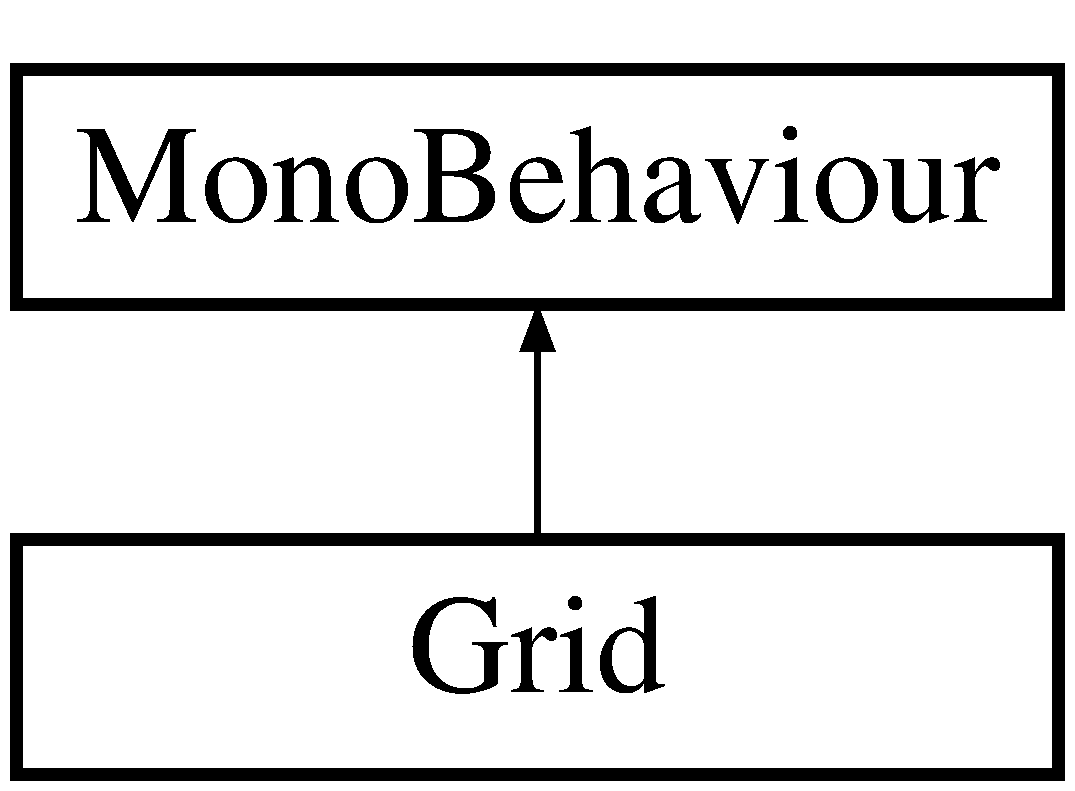
\includegraphics[height=2.000000cm]{class_grid}
\end{center}
\end{figure}
\subsection*{Public Attributes}
\begin{DoxyCompactItemize}
\item 
\mbox{\Hypertarget{class_grid_adae5c3aff7bef22c94ead5886b01f7c1}\label{class_grid_adae5c3aff7bef22c94ead5886b01f7c1}} 
float {\bfseries tile\+\_\+size} = 10
\item 
\mbox{\Hypertarget{class_grid_a9fdf4a2c1386a1fc9ece1ae594054ed6}\label{class_grid_a9fdf4a2c1386a1fc9ece1ae594054ed6}} 
Material {\bfseries grid\+\_\+material}
\end{DoxyCompactItemize}


The documentation for this class was generated from the following file\+:\begin{DoxyCompactItemize}
\item 
/\+Users/\+Leonard/\+Desktop/\+Stor\+Trok/\+Stor Trok/\+Assets/\+Stor Trok/\+Scripts/\+Tests/Grid.\+cs\end{DoxyCompactItemize}

\hypertarget{class_impuls_antrieb}{}\section{Impuls\+Antrieb Class Reference}
\label{class_impuls_antrieb}\index{Impuls\+Antrieb@{Impuls\+Antrieb}}
Inheritance diagram for Impuls\+Antrieb\+:\begin{figure}[H]
\begin{center}
\leavevmode
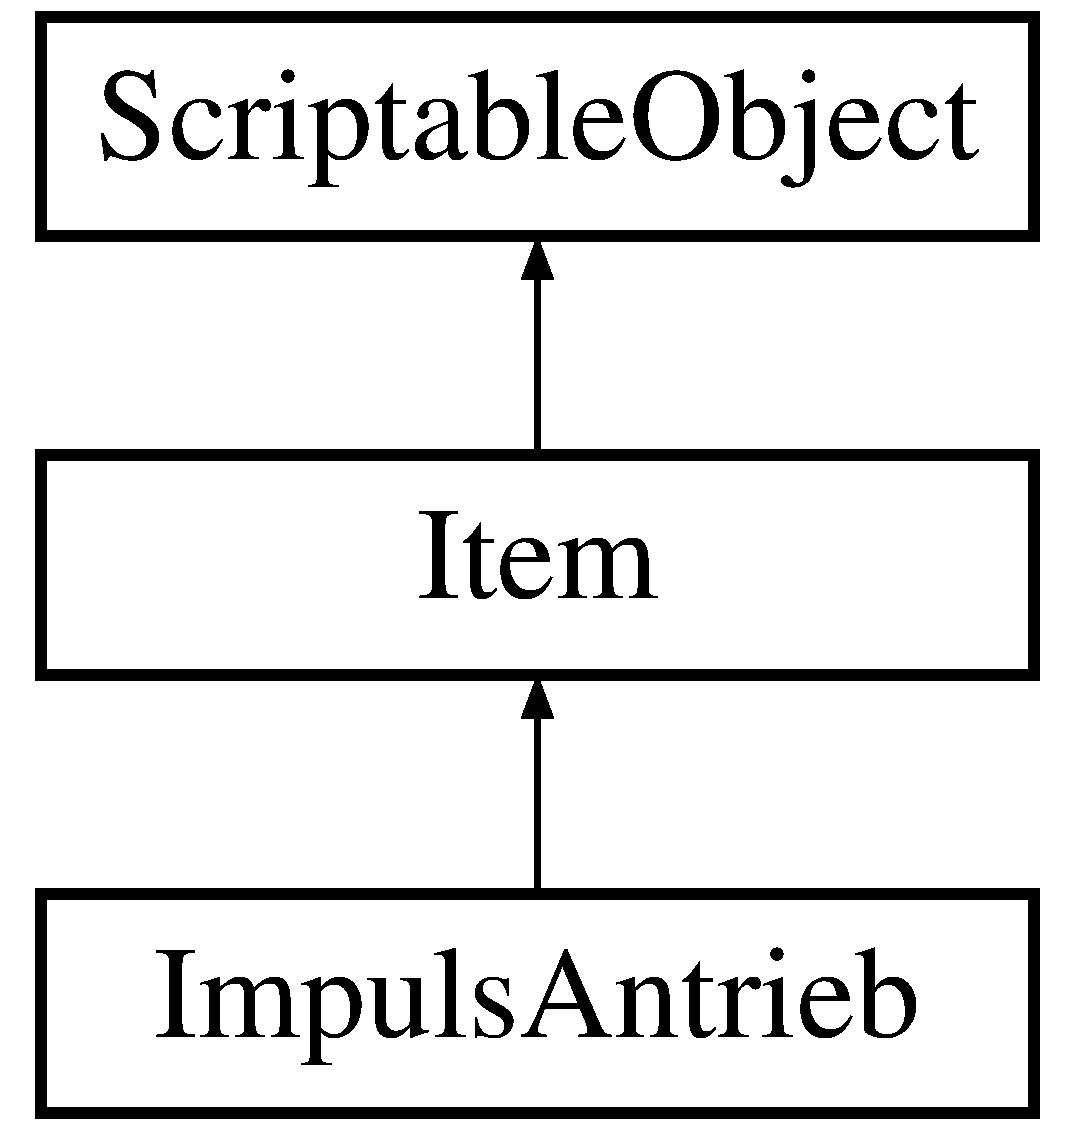
\includegraphics[height=3.000000cm]{class_impuls_antrieb}
\end{center}
\end{figure}
\subsection*{Public Member Functions}
\begin{DoxyCompactItemize}
\item 
override string \hyperlink{class_impuls_antrieb_ad9c1cf88503eecd20366493ac6f6b855}{get\+\_\+description\+\_\+text} ()
\begin{DoxyCompactList}\small\item\em Erstellt einen Text, der im \hyperlink{class_inventar}{Inventar} angezeigt wird, wenn der Mauszeiger auf dem \hyperlink{class_item}{Item} ist \end{DoxyCompactList}\end{DoxyCompactItemize}
\subsection*{Public Attributes}
\begin{DoxyCompactItemize}
\item 
\mbox{\Hypertarget{class_impuls_antrieb_a70ddf69ae8d2105f7a0720a0d58c15e4}\label{class_impuls_antrieb_a70ddf69ae8d2105f7a0720a0d58c15e4}} 
float {\bfseries max\+\_\+speed}
\end{DoxyCompactItemize}
\subsection*{Additional Inherited Members}


\subsection{Member Function Documentation}
\mbox{\Hypertarget{class_impuls_antrieb_ad9c1cf88503eecd20366493ac6f6b855}\label{class_impuls_antrieb_ad9c1cf88503eecd20366493ac6f6b855}} 
\index{Impuls\+Antrieb@{Impuls\+Antrieb}!get\+\_\+description\+\_\+text@{get\+\_\+description\+\_\+text}}
\index{get\+\_\+description\+\_\+text@{get\+\_\+description\+\_\+text}!Impuls\+Antrieb@{Impuls\+Antrieb}}
\subsubsection{\texorpdfstring{get\+\_\+description\+\_\+text()}{get\_description\_text()}}
{\footnotesize\ttfamily override string Impuls\+Antrieb.\+get\+\_\+description\+\_\+text (\begin{DoxyParamCaption}{ }\end{DoxyParamCaption})\hspace{0.3cm}{\ttfamily [virtual]}}



Erstellt einen Text, der im \hyperlink{class_inventar}{Inventar} angezeigt wird, wenn der Mauszeiger auf dem \hyperlink{class_item}{Item} ist 

\begin{DoxyReturn}{Returns}
The description text.
\end{DoxyReturn}


Implements \hyperlink{class_item_ab868f8ccad92378f7352e3a9e0f755ff}{Item}.



The documentation for this class was generated from the following file\+:\begin{DoxyCompactItemize}
\item 
/\+Users/\+Leonard/\+Desktop/\+Stor\+Trok/\+Stor Trok/\+Assets/\+Stor Trok/\+Scripts/\+Items/Impuls\+Antrieb.\+cs\end{DoxyCompactItemize}

\hypertarget{class_interactive_message}{}\section{Interactive\+Message Class Reference}
\label{class_interactive_message}\index{Interactive\+Message@{Interactive\+Message}}
Inheritance diagram for Interactive\+Message\+:\begin{figure}[H]
\begin{center}
\leavevmode
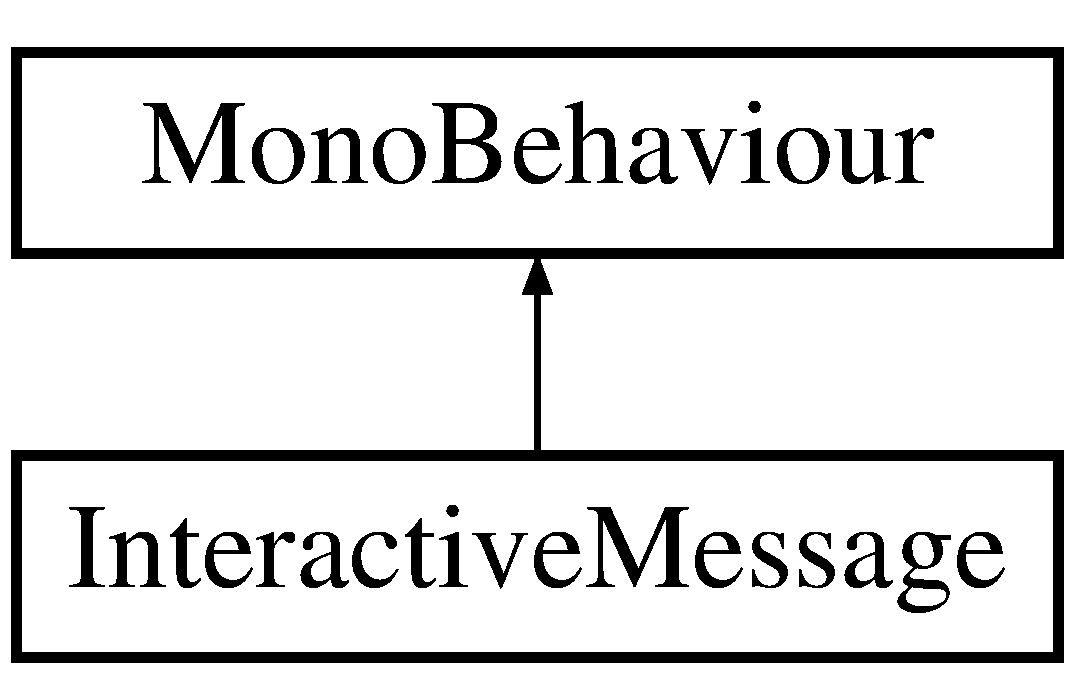
\includegraphics[height=2.000000cm]{class_interactive_message}
\end{center}
\end{figure}
\subsection*{Public Member Functions}
\begin{DoxyCompactItemize}
\item 
\mbox{\Hypertarget{class_interactive_message_a1fb9f1b10aed28d30c3460faab2675b1}\label{class_interactive_message_a1fb9f1b10aed28d30c3460faab2675b1}} 
void {\bfseries remove\+\_\+button} (\hyperlink{class_interactive_message_button}{Interactive\+Message\+Button} btn)
\item 
\mbox{\Hypertarget{class_interactive_message_a79614aef5ec800f9328e607c4f5ebcbb}\label{class_interactive_message_a79614aef5ec800f9328e607c4f5ebcbb}} 
void {\bfseries enable} (Interactive\+Message\+Content\+Type type)
\item 
\mbox{\Hypertarget{class_interactive_message_a1d8149d96b59c4034419733ecf35d537}\label{class_interactive_message_a1d8149d96b59c4034419733ecf35d537}} 
void {\bfseries button\+\_\+clicked} (int button\+\_\+number)
\end{DoxyCompactItemize}
\subsection*{Public Attributes}
\begin{DoxyCompactItemize}
\item 
\mbox{\Hypertarget{class_interactive_message_ae5c09ea48c335dd92bc294118a140c95}\label{class_interactive_message_ae5c09ea48c335dd92bc294118a140c95}} 
Text {\bfseries description\+\_\+text}
\item 
\mbox{\Hypertarget{class_interactive_message_a9b28331618a1eb7e15e897b87e8ecd61}\label{class_interactive_message_a9b28331618a1eb7e15e897b87e8ecd61}} 
List$<$ \hyperlink{class_interactive_message_button}{Interactive\+Message\+Button} $>$ {\bfseries buttons} = new List$<$\hyperlink{class_interactive_message_button}{Interactive\+Message\+Button}$>$()
\item 
\mbox{\Hypertarget{class_interactive_message_a2c49d0ae14831a0ff25c8576c4b960fb}\label{class_interactive_message_a2c49d0ae14831a0ff25c8576c4b960fb}} 
Game\+Object {\bfseries image}
\end{DoxyCompactItemize}


The documentation for this class was generated from the following file\+:\begin{DoxyCompactItemize}
\item 
/\+Users/\+Leonard/\+Desktop/\+Stor\+Trok/\+Stor Trok/\+Assets/\+Stor Trok/\+Scripts/\+U\+I/Interactive\+Message.\+cs\end{DoxyCompactItemize}

\hypertarget{class_interactive_message_button}{}\section{Interactive\+Message\+Button Class Reference}
\label{class_interactive_message_button}\index{Interactive\+Message\+Button@{Interactive\+Message\+Button}}
\subsection*{Public Attributes}
\begin{DoxyCompactItemize}
\item 
\mbox{\Hypertarget{class_interactive_message_button_acff0bcb6a248f2328cd6fe94eb11879c}\label{class_interactive_message_button_acff0bcb6a248f2328cd6fe94eb11879c}} 
Interactive\+Message\+Content\+Type {\bfseries content\+\_\+type}
\item 
\mbox{\Hypertarget{class_interactive_message_button_a8148af4974fa552f7f7a9bf99a782814}\label{class_interactive_message_button_a8148af4974fa552f7f7a9bf99a782814}} 
string {\bfseries description\+\_\+text}
\item 
\mbox{\Hypertarget{class_interactive_message_button_a4824df2f4f364ca8c6e1d252e15bb421}\label{class_interactive_message_button_a4824df2f4f364ca8c6e1d252e15bb421}} 
Button {\bfseries button}
\item 
\mbox{\Hypertarget{class_interactive_message_button_acbe1c2b46e1c7cfa13da6dfb99691942}\label{class_interactive_message_button_acbe1c2b46e1c7cfa13da6dfb99691942}} 
Text {\bfseries button\+\_\+text}
\item 
\mbox{\Hypertarget{class_interactive_message_button_a78e912d4a9ab380f32b25d4e072d8946}\label{class_interactive_message_button_a78e912d4a9ab380f32b25d4e072d8946}} 
\hyperlink{class_drop}{Drop} {\bfseries drop}
\item 
\mbox{\Hypertarget{class_interactive_message_button_afa150ab79d07570f62e1d46a3df3ba8d}\label{class_interactive_message_button_afa150ab79d07570f62e1d46a3df3ba8d}} 
bool {\bfseries is\+\_\+mission} = false
\end{DoxyCompactItemize}


The documentation for this class was generated from the following file\+:\begin{DoxyCompactItemize}
\item 
/\+Users/\+Leonard/\+Desktop/\+Stor\+Trok/\+Stor Trok/\+Assets/\+Stor Trok/\+Scripts/\+U\+I/Interactive\+Message.\+cs\end{DoxyCompactItemize}

\hypertarget{class_inventar}{}\section{Inventar Class Reference}
\label{class_inventar}\index{Inventar@{Inventar}}
\subsection*{Public Member Functions}
\begin{DoxyCompactItemize}
\item 
\mbox{\Hypertarget{class_inventar_a6958a3e3958f2e8cdcbaeeda9999c100}\label{class_inventar_a6958a3e3958f2e8cdcbaeeda9999c100}} 
bool {\bfseries add\+\_\+item} (\hyperlink{class_item}{Item} item)
\item 
\mbox{\Hypertarget{class_inventar_a56116859c3721894aa5b93d4c3dfd7ca}\label{class_inventar_a56116859c3721894aa5b93d4c3dfd7ca}} 
bool {\bfseries add\+\_\+item} (\hyperlink{class_item}{Item} item, int index)
\end{DoxyCompactItemize}
\subsection*{Public Attributes}
\begin{DoxyCompactItemize}
\item 
\mbox{\Hypertarget{class_inventar_a052494e4e79676f4e4b76d2667146357}\label{class_inventar_a052494e4e79676f4e4b76d2667146357}} 
\hyperlink{class_item}{Item} \mbox{[}$\,$\mbox{]} {\bfseries items}
\item 
\mbox{\Hypertarget{class_inventar_ab1393d898b97709b67eb7376daa37913}\label{class_inventar_ab1393d898b97709b67eb7376daa37913}} 
int {\bfseries capacity} = 16
\end{DoxyCompactItemize}


The documentation for this class was generated from the following file\+:\begin{DoxyCompactItemize}
\item 
/\+Users/\+Leonard/\+Desktop/\+Stor\+Trok/\+Stor Trok/\+Assets/\+Stor Trok/\+Scripts/\+Player/Inventar.\+cs\end{DoxyCompactItemize}

\hypertarget{class_inventory}{}\section{Inventory Class Reference}
\label{class_inventory}\index{Inventory@{Inventory}}
Inheritance diagram for Inventory\+:\begin{figure}[H]
\begin{center}
\leavevmode
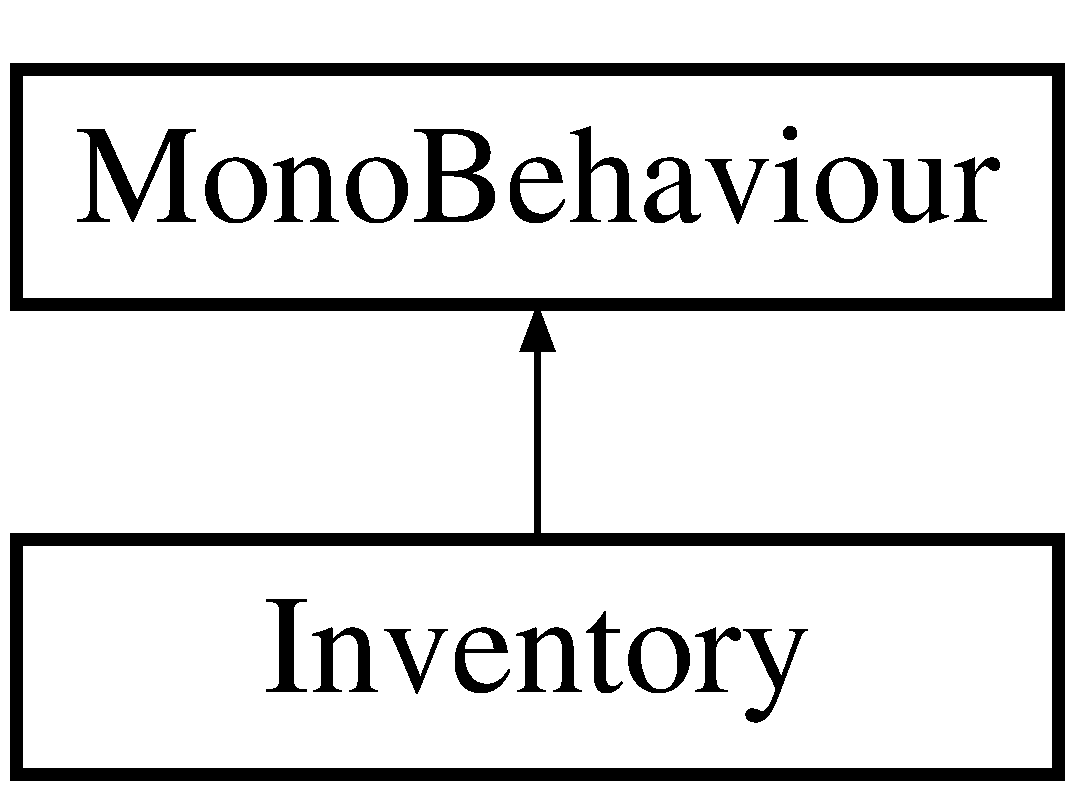
\includegraphics[height=2.000000cm]{class_inventory}
\end{center}
\end{figure}
\subsection*{Public Member Functions}
\begin{DoxyCompactItemize}
\item 
\mbox{\Hypertarget{class_inventory_afbb4b8ba992ef57b5760e661a67b3a44}\label{class_inventory_afbb4b8ba992ef57b5760e661a67b3a44}} 
void {\bfseries set\+\_\+buttons} ()
\end{DoxyCompactItemize}
\subsection*{Public Attributes}
\begin{DoxyCompactItemize}
\item 
\mbox{\Hypertarget{class_inventory_a21c56ad3fd9f538ef95afd49e5a5872d}\label{class_inventory_a21c56ad3fd9f538ef95afd49e5a5872d}} 
int {\bfseries rows} = 6
\item 
\mbox{\Hypertarget{class_inventory_ae2c651436e459d9eb1965af0f3dfedaa}\label{class_inventory_ae2c651436e459d9eb1965af0f3dfedaa}} 
int {\bfseries columns} = 4
\item 
\mbox{\Hypertarget{class_inventory_a48805ee96166b00a3ba16885f07064c6}\label{class_inventory_a48805ee96166b00a3ba16885f07064c6}} 
Game\+Object {\bfseries item\+\_\+button}
\item 
\mbox{\Hypertarget{class_inventory_a54ca888fe8cda256797d7c0522291880}\label{class_inventory_a54ca888fe8cda256797d7c0522291880}} 
List$<$ Game\+Object $>$ {\bfseries item\+\_\+buttons}
\end{DoxyCompactItemize}
\subsection*{Static Public Attributes}
\begin{DoxyCompactItemize}
\item 
\mbox{\Hypertarget{class_inventory_a8d51956ba6315eed2c72528ef9b806b6}\label{class_inventory_a8d51956ba6315eed2c72528ef9b806b6}} 
static \hyperlink{class_inventory}{Inventory} {\bfseries inventory}
\end{DoxyCompactItemize}


The documentation for this class was generated from the following file\+:\begin{DoxyCompactItemize}
\item 
/\+Users/\+Leonard/\+Desktop/\+Stor\+Trok/\+Stor Trok/\+Assets/\+Stor Trok/\+Scripts/\+U\+I/\+Inventory/Inventory.\+cs\end{DoxyCompactItemize}

\hypertarget{class_item}{}\section{Item Class Reference}
\label{class_item}\index{Item@{Item}}
Inheritance diagram for Item\+:\begin{figure}[H]
\begin{center}
\leavevmode
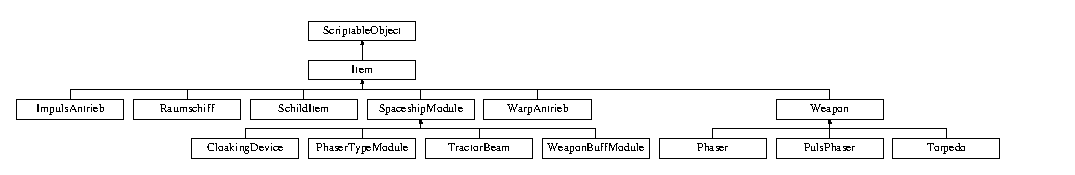
\includegraphics[height=1.899915cm]{class_item}
\end{center}
\end{figure}
\subsection*{Public Member Functions}
\begin{DoxyCompactItemize}
\item 
abstract string \hyperlink{class_item_ab868f8ccad92378f7352e3a9e0f755ff}{get\+\_\+description\+\_\+text} ()
\begin{DoxyCompactList}\small\item\em Erstellt einen Text, der im \hyperlink{class_inventar}{Inventar} angezeigt wird, wenn der Mauszeiger auf dem \hyperlink{class_item}{Item} ist \end{DoxyCompactList}\end{DoxyCompactItemize}
\subsection*{Static Public Member Functions}
\begin{DoxyCompactItemize}
\item 
\mbox{\Hypertarget{class_item_a397f3378e09c0c3e2b7552376770a8ed}\label{class_item_a397f3378e09c0c3e2b7552376770a8ed}} 
static \hyperlink{class_item}{Item} {\bfseries get\+\_\+item\+\_\+at\+\_\+position\+\_\+in\+\_\+list} (int index)
\item 
static \hyperlink{class_item}{Item} \hyperlink{class_item_a434d366123e8cde420cd08d6d55cf2e2}{get\+\_\+item\+\_\+by\+\_\+id} (int id)
\begin{DoxyCompactList}\small\item\em Findet ein \hyperlink{class_item}{Item} per ID und gibt eine Kopie dessen zurück. \end{DoxyCompactList}\item 
static void \hyperlink{class_item_abb13a205923316049fa1854b954a55a0}{load\+\_\+items} ()
\begin{DoxyCompactList}\small\item\em Lädt die Item-\/\+Daten aus dem Resource-\/\+Folder \end{DoxyCompactList}\item 
static \hyperlink{class_item}{Item} \hyperlink{class_item_a6728fc973c3b5a55a14fcfe8c65c541c}{random} ()
\begin{DoxyCompactList}\small\item\em Wählt ein zufälliges \hyperlink{class_item}{Item} aus \end{DoxyCompactList}\end{DoxyCompactItemize}
\subsection*{Public Attributes}
\begin{DoxyCompactItemize}
\item 
int \hyperlink{class_item_a9bb8b7d4f5a5a3242136bd49eb2833da}{ID}
\begin{DoxyCompactList}\small\item\em Unique ID für das \hyperlink{class_item}{Item} \end{DoxyCompactList}\item 
Sprite \hyperlink{class_item_a7306d611989cda78275f2c097553b1c1}{inventory\+\_\+tex}
\begin{DoxyCompactList}\small\item\em Das Sprite, das im \hyperlink{class_inventar}{Inventar} für das \hyperlink{class_item}{Item} angezeigt wird \end{DoxyCompactList}\item 
new string \hyperlink{class_item_ad853c3926372e263a546f9a411ef5323}{name}
\begin{DoxyCompactList}\small\item\em Name des Items \end{DoxyCompactList}\item 
int \hyperlink{class_item_a32ee9b922a1369a8fd6447198a987331}{mark\+\_\+number} = 0
\begin{DoxyCompactList}\small\item\em Nummer des Items, z.\+B. \hyperlink{class_phaser}{Phaser} 1 oder \hyperlink{class_torpedo}{Torpedo} 6 \end{DoxyCompactList}\item 
int \hyperlink{class_item_a3be388595e4069403ed40296fe9a104a}{cost}
\begin{DoxyCompactList}\small\item\em Preis des Items \end{DoxyCompactList}\item 
Item\+Type \hyperlink{class_item_a6bb9d607aa6d88c13e82c37e9da08e73}{item\+\_\+type}
\begin{DoxyCompactList}\small\item\em Typ des Items\+: \hyperlink{class_schild}{Schild}, Waffe, etc. \end{DoxyCompactList}\end{DoxyCompactItemize}
\subsection*{Static Public Attributes}
\begin{DoxyCompactItemize}
\item 
\mbox{\Hypertarget{class_item_a123b132e4d6dfc056b81fe5358fe3e0e}\label{class_item_a123b132e4d6dfc056b81fe5358fe3e0e}} 
static List$<$ \hyperlink{class_item}{Item} $>$ {\bfseries All\+Items} = new List$<$\hyperlink{class_item}{Item}$>$ ()
\end{DoxyCompactItemize}


\subsection{Member Function Documentation}
\mbox{\Hypertarget{class_item_ab868f8ccad92378f7352e3a9e0f755ff}\label{class_item_ab868f8ccad92378f7352e3a9e0f755ff}} 
\index{Item@{Item}!get\+\_\+description\+\_\+text@{get\+\_\+description\+\_\+text}}
\index{get\+\_\+description\+\_\+text@{get\+\_\+description\+\_\+text}!Item@{Item}}
\subsubsection{\texorpdfstring{get\+\_\+description\+\_\+text()}{get\_description\_text()}}
{\footnotesize\ttfamily abstract string Item.\+get\+\_\+description\+\_\+text (\begin{DoxyParamCaption}{ }\end{DoxyParamCaption})\hspace{0.3cm}{\ttfamily [pure virtual]}}



Erstellt einen Text, der im \hyperlink{class_inventar}{Inventar} angezeigt wird, wenn der Mauszeiger auf dem \hyperlink{class_item}{Item} ist 

\begin{DoxyReturn}{Returns}
The description text.
\end{DoxyReturn}


Implemented in \hyperlink{class_weapon_a8fcfb4f08ea22a8fc60790770a58b985}{Weapon}, \hyperlink{class_raumschiff_a9aa65a7d3deb846709b85be4d157d621}{Raumschiff}, \hyperlink{class_spaceship_module_a787019cbebc400d17dc7233ca315c6da}{Spaceship\+Module}, \hyperlink{class_warp_antrieb_a6fab9b91e972d0411541b2a2ff89a21e}{Warp\+Antrieb}, \hyperlink{class_schild_item_a6e09e58ec5afc082636c1a9b4b715613}{Schild\+Item}, and \hyperlink{class_impuls_antrieb_ad9c1cf88503eecd20366493ac6f6b855}{Impuls\+Antrieb}.

\mbox{\Hypertarget{class_item_a434d366123e8cde420cd08d6d55cf2e2}\label{class_item_a434d366123e8cde420cd08d6d55cf2e2}} 
\index{Item@{Item}!get\+\_\+item\+\_\+by\+\_\+id@{get\+\_\+item\+\_\+by\+\_\+id}}
\index{get\+\_\+item\+\_\+by\+\_\+id@{get\+\_\+item\+\_\+by\+\_\+id}!Item@{Item}}
\subsubsection{\texorpdfstring{get\+\_\+item\+\_\+by\+\_\+id()}{get\_item\_by\_id()}}
{\footnotesize\ttfamily static \hyperlink{class_item}{Item} Item.\+get\+\_\+item\+\_\+by\+\_\+id (\begin{DoxyParamCaption}\item[{int}]{id }\end{DoxyParamCaption})\hspace{0.3cm}{\ttfamily [static]}}



Findet ein \hyperlink{class_item}{Item} per ID und gibt eine Kopie dessen zurück. 

\begin{DoxyReturn}{Returns}
Kopie des gefundenen Items oder null, wenn kein \hyperlink{class_item}{Item} mit dieser ID existier.
\end{DoxyReturn}

\begin{DoxyParams}{Parameters}
{\em id} & Die ID des zu suchenden Items.\\
\hline
\end{DoxyParams}
\mbox{\Hypertarget{class_item_abb13a205923316049fa1854b954a55a0}\label{class_item_abb13a205923316049fa1854b954a55a0}} 
\index{Item@{Item}!load\+\_\+items@{load\+\_\+items}}
\index{load\+\_\+items@{load\+\_\+items}!Item@{Item}}
\subsubsection{\texorpdfstring{load\+\_\+items()}{load\_items()}}
{\footnotesize\ttfamily static void Item.\+load\+\_\+items (\begin{DoxyParamCaption}{ }\end{DoxyParamCaption})\hspace{0.3cm}{\ttfamily [static]}}



Lädt die Item-\/\+Daten aus dem Resource-\/\+Folder 

\mbox{\Hypertarget{class_item_a6728fc973c3b5a55a14fcfe8c65c541c}\label{class_item_a6728fc973c3b5a55a14fcfe8c65c541c}} 
\index{Item@{Item}!random@{random}}
\index{random@{random}!Item@{Item}}
\subsubsection{\texorpdfstring{random()}{random()}}
{\footnotesize\ttfamily static \hyperlink{class_item}{Item} Item.\+random (\begin{DoxyParamCaption}{ }\end{DoxyParamCaption})\hspace{0.3cm}{\ttfamily [static]}}



Wählt ein zufälliges \hyperlink{class_item}{Item} aus 



\subsection{Member Data Documentation}
\mbox{\Hypertarget{class_item_a3be388595e4069403ed40296fe9a104a}\label{class_item_a3be388595e4069403ed40296fe9a104a}} 
\index{Item@{Item}!cost@{cost}}
\index{cost@{cost}!Item@{Item}}
\subsubsection{\texorpdfstring{cost}{cost}}
{\footnotesize\ttfamily int Item.\+cost}



Preis des Items 

\mbox{\Hypertarget{class_item_a9bb8b7d4f5a5a3242136bd49eb2833da}\label{class_item_a9bb8b7d4f5a5a3242136bd49eb2833da}} 
\index{Item@{Item}!ID@{ID}}
\index{ID@{ID}!Item@{Item}}
\subsubsection{\texorpdfstring{ID}{ID}}
{\footnotesize\ttfamily int Item.\+ID}



Unique ID für das \hyperlink{class_item}{Item} 

\mbox{\Hypertarget{class_item_a7306d611989cda78275f2c097553b1c1}\label{class_item_a7306d611989cda78275f2c097553b1c1}} 
\index{Item@{Item}!inventory\+\_\+tex@{inventory\+\_\+tex}}
\index{inventory\+\_\+tex@{inventory\+\_\+tex}!Item@{Item}}
\subsubsection{\texorpdfstring{inventory\+\_\+tex}{inventory\_tex}}
{\footnotesize\ttfamily Sprite Item.\+inventory\+\_\+tex}



Das Sprite, das im \hyperlink{class_inventar}{Inventar} für das \hyperlink{class_item}{Item} angezeigt wird 

\mbox{\Hypertarget{class_item_a6bb9d607aa6d88c13e82c37e9da08e73}\label{class_item_a6bb9d607aa6d88c13e82c37e9da08e73}} 
\index{Item@{Item}!item\+\_\+type@{item\+\_\+type}}
\index{item\+\_\+type@{item\+\_\+type}!Item@{Item}}
\subsubsection{\texorpdfstring{item\+\_\+type}{item\_type}}
{\footnotesize\ttfamily Item\+Type Item.\+item\+\_\+type}



Typ des Items\+: \hyperlink{class_schild}{Schild}, Waffe, etc. 

\mbox{\Hypertarget{class_item_a32ee9b922a1369a8fd6447198a987331}\label{class_item_a32ee9b922a1369a8fd6447198a987331}} 
\index{Item@{Item}!mark\+\_\+number@{mark\+\_\+number}}
\index{mark\+\_\+number@{mark\+\_\+number}!Item@{Item}}
\subsubsection{\texorpdfstring{mark\+\_\+number}{mark\_number}}
{\footnotesize\ttfamily int Item.\+mark\+\_\+number = 0}



Nummer des Items, z.\+B. \hyperlink{class_phaser}{Phaser} 1 oder \hyperlink{class_torpedo}{Torpedo} 6 

\mbox{\Hypertarget{class_item_ad853c3926372e263a546f9a411ef5323}\label{class_item_ad853c3926372e263a546f9a411ef5323}} 
\index{Item@{Item}!name@{name}}
\index{name@{name}!Item@{Item}}
\subsubsection{\texorpdfstring{name}{name}}
{\footnotesize\ttfamily new string Item.\+name}



Name des Items 



The documentation for this class was generated from the following file\+:\begin{DoxyCompactItemize}
\item 
/\+Users/\+Leonard/\+Desktop/\+Stor\+Trok/\+Stor Trok/\+Assets/\+Stor Trok/\+Scripts/\+Items/Item.\+cs\end{DoxyCompactItemize}

\hypertarget{class_item_button}{}\section{Item\+Button Class Reference}
\label{class_item_button}\index{Item\+Button@{Item\+Button}}
Inheritance diagram for Item\+Button\+:\begin{figure}[H]
\begin{center}
\leavevmode
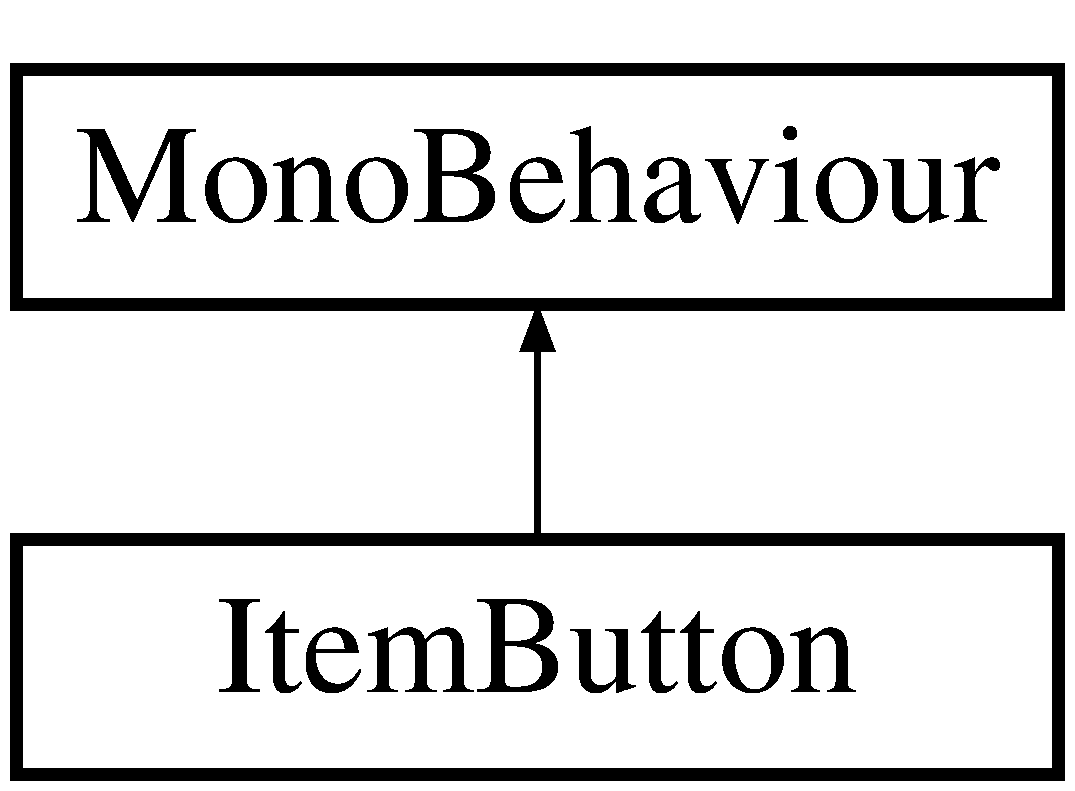
\includegraphics[height=2.000000cm]{class_item_button}
\end{center}
\end{figure}
\subsection*{Public Member Functions}
\begin{DoxyCompactItemize}
\item 
\mbox{\Hypertarget{class_item_button_a5e9b628234f4463b5854f8adcdf1bdcb}\label{class_item_button_a5e9b628234f4463b5854f8adcdf1bdcb}} 
void {\bfseries set\+\_\+item} (\hyperlink{class_item}{Item} i)
\item 
\mbox{\Hypertarget{class_item_button_a89814be3c1f66f34e4d6b4e7af48d263}\label{class_item_button_a89814be3c1f66f34e4d6b4e7af48d263}} 
void {\bfseries pointer\+\_\+enter} ()
\item 
\mbox{\Hypertarget{class_item_button_ab38e5b4a0f9d9b0743e58429db01cb97}\label{class_item_button_ab38e5b4a0f9d9b0743e58429db01cb97}} 
void {\bfseries pointer\+\_\+exit} ()
\item 
\mbox{\Hypertarget{class_item_button_a5d315e5efe5b0f2b1b3ec181bf82f7e4}\label{class_item_button_a5d315e5efe5b0f2b1b3ec181bf82f7e4}} 
void {\bfseries click} ()
\end{DoxyCompactItemize}
\subsection*{Public Attributes}
\begin{DoxyCompactItemize}
\item 
\mbox{\Hypertarget{class_item_button_a49a5ffc8c45871a54aa837fa1dc8b3d8}\label{class_item_button_a49a5ffc8c45871a54aa837fa1dc8b3d8}} 
Image {\bfseries img}
\item 
\mbox{\Hypertarget{class_item_button_acfb295fe41cd3b9d3d0d2460984de659}\label{class_item_button_acfb295fe41cd3b9d3d0d2460984de659}} 
Text {\bfseries mark\+\_\+number\+\_\+mark\+\_\+text}
\item 
\mbox{\Hypertarget{class_item_button_aa77b4eca5b6fa0254f96548ffa3a805b}\label{class_item_button_aa77b4eca5b6fa0254f96548ffa3a805b}} 
Item\+Button\+Position\+Type {\bfseries item\+\_\+button\+\_\+position\+\_\+type}
\item 
\mbox{\Hypertarget{class_item_button_a0a34ac92163feffc76d602b481f5ef7d}\label{class_item_button_a0a34ac92163feffc76d602b481f5ef7d}} 
int {\bfseries index}
\end{DoxyCompactItemize}
\subsection*{Static Public Attributes}
\begin{DoxyCompactItemize}
\item 
\mbox{\Hypertarget{class_item_button_a9ede282a31f62ba70e141178fbd254f8}\label{class_item_button_a9ede282a31f62ba70e141178fbd254f8}} 
static Sprite {\bfseries standard\+\_\+tex}
\item 
\mbox{\Hypertarget{class_item_button_a2a0f2f1514aacbdd93e523d9619da602}\label{class_item_button_a2a0f2f1514aacbdd93e523d9619da602}} 
static Color {\bfseries standard\+\_\+color}
\end{DoxyCompactItemize}


The documentation for this class was generated from the following file\+:\begin{DoxyCompactItemize}
\item 
/\+Users/\+Leonard/\+Desktop/\+Stor\+Trok/\+Stor Trok/\+Assets/\+Stor Trok/\+Scripts/\+U\+I/\+Inventory/Item\+Button.\+cs\end{DoxyCompactItemize}

\hypertarget{class_kling_warbird}{}\section{Kling\+Warbird Class Reference}
\label{class_kling_warbird}\index{Kling\+Warbird@{Kling\+Warbird}}
Inheritance diagram for Kling\+Warbird\+:\begin{figure}[H]
\begin{center}
\leavevmode
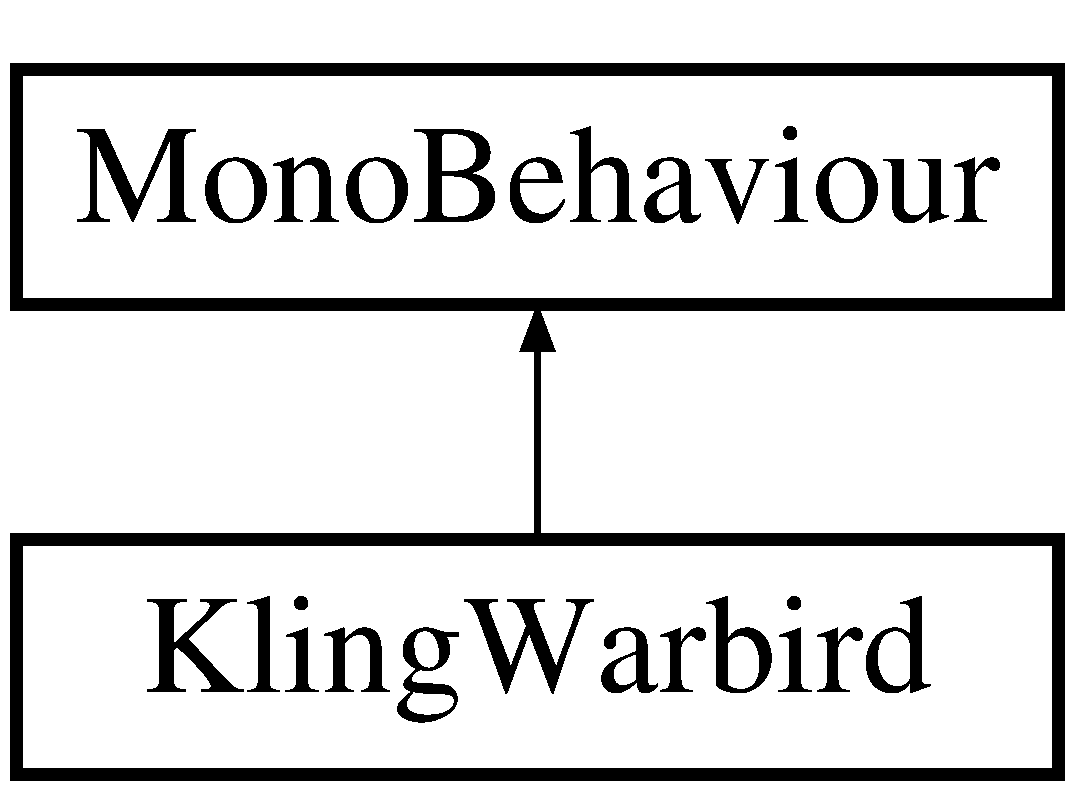
\includegraphics[height=2.000000cm]{class_kling_warbird}
\end{center}
\end{figure}


The documentation for this class was generated from the following file\+:\begin{DoxyCompactItemize}
\item 
/\+Users/\+Leonard/\+Desktop/\+Stor\+Trok/\+Stor Trok/\+Assets/\+Stor Trok/\+Scripts/\+Computer\+Players/\+Spaceships/Kling\+Warbird.\+cs\end{DoxyCompactItemize}

\hypertarget{class_learn_player_movement_data}{}\section{Learn\+Player\+Movement\+Data Class Reference}
\label{class_learn_player_movement_data}\index{Learn\+Player\+Movement\+Data@{Learn\+Player\+Movement\+Data}}
Inheritance diagram for Learn\+Player\+Movement\+Data\+:\begin{figure}[H]
\begin{center}
\leavevmode
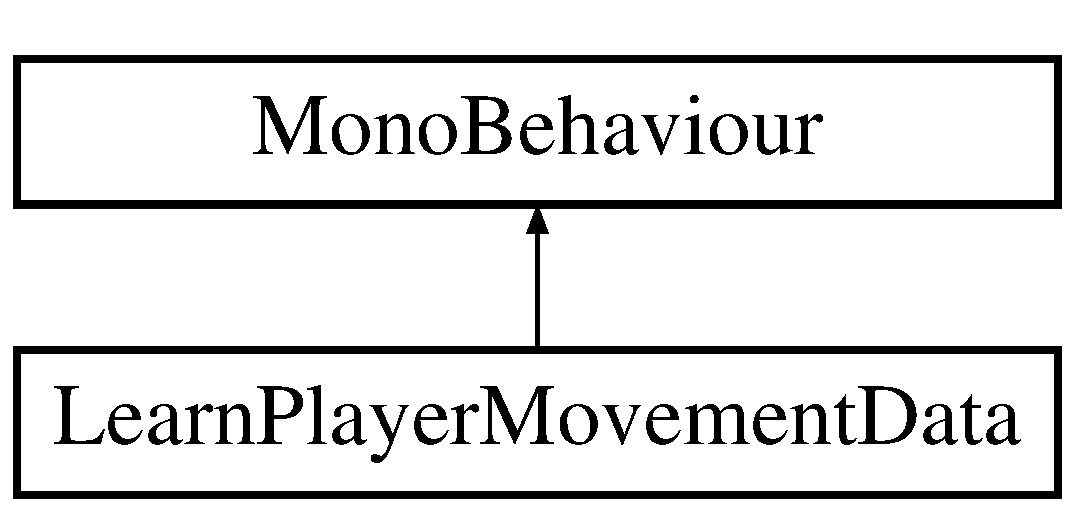
\includegraphics[height=2.000000cm]{class_learn_player_movement_data}
\end{center}
\end{figure}
\subsection*{Public Attributes}
\begin{DoxyCompactItemize}
\item 
\mbox{\Hypertarget{class_learn_player_movement_data_a54c0297008dc7664bc24ea1135d08354}\label{class_learn_player_movement_data_a54c0297008dc7664bc24ea1135d08354}} 
float {\bfseries datapoint\+\_\+learn\+\_\+dtime} = 1
\item 
\mbox{\Hypertarget{class_learn_player_movement_data_aad7ad01cf53e8eb90562a82f4aeb771e}\label{class_learn_player_movement_data_aad7ad01cf53e8eb90562a82f4aeb771e}} 
Game\+Object {\bfseries learn\+\_\+object}
\end{DoxyCompactItemize}


The documentation for this class was generated from the following file\+:\begin{DoxyCompactItemize}
\item 
/\+Users/\+Leonard/\+Desktop/\+Stor\+Trok/\+Stor Trok/\+Assets/\+Stor Trok/\+Scripts/\+Computer\+Players/\+Movement\+Types/\+Movement\+With\+Player\+Data/Learn\+Player\+Movement\+Data.\+cs\end{DoxyCompactItemize}

\hypertarget{class_level_manager}{}\section{Level\+Manager Class Reference}
\label{class_level_manager}\index{Level\+Manager@{Level\+Manager}}
Inheritance diagram for Level\+Manager\+:\begin{figure}[H]
\begin{center}
\leavevmode
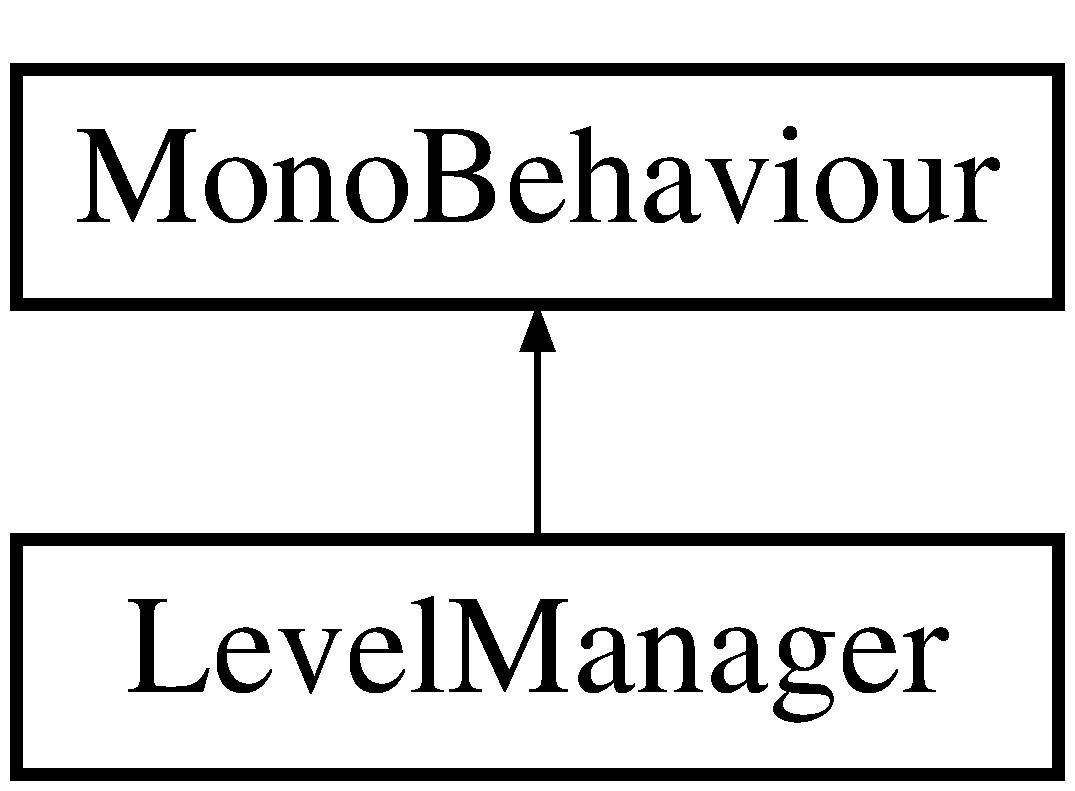
\includegraphics[height=2.000000cm]{class_level_manager}
\end{center}
\end{figure}
\subsection*{Public Member Functions}
\begin{DoxyCompactItemize}
\item 
\mbox{\Hypertarget{class_level_manager_aac4cfd0fe031319eda2f13c30d11414f}\label{class_level_manager_aac4cfd0fe031319eda2f13c30d11414f}} 
void {\bfseries create\+\_\+player\+\_\+space} ()
\item 
\mbox{\Hypertarget{class_level_manager_a553e0f113b0d7cf2cd66a87073ee179e}\label{class_level_manager_a553e0f113b0d7cf2cd66a87073ee179e}} 
void {\bfseries create\+\_\+player\+\_\+ground} ()
\item 
\mbox{\Hypertarget{class_level_manager_a2ec5f6c40499a639a84a4ba8718260c4}\label{class_level_manager_a2ec5f6c40499a639a84a4ba8718260c4}} 
void {\bfseries spawn\+\_\+spaceship} ()
\item 
\mbox{\Hypertarget{class_level_manager_a425d8e50c86371147f0ea622b9f8e639}\label{class_level_manager_a425d8e50c86371147f0ea622b9f8e639}} 
void {\bfseries load\+\_\+new\+\_\+scene} (string scene\+\_\+name)
\item 
\mbox{\Hypertarget{class_level_manager_a3f4447f412ff6d3080246df5d0ea227d}\label{class_level_manager_a3f4447f412ff6d3080246df5d0ea227d}} 
void {\bfseries set\+\_\+pause\+\_\+state} (bool state)
\end{DoxyCompactItemize}
\subsection*{Static Public Member Functions}
\begin{DoxyCompactItemize}
\item 
\mbox{\Hypertarget{class_level_manager_a0a7875c9aa97c40162ac48bf95e9454d}\label{class_level_manager_a0a7875c9aa97c40162ac48bf95e9454d}} 
static void {\bfseries load\+\_\+player\+\_\+data} ()
\item 
\mbox{\Hypertarget{class_level_manager_a6f4409d829188d187674d30bf5832028}\label{class_level_manager_a6f4409d829188d187674d30bf5832028}} 
static void {\bfseries save\+\_\+player\+\_\+data} (bool set\+\_\+ids)
\item 
\mbox{\Hypertarget{class_level_manager_a978a6920356cfd8941a38abcf0133897}\label{class_level_manager_a978a6920356cfd8941a38abcf0133897}} 
static void {\bfseries save\+\_\+player\+\_\+data} ()
\end{DoxyCompactItemize}
\subsection*{Public Attributes}
\begin{DoxyCompactItemize}
\item 
\mbox{\Hypertarget{class_level_manager_afff88b55c30397a71549aa7b26274da3}\label{class_level_manager_afff88b55c30397a71549aa7b26274da3}} 
bool {\bfseries level\+\_\+has\+\_\+mission}
\item 
\mbox{\Hypertarget{class_level_manager_a76878d38e02c611f287dd6b4ad12d294}\label{class_level_manager_a76878d38e02c611f287dd6b4ad12d294}} 
string {\bfseries scene\+\_\+name}
\item 
\mbox{\Hypertarget{class_level_manager_a55c538ae043aef813226b712f8b606e2}\label{class_level_manager_a55c538ae043aef813226b712f8b606e2}} 
readonly float {\bfseries sektorenraum\+\_\+scale\+\_\+factor} = 0.\+04f
\item 
\mbox{\Hypertarget{class_level_manager_a957888d8fbcf2f0e06eed58a6de2f923}\label{class_level_manager_a957888d8fbcf2f0e06eed58a6de2f923}} 
Image {\bfseries fade\+\_\+scene\+\_\+image}
\item 
\mbox{\Hypertarget{class_level_manager_ab27e2c9177cb2ca240756088496d1a52}\label{class_level_manager_ab27e2c9177cb2ca240756088496d1a52}} 
Game\+Object {\bfseries ui}
\item 
\mbox{\Hypertarget{class_level_manager_a96cc13044461a28fe3a30355756c60ef}\label{class_level_manager_a96cc13044461a28fe3a30355756c60ef}} 
Game\+Object {\bfseries spawn\+\_\+point}
\item 
\mbox{\Hypertarget{class_level_manager_a962531eda35efd57cebc72b82eb78566}\label{class_level_manager_a962531eda35efd57cebc72b82eb78566}} 
Transform {\bfseries spaceship\+\_\+spawn\+\_\+point}
\item 
\mbox{\Hypertarget{class_level_manager_abd974d1b5d326ccd9909b487efecc306}\label{class_level_manager_abd974d1b5d326ccd9909b487efecc306}} 
Game\+Object {\bfseries ground\+\_\+player\+\_\+object}
\item 
\mbox{\Hypertarget{class_level_manager_a883489c9372d53358d5db03fbb8ae0f4}\label{class_level_manager_a883489c9372d53358d5db03fbb8ae0f4}} 
bool {\bfseries game\+\_\+paused} = false
\item 
\mbox{\Hypertarget{class_level_manager_a220118be37c8eb414092b279615602b9}\label{class_level_manager_a220118be37c8eb414092b279615602b9}} 
Game\+Object {\bfseries raumschiff\+\_\+object}
\item 
\mbox{\Hypertarget{class_level_manager_ad64a5847ac3d6a167891ce2644cd6628}\label{class_level_manager_ad64a5847ac3d6a167891ce2644cd6628}} 
Game\+Object {\bfseries player\+\_\+game\+Object}
\end{DoxyCompactItemize}
\subsection*{Static Public Attributes}
\begin{DoxyCompactItemize}
\item 
\mbox{\Hypertarget{class_level_manager_ad93295bba6b276adfbca309f9ba36c71}\label{class_level_manager_ad93295bba6b276adfbca309f9ba36c71}} 
static \hyperlink{class_player_data}{Player\+Data} {\bfseries player\+\_\+data}
\item 
\mbox{\Hypertarget{class_level_manager_a0bf70c0b09f89b936ad4646a0985d8b9}\label{class_level_manager_a0bf70c0b09f89b936ad4646a0985d8b9}} 
static \hyperlink{class_level_manager}{Level\+Manager} {\bfseries level\+Manager}
\end{DoxyCompactItemize}


The documentation for this class was generated from the following file\+:\begin{DoxyCompactItemize}
\item 
/\+Users/\+Leonard/\+Desktop/\+Stor\+Trok/\+Stor Trok/\+Assets/\+Stor Trok/\+Scripts/\+Scene\+Masters/Level\+Manager.\+cs\end{DoxyCompactItemize}

\hypertarget{class_minimap}{}\section{Minimap Class Reference}
\label{class_minimap}\index{Minimap@{Minimap}}
Inheritance diagram for Minimap\+:\begin{figure}[H]
\begin{center}
\leavevmode
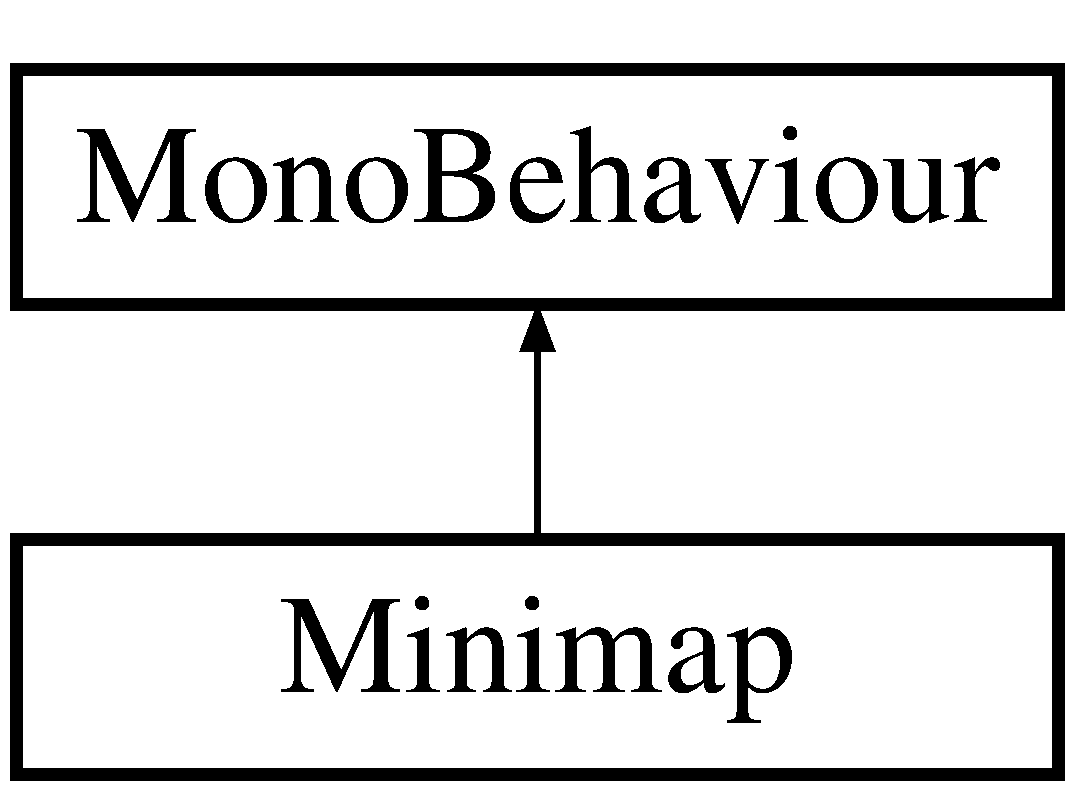
\includegraphics[height=2.000000cm]{class_minimap}
\end{center}
\end{figure}
\subsection*{Public Member Functions}
\begin{DoxyCompactItemize}
\item 
\mbox{\Hypertarget{class_minimap_a299c4a3912d915a76a0681592172c2af}\label{class_minimap_a299c4a3912d915a76a0681592172c2af}} 
void {\bfseries check\+\_\+objects} ()
\end{DoxyCompactItemize}
\subsection*{Public Attributes}
\begin{DoxyCompactItemize}
\item 
\mbox{\Hypertarget{class_minimap_a36deafcdb203f234551ed1fe2bb9f557}\label{class_minimap_a36deafcdb203f234551ed1fe2bb9f557}} 
Texture {\bfseries enemy}
\item 
\mbox{\Hypertarget{class_minimap_a3586ee859abcf78c3929bfe474224d95}\label{class_minimap_a3586ee859abcf78c3929bfe474224d95}} 
Texture {\bfseries player}
\item 
\mbox{\Hypertarget{class_minimap_a8a72cb7101c9ae06543511f9269d0b54}\label{class_minimap_a8a72cb7101c9ae06543511f9269d0b54}} 
Texture {\bfseries ally}
\item 
\mbox{\Hypertarget{class_minimap_a8bcb3dee58defac9a40b22cd4234b7ab}\label{class_minimap_a8bcb3dee58defac9a40b22cd4234b7ab}} 
Game\+Object {\bfseries minimap\+\_\+object}
\item 
\mbox{\Hypertarget{class_minimap_a7b9a24c2f296ac38de11c72fc5460e05}\label{class_minimap_a7b9a24c2f296ac38de11c72fc5460e05}} 
const float {\bfseries minimap\+\_\+object\+\_\+size} = 20
\item 
\mbox{\Hypertarget{class_minimap_a7eaf8d1c5242b1e38394344edf0d5af8}\label{class_minimap_a7eaf8d1c5242b1e38394344edf0d5af8}} 
Line\+Renderer {\bfseries player\+\_\+attack\+\_\+range}
\item 
\mbox{\Hypertarget{class_minimap_aa0741c6e8c34b3a9eb0268aa412f16d4}\label{class_minimap_aa0741c6e8c34b3a9eb0268aa412f16d4}} 
const int {\bfseries number\+\_\+of\+\_\+attack\+\_\+range\+\_\+points} = 40
\item 
\mbox{\Hypertarget{class_minimap_ac35ee8e69cf5e93c504aefaf0b2b6d0d}\label{class_minimap_ac35ee8e69cf5e93c504aefaf0b2b6d0d}} 
Transform {\bfseries minimap\+\_\+camera}
\item 
\mbox{\Hypertarget{class_minimap_a0a2c7f72de980c606ce16cc03e9bdf17}\label{class_minimap_a0a2c7f72de980c606ce16cc03e9bdf17}} 
Transform {\bfseries minimap\+\_\+camera\+\_\+range}
\item 
\mbox{\Hypertarget{class_minimap_a34ceb23acba0adfc0939139a171032cd}\label{class_minimap_a34ceb23acba0adfc0939139a171032cd}} 
const float {\bfseries camera\+\_\+range\+\_\+length} = 1000
\end{DoxyCompactItemize}
\subsection*{Properties}
\begin{DoxyCompactItemize}
\item 
\mbox{\Hypertarget{class_minimap_acf0ff370a30f4c5a55a424fb18b91483}\label{class_minimap_acf0ff370a30f4c5a55a424fb18b91483}} 
static \hyperlink{class_minimap}{Minimap} {\bfseries minimap}\hspace{0.3cm}{\ttfamily  \mbox{[}get, set\mbox{]}}
\end{DoxyCompactItemize}


The documentation for this class was generated from the following file\+:\begin{DoxyCompactItemize}
\item 
/\+Users/\+Leonard/\+Desktop/\+Stor\+Trok/\+Stor Trok/\+Assets/\+Stor Trok/\+Scripts/\+U\+I/\+Minimap/Minimap.\+cs\end{DoxyCompactItemize}

\hypertarget{class_minimap_object}{}\section{Minimap\+Object Class Reference}
\label{class_minimap_object}\index{Minimap\+Object@{Minimap\+Object}}
Inheritance diagram for Minimap\+Object\+:\begin{figure}[H]
\begin{center}
\leavevmode
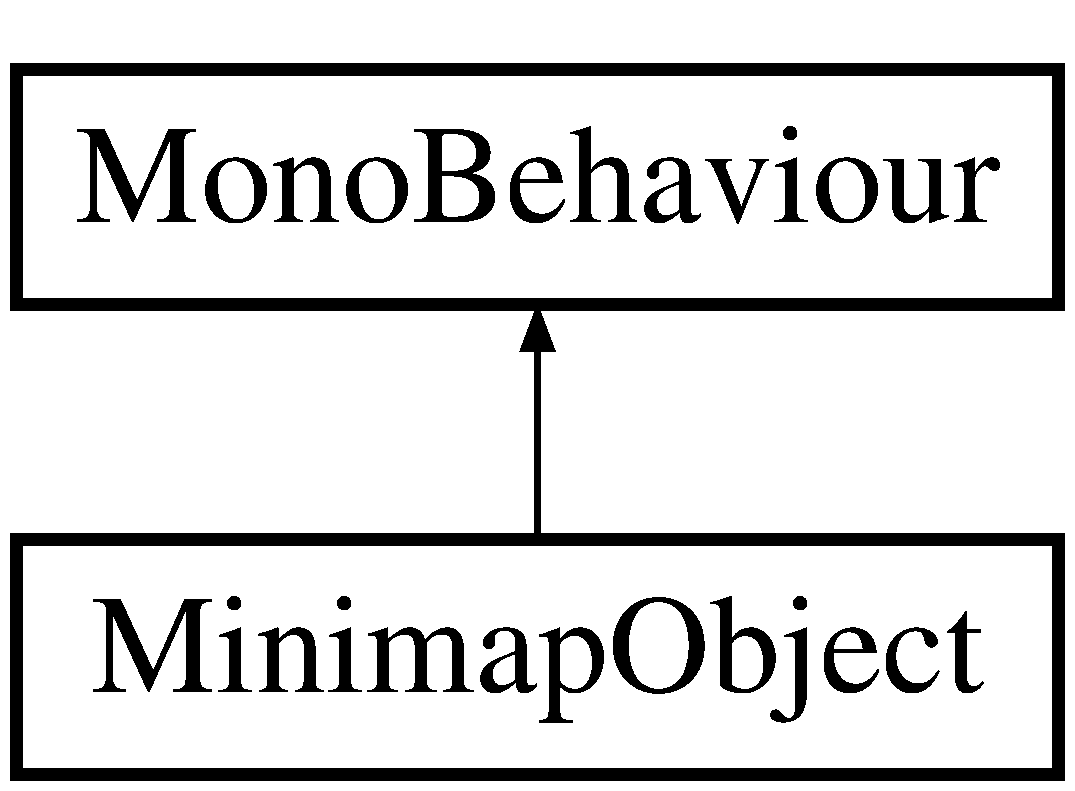
\includegraphics[height=2.000000cm]{class_minimap_object}
\end{center}
\end{figure}
\subsection*{Public Attributes}
\begin{DoxyCompactItemize}
\item 
\mbox{\Hypertarget{class_minimap_object_afa7543be4741d229023738ee5483e74f}\label{class_minimap_object_afa7543be4741d229023738ee5483e74f}} 
Transform {\bfseries object\+\_\+to\+\_\+represent}
\item 
\mbox{\Hypertarget{class_minimap_object_a95b0ed31b33212c4a618f9b029327b65}\label{class_minimap_object_a95b0ed31b33212c4a618f9b029327b65}} 
bool {\bfseries use\+\_\+minimap\+\_\+object\+\_\+size} = true
\end{DoxyCompactItemize}
\subsection*{Static Public Attributes}
\begin{DoxyCompactItemize}
\item 
\mbox{\Hypertarget{class_minimap_object_afae247d677a3f7fa91d5e145e7ff4cbd}\label{class_minimap_object_afae247d677a3f7fa91d5e145e7ff4cbd}} 
static List$<$ \hyperlink{class_minimap_object}{Minimap\+Object} $>$ {\bfseries all\+\_\+minimap\+\_\+objects} = new List$<$\hyperlink{class_minimap_object}{Minimap\+Object}$>$()
\end{DoxyCompactItemize}


The documentation for this class was generated from the following file\+:\begin{DoxyCompactItemize}
\item 
/\+Users/\+Leonard/\+Desktop/\+Stor\+Trok/\+Stor Trok/\+Assets/\+Stor Trok/\+Scripts/\+U\+I/\+Minimap/Minimap\+Object.\+cs\end{DoxyCompactItemize}

\hypertarget{class_mission}{}\section{Mission Class Reference}
\label{class_mission}\index{Mission@{Mission}}
Inheritance diagram for Mission\+:\begin{figure}[H]
\begin{center}
\leavevmode
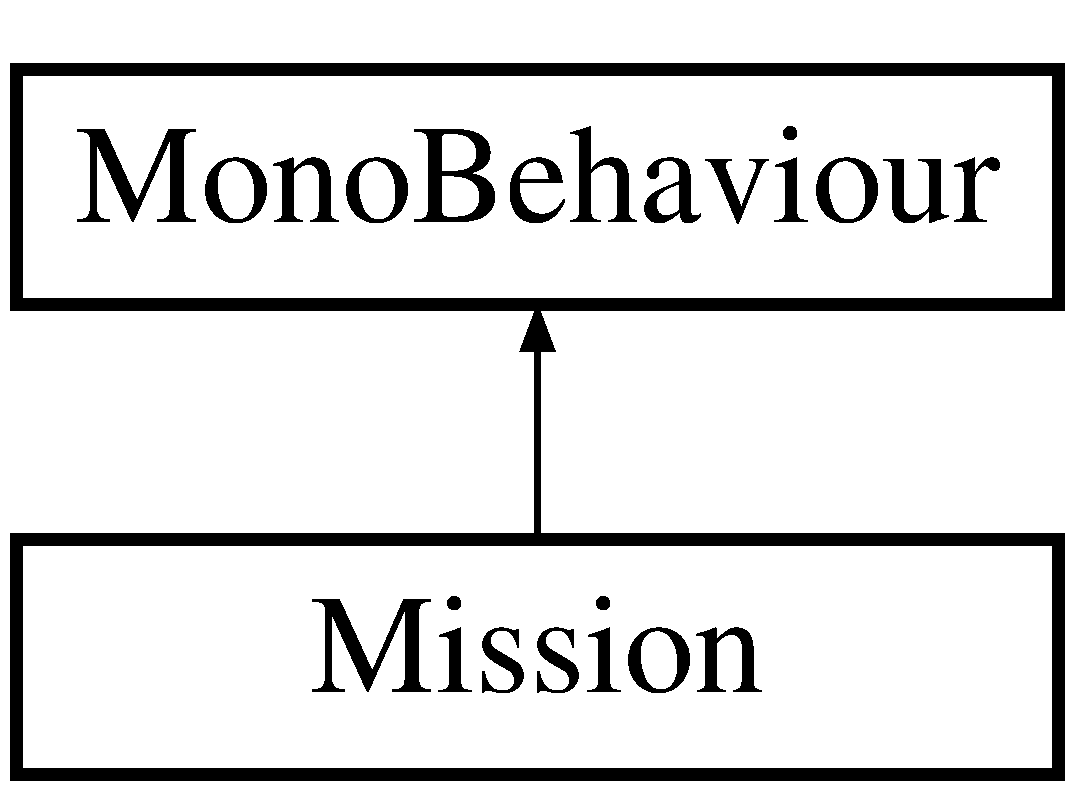
\includegraphics[height=2.000000cm]{class_mission}
\end{center}
\end{figure}
\subsection*{Public Member Functions}
\begin{DoxyCompactItemize}
\item 
\mbox{\Hypertarget{class_mission_ad59e9b9c65b611f73b36f6f637c69f4c}\label{class_mission_ad59e9b9c65b611f73b36f6f637c69f4c}} 
void {\bfseries disable\+\_\+all\+\_\+enemies} ()
\item 
\mbox{\Hypertarget{class_mission_ae952b8f9de6ba1cf5a4b6b7545b007e1}\label{class_mission_ae952b8f9de6ba1cf5a4b6b7545b007e1}} 
void {\bfseries load\+\_\+new\+\_\+mission\+\_\+part} (\hyperlink{class_mission_part}{Mission\+Part} m, bool keep\+\_\+destroyed\+\_\+spaceships)
\item 
\mbox{\Hypertarget{class_mission_a17df837067548e1008b0e61da6ea1c30}\label{class_mission_a17df837067548e1008b0e61da6ea1c30}} 
void {\bfseries start\+\_\+change\+\_\+camera\+\_\+focus} ()
\item 
\mbox{\Hypertarget{class_mission_a78d4acd4bb6740d22eafdc3339926a0e}\label{class_mission_a78d4acd4bb6740d22eafdc3339926a0e}} 
void {\bfseries check\+\_\+status} ()
\item 
\mbox{\Hypertarget{class_mission_a446a3df52e395307c2835f39672f4b19}\label{class_mission_a446a3df52e395307c2835f39672f4b19}} 
void {\bfseries quit\+\_\+mission} ()
\item 
\mbox{\Hypertarget{class_mission_a465f5f4e76c4626e2044d7680ed64faf}\label{class_mission_a465f5f4e76c4626e2044d7680ed64faf}} 
void {\bfseries start\+\_\+mission} ()
\end{DoxyCompactItemize}
\subsection*{Public Attributes}
\begin{DoxyCompactItemize}
\item 
\mbox{\Hypertarget{class_mission_a3272ee986e1263d7e84667e4da3efef6}\label{class_mission_a3272ee986e1263d7e84667e4da3efef6}} 
Player\+Environment\+Status {\bfseries environment\+\_\+type}
\item 
\mbox{\Hypertarget{class_mission_a8af9bf41bf75c2e6c2371ae648ec8508}\label{class_mission_a8af9bf41bf75c2e6c2371ae648ec8508}} 
\hyperlink{class_full_mission}{Full\+Mission} {\bfseries full\+Mission}
\item 
\mbox{\Hypertarget{class_mission_a7cfb32ad3e950150fc5cd542111fb1cf}\label{class_mission_a7cfb32ad3e950150fc5cd542111fb1cf}} 
Game\+Object {\bfseries camera\+\_\+start\+\_\+point}
\item 
\mbox{\Hypertarget{class_mission_acd86a0869fb24b9535104f7eb21e7332}\label{class_mission_acd86a0869fb24b9535104f7eb21e7332}} 
Mission\+Status {\bfseries mission\+\_\+status}
\end{DoxyCompactItemize}
\subsection*{Static Public Attributes}
\begin{DoxyCompactItemize}
\item 
\mbox{\Hypertarget{class_mission_aa537dedc4dcd1d7ae6662ecf614bbea1}\label{class_mission_aa537dedc4dcd1d7ae6662ecf614bbea1}} 
static \hyperlink{class_mission}{Mission} {\bfseries current\+\_\+mission}
\end{DoxyCompactItemize}


The documentation for this class was generated from the following file\+:\begin{DoxyCompactItemize}
\item 
/\+Users/\+Leonard/\+Desktop/\+Stor\+Trok/\+Stor Trok/\+Assets/\+Stor Trok/\+Scripts/\+Mission/Mission.\+cs\end{DoxyCompactItemize}

\hypertarget{class_mission_data}{}\section{Mission\+Data Class Reference}
\label{class_mission_data}\index{Mission\+Data@{Mission\+Data}}
Inheritance diagram for Mission\+Data\+:\begin{figure}[H]
\begin{center}
\leavevmode
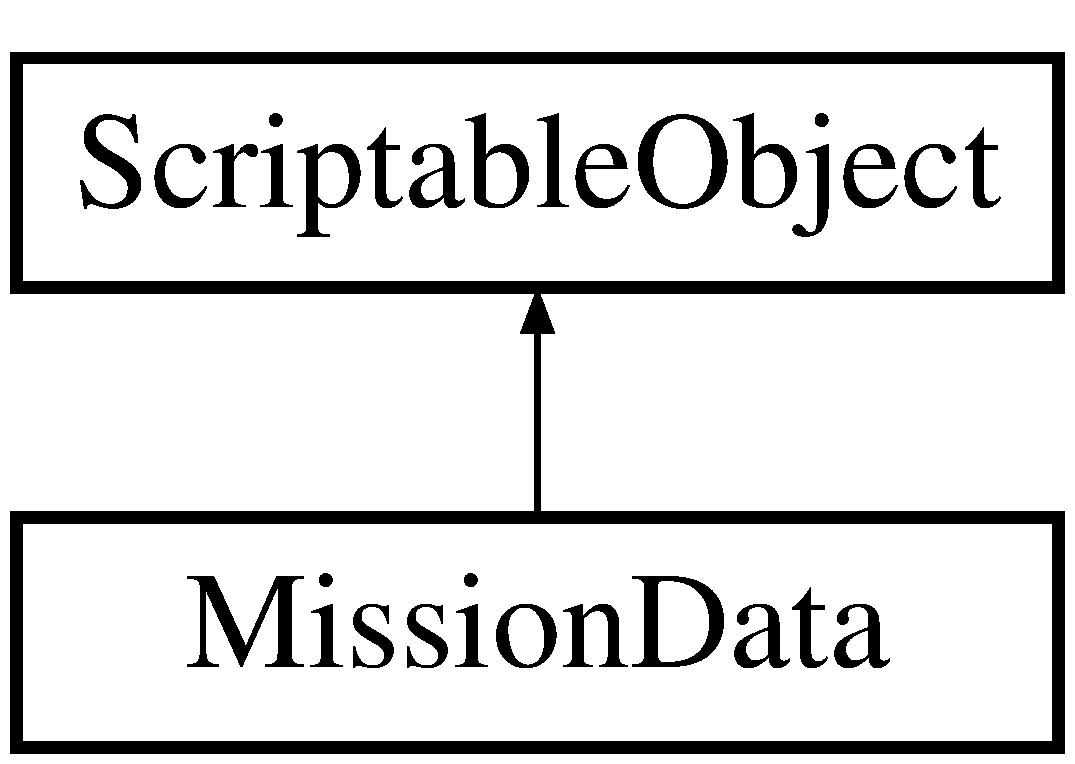
\includegraphics[height=2.000000cm]{class_mission_data}
\end{center}
\end{figure}
\subsection*{Public Attributes}
\begin{DoxyCompactItemize}
\item 
\mbox{\Hypertarget{class_mission_data_a6afc5ff5ddb309b831a55f12b48027ab}\label{class_mission_data_a6afc5ff5ddb309b831a55f12b48027ab}} 
int {\bfseries ID}
\item 
\mbox{\Hypertarget{class_mission_data_ab48eb25317f3d91e77d46f15721b90f8}\label{class_mission_data_ab48eb25317f3d91e77d46f15721b90f8}} 
int {\bfseries planet\+\_\+system\+\_\+\+ID}
\item 
\mbox{\Hypertarget{class_mission_data_add60fd614e36666f17fc74e102fd99bd}\label{class_mission_data_add60fd614e36666f17fc74e102fd99bd}} 
string {\bfseries scene\+\_\+name}
\item 
\mbox{\Hypertarget{class_mission_data_ab33174ebf8bed859623c5ec422691808}\label{class_mission_data_ab33174ebf8bed859623c5ec422691808}} 
string {\bfseries title}
\item 
\mbox{\Hypertarget{class_mission_data_ae30ca292edaa7d3e09ec8beee9b0b214}\label{class_mission_data_ae30ca292edaa7d3e09ec8beee9b0b214}} 
string {\bfseries description}
\end{DoxyCompactItemize}
\subsection*{Static Public Attributes}
\begin{DoxyCompactItemize}
\item 
\mbox{\Hypertarget{class_mission_data_a0b2830f0d97e90ef5fa1362128e0e16b}\label{class_mission_data_a0b2830f0d97e90ef5fa1362128e0e16b}} 
static List$<$ \hyperlink{class_mission_data}{Mission\+Data} $>$ {\bfseries all\+\_\+misson\+\_\+datas} = new List$<$\hyperlink{class_mission_data}{Mission\+Data}$>$()
\end{DoxyCompactItemize}


The documentation for this class was generated from the following file\+:\begin{DoxyCompactItemize}
\item 
/\+Users/\+Leonard/\+Desktop/\+Stor\+Trok/\+Stor Trok/\+Assets/\+Stor Trok/\+Scripts/\+Planet\+System/Mission\+Data.\+cs\end{DoxyCompactItemize}

\hypertarget{class_mission_enemy}{}\section{Mission\+Enemy Class Reference}
\label{class_mission_enemy}\index{Mission\+Enemy@{Mission\+Enemy}}
\subsection*{Public Attributes}
\begin{DoxyCompactItemize}
\item 
\mbox{\Hypertarget{class_mission_enemy_a00c8cfc36791fc0c7408fa3075780f95}\label{class_mission_enemy_a00c8cfc36791fc0c7408fa3075780f95}} 
\hyperlink{class_spaceship}{Spaceship} {\bfseries enemy}
\item 
\mbox{\Hypertarget{class_mission_enemy_ab8c8ef90135f0490d8ffc1b33b721a29}\label{class_mission_enemy_ab8c8ef90135f0490d8ffc1b33b721a29}} 
bool {\bfseries warps\+\_\+in\+\_\+at\+\_\+missionpart\+\_\+start}
\end{DoxyCompactItemize}


The documentation for this class was generated from the following file\+:\begin{DoxyCompactItemize}
\item 
/\+Users/\+Leonard/\+Desktop/\+Stor\+Trok/\+Stor Trok/\+Assets/\+Stor Trok/\+Scripts/\+Mission/Mission\+Part.\+cs\end{DoxyCompactItemize}

\hypertarget{class_mission_goal}{}\section{Mission\+Goal Class Reference}
\label{class_mission_goal}\index{Mission\+Goal@{Mission\+Goal}}
\subsection*{Public Attributes}
\begin{DoxyCompactItemize}
\item 
\mbox{\Hypertarget{class_mission_goal_a9966e7c7f87310cf5ee05d1b82c14d58}\label{class_mission_goal_a9966e7c7f87310cf5ee05d1b82c14d58}} 
Game\+Object {\bfseries target}
\item 
\mbox{\Hypertarget{class_mission_goal_af6c0889b1323e84b5d807b7cac66dae6}\label{class_mission_goal_af6c0889b1323e84b5d807b7cac66dae6}} 
Mission\+Goal\+Types {\bfseries mission\+\_\+goal\+\_\+type}
\item 
\mbox{\Hypertarget{class_mission_goal_a98bf20ed825965d862be7e4b483f088f}\label{class_mission_goal_a98bf20ed825965d862be7e4b483f088f}} 
bool {\bfseries warps\+\_\+in\+\_\+at\+\_\+missionpart\+\_\+start}
\item 
\mbox{\Hypertarget{class_mission_goal_a0aa2cc35db69de3bf290e8a63d457f86}\label{class_mission_goal_a0aa2cc35db69de3bf290e8a63d457f86}} 
bool {\bfseries focus\+\_\+camera\+\_\+on\+\_\+object\+\_\+at\+\_\+missionpart\+\_\+start}
\item 
\mbox{\Hypertarget{class_mission_goal_a8a46e7994b5b75ebb35b67ec459f6344}\label{class_mission_goal_a8a46e7994b5b75ebb35b67ec459f6344}} 
bool {\bfseries goal\+\_\+achieved} = false
\end{DoxyCompactItemize}


The documentation for this class was generated from the following file\+:\begin{DoxyCompactItemize}
\item 
/\+Users/\+Leonard/\+Desktop/\+Stor\+Trok/\+Stor Trok/\+Assets/\+Stor Trok/\+Scripts/\+Mission/Mission\+Part.\+cs\end{DoxyCompactItemize}

\hypertarget{class_mission_part}{}\section{Mission\+Part Class Reference}
\label{class_mission_part}\index{Mission\+Part@{Mission\+Part}}
\subsection*{Public Attributes}
\begin{DoxyCompactItemize}
\item 
\mbox{\Hypertarget{class_mission_part_a7e3b429a941f86f1ee3ea2744413c097}\label{class_mission_part_a7e3b429a941f86f1ee3ea2744413c097}} 
int {\bfseries ID}
\item 
\mbox{\Hypertarget{class_mission_part_a815fed1039a22528fa2e67349a9e7e84}\label{class_mission_part_a815fed1039a22528fa2e67349a9e7e84}} 
string {\bfseries title}
\item 
\mbox{\Hypertarget{class_mission_part_a1f79bfaa4907bb57f8d92318953f0cac}\label{class_mission_part_a1f79bfaa4907bb57f8d92318953f0cac}} 
string {\bfseries description}
\item 
\mbox{\Hypertarget{class_mission_part_ac0d1ca7919c1752e38c464cc2d7545a6}\label{class_mission_part_ac0d1ca7919c1752e38c464cc2d7545a6}} 
List$<$ \hyperlink{class_mission_goal}{Mission\+Goal} $>$ {\bfseries mission\+\_\+goals}
\end{DoxyCompactItemize}


The documentation for this class was generated from the following file\+:\begin{DoxyCompactItemize}
\item 
/\+Users/\+Leonard/\+Desktop/\+Stor\+Trok/\+Stor Trok/\+Assets/\+Stor Trok/\+Scripts/\+Mission/Mission\+Part.\+cs\end{DoxyCompactItemize}

\hypertarget{class_navigation_path}{}\section{Navigation\+Path Class Reference}
\label{class_navigation_path}\index{Navigation\+Path@{Navigation\+Path}}
\subsection*{Public Attributes}
\begin{DoxyCompactItemize}
\item 
\mbox{\Hypertarget{class_navigation_path_a41bd7f90ea533bd623047d68678670cf}\label{class_navigation_path_a41bd7f90ea533bd623047d68678670cf}} 
bool {\bfseries looping}
\item 
\mbox{\Hypertarget{class_navigation_path_a25585b1b1e8d0e88fed5520f9af16211}\label{class_navigation_path_a25585b1b1e8d0e88fed5520f9af16211}} 
float {\bfseries target\+\_\+speed}
\item 
\mbox{\Hypertarget{class_navigation_path_a657e5ffa623f45127b5358acba7a92a4}\label{class_navigation_path_a657e5ffa623f45127b5358acba7a92a4}} 
Transform \mbox{[}$\,$\mbox{]} {\bfseries waypoints}
\item 
\mbox{\Hypertarget{class_navigation_path_a296755ab47dac794e7cf1e49437bfa96}\label{class_navigation_path_a296755ab47dac794e7cf1e49437bfa96}} 
int {\bfseries current\+\_\+target\+\_\+waypoint} = 0
\end{DoxyCompactItemize}


The documentation for this class was generated from the following file\+:\begin{DoxyCompactItemize}
\item 
/\+Users/\+Leonard/\+Desktop/\+Stor\+Trok/\+Stor Trok/\+Assets/\+Stor Trok/\+Scripts/Navigation\+Path.\+cs\end{DoxyCompactItemize}

\hypertarget{class_navigation_path_movement}{}\section{Navigation\+Path\+Movement Class Reference}
\label{class_navigation_path_movement}\index{Navigation\+Path\+Movement@{Navigation\+Path\+Movement}}
Inheritance diagram for Navigation\+Path\+Movement\+:\begin{figure}[H]
\begin{center}
\leavevmode
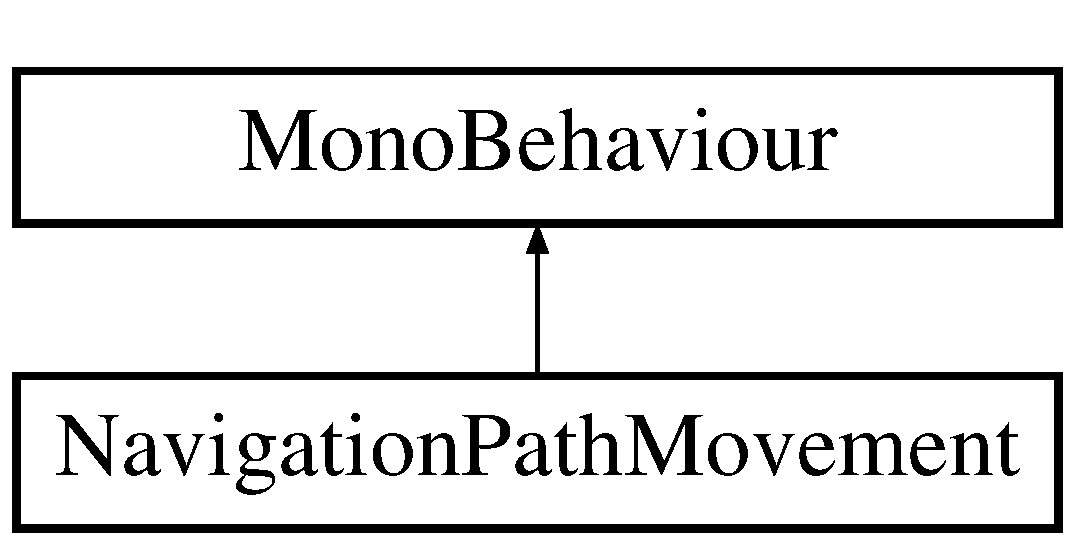
\includegraphics[height=2.000000cm]{class_navigation_path_movement}
\end{center}
\end{figure}
\subsection*{Public Attributes}
\begin{DoxyCompactItemize}
\item 
\mbox{\Hypertarget{class_navigation_path_movement_a9f4a2b40391b762dcf690694ed9f16b9}\label{class_navigation_path_movement_a9f4a2b40391b762dcf690694ed9f16b9}} 
\hyperlink{class_navigation_path}{Navigation\+Path} {\bfseries navigation\+\_\+path}
\item 
\mbox{\Hypertarget{class_navigation_path_movement_a692e7ad3c064c9e97a0d5db065aed3f0}\label{class_navigation_path_movement_a692e7ad3c064c9e97a0d5db065aed3f0}} 
bool {\bfseries finished\+\_\+following\+\_\+path} = false
\end{DoxyCompactItemize}


The documentation for this class was generated from the following file\+:\begin{DoxyCompactItemize}
\item 
/\+Users/\+Leonard/\+Desktop/\+Stor\+Trok/\+Stor Trok/\+Assets/\+Stor Trok/\+Scripts/\+Computer\+Players/\+Movement\+Types/Navigation\+Path\+Movement.\+cs\end{DoxyCompactItemize}

\hypertarget{class_nebula}{}\section{Nebula Class Reference}
\label{class_nebula}\index{Nebula@{Nebula}}
Inheritance diagram for Nebula\+:\begin{figure}[H]
\begin{center}
\leavevmode
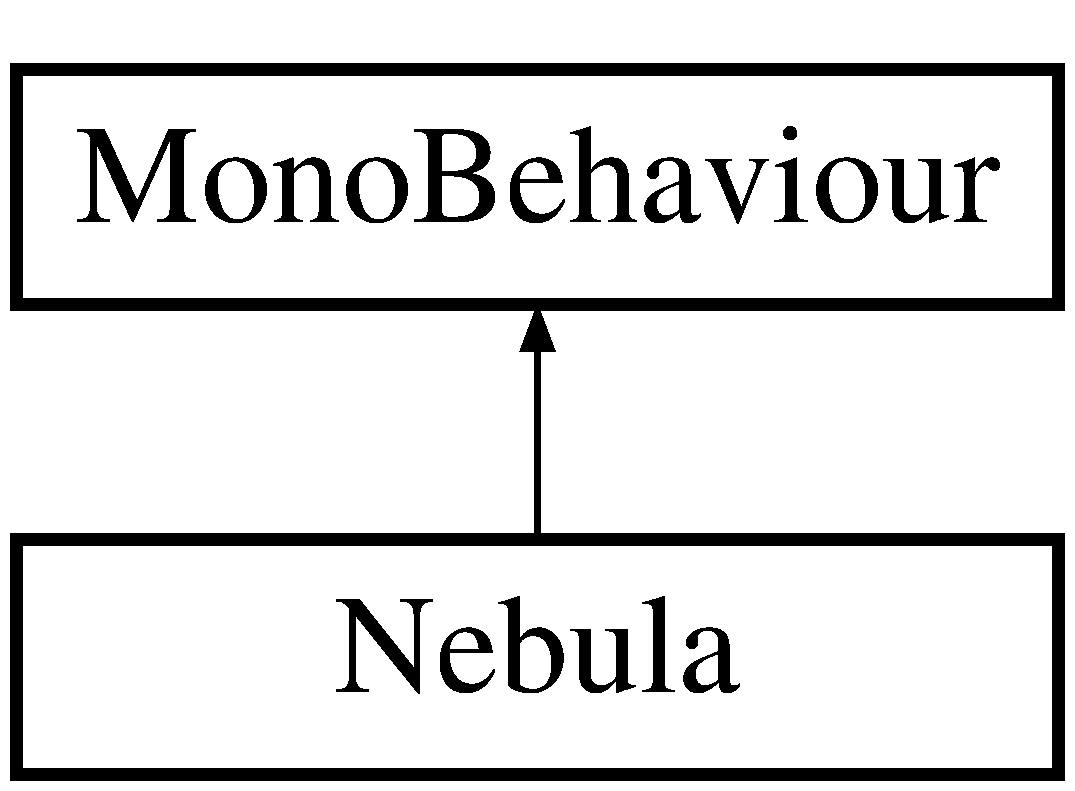
\includegraphics[height=2.000000cm]{class_nebula}
\end{center}
\end{figure}
\subsection*{Public Attributes}
\begin{DoxyCompactItemize}
\item 
\mbox{\Hypertarget{class_nebula_aa9311aa6a4beb53e52c649a286e8ad47}\label{class_nebula_aa9311aa6a4beb53e52c649a286e8ad47}} 
Game\+Object {\bfseries nebula\+\_\+plane}
\item 
\mbox{\Hypertarget{class_nebula_a20a8755c3875c3b075f0ed8d53ca341c}\label{class_nebula_a20a8755c3875c3b075f0ed8d53ca341c}} 
int {\bfseries number\+\_\+of\+\_\+planes} = 20
\end{DoxyCompactItemize}


The documentation for this class was generated from the following file\+:\begin{DoxyCompactItemize}
\item 
/\+Users/\+Leonard/\+Desktop/\+Stor\+Trok/\+Stor Trok/\+Assets/\+Stor Trok/\+Scripts/\+Tests/Nebula.\+cs\end{DoxyCompactItemize}

\hypertarget{class_object_aura}{}\section{Object\+Aura Class Reference}
\label{class_object_aura}\index{Object\+Aura@{Object\+Aura}}
Inheritance diagram for Object\+Aura\+:\begin{figure}[H]
\begin{center}
\leavevmode
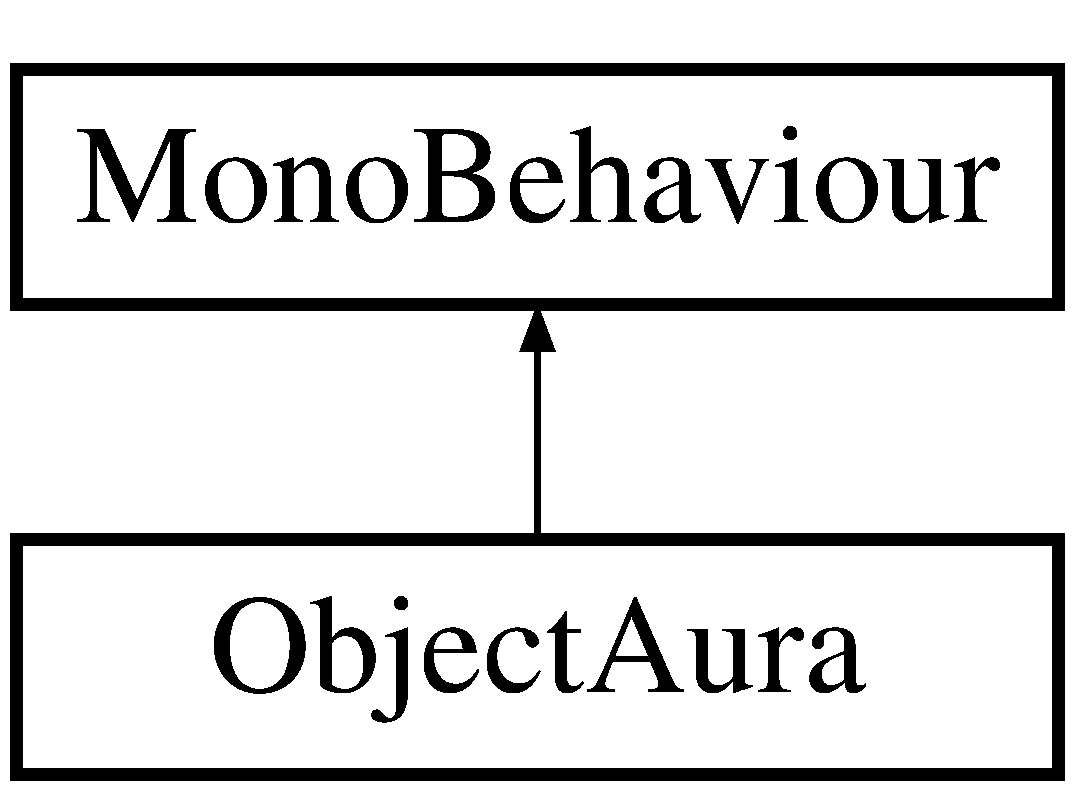
\includegraphics[height=2.000000cm]{class_object_aura}
\end{center}
\end{figure}
\subsection*{Public Attributes}
\begin{DoxyCompactItemize}
\item 
\mbox{\Hypertarget{class_object_aura_a8a40c5c9b02bb48f5934154baf5a8087}\label{class_object_aura_a8a40c5c9b02bb48f5934154baf5a8087}} 
bool {\bfseries player\+\_\+in\+\_\+aura}
\item 
\mbox{\Hypertarget{class_object_aura_a50640a47a2757545614081176cf57816}\label{class_object_aura_a50640a47a2757545614081176cf57816}} 
Object\+Aura\+Type {\bfseries object\+Aura\+Type}
\item 
\mbox{\Hypertarget{class_object_aura_a4b9a0fff7f66a23a37cef92e5bd3db26}\label{class_object_aura_a4b9a0fff7f66a23a37cef92e5bd3db26}} 
bool {\bfseries interactive\+\_\+message\+\_\+generated} = false
\item 
\mbox{\Hypertarget{class_object_aura_a337f83b23b4547f0719d2b3146391a97}\label{class_object_aura_a337f83b23b4547f0719d2b3146391a97}} 
List$<$ \hyperlink{class_interactive_message_button}{Interactive\+Message\+Button} $>$ {\bfseries interactive\+\_\+message\+\_\+buttons} = new List$<$\hyperlink{class_interactive_message_button}{Interactive\+Message\+Button}$>$ ()
\item 
\mbox{\Hypertarget{class_object_aura_a68d5255fca157109649b8b19aeffbd17}\label{class_object_aura_a68d5255fca157109649b8b19aeffbd17}} 
bool {\bfseries check\+\_\+distance} = false
\item 
\mbox{\Hypertarget{class_object_aura_a3b940ca33764a9a82af38b4dff1fe600}\label{class_object_aura_a3b940ca33764a9a82af38b4dff1fe600}} 
float {\bfseries radius}
\end{DoxyCompactItemize}
\subsection*{Static Public Attributes}
\begin{DoxyCompactItemize}
\item 
\mbox{\Hypertarget{class_object_aura_a252f79dcddf2bc70c559f0ca499accb3}\label{class_object_aura_a252f79dcddf2bc70c559f0ca499accb3}} 
static List$<$ \hyperlink{class_object_aura}{Object\+Aura} $>$ {\bfseries object\+Auras\+Player\+Is\+In} = new List$<$\hyperlink{class_object_aura}{Object\+Aura}$>$ ()
\end{DoxyCompactItemize}


The documentation for this class was generated from the following file\+:\begin{DoxyCompactItemize}
\item 
/\+Users/\+Leonard/\+Desktop/\+Stor\+Trok/\+Stor Trok/\+Assets/\+Stor Trok/\+Scripts/Object\+Aura.\+cs\end{DoxyCompactItemize}

\hypertarget{class_other_prefab_objects}{}\section{Other\+Prefab\+Objects Class Reference}
\label{class_other_prefab_objects}\index{Other\+Prefab\+Objects@{Other\+Prefab\+Objects}}
Inheritance diagram for Other\+Prefab\+Objects\+:\begin{figure}[H]
\begin{center}
\leavevmode
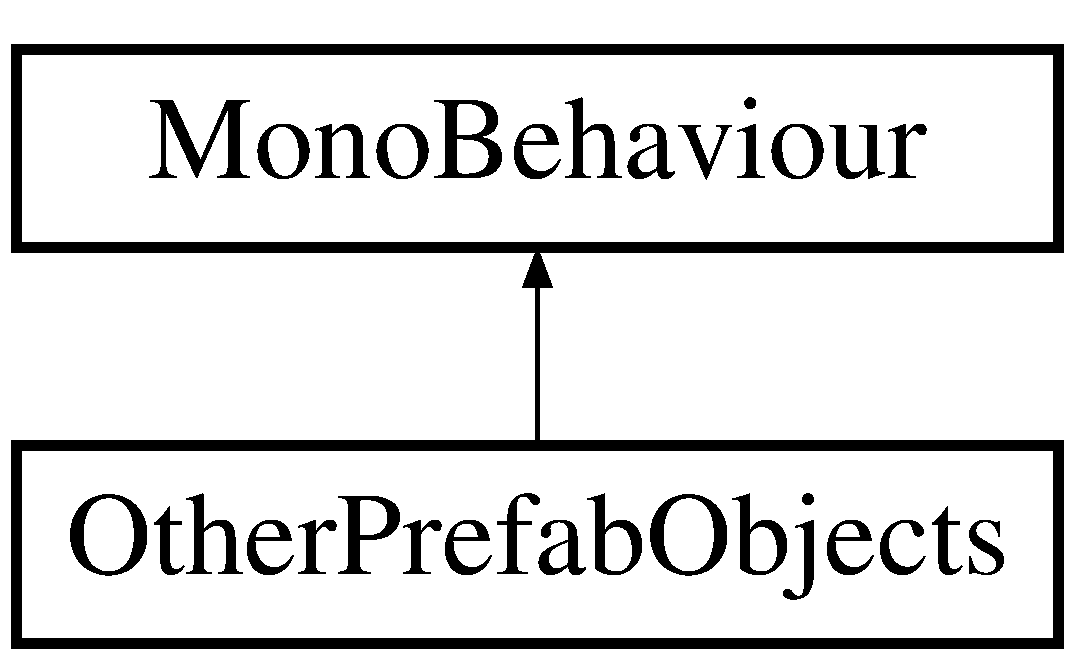
\includegraphics[height=2.000000cm]{class_other_prefab_objects}
\end{center}
\end{figure}
\subsection*{Public Attributes}
\begin{DoxyCompactItemize}
\item 
\mbox{\Hypertarget{class_other_prefab_objects_a9ef93f4ba771a8d4b231425bd9a62cf8}\label{class_other_prefab_objects_a9ef93f4ba771a8d4b231425bd9a62cf8}} 
Game\+Object {\bfseries drop\+\_\+object}
\item 
\mbox{\Hypertarget{class_other_prefab_objects_a8a304d25560256bd1c78268c968b3c88}\label{class_other_prefab_objects_a8a304d25560256bd1c78268c968b3c88}} 
Game\+Object {\bfseries interactive\+\_\+message\+\_\+button}
\item 
\mbox{\Hypertarget{class_other_prefab_objects_a12043ad62ab00a21487a5ab5b270795e}\label{class_other_prefab_objects_a12043ad62ab00a21487a5ab5b270795e}} 
Game\+Object {\bfseries text3D}
\item 
\mbox{\Hypertarget{class_other_prefab_objects_a180d4e030b4bac7db1220dcf227812d4}\label{class_other_prefab_objects_a180d4e030b4bac7db1220dcf227812d4}} 
Game\+Object {\bfseries ship\+\_\+explosion}
\end{DoxyCompactItemize}
\subsection*{Static Public Attributes}
\begin{DoxyCompactItemize}
\item 
\mbox{\Hypertarget{class_other_prefab_objects_aa8c46bf0e16934c4a5d4a9cfc8b57c3f}\label{class_other_prefab_objects_aa8c46bf0e16934c4a5d4a9cfc8b57c3f}} 
static \hyperlink{class_other_prefab_objects}{Other\+Prefab\+Objects} {\bfseries other\+Prefab\+Objects}
\end{DoxyCompactItemize}


The documentation for this class was generated from the following file\+:\begin{DoxyCompactItemize}
\item 
/\+Users/\+Leonard/\+Desktop/\+Stor\+Trok/\+Stor Trok/\+Assets/\+Stor Trok/\+Scripts/\+Asset\+Classes/Other\+Prefab\+Objects.\+cs\end{DoxyCompactItemize}

\hypertarget{class_pause_menu}{}\section{Pause\+Menu Class Reference}
\label{class_pause_menu}\index{Pause\+Menu@{Pause\+Menu}}
Inheritance diagram for Pause\+Menu\+:\begin{figure}[H]
\begin{center}
\leavevmode
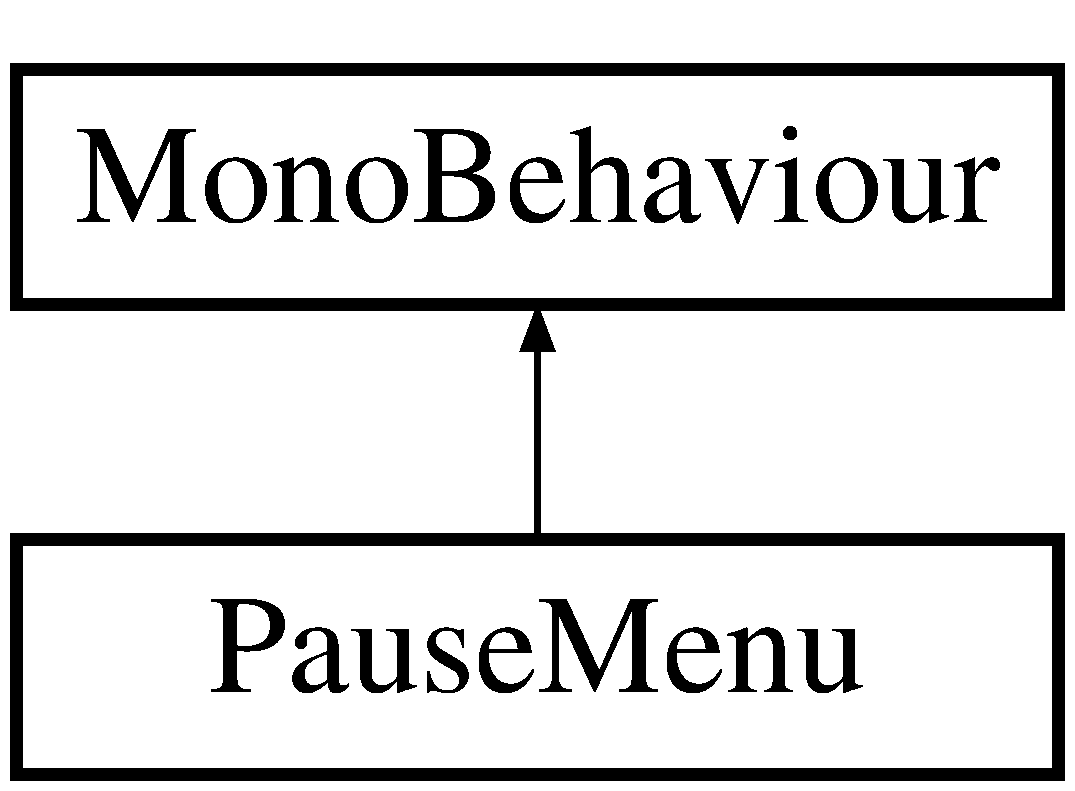
\includegraphics[height=2.000000cm]{class_pause_menu}
\end{center}
\end{figure}
\subsection*{Public Member Functions}
\begin{DoxyCompactItemize}
\item 
\mbox{\Hypertarget{class_pause_menu_a8e0a6e6a70f03c6791f685b09add2ba6}\label{class_pause_menu_a8e0a6e6a70f03c6791f685b09add2ba6}} 
void {\bfseries resume\+\_\+button} ()
\item 
\mbox{\Hypertarget{class_pause_menu_ad9d4c966ff05ae85a5c237894009cdf6}\label{class_pause_menu_ad9d4c966ff05ae85a5c237894009cdf6}} 
void {\bfseries main\+\_\+menu\+\_\+button} ()
\item 
\mbox{\Hypertarget{class_pause_menu_ae693ab7a0e8e9a8e21be64b3ab2a82b0}\label{class_pause_menu_ae693ab7a0e8e9a8e21be64b3ab2a82b0}} 
void {\bfseries help\+\_\+button} ()
\end{DoxyCompactItemize}
\subsection*{Public Attributes}
\begin{DoxyCompactItemize}
\item 
\mbox{\Hypertarget{class_pause_menu_a7fae396a996b3af78b0891b918b7e924}\label{class_pause_menu_a7fae396a996b3af78b0891b918b7e924}} 
Game\+Object {\bfseries help\+\_\+canvas}
\end{DoxyCompactItemize}


The documentation for this class was generated from the following file\+:\begin{DoxyCompactItemize}
\item 
/\+Users/\+Leonard/\+Desktop/\+Stor\+Trok/\+Stor Trok/\+Assets/\+Stor Trok/\+Scripts/\+U\+I/Pause\+Menu.\+cs\end{DoxyCompactItemize}

\hypertarget{class_phaser}{}\section{Phaser Class Reference}
\label{class_phaser}\index{Phaser@{Phaser}}
Inheritance diagram for Phaser\+:\begin{figure}[H]
\begin{center}
\leavevmode
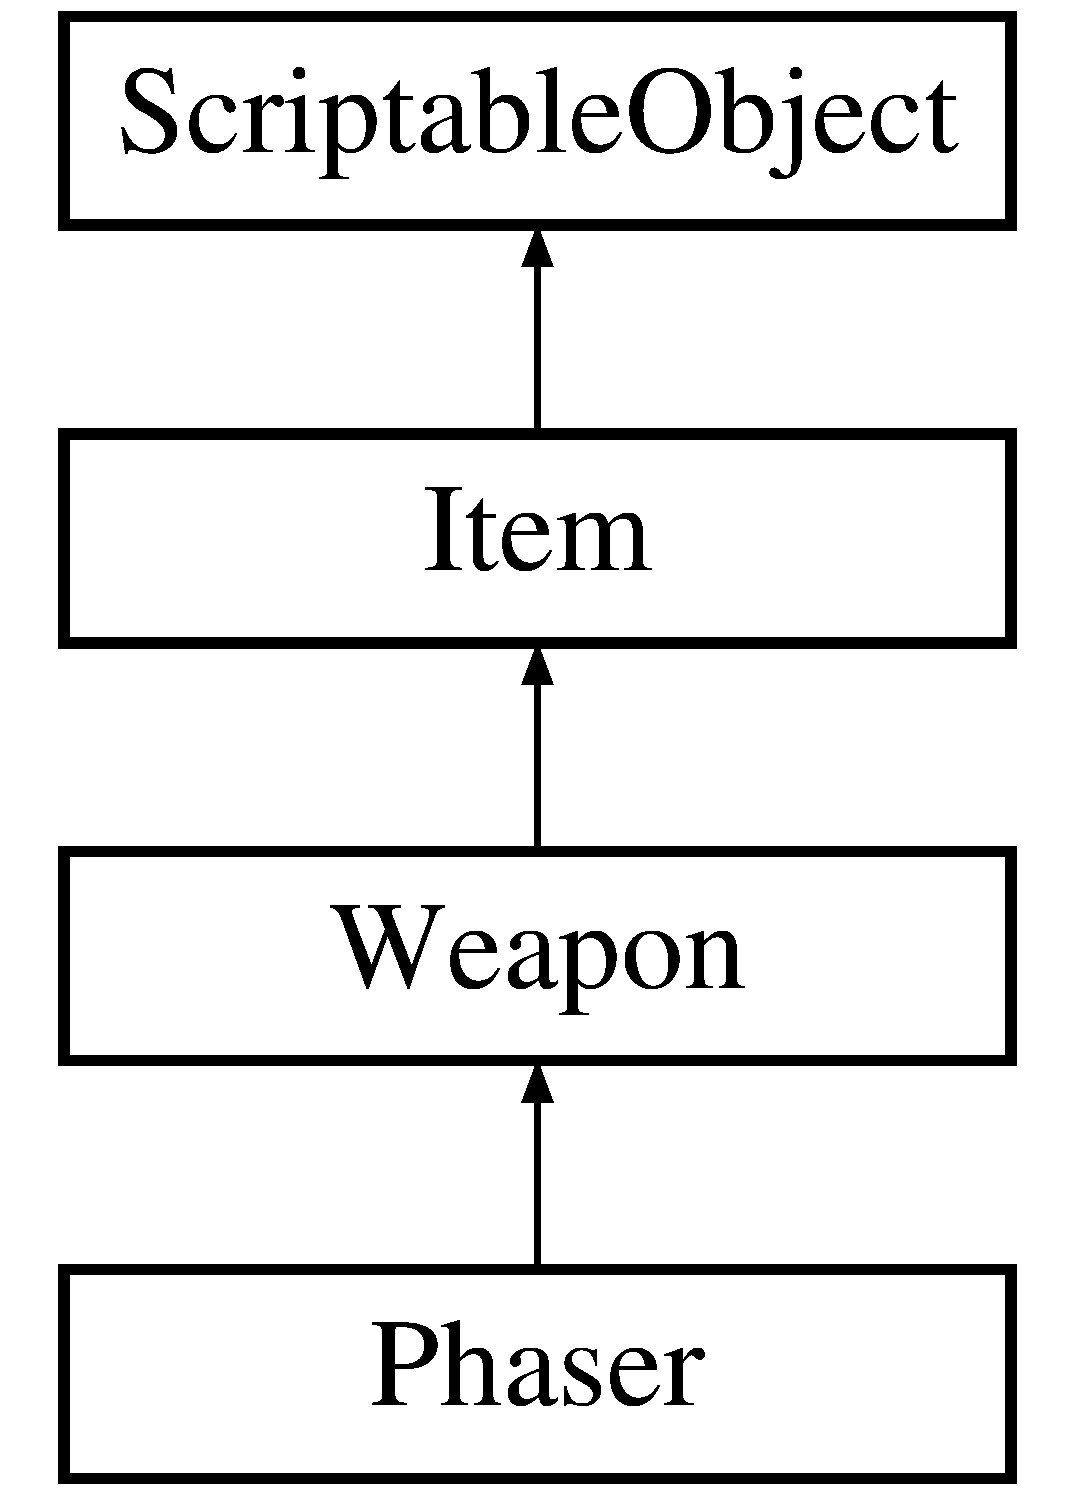
\includegraphics[height=4.000000cm]{class_phaser}
\end{center}
\end{figure}
\subsection*{Public Member Functions}
\begin{DoxyCompactItemize}
\item 
\mbox{\Hypertarget{class_phaser_afeed8f34e8d5424c4e397830e84d727b}\label{class_phaser_afeed8f34e8d5424c4e397830e84d727b}} 
\hyperlink{class_phaser}{Phaser} {\bfseries get\+\_\+copy} ()
\item 
\mbox{\Hypertarget{class_phaser_ac8038711b4e8e3a3685f2c798157300f}\label{class_phaser_ac8038711b4e8e3a3685f2c798157300f}} 
override void {\bfseries animation} ()
\item 
\mbox{\Hypertarget{class_phaser_a09b78147e6de56f0372eb07a88b99998}\label{class_phaser_a09b78147e6de56f0372eb07a88b99998}} 
override void {\bfseries deal\+\_\+damage} (int layer)
\end{DoxyCompactItemize}
\subsection*{Public Attributes}
\begin{DoxyCompactItemize}
\item 
\mbox{\Hypertarget{class_phaser_ae87e26eb87e4c22246b98ab5b5469c90}\label{class_phaser_ae87e26eb87e4c22246b98ab5b5469c90}} 
Phaser\+Type {\bfseries phaser\+\_\+type}
\item 
\mbox{\Hypertarget{class_phaser_addb890658bf4547fae53c61ba7503fa6}\label{class_phaser_addb890658bf4547fae53c61ba7503fa6}} 
Game\+Object {\bfseries start\+\_\+pos}
\item 
\mbox{\Hypertarget{class_phaser_a5665decd66dc4167e6e437ba0e0cdcc8}\label{class_phaser_a5665decd66dc4167e6e437ba0e0cdcc8}} 
Game\+Object {\bfseries end\+\_\+pos}
\item 
\mbox{\Hypertarget{class_phaser_ab5a677c4a5f5dcf4a669548f36d79423}\label{class_phaser_ab5a677c4a5f5dcf4a669548f36d79423}} 
float {\bfseries phaser\+\_\+anim\+\_\+lifetime} = 0.\+2f
\end{DoxyCompactItemize}
\subsection*{Additional Inherited Members}


The documentation for this class was generated from the following file\+:\begin{DoxyCompactItemize}
\item 
/\+Users/\+Leonard/\+Desktop/\+Stor\+Trok/\+Stor Trok/\+Assets/\+Stor Trok/\+Scripts/\+Items/\+Weapons/Phaser.\+cs\end{DoxyCompactItemize}

\hypertarget{class_phaser_type_module}{}\section{Phaser\+Type\+Module Class Reference}
\label{class_phaser_type_module}\index{Phaser\+Type\+Module@{Phaser\+Type\+Module}}
Inheritance diagram for Phaser\+Type\+Module\+:\begin{figure}[H]
\begin{center}
\leavevmode
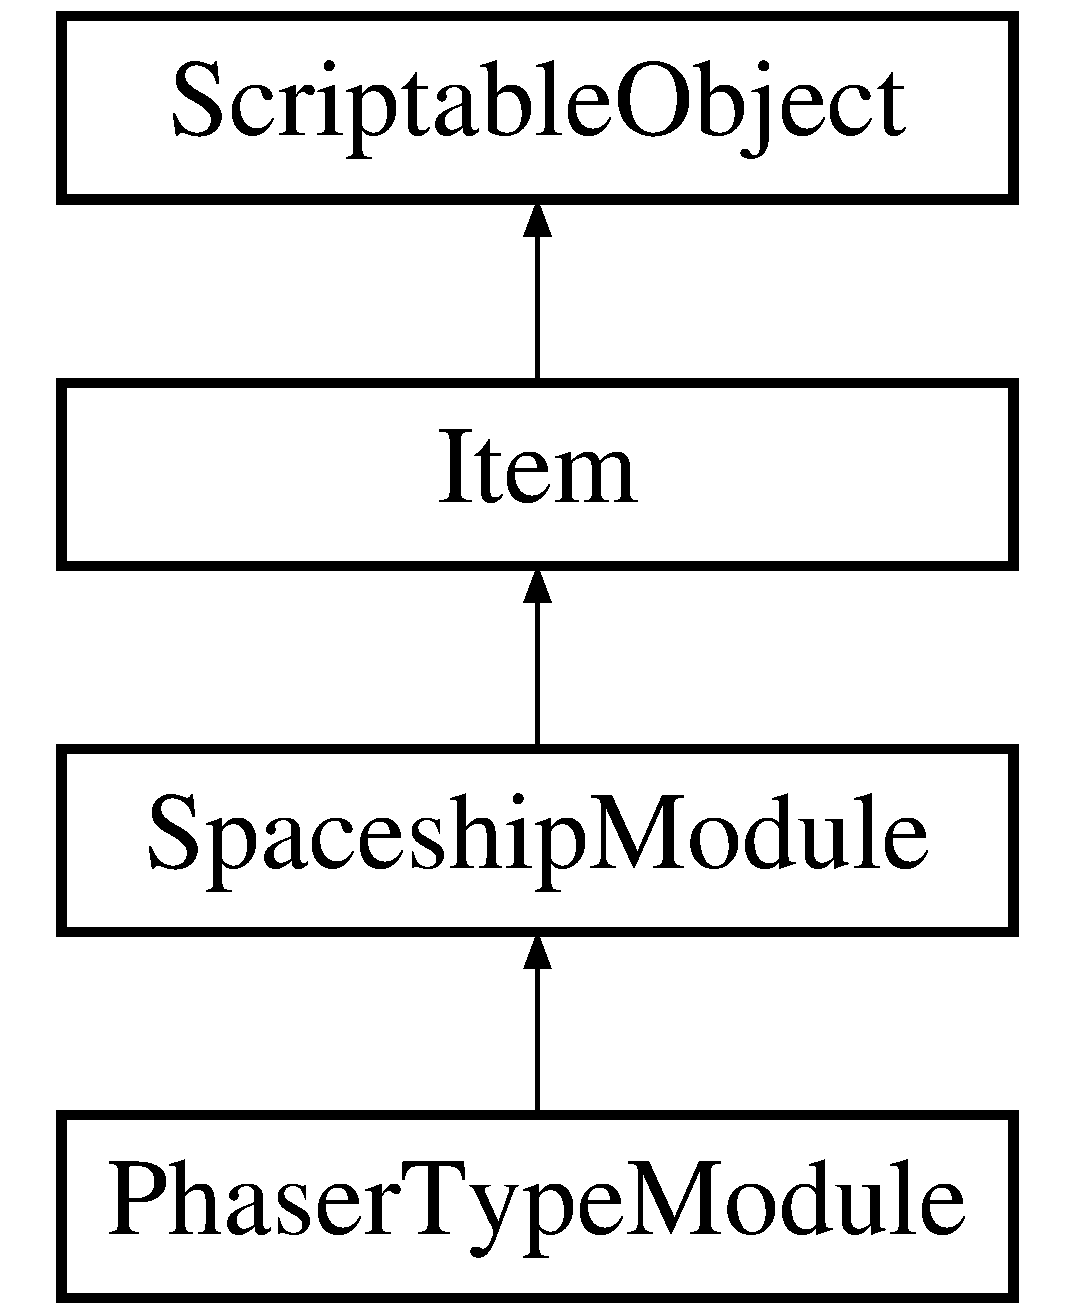
\includegraphics[height=4.000000cm]{class_phaser_type_module}
\end{center}
\end{figure}
\subsection*{Public Member Functions}
\begin{DoxyCompactItemize}
\item 
\mbox{\Hypertarget{class_phaser_type_module_a5eb7be4356bc7c8656a0a1c399911506}\label{class_phaser_type_module_a5eb7be4356bc7c8656a0a1c399911506}} 
override bool {\bfseries check\+\_\+effect} ()
\item 
\mbox{\Hypertarget{class_phaser_type_module_abc8c8e6fb18e6f44d115032b3ce9816c}\label{class_phaser_type_module_abc8c8e6fb18e6f44d115032b3ce9816c}} 
override void {\bfseries do\+\_\+effect} ()
\item 
\mbox{\Hypertarget{class_phaser_type_module_a3e4f570c93e6e1ddd274e92419030d30}\label{class_phaser_type_module_a3e4f570c93e6e1ddd274e92419030d30}} 
override void {\bfseries animation} ()
\end{DoxyCompactItemize}
\subsection*{Public Attributes}
\begin{DoxyCompactItemize}
\item 
\mbox{\Hypertarget{class_phaser_type_module_a8a91ad074d4bb8735e25b53fb31363f5}\label{class_phaser_type_module_a8a91ad074d4bb8735e25b53fb31363f5}} 
Color {\bfseries phaser\+\_\+beam\+\_\+color}
\end{DoxyCompactItemize}
\subsection*{Additional Inherited Members}


The documentation for this class was generated from the following file\+:\begin{DoxyCompactItemize}
\item 
/\+Users/\+Leonard/\+Desktop/\+Stor\+Trok/\+Stor Trok/\+Assets/\+Stor Trok/\+Scripts/\+Items/\+Spaceship\+Modules/Phaser\+Type\+Module.\+cs\end{DoxyCompactItemize}

\hypertarget{class_phaser_update}{}\section{Phaser\+Update Class Reference}
\label{class_phaser_update}\index{Phaser\+Update@{Phaser\+Update}}
Inheritance diagram for Phaser\+Update\+:\begin{figure}[H]
\begin{center}
\leavevmode
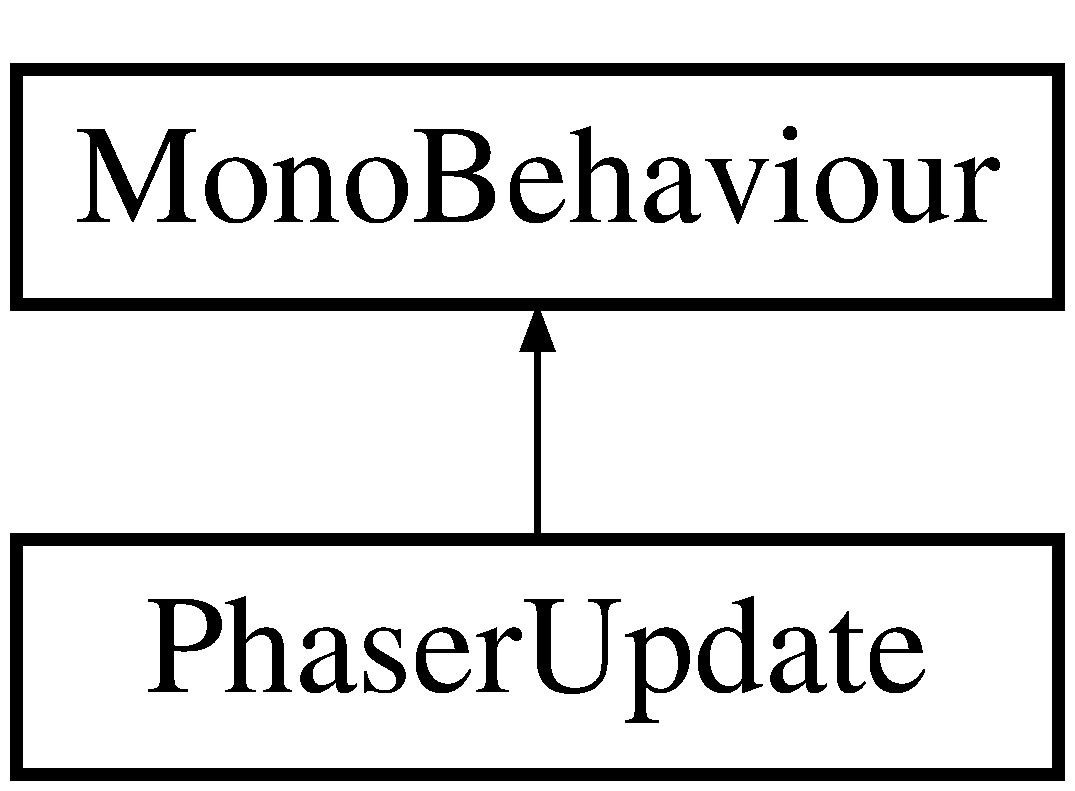
\includegraphics[height=2.000000cm]{class_phaser_update}
\end{center}
\end{figure}
\subsection*{Public Attributes}
\begin{DoxyCompactItemize}
\item 
\mbox{\Hypertarget{class_phaser_update_a6f83ab1e033f1275b7be520aab8217f0}\label{class_phaser_update_a6f83ab1e033f1275b7be520aab8217f0}} 
Game\+Object {\bfseries start\+\_\+pos}
\item 
\mbox{\Hypertarget{class_phaser_update_a716484ebe41feff50e05cf7445959351}\label{class_phaser_update_a716484ebe41feff50e05cf7445959351}} 
Game\+Object {\bfseries end\+\_\+pos}
\item 
\mbox{\Hypertarget{class_phaser_update_a312a36bd5a7009cc43085f946fe6be20}\label{class_phaser_update_a312a36bd5a7009cc43085f946fe6be20}} 
Line\+Renderer {\bfseries line\+\_\+renderer}
\item 
\mbox{\Hypertarget{class_phaser_update_a40e772cc7fed108a7e1a844a46140882}\label{class_phaser_update_a40e772cc7fed108a7e1a844a46140882}} 
Particle\+System {\bfseries ps}
\item 
\mbox{\Hypertarget{class_phaser_update_a382e0d3bbe954f03f6d02bfcddb0dc0a}\label{class_phaser_update_a382e0d3bbe954f03f6d02bfcddb0dc0a}} 
Particle\+System {\bfseries ps\+\_\+start\+\_\+effect}
\end{DoxyCompactItemize}


The documentation for this class was generated from the following file\+:\begin{DoxyCompactItemize}
\item 
/\+Users/\+Leonard/\+Desktop/\+Stor\+Trok/\+Stor Trok/\+Assets/\+Stor Trok/\+Scripts/\+Items/\+Weapons/Phaser\+Update.\+cs\end{DoxyCompactItemize}

\hypertarget{class_planet_system}{}\section{Planet\+System Class Reference}
\label{class_planet_system}\index{Planet\+System@{Planet\+System}}
Inheritance diagram for Planet\+System\+:\begin{figure}[H]
\begin{center}
\leavevmode
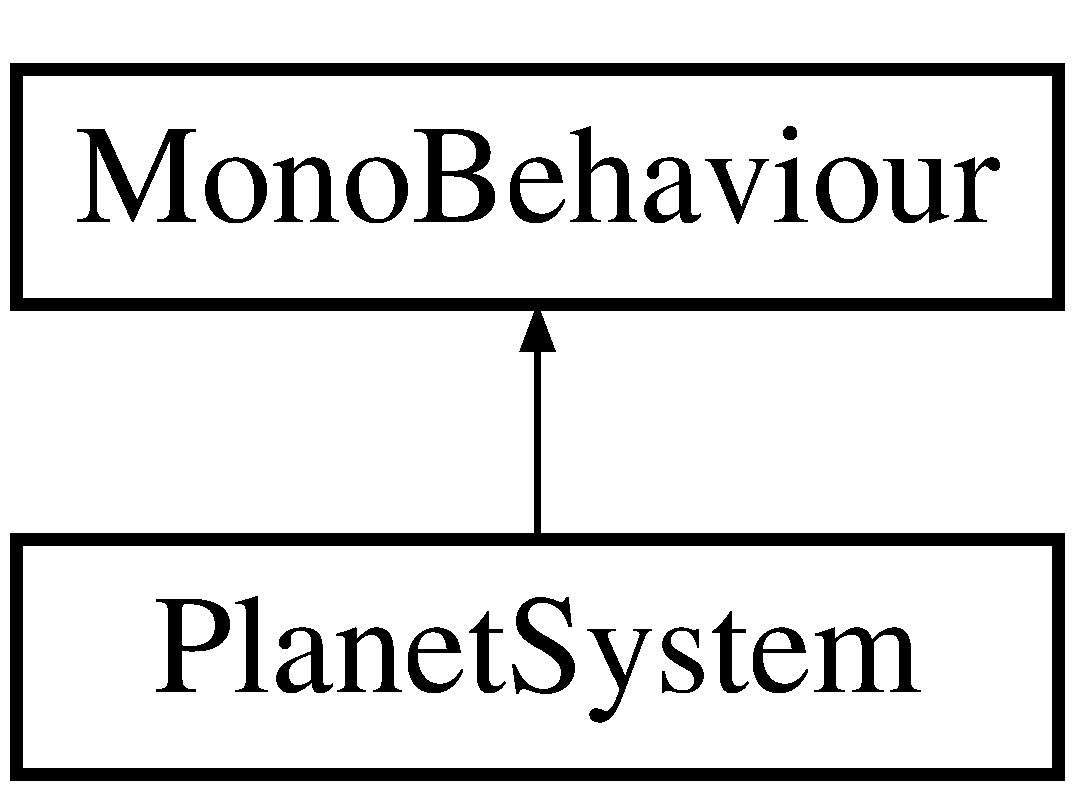
\includegraphics[height=2.000000cm]{class_planet_system}
\end{center}
\end{figure}
\subsection*{Public Attributes}
\begin{DoxyCompactItemize}
\item 
\mbox{\Hypertarget{class_planet_system_ad561d9c8c00e82b52a040e1211470ebe}\label{class_planet_system_ad561d9c8c00e82b52a040e1211470ebe}} 
\hyperlink{class_planet_system_data}{Planet\+System\+Data} {\bfseries system\+\_\+data}
\item 
\mbox{\Hypertarget{class_planet_system_a85d46b9451246456b9fab5964d300e6c}\label{class_planet_system_a85d46b9451246456b9fab5964d300e6c}} 
\hyperlink{class_object_aura}{Object\+Aura} {\bfseries object\+Aura}
\end{DoxyCompactItemize}
\subsection*{Properties}
\begin{DoxyCompactItemize}
\item 
\mbox{\Hypertarget{class_planet_system_a865ebeaf11a954f5cc7249935d055dfd}\label{class_planet_system_a865ebeaf11a954f5cc7249935d055dfd}} 
\hyperlink{class_mission_data}{Mission\+Data} {\bfseries mission\+\_\+data}\hspace{0.3cm}{\ttfamily  \mbox{[}get\mbox{]}}
\end{DoxyCompactItemize}


The documentation for this class was generated from the following file\+:\begin{DoxyCompactItemize}
\item 
/\+Users/\+Leonard/\+Desktop/\+Stor\+Trok/\+Stor Trok/\+Assets/\+Stor Trok/\+Scripts/\+Planet\+System/Planet\+System.\+cs\end{DoxyCompactItemize}

\hypertarget{class_planet_system_data}{}\section{Planet\+System\+Data Class Reference}
\label{class_planet_system_data}\index{Planet\+System\+Data@{Planet\+System\+Data}}
Inheritance diagram for Planet\+System\+Data\+:\begin{figure}[H]
\begin{center}
\leavevmode
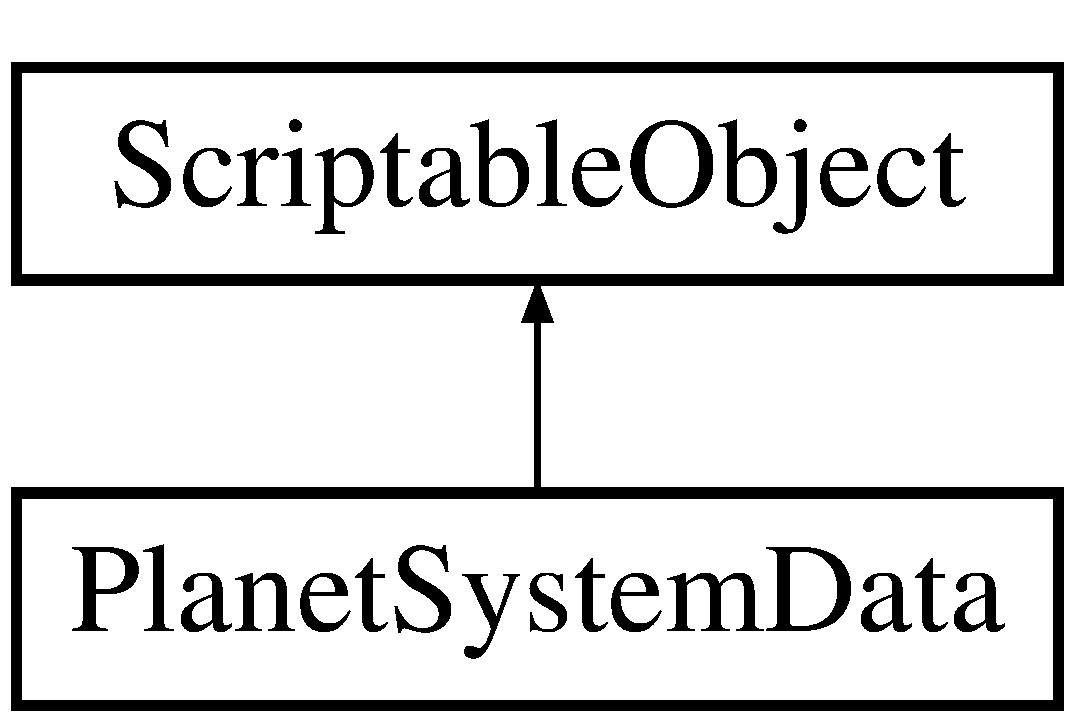
\includegraphics[height=2.000000cm]{class_planet_system_data}
\end{center}
\end{figure}
\subsection*{Static Public Member Functions}
\begin{DoxyCompactItemize}
\item 
\mbox{\Hypertarget{class_planet_system_data_ad92ecaaf1f3a93a73f31edf633d87295}\label{class_planet_system_data_ad92ecaaf1f3a93a73f31edf633d87295}} 
static \hyperlink{class_planet_system_data}{Planet\+System\+Data} {\bfseries get\+\_\+planet\+\_\+system\+\_\+data\+\_\+by\+\_\+id} (int id)
\end{DoxyCompactItemize}
\subsection*{Public Attributes}
\begin{DoxyCompactItemize}
\item 
\mbox{\Hypertarget{class_planet_system_data_ac1e0e0e22bf682d83e169a948e37e8de}\label{class_planet_system_data_ac1e0e0e22bf682d83e169a948e37e8de}} 
int {\bfseries ID}
\item 
\mbox{\Hypertarget{class_planet_system_data_aef5461cb330012608d4bc3a5b4ed339d}\label{class_planet_system_data_aef5461cb330012608d4bc3a5b4ed339d}} 
string {\bfseries system\+\_\+name}
\item 
\mbox{\Hypertarget{class_planet_system_data_ae2b9b4f5756e78728756ef8596742ac4}\label{class_planet_system_data_ae2b9b4f5756e78728756ef8596742ac4}} 
string {\bfseries description}
\item 
\mbox{\Hypertarget{class_planet_system_data_ae08111fb4983f8c692a4a9e0b6862467}\label{class_planet_system_data_ae08111fb4983f8c692a4a9e0b6862467}} 
string {\bfseries scene\+\_\+name}
\item 
\mbox{\Hypertarget{class_planet_system_data_a33dc9b9ccc32be44868a0a344925245d}\label{class_planet_system_data_a33dc9b9ccc32be44868a0a344925245d}} 
bool {\bfseries only\+\_\+mission} = false
\item 
\mbox{\Hypertarget{class_planet_system_data_a813c72e79956187c3ca88a31748b6d74}\label{class_planet_system_data_a813c72e79956187c3ca88a31748b6d74}} 
\hyperlink{class_mission_data}{Mission\+Data} {\bfseries mission\+\_\+data}
\end{DoxyCompactItemize}
\subsection*{Static Public Attributes}
\begin{DoxyCompactItemize}
\item 
\mbox{\Hypertarget{class_planet_system_data_a4c27b6dcfdf71b0786a5c735cb0ed5c8}\label{class_planet_system_data_a4c27b6dcfdf71b0786a5c735cb0ed5c8}} 
static List$<$ \hyperlink{class_planet_system_data}{Planet\+System\+Data} $>$ {\bfseries all\+\_\+planet\+\_\+systems} = new List$<$\hyperlink{class_planet_system_data}{Planet\+System\+Data}$>$()
\end{DoxyCompactItemize}


The documentation for this class was generated from the following file\+:\begin{DoxyCompactItemize}
\item 
/\+Users/\+Leonard/\+Desktop/\+Stor\+Trok/\+Stor Trok/\+Assets/\+Stor Trok/\+Scripts/\+Planet\+System/Planet\+System\+Data.\+cs\end{DoxyCompactItemize}

\hypertarget{class_player}{}\section{Player Class Reference}
\label{class_player}\index{Player@{Player}}
\subsection*{Public Member Functions}
\begin{DoxyCompactItemize}
\item 
\mbox{\Hypertarget{class_player_a3950af30aaf1ffc852fbd79a7c6f14d5}\label{class_player_a3950af30aaf1ffc852fbd79a7c6f14d5}} 
{\bfseries Player} (\hyperlink{class_spaceship}{Spaceship} s)
\item 
\mbox{\Hypertarget{class_player_aa9611f905a16638dba9c1873987fe4a9}\label{class_player_aa9611f905a16638dba9c1873987fe4a9}} 
{\bfseries Player} (Player\+Environment\+Status pes)
\item 
\mbox{\Hypertarget{class_player_a1f3a4cb09f5c8c885caf9583194bd16e}\label{class_player_a1f3a4cb09f5c8c885caf9583194bd16e}} 
void {\bfseries setup\+\_\+ship\+\_\+items} ()
\item 
\mbox{\Hypertarget{class_player_a249be50a7beb9083572a1c77b3271399}\label{class_player_a249be50a7beb9083572a1c77b3271399}} 
void {\bfseries setup\+\_\+modules} ()
\item 
\mbox{\Hypertarget{class_player_a9cddbe8840fa9a7a33ac0520765b4853}\label{class_player_a9cddbe8840fa9a7a33ac0520765b4853}} 
void {\bfseries setup\+\_\+weapons} ()
\item 
\mbox{\Hypertarget{class_player_a2ce7a482d9a6454f3278d052bcd02ef7}\label{class_player_a2ce7a482d9a6454f3278d052bcd02ef7}} 
void {\bfseries setup\+\_\+inventory} ()
\item 
\mbox{\Hypertarget{class_player_a4933c82202c7a7cef04717fcede6e5d9}\label{class_player_a4933c82202c7a7cef04717fcede6e5d9}} 
void {\bfseries setup\+\_\+antrieb} ()
\item 
\mbox{\Hypertarget{class_player_aabb5c185405b3f77747447918dec94b5}\label{class_player_aabb5c185405b3f77747447918dec94b5}} 
void {\bfseries setup\+\_\+schild} ()
\item 
\mbox{\Hypertarget{class_player_a29ccabb89925e1d4ef80e28a2b7da8e9}\label{class_player_a29ccabb89925e1d4ef80e28a2b7da8e9}} 
List$<$ \hyperlink{class_weapon}{Weapon} $>$ {\bfseries get\+\_\+top\+\_\+weapons} ()
\item 
\mbox{\Hypertarget{class_player_a6db9aa013dbb55802bce008b363490e0}\label{class_player_a6db9aa013dbb55802bce008b363490e0}} 
List$<$ \hyperlink{class_weapon}{Weapon} $>$ {\bfseries get\+\_\+bot\+\_\+weapons} ()
\item 
\mbox{\Hypertarget{class_player_a8708e99901002a2e5fe9e4b0a32459f5}\label{class_player_a8708e99901002a2e5fe9e4b0a32459f5}} 
\hyperlink{class_spaceship_weapon_position}{Spaceship\+Weapon\+Position} {\bfseries get\+\_\+top\+\_\+weapon\+\_\+position} ()
\item 
\mbox{\Hypertarget{class_player_afb7246586bfac930d9c026f0ce4d82f4}\label{class_player_afb7246586bfac930d9c026f0ce4d82f4}} 
\hyperlink{class_spaceship_weapon_position}{Spaceship\+Weapon\+Position} {\bfseries get\+\_\+bot\+\_\+weapon\+\_\+position} ()
\end{DoxyCompactItemize}
\subsection*{Public Attributes}
\begin{DoxyCompactItemize}
\item 
\mbox{\Hypertarget{class_player_ad4c2ab5c71c359ab76459daa397c4614}\label{class_player_ad4c2ab5c71c359ab76459daa397c4614}} 
const int {\bfseries environment\+\_\+layer} = 10
\item 
\mbox{\Hypertarget{class_player_af674941521cbd725210217e204ad7a99}\label{class_player_af674941521cbd725210217e204ad7a99}} 
const int {\bfseries player\+\_\+layer} = 9
\item 
\mbox{\Hypertarget{class_player_a5a5b105285ae9d74073d58dd8dc94fb5}\label{class_player_a5a5b105285ae9d74073d58dd8dc94fb5}} 
const int {\bfseries enemy\+\_\+layer} = 8
\item 
\mbox{\Hypertarget{class_player_ac8bcb50bf826874dfa2d162af367d013}\label{class_player_ac8bcb50bf826874dfa2d162af367d013}} 
string {\bfseries name}
\item 
\mbox{\Hypertarget{class_player_aed37167e4117c2518a154e73fbfc103c}\label{class_player_aed37167e4117c2518a154e73fbfc103c}} 
int {\bfseries money}
\item 
\mbox{\Hypertarget{class_player_a0e958a88a824f08873837fcf7d22344b}\label{class_player_a0e958a88a824f08873837fcf7d22344b}} 
\hyperlink{class_spaceship}{Spaceship} {\bfseries spaceship}
\item 
\mbox{\Hypertarget{class_player_a27e922aea5e6371a33c0fa97e10413cd}\label{class_player_a27e922aea5e6371a33c0fa97e10413cd}} 
Player\+Environment\+Status {\bfseries player\+\_\+environment\+\_\+status} = Player\+Environment\+Status.\+None
\item 
\mbox{\Hypertarget{class_player_a333843d71092ceb812d2f2715e6a20fa}\label{class_player_a333843d71092ceb812d2f2715e6a20fa}} 
\hyperlink{class_inventar}{Inventar} {\bfseries player\+\_\+inventar}
\item 
\mbox{\Hypertarget{class_player_a8cd10622dac298adaa763e6ae853e9a5}\label{class_player_a8cd10622dac298adaa763e6ae853e9a5}} 
Vector3 {\bfseries last\+\_\+coordinate}
\end{DoxyCompactItemize}
\subsection*{Properties}
\begin{DoxyCompactItemize}
\item 
\mbox{\Hypertarget{class_player_ac7317ab15537dffd0222fc019fe28c5e}\label{class_player_ac7317ab15537dffd0222fc019fe28c5e}} 
string {\bfseries player\+\_\+data\+\_\+path}\hspace{0.3cm}{\ttfamily  \mbox{[}get\mbox{]}}
\item 
\mbox{\Hypertarget{class_player_a626d7b1a0a69ccb17979ea7a0728fca7}\label{class_player_a626d7b1a0a69ccb17979ea7a0728fca7}} 
static \hyperlink{class_player}{Player} {\bfseries player}\hspace{0.3cm}{\ttfamily  \mbox{[}get, set\mbox{]}}
\end{DoxyCompactItemize}


The documentation for this class was generated from the following file\+:\begin{DoxyCompactItemize}
\item 
/\+Users/\+Leonard/\+Desktop/\+Stor\+Trok/\+Stor Trok/\+Assets/\+Stor Trok/\+Scripts/\+Player/Player.\+cs\end{DoxyCompactItemize}

\hypertarget{class_player_data}{}\section{Player\+Data Class Reference}
\label{class_player_data}\index{Player\+Data@{Player\+Data}}
\subsection*{Public Member Functions}
\begin{DoxyCompactItemize}
\item 
\mbox{\Hypertarget{class_player_data_a691f1547f6a37b84fdea47ca0dd52442}\label{class_player_data_a691f1547f6a37b84fdea47ca0dd52442}} 
\hyperlink{class_spaceship_data}{Spaceship\+Data} {\bfseries get\+\_\+current\+\_\+spaceship} ()
\item 
\mbox{\Hypertarget{class_player_data_aa0698be7705e842f89f2446efa9a6697}\label{class_player_data_aa0698be7705e842f89f2446efa9a6697}} 
void {\bfseries add\+\_\+spaceship} (int id)
\item 
\mbox{\Hypertarget{class_player_data_af76e093858c19962061cf698fd8ba51f}\label{class_player_data_af76e093858c19962061cf698fd8ba51f}} 
void {\bfseries set\+\_\+ids} ()
\end{DoxyCompactItemize}
\subsection*{Static Public Member Functions}
\begin{DoxyCompactItemize}
\item 
\mbox{\Hypertarget{class_player_data_ad4848c807b599800703d778afd12409e}\label{class_player_data_ad4848c807b599800703d778afd12409e}} 
static \hyperlink{class_player_data}{Player\+Data} {\bfseries new\+\_\+player} (int spaceship\+\_\+id)
\end{DoxyCompactItemize}
\subsection*{Public Attributes}
\begin{DoxyCompactItemize}
\item 
\mbox{\Hypertarget{class_player_data_a5b74be3f2b0098e0eeaa7e2603be0910}\label{class_player_data_a5b74be3f2b0098e0eeaa7e2603be0910}} 
string {\bfseries name}
\item 
\mbox{\Hypertarget{class_player_data_a961f68b58c5bae23ae356114e2ac093f}\label{class_player_data_a961f68b58c5bae23ae356114e2ac093f}} 
int {\bfseries money}
\item 
\mbox{\Hypertarget{class_player_data_a727a94961f2bc63757ecca9a3345a467}\label{class_player_data_a727a94961f2bc63757ecca9a3345a467}} 
List$<$ int $>$ {\bfseries inventar}
\item 
\mbox{\Hypertarget{class_player_data_a2ee6f73a86bcaed440d8e83849bd3063}\label{class_player_data_a2ee6f73a86bcaed440d8e83849bd3063}} 
int {\bfseries selected\+\_\+item}
\item 
\mbox{\Hypertarget{class_player_data_ab308180ee785d2f35ea745a380cb6276}\label{class_player_data_ab308180ee785d2f35ea745a380cb6276}} 
List$<$ \hyperlink{class_spaceship_data}{Spaceship\+Data} $>$ {\bfseries owned\+\_\+spaceships\+\_\+with\+\_\+items}
\item 
\mbox{\Hypertarget{class_player_data_a2ee8dc2318b050e7aae9e380ac4ce502}\label{class_player_data_a2ee8dc2318b050e7aae9e380ac4ce502}} 
int {\bfseries current\+\_\+spaceship}
\item 
\mbox{\Hypertarget{class_player_data_a59f5422266dac7e8ee6483b52733cd3a}\label{class_player_data_a59f5422266dac7e8ee6483b52733cd3a}} 
\hyperlink{class_serializable_vector3}{Serializable\+Vector3} {\bfseries sektorenraum\+\_\+koordinaten}
\end{DoxyCompactItemize}


The documentation for this class was generated from the following file\+:\begin{DoxyCompactItemize}
\item 
/\+Users/\+Leonard/\+Desktop/\+Stor\+Trok/\+Stor Trok/\+Assets/\+Stor Trok/\+Scripts/\+Data/Player\+Data.\+cs\end{DoxyCompactItemize}

\hypertarget{class_player_movement_data}{}\section{Player\+Movement\+Data Class Reference}
\label{class_player_movement_data}\index{Player\+Movement\+Data@{Player\+Movement\+Data}}
\subsection*{Public Member Functions}
\begin{DoxyCompactItemize}
\item 
\mbox{\Hypertarget{class_player_movement_data_a556692307eab67f2528d6edc75ee255e}\label{class_player_movement_data_a556692307eab67f2528d6edc75ee255e}} 
float {\bfseries compare\+\_\+player\+\_\+movement\+\_\+data} (\hyperlink{class_player_movement_data}{Player\+Movement\+Data} data)
\item 
\mbox{\Hypertarget{class_player_movement_data_adf2202ac5170a973c9c1b97912dbb729}\label{class_player_movement_data_adf2202ac5170a973c9c1b97912dbb729}} 
float {\bfseries compare\+\_\+player\+\_\+movement\+\_\+data} (\hyperlink{struct_spaceship_relative_situation}{Spaceship\+Relative\+Situation} sit)
\end{DoxyCompactItemize}
\subsection*{Static Public Member Functions}
\begin{DoxyCompactItemize}
\item 
\mbox{\Hypertarget{class_player_movement_data_aa9fa3555b33a189ce426a49879af54bd}\label{class_player_movement_data_aa9fa3555b33a189ce426a49879af54bd}} 
static void {\bfseries load\+\_\+data\+\_\+set} ()
\item 
\mbox{\Hypertarget{class_player_movement_data_ae81023938fbf2a0ce9491dd96820bb62}\label{class_player_movement_data_ae81023938fbf2a0ce9491dd96820bb62}} 
static void {\bfseries save\+\_\+data\+\_\+set} ()
\item 
\mbox{\Hypertarget{class_player_movement_data_ace02d521d186f7d02a74303334c73b27}\label{class_player_movement_data_ace02d521d186f7d02a74303334c73b27}} 
static float {\bfseries compare\+\_\+player\+\_\+movement\+\_\+data} (\hyperlink{class_player_movement_data}{Player\+Movement\+Data} data1, \hyperlink{class_player_movement_data}{Player\+Movement\+Data} data2)
\item 
\mbox{\Hypertarget{class_player_movement_data_aa732dca43740f2acfac56b44e0ea8867}\label{class_player_movement_data_aa732dca43740f2acfac56b44e0ea8867}} 
static \hyperlink{class_player_movement_data}{Player\+Movement\+Data} {\bfseries find\+\_\+best\+\_\+match} (\hyperlink{struct_spaceship_relative_situation}{Spaceship\+Relative\+Situation} situation)
\end{DoxyCompactItemize}
\subsection*{Public Attributes}
\begin{DoxyCompactItemize}
\item 
\mbox{\Hypertarget{class_player_movement_data_a8ffd04d401c12c78b4f0faae28d4c7a1}\label{class_player_movement_data_a8ffd04d401c12c78b4f0faae28d4c7a1}} 
\hyperlink{struct_spaceship_input}{Spaceship\+Input} {\bfseries player\+\_\+input}
\item 
\mbox{\Hypertarget{class_player_movement_data_a81065ba299bbe187ec345b043f91c2ac}\label{class_player_movement_data_a81065ba299bbe187ec345b043f91c2ac}} 
\hyperlink{struct_spaceship_relative_situation}{Spaceship\+Relative\+Situation} {\bfseries player\+\_\+situation}
\end{DoxyCompactItemize}
\subsection*{Static Public Attributes}
\begin{DoxyCompactItemize}
\item 
\mbox{\Hypertarget{class_player_movement_data_a98f5de3bbb2a48db0d93b482795adb19}\label{class_player_movement_data_a98f5de3bbb2a48db0d93b482795adb19}} 
static List$<$ \hyperlink{class_player_movement_data}{Player\+Movement\+Data} $>$ {\bfseries data\+\_\+set} = new List$<$\hyperlink{class_player_movement_data}{Player\+Movement\+Data}$>$()
\item 
\mbox{\Hypertarget{class_player_movement_data_a883aa9f57c92034fc7e6d3035c3b5594}\label{class_player_movement_data_a883aa9f57c92034fc7e6d3035c3b5594}} 
static string {\bfseries data\+\_\+path}
\item 
\mbox{\Hypertarget{class_player_movement_data_a5cb0febb79c8e131ccd5ce220706f69c}\label{class_player_movement_data_a5cb0febb79c8e131ccd5ce220706f69c}} 
static bool {\bfseries data\+\_\+set\+\_\+loaded} = false
\end{DoxyCompactItemize}


The documentation for this class was generated from the following file\+:\begin{DoxyCompactItemize}
\item 
/\+Users/\+Leonard/\+Desktop/\+Stor\+Trok/\+Stor Trok/\+Assets/\+Stor Trok/\+Scripts/\+Computer\+Players/\+Movement\+Types/\+Movement\+With\+Player\+Data/Player\+Movement\+Data.\+cs\end{DoxyCompactItemize}

\hypertarget{class_player_script}{}\section{Player\+Script Class Reference}
\label{class_player_script}\index{Player\+Script@{Player\+Script}}
Inheritance diagram for Player\+Script\+:\begin{figure}[H]
\begin{center}
\leavevmode
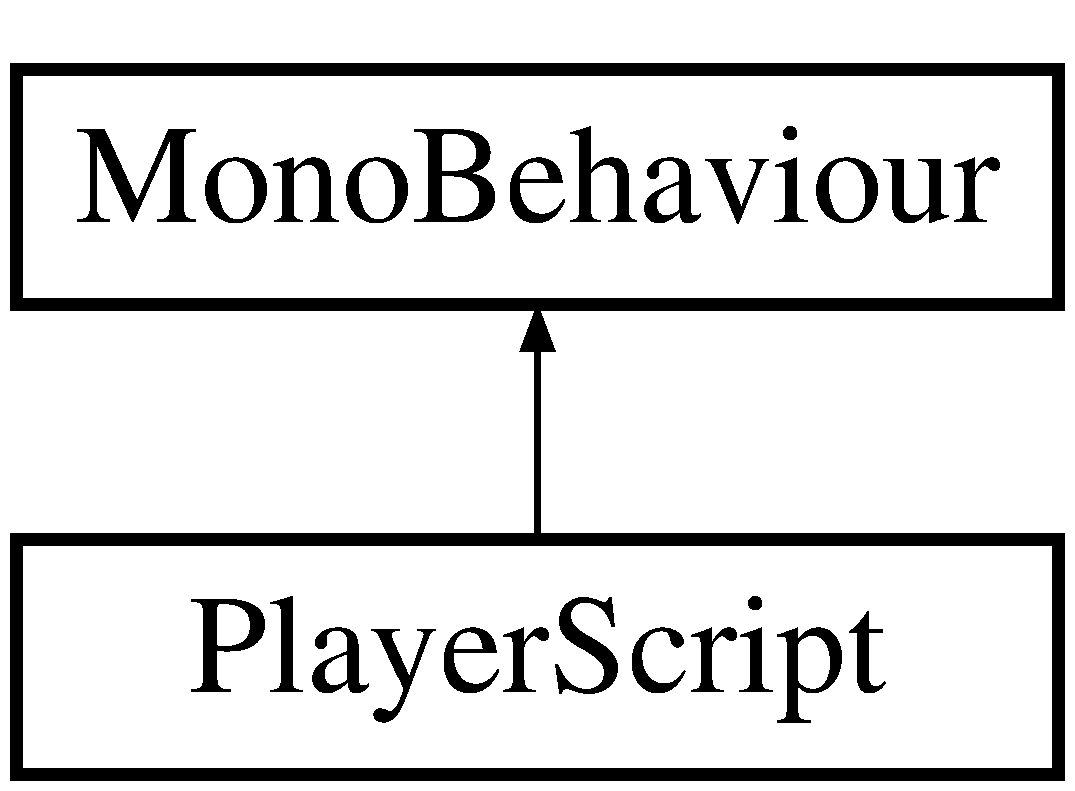
\includegraphics[height=2.000000cm]{class_player_script}
\end{center}
\end{figure}
\subsection*{Public Member Functions}
\begin{DoxyCompactItemize}
\item 
\mbox{\Hypertarget{class_player_script_a8376bbed9a07f2d4596b747a20bf56f4}\label{class_player_script_a8376bbed9a07f2d4596b747a20bf56f4}} 
\hyperlink{class_spaceship}{Spaceship} {\bfseries get\+\_\+enemy} ()
\item 
\mbox{\Hypertarget{class_player_script_a238dd91e487e0402feedc419e6476904}\label{class_player_script_a238dd91e487e0402feedc419e6476904}} 
void {\bfseries attack\+\_\+enemy} ()
\item 
\mbox{\Hypertarget{class_player_script_a318bf10363985f6fbd6566d04534353e}\label{class_player_script_a318bf10363985f6fbd6566d04534353e}} 
void {\bfseries attack\+\_\+input} ()
\end{DoxyCompactItemize}
\subsection*{Public Attributes}
\begin{DoxyCompactItemize}
\item 
\mbox{\Hypertarget{class_player_script_a26145e1e84e3277b10d11403ac290066}\label{class_player_script_a26145e1e84e3277b10d11403ac290066}} 
\hyperlink{class_spaceship}{Spaceship} {\bfseries spaceship}
\item 
\mbox{\Hypertarget{class_player_script_af343886e3367dddb1565ffe8b87c4263}\label{class_player_script_af343886e3367dddb1565ffe8b87c4263}} 
bool {\bfseries mobile\+\_\+input} = false
\item 
\mbox{\Hypertarget{class_player_script_a8c02dfebc64588743115f9906d0e2bb7}\label{class_player_script_a8c02dfebc64588743115f9906d0e2bb7}} 
Game\+Object {\bfseries selected\+\_\+enemy}
\item 
\mbox{\Hypertarget{class_player_script_a610149a1f9da9199e42edd2d16d90e9e}\label{class_player_script_a610149a1f9da9199e42edd2d16d90e9e}} 
Weapon\+Raw\+Types {\bfseries weapon\+\_\+types} = Weapon\+Raw\+Types.\+None
\end{DoxyCompactItemize}
\subsection*{Static Public Attributes}
\begin{DoxyCompactItemize}
\item 
\mbox{\Hypertarget{class_player_script_af394b88c93e6724670fdd830c867a78b}\label{class_player_script_af394b88c93e6724670fdd830c867a78b}} 
static \hyperlink{class_player_script}{Player\+Script} {\bfseries player\+Script}
\end{DoxyCompactItemize}


The documentation for this class was generated from the following file\+:\begin{DoxyCompactItemize}
\item 
/\+Users/\+Leonard/\+Desktop/\+Stor\+Trok/\+Stor Trok/\+Assets/\+Stor Trok/\+Scripts/\+Player/Player\+Script.\+cs\end{DoxyCompactItemize}

\hypertarget{class_puls_phaser}{}\section{Puls\+Phaser Class Reference}
\label{class_puls_phaser}\index{Puls\+Phaser@{Puls\+Phaser}}
Inheritance diagram for Puls\+Phaser\+:\begin{figure}[H]
\begin{center}
\leavevmode
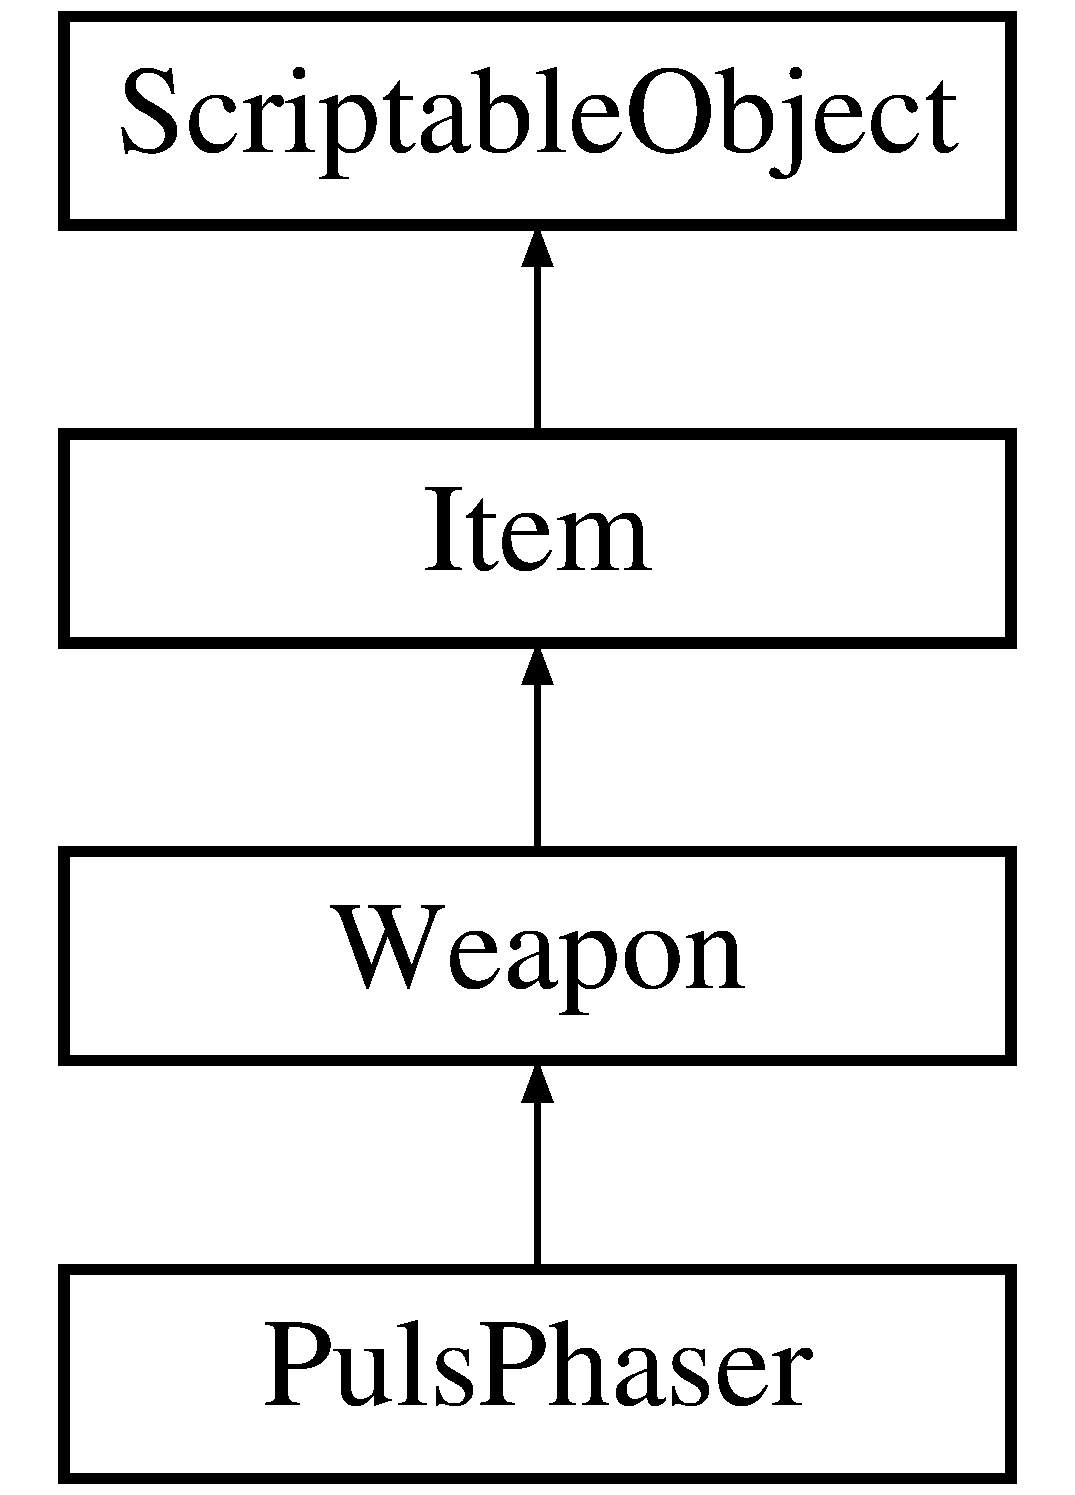
\includegraphics[height=4.000000cm]{class_puls_phaser}
\end{center}
\end{figure}
\subsection*{Public Member Functions}
\begin{DoxyCompactItemize}
\item 
\mbox{\Hypertarget{class_puls_phaser_a9cefce37a960081cf96620952792cd0d}\label{class_puls_phaser_a9cefce37a960081cf96620952792cd0d}} 
override bool {\bfseries can\+\_\+shoot} ()
\item 
\mbox{\Hypertarget{class_puls_phaser_ad6e860eb4808d833ef314a4cc012e02e}\label{class_puls_phaser_ad6e860eb4808d833ef314a4cc012e02e}} 
override void {\bfseries shoot} ()
\item 
\mbox{\Hypertarget{class_puls_phaser_aef7ade6c674edf931cf5fd00262d3b6d}\label{class_puls_phaser_aef7ade6c674edf931cf5fd00262d3b6d}} 
override void {\bfseries animation} ()
\item 
\mbox{\Hypertarget{class_puls_phaser_a95cfb2398e2e6fc217833c0e0845ee98}\label{class_puls_phaser_a95cfb2398e2e6fc217833c0e0845ee98}} 
override void {\bfseries deal\+\_\+damage} (int layer)
\end{DoxyCompactItemize}
\subsection*{Public Attributes}
\begin{DoxyCompactItemize}
\item 
\mbox{\Hypertarget{class_puls_phaser_a4de6f49e6f25e894804d4445b009b476}\label{class_puls_phaser_a4de6f49e6f25e894804d4445b009b476}} 
Puls\+Phaser\+Type {\bfseries puls\+\_\+phaser\+\_\+type}
\item 
\mbox{\Hypertarget{class_puls_phaser_a103a91e5a6c4b08b2bcc9c2e26aaba85}\label{class_puls_phaser_a103a91e5a6c4b08b2bcc9c2e26aaba85}} 
Game\+Object {\bfseries target\+\_\+object}
\item 
\mbox{\Hypertarget{class_puls_phaser_ab90dff5bc0e667619ee8c060b9fce547}\label{class_puls_phaser_ab90dff5bc0e667619ee8c060b9fce547}} 
int {\bfseries enemy\+\_\+layer}
\item 
\mbox{\Hypertarget{class_puls_phaser_ac54bdede3eaeb9e388a87270d277bb47}\label{class_puls_phaser_ac54bdede3eaeb9e388a87270d277bb47}} 
int {\bfseries salve\+\_\+size}
\item 
\mbox{\Hypertarget{class_puls_phaser_aa82b6f0ca30e589c0ef54a51244b944e}\label{class_puls_phaser_aa82b6f0ca30e589c0ef54a51244b944e}} 
float {\bfseries salve\+\_\+reload\+\_\+time}
\item 
\mbox{\Hypertarget{class_puls_phaser_aab30bccc3e64d9ba26f75b20e59f7c05}\label{class_puls_phaser_aab30bccc3e64d9ba26f75b20e59f7c05}} 
bool {\bfseries single}
\item 
\mbox{\Hypertarget{class_puls_phaser_aec1223f2f87386a2c2cab63cdddc9cee}\label{class_puls_phaser_aec1223f2f87386a2c2cab63cdddc9cee}} 
int {\bfseries missiles\+\_\+shot} = 0
\end{DoxyCompactItemize}
\subsection*{Additional Inherited Members}


The documentation for this class was generated from the following file\+:\begin{DoxyCompactItemize}
\item 
/\+Users/\+Leonard/\+Desktop/\+Stor\+Trok/\+Stor Trok/\+Assets/\+Stor Trok/\+Scripts/\+Items/\+Weapons/Puls\+Phaser.\+cs\end{DoxyCompactItemize}

\hypertarget{class_puls_phaser_update}{}\section{Puls\+Phaser\+Update Class Reference}
\label{class_puls_phaser_update}\index{Puls\+Phaser\+Update@{Puls\+Phaser\+Update}}
Inheritance diagram for Puls\+Phaser\+Update\+:\begin{figure}[H]
\begin{center}
\leavevmode
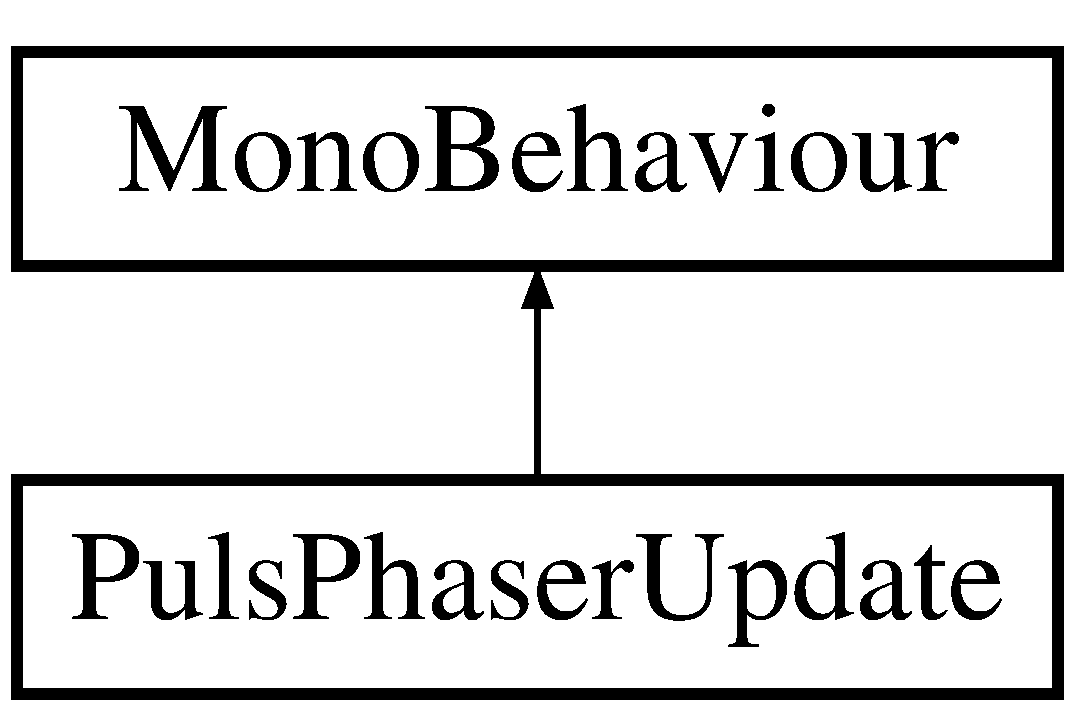
\includegraphics[height=2.000000cm]{class_puls_phaser_update}
\end{center}
\end{figure}
\subsection*{Public Attributes}
\begin{DoxyCompactItemize}
\item 
\mbox{\Hypertarget{class_puls_phaser_update_aa5f113fb36900f4914ca0ac6ec623571}\label{class_puls_phaser_update_aa5f113fb36900f4914ca0ac6ec623571}} 
Game\+Object {\bfseries target}
\item 
\mbox{\Hypertarget{class_puls_phaser_update_a1314b5312eba2c77d6376c59d0123b66}\label{class_puls_phaser_update_a1314b5312eba2c77d6376c59d0123b66}} 
int {\bfseries enemy\+\_\+layer}
\item 
\mbox{\Hypertarget{class_puls_phaser_update_a5daed4a568c876f048c2297a092a1ece}\label{class_puls_phaser_update_a5daed4a568c876f048c2297a092a1ece}} 
\hyperlink{class_puls_phaser}{Puls\+Phaser} {\bfseries puls\+\_\+phaser}
\item 
\mbox{\Hypertarget{class_puls_phaser_update_a6d695a148326c176797af6d40badb9e3}\label{class_puls_phaser_update_a6d695a148326c176797af6d40badb9e3}} 
const float {\bfseries speed} = 800
\item 
\mbox{\Hypertarget{class_puls_phaser_update_a29163d6cf8dedf7395551f8f1d764ff8}\label{class_puls_phaser_update_a29163d6cf8dedf7395551f8f1d764ff8}} 
const float {\bfseries life\+\_\+time} = 10
\end{DoxyCompactItemize}


The documentation for this class was generated from the following file\+:\begin{DoxyCompactItemize}
\item 
/\+Users/\+Leonard/\+Desktop/\+Stor\+Trok/\+Stor Trok/\+Assets/\+Stor Trok/\+Scripts/\+Items/\+Weapons/Puls\+Phaser\+Update.\+cs\end{DoxyCompactItemize}

\hypertarget{class_range}{}\section{Range Class Reference}
\label{class_range}\index{Range@{Range}}
\subsection*{Public Member Functions}
\begin{DoxyCompactItemize}
\item 
\mbox{\Hypertarget{class_range_a870d4c20c77fd12d570660f82935a79b}\label{class_range_a870d4c20c77fd12d570660f82935a79b}} 
{\bfseries Range} (float min, float max)
\item 
\mbox{\Hypertarget{class_range_a68f1b9a17e2c21135b02e7c994124ae5}\label{class_range_a68f1b9a17e2c21135b02e7c994124ae5}} 
bool {\bfseries contains\+\_\+number} (float number)
\end{DoxyCompactItemize}
\subsection*{Public Attributes}
\begin{DoxyCompactItemize}
\item 
\mbox{\Hypertarget{class_range_aa1bddd6f00ebcda6aa9243973917b401}\label{class_range_aa1bddd6f00ebcda6aa9243973917b401}} 
float {\bfseries min}
\item 
\mbox{\Hypertarget{class_range_a8d499f125609ce8b0d13fa0d50da840b}\label{class_range_a8d499f125609ce8b0d13fa0d50da840b}} 
float {\bfseries max}
\end{DoxyCompactItemize}
\subsection*{Properties}
\begin{DoxyCompactItemize}
\item 
\mbox{\Hypertarget{class_range_a0e72f09a41f80baa93820834456bdb62}\label{class_range_a0e72f09a41f80baa93820834456bdb62}} 
float {\bfseries medium}\hspace{0.3cm}{\ttfamily  \mbox{[}get\mbox{]}}
\end{DoxyCompactItemize}


The documentation for this class was generated from the following file\+:\begin{DoxyCompactItemize}
\item 
/\+Users/\+Leonard/\+Desktop/\+Stor\+Trok/\+Stor Trok/\+Assets/\+Stor Trok/\+Scripts/Utils.\+cs\end{DoxyCompactItemize}

\hypertarget{class_raumschiff}{}\section{Raumschiff Class Reference}
\label{class_raumschiff}\index{Raumschiff@{Raumschiff}}
Inheritance diagram for Raumschiff\+:\begin{figure}[H]
\begin{center}
\leavevmode
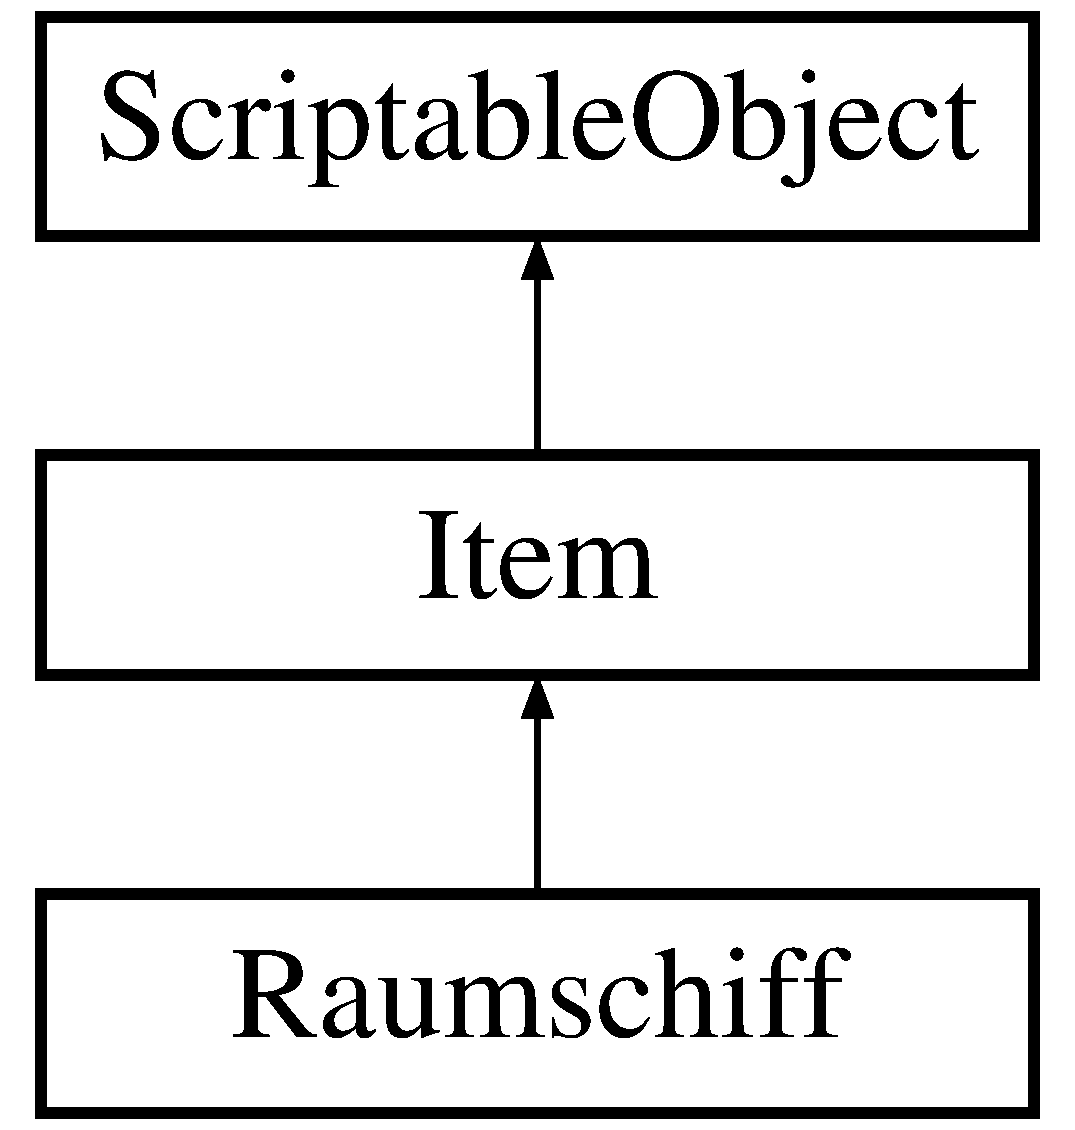
\includegraphics[height=3.000000cm]{class_raumschiff}
\end{center}
\end{figure}
\subsection*{Public Member Functions}
\begin{DoxyCompactItemize}
\item 
override string \hyperlink{class_raumschiff_a9aa65a7d3deb846709b85be4d157d621}{get\+\_\+description\+\_\+text} ()
\begin{DoxyCompactList}\small\item\em Erstellt einen Text, der im \hyperlink{class_inventar}{Inventar} angezeigt wird, wenn der Mauszeiger auf dem \hyperlink{class_item}{Item} ist \end{DoxyCompactList}\end{DoxyCompactItemize}
\subsection*{Static Public Member Functions}
\begin{DoxyCompactItemize}
\item 
\mbox{\Hypertarget{class_raumschiff_aa783459dc3b1d97c6138e1c0e98f6f0a}\label{class_raumschiff_aa783459dc3b1d97c6138e1c0e98f6f0a}} 
static \hyperlink{class_raumschiff}{Raumschiff} {\bfseries get\+\_\+raumschiff\+\_\+at\+\_\+position\+\_\+in\+\_\+list} (int index)
\item 
\mbox{\Hypertarget{class_raumschiff_aad5f13c6b5da4292cd82820dc41ccab4}\label{class_raumschiff_aad5f13c6b5da4292cd82820dc41ccab4}} 
static \hyperlink{class_raumschiff}{Raumschiff} {\bfseries get\+\_\+raumschiff\+\_\+by\+\_\+type} (Alle\+Raumschiffe type)
\item 
\mbox{\Hypertarget{class_raumschiff_a929e24addf9b7486f6386553a94ccedb}\label{class_raumschiff_a929e24addf9b7486f6386553a94ccedb}} 
static \hyperlink{class_raumschiff}{Raumschiff} {\bfseries get\+\_\+raumschiff\+\_\+by\+\_\+id} (int id)
\end{DoxyCompactItemize}
\subsection*{Public Attributes}
\begin{DoxyCompactItemize}
\item 
\mbox{\Hypertarget{class_raumschiff_a13b5ed367ccd34c9ec7d858e16dae9c0}\label{class_raumschiff_a13b5ed367ccd34c9ec7d858e16dae9c0}} 
Game\+Object {\bfseries spaceship\+\_\+object}
\item 
\mbox{\Hypertarget{class_raumschiff_a2f79484050d4b56b6fd9df720d238993}\label{class_raumschiff_a2f79484050d4b56b6fd9df720d238993}} 
Alle\+Raumschiffe {\bfseries raumschiff\+\_\+type}
\item 
\mbox{\Hypertarget{class_raumschiff_a659c52a5c5edafdcd5a1037e8de702b1}\label{class_raumschiff_a659c52a5c5edafdcd5a1037e8de702b1}} 
Raw\+Raumschiff\+Type {\bfseries raw\+\_\+raumschiff\+\_\+type}
\item 
\mbox{\Hypertarget{class_raumschiff_a1a501e3647610a5063ba3dd1fb9cc674}\label{class_raumschiff_a1a501e3647610a5063ba3dd1fb9cc674}} 
float {\bfseries rotation\+\_\+speed}
\item 
\mbox{\Hypertarget{class_raumschiff_ac202d93ddf5e5268f6478861b2d9de1f}\label{class_raumschiff_ac202d93ddf5e5268f6478861b2d9de1f}} 
float {\bfseries acceleration}
\item 
\mbox{\Hypertarget{class_raumschiff_a24df546f3c65617cd58b9d2c53c1f8ea}\label{class_raumschiff_a24df546f3c65617cd58b9d2c53c1f8ea}} 
float {\bfseries structural\+\_\+integrity}
\item 
\mbox{\Hypertarget{class_raumschiff_a75098f93eaeaf0ff69fcf7c3f0c92388}\label{class_raumschiff_a75098f93eaeaf0ff69fcf7c3f0c92388}} 
float {\bfseries structural\+\_\+integrity\+\_\+regeneration\+\_\+rate}
\item 
\mbox{\Hypertarget{class_raumschiff_a0314ea93eea80dd23d2bd97b1795e37b}\label{class_raumschiff_a0314ea93eea80dd23d2bd97b1795e37b}} 
int {\bfseries spaceship\+\_\+module\+\_\+capacity}
\item 
\mbox{\Hypertarget{class_raumschiff_aa293761e8a0e9e2698fcf4394d1b90bd}\label{class_raumschiff_aa293761e8a0e9e2698fcf4394d1b90bd}} 
\hyperlink{class_schild_item}{Schild\+Item} {\bfseries standard\+\_\+schild}
\item 
\mbox{\Hypertarget{class_raumschiff_af739a49bc5077a058e041ec335ea1f4b}\label{class_raumschiff_af739a49bc5077a058e041ec335ea1f4b}} 
\hyperlink{class_impuls_antrieb}{Impuls\+Antrieb} {\bfseries standard\+\_\+impuls\+\_\+antrieb}
\item 
\mbox{\Hypertarget{class_raumschiff_a86f9b365896d5e64d4a5d43d260ad65c}\label{class_raumschiff_a86f9b365896d5e64d4a5d43d260ad65c}} 
\hyperlink{class_warp_antrieb}{Warp\+Antrieb} {\bfseries standard\+\_\+warp\+\_\+antrieb}
\item 
\mbox{\Hypertarget{class_raumschiff_ad35f68ef4912c0079655f6c225c6e9f7}\label{class_raumschiff_ad35f68ef4912c0079655f6c225c6e9f7}} 
List$<$ \hyperlink{class_weapon}{Weapon} $>$ {\bfseries standard\+\_\+top\+\_\+weapons}
\item 
\mbox{\Hypertarget{class_raumschiff_a0322927f79477ea8c487779886ca75d9}\label{class_raumschiff_a0322927f79477ea8c487779886ca75d9}} 
List$<$ \hyperlink{class_weapon}{Weapon} $>$ {\bfseries standard\+\_\+bot\+\_\+weapons}
\item 
\mbox{\Hypertarget{class_raumschiff_ab52861352215fae036bb51050cc72f72}\label{class_raumschiff_ab52861352215fae036bb51050cc72f72}} 
List$<$ \hyperlink{class_spaceship_module}{Spaceship\+Module} $>$ {\bfseries standard\+\_\+spaceship\+\_\+modules}
\end{DoxyCompactItemize}
\subsection*{Static Public Attributes}
\begin{DoxyCompactItemize}
\item 
\mbox{\Hypertarget{class_raumschiff_a890f06bda07e46e70a5180e7d0c83d92}\label{class_raumschiff_a890f06bda07e46e70a5180e7d0c83d92}} 
static List$<$ \hyperlink{class_raumschiff}{Raumschiff} $>$ {\bfseries alle\+\_\+raumschiffe} = new List$<$\hyperlink{class_raumschiff}{Raumschiff}$>$ ()
\end{DoxyCompactItemize}


\subsection{Member Function Documentation}
\mbox{\Hypertarget{class_raumschiff_a9aa65a7d3deb846709b85be4d157d621}\label{class_raumschiff_a9aa65a7d3deb846709b85be4d157d621}} 
\index{Raumschiff@{Raumschiff}!get\+\_\+description\+\_\+text@{get\+\_\+description\+\_\+text}}
\index{get\+\_\+description\+\_\+text@{get\+\_\+description\+\_\+text}!Raumschiff@{Raumschiff}}
\subsubsection{\texorpdfstring{get\+\_\+description\+\_\+text()}{get\_description\_text()}}
{\footnotesize\ttfamily override string Raumschiff.\+get\+\_\+description\+\_\+text (\begin{DoxyParamCaption}{ }\end{DoxyParamCaption})\hspace{0.3cm}{\ttfamily [virtual]}}



Erstellt einen Text, der im \hyperlink{class_inventar}{Inventar} angezeigt wird, wenn der Mauszeiger auf dem \hyperlink{class_item}{Item} ist 

\begin{DoxyReturn}{Returns}
The description text.
\end{DoxyReturn}


Implements \hyperlink{class_item_ab868f8ccad92378f7352e3a9e0f755ff}{Item}.



The documentation for this class was generated from the following file\+:\begin{DoxyCompactItemize}
\item 
/\+Users/\+Leonard/\+Desktop/\+Stor\+Trok/\+Stor Trok/\+Assets/\+Stor Trok/\+Scripts/\+Items/Raumschiff.\+cs\end{DoxyCompactItemize}

\hypertarget{class_raumschiff_inventory}{}\section{Raumschiff\+Inventory Class Reference}
\label{class_raumschiff_inventory}\index{Raumschiff\+Inventory@{Raumschiff\+Inventory}}
Inheritance diagram for Raumschiff\+Inventory\+:\begin{figure}[H]
\begin{center}
\leavevmode
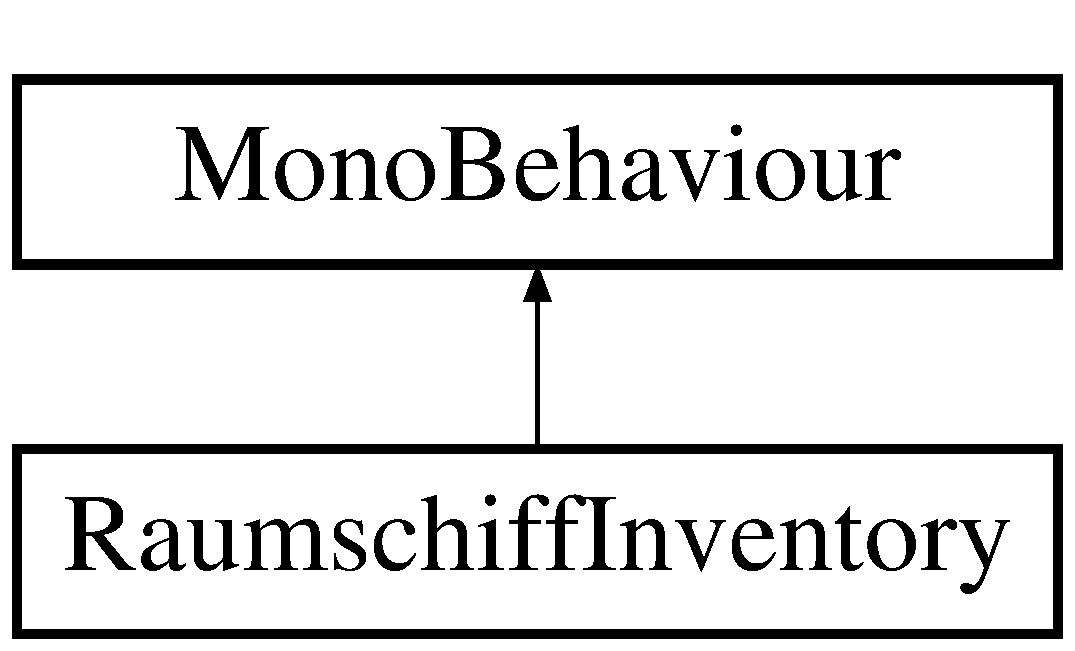
\includegraphics[height=2.000000cm]{class_raumschiff_inventory}
\end{center}
\end{figure}
\subsection*{Public Member Functions}
\begin{DoxyCompactItemize}
\item 
\mbox{\Hypertarget{class_raumschiff_inventory_afc5c732909d46de0120f565bfb46b3ee}\label{class_raumschiff_inventory_afc5c732909d46de0120f565bfb46b3ee}} 
void {\bfseries reset\+\_\+buttons} ()
\item 
\mbox{\Hypertarget{class_raumschiff_inventory_ad4afc170f452b87c3e458e698e01e78e}\label{class_raumschiff_inventory_ad4afc170f452b87c3e458e698e01e78e}} 
void {\bfseries set\+\_\+buttons} ()
\end{DoxyCompactItemize}
\subsection*{Public Attributes}
\begin{DoxyCompactItemize}
\item 
\mbox{\Hypertarget{class_raumschiff_inventory_a13419ddb20af9509fef81affd54b1d86}\label{class_raumschiff_inventory_a13419ddb20af9509fef81affd54b1d86}} 
Game\+Object {\bfseries item\+\_\+button}
\item 
\mbox{\Hypertarget{class_raumschiff_inventory_a164ab7c879ee868d2953509bbbbde5f5}\label{class_raumschiff_inventory_a164ab7c879ee868d2953509bbbbde5f5}} 
Rect\+Transform {\bfseries item\+\_\+button\+\_\+rt}
\item 
\mbox{\Hypertarget{class_raumschiff_inventory_ad35b02c4f9e4e24fcf4ec60603aff170}\label{class_raumschiff_inventory_ad35b02c4f9e4e24fcf4ec60603aff170}} 
Text {\bfseries impuls\+\_\+antrieb\+\_\+text}
\item 
\mbox{\Hypertarget{class_raumschiff_inventory_ad582bf87bd94f8876f348432918cd839}\label{class_raumschiff_inventory_ad582bf87bd94f8876f348432918cd839}} 
Text {\bfseries schild\+\_\+text}
\item 
\mbox{\Hypertarget{class_raumschiff_inventory_ab71281ffbe8f3b64f94ddde919ea85ac}\label{class_raumschiff_inventory_ab71281ffbe8f3b64f94ddde919ea85ac}} 
Text {\bfseries top\+\_\+weapon\+\_\+text}
\item 
\mbox{\Hypertarget{class_raumschiff_inventory_a8832281e3648f14fb237a8226efcc61d}\label{class_raumschiff_inventory_a8832281e3648f14fb237a8226efcc61d}} 
Text {\bfseries bot\+\_\+weapon\+\_\+text}
\item 
\mbox{\Hypertarget{class_raumschiff_inventory_a9e4927b2e083517c9c3db1db58c27870}\label{class_raumschiff_inventory_a9e4927b2e083517c9c3db1db58c27870}} 
Game\+Object {\bfseries impuls\+\_\+antrieb\+\_\+button}
\item 
\mbox{\Hypertarget{class_raumschiff_inventory_a6519212a6c5ee2492e2718f761e487bc}\label{class_raumschiff_inventory_a6519212a6c5ee2492e2718f761e487bc}} 
Game\+Object {\bfseries schild\+\_\+button}
\item 
\mbox{\Hypertarget{class_raumschiff_inventory_a3fbadb8a028bbeaf05271807b320c636}\label{class_raumschiff_inventory_a3fbadb8a028bbeaf05271807b320c636}} 
List$<$ Game\+Object $>$ {\bfseries top\+\_\+weapon\+\_\+buttons}
\item 
\mbox{\Hypertarget{class_raumschiff_inventory_ae3fc542f4d537cef97571a7b9b0eed35}\label{class_raumschiff_inventory_ae3fc542f4d537cef97571a7b9b0eed35}} 
List$<$ Game\+Object $>$ {\bfseries bot\+\_\+weapon\+\_\+buttons}
\end{DoxyCompactItemize}
\subsection*{Static Public Attributes}
\begin{DoxyCompactItemize}
\item 
\mbox{\Hypertarget{class_raumschiff_inventory_a6f027b9779464645116e2de940e81cfe}\label{class_raumschiff_inventory_a6f027b9779464645116e2de940e81cfe}} 
static \hyperlink{class_raumschiff_inventory}{Raumschiff\+Inventory} {\bfseries raumschiff\+Inventory}
\end{DoxyCompactItemize}


The documentation for this class was generated from the following file\+:\begin{DoxyCompactItemize}
\item 
/\+Users/\+Leonard/\+Desktop/\+Stor\+Trok/\+Stor Trok/\+Assets/\+Stor Trok/\+Scripts/\+U\+I/\+Inventory/Raumschiff\+Inventory.\+cs\end{DoxyCompactItemize}

\hypertarget{class_raumschiff_shop}{}\section{Raumschiff\+Shop Class Reference}
\label{class_raumschiff_shop}\index{Raumschiff\+Shop@{Raumschiff\+Shop}}
Inheritance diagram for Raumschiff\+Shop\+:\begin{figure}[H]
\begin{center}
\leavevmode
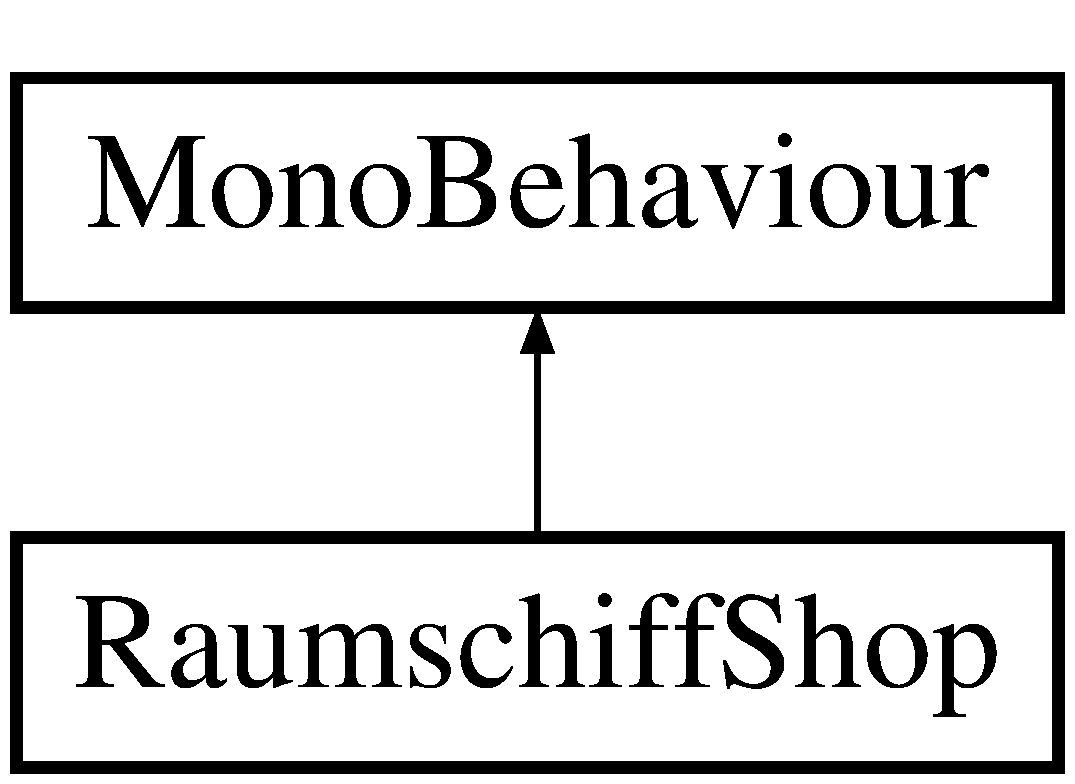
\includegraphics[height=2.000000cm]{class_raumschiff_shop}
\end{center}
\end{figure}
\subsection*{Public Attributes}
\begin{DoxyCompactItemize}
\item 
\mbox{\Hypertarget{class_raumschiff_shop_a43bed463be369cd868f8e6d68760ac0b}\label{class_raumschiff_shop_a43bed463be369cd868f8e6d68760ac0b}} 
Game\+Object {\bfseries arrow}
\item 
\mbox{\Hypertarget{class_raumschiff_shop_a83d8f2582774ec965b8f7dfc366ef4ea}\label{class_raumschiff_shop_a83d8f2582774ec965b8f7dfc366ef4ea}} 
float {\bfseries arrow\+\_\+height}
\item 
\mbox{\Hypertarget{class_raumschiff_shop_a767e001f7278dc08135c2431266c19a8}\label{class_raumschiff_shop_a767e001f7278dc08135c2431266c19a8}} 
Vector3 {\bfseries arrow\+\_\+target\+\_\+position}
\item 
\mbox{\Hypertarget{class_raumschiff_shop_a3fa42043b4688589fc47427d4d48a882}\label{class_raumschiff_shop_a3fa42043b4688589fc47427d4d48a882}} 
Game\+Object \mbox{[}$\,$\mbox{]} {\bfseries raumschiffe}
\end{DoxyCompactItemize}


The documentation for this class was generated from the following file\+:\begin{DoxyCompactItemize}
\item 
/\+Users/\+Leonard/\+Desktop/\+Stor\+Trok/\+Stor Trok/\+Assets/\+Stor Trok/\+Scripts/\+Shop/Raumschiff\+Shop.\+cs\end{DoxyCompactItemize}

\hypertarget{class_rotate_around_a_i}{}\section{Rotate\+Around\+AI Class Reference}
\label{class_rotate_around_a_i}\index{Rotate\+Around\+AI@{Rotate\+Around\+AI}}
Inheritance diagram for Rotate\+Around\+AI\+:\begin{figure}[H]
\begin{center}
\leavevmode
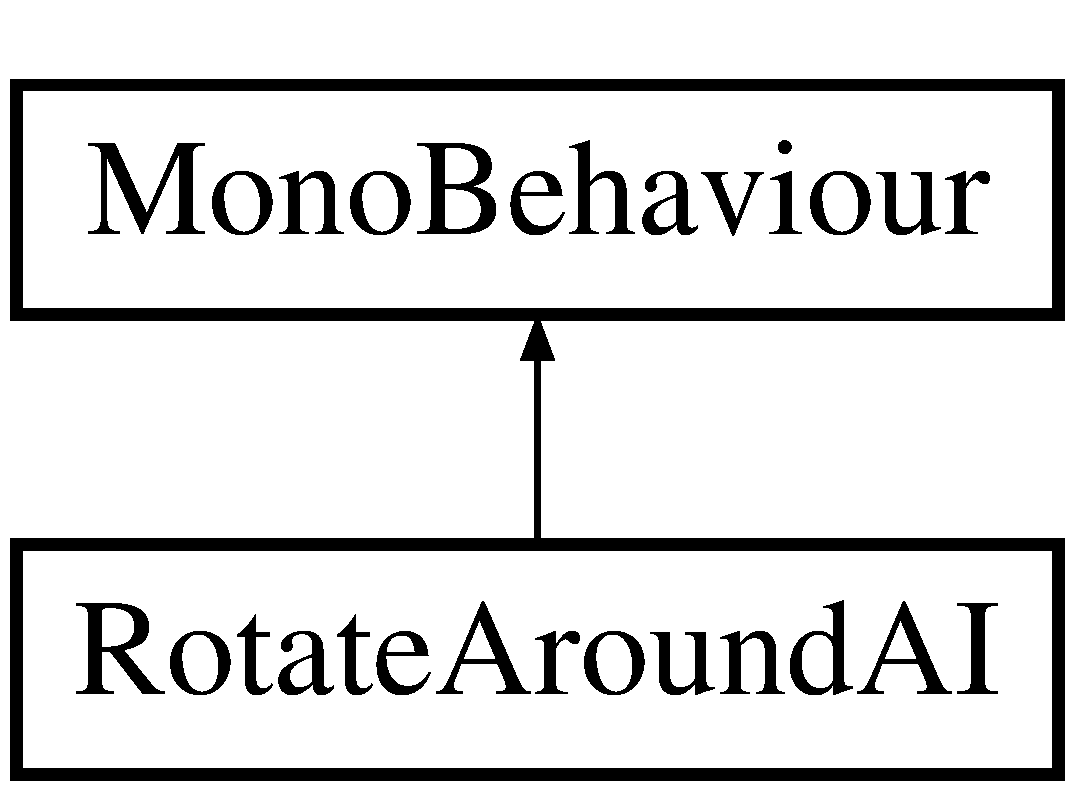
\includegraphics[height=2.000000cm]{class_rotate_around_a_i}
\end{center}
\end{figure}
\subsection*{Public Attributes}
\begin{DoxyCompactItemize}
\item 
\mbox{\Hypertarget{class_rotate_around_a_i_a2bf08a7e00a48c37ea3f03579c9922ad}\label{class_rotate_around_a_i_a2bf08a7e00a48c37ea3f03579c9922ad}} 
Game\+Object {\bfseries center}
\item 
\mbox{\Hypertarget{class_rotate_around_a_i_a581e5be68757c022ee2e0f05d81db86f}\label{class_rotate_around_a_i_a581e5be68757c022ee2e0f05d81db86f}} 
float {\bfseries velo} = 1
\end{DoxyCompactItemize}


The documentation for this class was generated from the following file\+:\begin{DoxyCompactItemize}
\item 
/\+Users/\+Leonard/\+Desktop/\+Stor\+Trok/\+Stor Trok/\+Assets/\+Stor Trok/\+Scripts/\+Tests/Rotate\+Around\+A\+I.\+cs\end{DoxyCompactItemize}

\hypertarget{class_save_data}{}\section{Save\+Data Class Reference}
\label{class_save_data}\index{Save\+Data@{Save\+Data}}
\subsection*{Static Public Member Functions}
\begin{DoxyCompactItemize}
\item 
\mbox{\Hypertarget{class_save_data_a0a16b997b1530e161f0b83aad7b05236}\label{class_save_data_a0a16b997b1530e161f0b83aad7b05236}} 
static void {\bfseries Save\+To\+File$<$ T $>$} (string path, T obj)
\item 
\mbox{\Hypertarget{class_save_data_a183ce6a6a1789b279ab6bb912207affa}\label{class_save_data_a183ce6a6a1789b279ab6bb912207affa}} 
static T {\bfseries Read\+From\+File$<$ T $>$} (string path)
\item 
\mbox{\Hypertarget{class_save_data_afd6e90835a2057e1be90023764862a26}\label{class_save_data_afd6e90835a2057e1be90023764862a26}} 
static bool {\bfseries file\+\_\+exists} (string path)
\end{DoxyCompactItemize}


The documentation for this class was generated from the following file\+:\begin{DoxyCompactItemize}
\item 
/\+Users/\+Leonard/\+Desktop/\+Stor\+Trok/\+Stor Trok/\+Assets/\+Stor Trok/\+Scripts/\+Data/Save\+Data.\+cs\end{DoxyCompactItemize}

\hypertarget{class_schild}{}\section{Schild Class Reference}
\label{class_schild}\index{Schild@{Schild}}
\subsection*{Public Member Functions}
\begin{DoxyCompactItemize}
\item 
\mbox{\Hypertarget{class_schild_a40ef8f568674cf3706e6bf6683ffaaa6}\label{class_schild_a40ef8f568674cf3706e6bf6683ffaaa6}} 
{\bfseries Schild} (float pmax\+\_\+shield\+\_\+power, Game\+Object go)
\item 
\mbox{\Hypertarget{class_schild_a5e7107bb7b35569a16e6fb45bfa7230b}\label{class_schild_a5e7107bb7b35569a16e6fb45bfa7230b}} 
\hyperlink{class_schild_part}{Schild\+Part} {\bfseries get\+\_\+best\+\_\+shield\+\_\+part} ()
\item 
\mbox{\Hypertarget{class_schild_a13b9f5d46a031c99ed3bccef5c8cf2d1}\label{class_schild_a13b9f5d46a031c99ed3bccef5c8cf2d1}} 
void {\bfseries setup\+\_\+shield\+\_\+parts} ()
\item 
\mbox{\Hypertarget{class_schild_ab889daf4cdcc877ea186e41838fbdba8}\label{class_schild_ab889daf4cdcc877ea186e41838fbdba8}} 
void {\bfseries change\+\_\+max\+\_\+power} (float pow)
\item 
\mbox{\Hypertarget{class_schild_aacef9213526f55a636e20129cff6c9ec}\label{class_schild_aacef9213526f55a636e20129cff6c9ec}} 
\hyperlink{class_schild_part}{Schild\+Part} {\bfseries get\+\_\+shield\+\_\+part} (Schild\+Part\+Types part)
\item 
\mbox{\Hypertarget{class_schild_aaa9cdd476e49e4712023945c708a2f98}\label{class_schild_aaa9cdd476e49e4712023945c708a2f98}} 
float {\bfseries get\+\_\+shield\+\_\+intensity\+\_\+at\+\_\+part} (Schild\+Part\+Types schildpart)
\item 
\mbox{\Hypertarget{class_schild_a53308fc46c6b82a05723d1acab5065ad}\label{class_schild_a53308fc46c6b82a05723d1acab5065ad}} 
Schild\+Part\+Types {\bfseries get\+\_\+schildpart\+\_\+at\+\_\+angle} (float angle)
\item 
\mbox{\Hypertarget{class_schild_ac7c947e063505ef589837985abb3757e}\label{class_schild_ac7c947e063505ef589837985abb3757e}} 
void {\bfseries apply\+\_\+dmg\+\_\+at\+\_\+shield\+\_\+part} (Schild\+Part\+Types schildpart, float dmg)
\item 
\mbox{\Hypertarget{class_schild_aecafbed64885f445ade907525947e05d}\label{class_schild_aecafbed64885f445ade907525947e05d}} 
void {\bfseries regenerate\+\_\+shield} (float regen\+\_\+amount)
\item 
\mbox{\Hypertarget{class_schild_ab1131b0d35fe75404fffa90725546c67}\label{class_schild_ab1131b0d35fe75404fffa90725546c67}} 
void {\bfseries transfer\+\_\+shield\+\_\+energy} (Schild\+Part\+Types p1, Schild\+Part\+Types p2, float amt)
\end{DoxyCompactItemize}
\subsection*{Static Public Member Functions}
\begin{DoxyCompactItemize}
\item 
\mbox{\Hypertarget{class_schild_a0e4558c57dc4265c120f8a8037acb8a7}\label{class_schild_a0e4558c57dc4265c120f8a8037acb8a7}} 
static string {\bfseries get\+Part\+Name} (Schild\+Part\+Types part)
\end{DoxyCompactItemize}
\subsection*{Public Attributes}
\begin{DoxyCompactItemize}
\item 
\hyperlink{class_schild_part}{Schild\+Part} \mbox{[}$\,$\mbox{]} {\bfseries shield\+\_\+parts}
\item 
\mbox{\Hypertarget{class_schild_a1f4825774fe941e08212dcc78f48a01a}\label{class_schild_a1f4825774fe941e08212dcc78f48a01a}} 
float {\bfseries max\+\_\+shield\+\_\+power}
\item 
\mbox{\Hypertarget{class_schild_a59ff88d7aeec08d7867cd9afe317d039}\label{class_schild_a59ff88d7aeec08d7867cd9afe317d039}} 
Game\+Object {\bfseries game\+Object}
\end{DoxyCompactItemize}
\subsection*{Static Public Attributes}
\begin{DoxyCompactItemize}
\item 
\mbox{\Hypertarget{class_schild_ae625b7f328d43a3329c0fad580efe128}\label{class_schild_ae625b7f328d43a3329c0fad580efe128}} 
static \hyperlink{class_range}{Range} {\bfseries top\+\_\+range} = new \hyperlink{class_range}{Range}(-\/45, 45)
\item 
\mbox{\Hypertarget{class_schild_a24f7eb6079dd872d9bf2491842786252}\label{class_schild_a24f7eb6079dd872d9bf2491842786252}} 
static \hyperlink{class_range}{Range} {\bfseries right\+\_\+range} = new \hyperlink{class_range}{Range}(45,135)
\item 
\mbox{\Hypertarget{class_schild_ab5ad027e113698bcb9d93b27ebac090b}\label{class_schild_ab5ad027e113698bcb9d93b27ebac090b}} 
static \hyperlink{class_range}{Range} {\bfseries bot\+\_\+range} = new \hyperlink{class_range}{Range} (135, 225)
\item 
\mbox{\Hypertarget{class_schild_a753a53a47f0c7e0abf6259514beeca3d}\label{class_schild_a753a53a47f0c7e0abf6259514beeca3d}} 
static \hyperlink{class_range}{Range} {\bfseries left\+\_\+range} = new \hyperlink{class_range}{Range} (225, 315)
\end{DoxyCompactItemize}
\subsection*{Properties}
\begin{DoxyCompactItemize}
\item 
\mbox{\Hypertarget{class_schild_a063dc74127ed6aeb9b723331208d46ac}\label{class_schild_a063dc74127ed6aeb9b723331208d46ac}} 
float {\bfseries max\+\_\+shield\+\_\+power\+\_\+per\+\_\+quarter}\hspace{0.3cm}{\ttfamily  \mbox{[}get\mbox{]}}
\end{DoxyCompactItemize}


\subsection{Member Data Documentation}
\mbox{\Hypertarget{class_schild_a17c1d5d5d3d4cb1247b9705d69529acc}\label{class_schild_a17c1d5d5d3d4cb1247b9705d69529acc}} 
\index{Schild@{Schild}!shield\+\_\+parts@{shield\+\_\+parts}}
\index{shield\+\_\+parts@{shield\+\_\+parts}!Schild@{Schild}}
\subsubsection{\texorpdfstring{shield\+\_\+parts}{shield\_parts}}
{\footnotesize\ttfamily \hyperlink{class_schild_part}{Schild\+Part} \mbox{[}$\,$\mbox{]} Schild.\+shield\+\_\+parts}

{\bfseries Initial value\+:}
\begin{DoxyCode}
= \textcolor{keyword}{new} \hyperlink{class_schild_part}{SchildPart}[]\{
        \textcolor{keyword}{new} \hyperlink{class_schild_part}{SchildPart}\{
            part = SchildPartTypes.Left,
            shield\_intensity = 0,
            angle\_range = \hyperlink{class_schild}{Schild}.left\_range
        \},
        \textcolor{keyword}{new} \hyperlink{class_schild_part}{SchildPart}\{
            part = SchildPartTypes.Right,
            shield\_intensity = 0,
            angle\_range = \hyperlink{class_schild}{Schild}.right\_range
        \},
        \textcolor{keyword}{new} \hyperlink{class_schild_part}{SchildPart}\{
            part = SchildPartTypes.Top,
            shield\_intensity = 0,
            angle\_range = \hyperlink{class_schild}{Schild}.top\_range
        \},
        \textcolor{keyword}{new} \hyperlink{class_schild_part}{SchildPart}\{
            part = SchildPartTypes.Bot,
            shield\_intensity = 0,
            angle\_range = \hyperlink{class_schild}{Schild}.bot\_range
        \}
    \}
\end{DoxyCode}


The documentation for this class was generated from the following file\+:\begin{DoxyCompactItemize}
\item 
/\+Users/\+Leonard/\+Desktop/\+Stor\+Trok/\+Stor Trok/\+Assets/\+Stor Trok/\+Scripts/\+Spaceship/Schild.\+cs\end{DoxyCompactItemize}

\hypertarget{class_schild_item}{}\section{Schild\+Item Class Reference}
\label{class_schild_item}\index{Schild\+Item@{Schild\+Item}}
Inheritance diagram for Schild\+Item\+:\begin{figure}[H]
\begin{center}
\leavevmode
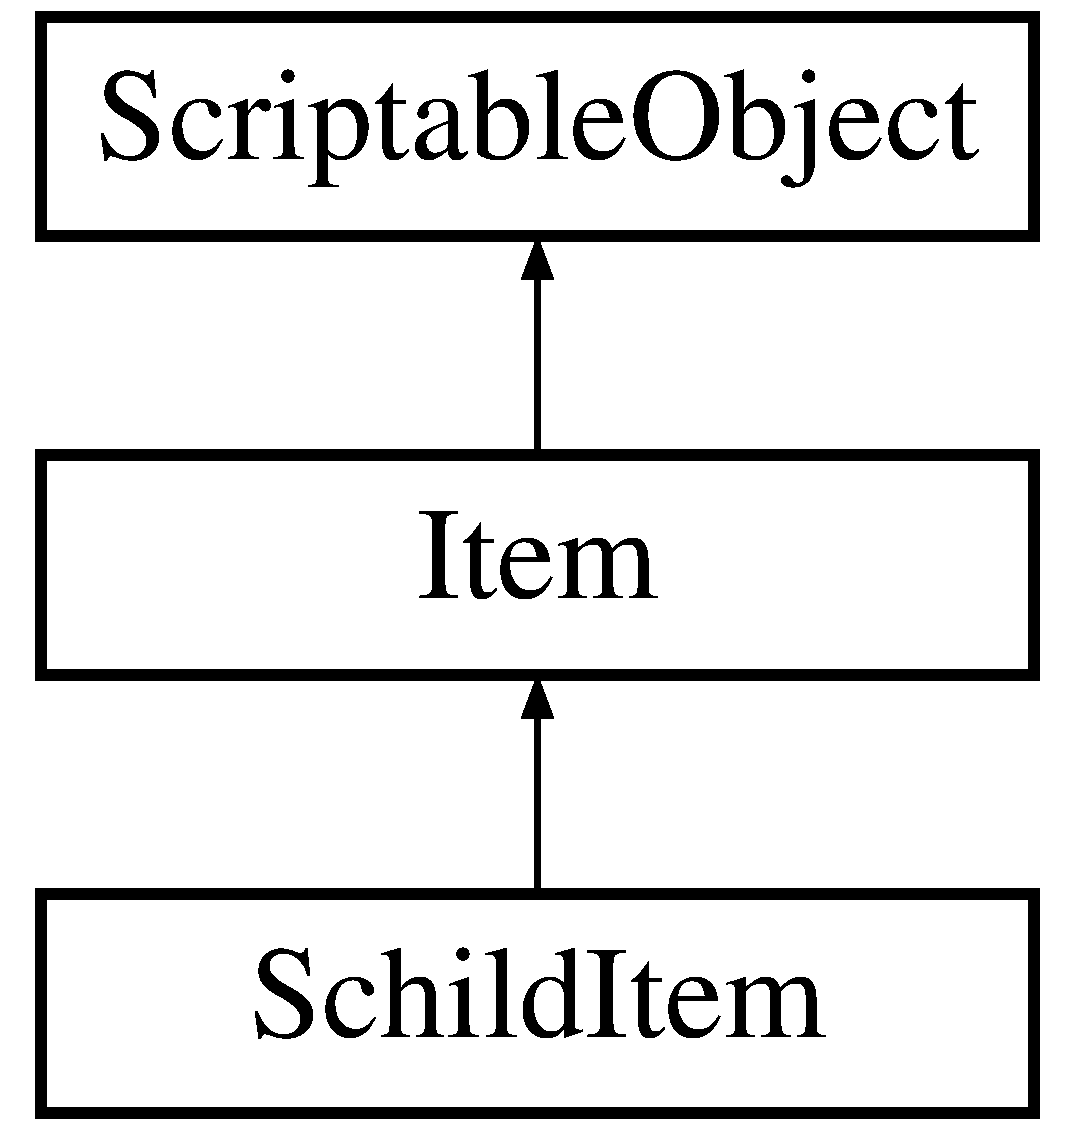
\includegraphics[height=3.000000cm]{class_schild_item}
\end{center}
\end{figure}
\subsection*{Public Member Functions}
\begin{DoxyCompactItemize}
\item 
override string \hyperlink{class_schild_item_a6e09e58ec5afc082636c1a9b4b715613}{get\+\_\+description\+\_\+text} ()
\begin{DoxyCompactList}\small\item\em Erstellt einen Text, der im \hyperlink{class_inventar}{Inventar} angezeigt wird, wenn der Mauszeiger auf dem \hyperlink{class_item}{Item} ist \end{DoxyCompactList}\end{DoxyCompactItemize}
\subsection*{Public Attributes}
\begin{DoxyCompactItemize}
\item 
\mbox{\Hypertarget{class_schild_item_a4760ae8809ff93a66903837b3826f1f0}\label{class_schild_item_a4760ae8809ff93a66903837b3826f1f0}} 
float {\bfseries max\+\_\+shield\+\_\+intenstiy}
\item 
\mbox{\Hypertarget{class_schild_item_a7d75abbdf47c1aaefe1f5590317b2976}\label{class_schild_item_a7d75abbdf47c1aaefe1f5590317b2976}} 
float {\bfseries shield\+\_\+regeneration\+\_\+rate}
\end{DoxyCompactItemize}
\subsection*{Additional Inherited Members}


\subsection{Member Function Documentation}
\mbox{\Hypertarget{class_schild_item_a6e09e58ec5afc082636c1a9b4b715613}\label{class_schild_item_a6e09e58ec5afc082636c1a9b4b715613}} 
\index{Schild\+Item@{Schild\+Item}!get\+\_\+description\+\_\+text@{get\+\_\+description\+\_\+text}}
\index{get\+\_\+description\+\_\+text@{get\+\_\+description\+\_\+text}!Schild\+Item@{Schild\+Item}}
\subsubsection{\texorpdfstring{get\+\_\+description\+\_\+text()}{get\_description\_text()}}
{\footnotesize\ttfamily override string Schild\+Item.\+get\+\_\+description\+\_\+text (\begin{DoxyParamCaption}{ }\end{DoxyParamCaption})\hspace{0.3cm}{\ttfamily [virtual]}}



Erstellt einen Text, der im \hyperlink{class_inventar}{Inventar} angezeigt wird, wenn der Mauszeiger auf dem \hyperlink{class_item}{Item} ist 

\begin{DoxyReturn}{Returns}
The description text.
\end{DoxyReturn}


Implements \hyperlink{class_item_ab868f8ccad92378f7352e3a9e0f755ff}{Item}.



The documentation for this class was generated from the following file\+:\begin{DoxyCompactItemize}
\item 
/\+Users/\+Leonard/\+Desktop/\+Stor\+Trok/\+Stor Trok/\+Assets/\+Stor Trok/\+Scripts/\+Items/Schild\+Item.\+cs\end{DoxyCompactItemize}

\hypertarget{class_schild_part}{}\section{Schild\+Part Class Reference}
\label{class_schild_part}\index{Schild\+Part@{Schild\+Part}}
\subsection*{Public Attributes}
\begin{DoxyCompactItemize}
\item 
\mbox{\Hypertarget{class_schild_part_a900286b8b48e1e2a224f9b92ebe40ab4}\label{class_schild_part_a900286b8b48e1e2a224f9b92ebe40ab4}} 
Schild\+Part\+Types {\bfseries part}
\item 
\mbox{\Hypertarget{class_schild_part_a4bd11fb17812f14e5a0b1b19c740c5bb}\label{class_schild_part_a4bd11fb17812f14e5a0b1b19c740c5bb}} 
float {\bfseries shield\+\_\+intensity}
\item 
\mbox{\Hypertarget{class_schild_part_a6986bc6860d63b4d0fc3b05c74c83709}\label{class_schild_part_a6986bc6860d63b4d0fc3b05c74c83709}} 
\hyperlink{class_range}{Range} {\bfseries angle\+\_\+range}
\end{DoxyCompactItemize}


The documentation for this class was generated from the following file\+:\begin{DoxyCompactItemize}
\item 
/\+Users/\+Leonard/\+Desktop/\+Stor\+Trok/\+Stor Trok/\+Assets/\+Stor Trok/\+Scripts/\+Spaceship/Schild.\+cs\end{DoxyCompactItemize}

\hypertarget{class_schild_shader_script}{}\section{Schild\+Shader\+Script Class Reference}
\label{class_schild_shader_script}\index{Schild\+Shader\+Script@{Schild\+Shader\+Script}}
Inheritance diagram for Schild\+Shader\+Script\+:\begin{figure}[H]
\begin{center}
\leavevmode
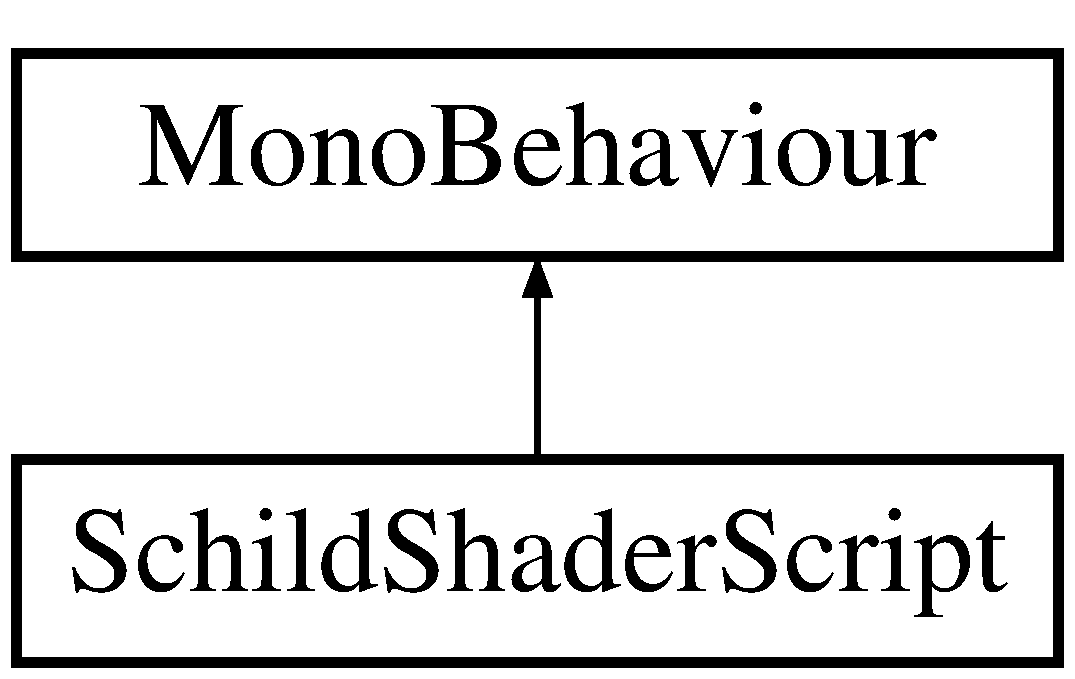
\includegraphics[height=2.000000cm]{class_schild_shader_script}
\end{center}
\end{figure}
\subsection*{Public Member Functions}
\begin{DoxyCompactItemize}
\item 
\mbox{\Hypertarget{class_schild_shader_script_ada7e33cd5e79283940406fcb0ad496ae}\label{class_schild_shader_script_ada7e33cd5e79283940406fcb0ad496ae}} 
void {\bfseries update\+\_\+colors} ()
\item 
\mbox{\Hypertarget{class_schild_shader_script_a7fbf9059b3dd81f8960929ffb991711c}\label{class_schild_shader_script_a7fbf9059b3dd81f8960929ffb991711c}} 
void {\bfseries col} (Vector3 pos)
\end{DoxyCompactItemize}
\subsection*{Public Attributes}
\begin{DoxyCompactItemize}
\item 
\mbox{\Hypertarget{class_schild_shader_script_ae129f6ef67e8cec9bdabaa4095fae180}\label{class_schild_shader_script_ae129f6ef67e8cec9bdabaa4095fae180}} 
List$<$ \hyperlink{struct_explosion_point}{Explosion\+Point} $>$ {\bfseries explosion\+\_\+points} = new List$<$\hyperlink{struct_explosion_point}{Explosion\+Point}$>$()
\item 
\mbox{\Hypertarget{class_schild_shader_script_aac6712e57dd87fe82912d5d7a8d4f3b4}\label{class_schild_shader_script_aac6712e57dd87fe82912d5d7a8d4f3b4}} 
Color {\bfseries point\+\_\+color} = new Color(0,0,1,1)
\item 
\mbox{\Hypertarget{class_schild_shader_script_a6a4af906d540b5318ac89cb946b8d099}\label{class_schild_shader_script_a6a4af906d540b5318ac89cb946b8d099}} 
Color {\bfseries normal\+\_\+color} = new Color(0.\+1f,0.\+1f,1,0.\+08f)
\item 
\mbox{\Hypertarget{class_schild_shader_script_aab156c5a7256b1a323afc8b369fe5781}\label{class_schild_shader_script_aab156c5a7256b1a323afc8b369fe5781}} 
float {\bfseries max\+\_\+explosion\+\_\+radius} = 9
\item 
\mbox{\Hypertarget{class_schild_shader_script_a55cd3a4ab58ea2de7d0fcf2bed4f5d28}\label{class_schild_shader_script_a55cd3a4ab58ea2de7d0fcf2bed4f5d28}} 
float {\bfseries explosion\+\_\+radius\+\_\+growth} = 42
\item 
\mbox{\Hypertarget{class_schild_shader_script_aeb7b40e3c59b74128faae68115083c61}\label{class_schild_shader_script_aeb7b40e3c59b74128faae68115083c61}} 
float {\bfseries start\+\_\+explosion\+\_\+radius} = 5
\end{DoxyCompactItemize}
\subsection*{Protected Attributes}
\begin{DoxyCompactItemize}
\item 
\mbox{\Hypertarget{class_schild_shader_script_a1b7e209c692fb4fefcd5a052bebb66bc}\label{class_schild_shader_script_a1b7e209c692fb4fefcd5a052bebb66bc}} 
bool {\bfseries is\+\_\+explosion} = false
\end{DoxyCompactItemize}


The documentation for this class was generated from the following file\+:\begin{DoxyCompactItemize}
\item 
/\+Users/\+Leonard/\+Desktop/\+Stor\+Trok/\+Stor Trok/\+Assets/\+Stor Trok/\+Scripts/\+Spaceship/Schild\+Shader\+Script.\+cs\end{DoxyCompactItemize}

\hypertarget{class_serializable_vector3}{}\section{Serializable\+Vector3 Class Reference}
\label{class_serializable_vector3}\index{Serializable\+Vector3@{Serializable\+Vector3}}
\subsection*{Public Member Functions}
\begin{DoxyCompactItemize}
\item 
\mbox{\Hypertarget{class_serializable_vector3_ab073e8b441ca058941b210fea754373c}\label{class_serializable_vector3_ab073e8b441ca058941b210fea754373c}} 
{\bfseries Serializable\+Vector3} (Vector3 v)
\end{DoxyCompactItemize}
\subsection*{Public Attributes}
\begin{DoxyCompactItemize}
\item 
\mbox{\Hypertarget{class_serializable_vector3_a3528822b63a9561c84907caf93017a97}\label{class_serializable_vector3_a3528822b63a9561c84907caf93017a97}} 
float {\bfseries x}
\item 
\mbox{\Hypertarget{class_serializable_vector3_ae16fc8bdcb05ef764ceb25d184e5a357}\label{class_serializable_vector3_ae16fc8bdcb05ef764ceb25d184e5a357}} 
float {\bfseries y}
\item 
\mbox{\Hypertarget{class_serializable_vector3_a711c36688d7ead70f2169053edb9223c}\label{class_serializable_vector3_a711c36688d7ead70f2169053edb9223c}} 
float {\bfseries z}
\end{DoxyCompactItemize}
\subsection*{Properties}
\begin{DoxyCompactItemize}
\item 
\mbox{\Hypertarget{class_serializable_vector3_a093752c15e617cbe59247e227993778b}\label{class_serializable_vector3_a093752c15e617cbe59247e227993778b}} 
Vector3 {\bfseries unity\+\_\+vector3}\hspace{0.3cm}{\ttfamily  \mbox{[}get\mbox{]}}
\end{DoxyCompactItemize}


The documentation for this class was generated from the following file\+:\begin{DoxyCompactItemize}
\item 
/\+Users/\+Leonard/\+Desktop/\+Stor\+Trok/\+Stor Trok/\+Assets/\+Stor Trok/\+Scripts/\+Data/Save\+Data.\+cs\end{DoxyCompactItemize}

\hypertarget{class_simple_a_i1}{}\section{Simple\+A\+I1 Class Reference}
\label{class_simple_a_i1}\index{Simple\+A\+I1@{Simple\+A\+I1}}
Inheritance diagram for Simple\+A\+I1\+:\begin{figure}[H]
\begin{center}
\leavevmode
\includegraphics[height=2.000000cm]{class_simple_a_i1}
\end{center}
\end{figure}
\subsection*{Public Attributes}
\begin{DoxyCompactItemize}
\item 
\mbox{\Hypertarget{class_simple_a_i1_a570b503a7669c992d2326b238e5cdb6c}\label{class_simple_a_i1_a570b503a7669c992d2326b238e5cdb6c}} 
bool {\bfseries do\+\_\+movement\+\_\+ai}
\end{DoxyCompactItemize}


The documentation for this class was generated from the following file\+:\begin{DoxyCompactItemize}
\item 
/\+Users/\+Leonard/\+Desktop/\+Stor\+Trok/\+Stor Trok/\+Assets/\+Stor Trok/\+Scripts/\+Computer\+Players/\+Movement\+Types/Simple\+A\+I1.\+cs\end{DoxyCompactItemize}

\hypertarget{class_spaceship}{}\section{Spaceship Class Reference}
\label{class_spaceship}\index{Spaceship@{Spaceship}}
Inheritance diagram for Spaceship\+:\begin{figure}[H]
\begin{center}
\leavevmode
\includegraphics[height=2.000000cm]{class_spaceship}
\end{center}
\end{figure}
\subsection*{Public Member Functions}
\begin{DoxyCompactItemize}
\item 
void \hyperlink{class_spaceship_a65c885ff5b2c4b2142d02ed093d734a2}{setup\+\_\+standard\+\_\+items} ()
\begin{DoxyCompactList}\small\item\em Legt die Items fest, die standardmäßig auf dem \hyperlink{class_raumschiff}{Raumschiff} vorhanden sind. (Das gilt nicht für den Spieler selbst, da dieser auch eigene Item-\/\+Kombinationen auf seinem \hyperlink{class_raumschiff}{Raumschiff} haben kann.) \end{DoxyCompactList}\item 
void \hyperlink{class_spaceship_a465e9ba15923826055b2fd43be83d635}{apply\+\_\+item\+\_\+stats} ()
\begin{DoxyCompactList}\small\item\em Setzt die Schild-\/ und Geschwindigkeitswerte den Items entsprechend fest \end{DoxyCompactList}\item 
void \hyperlink{class_spaceship_a51fd63c3c0bf5f1bb5d5d7e05db87056}{neues\+\_\+schild} (\hyperlink{class_schild_item}{Schild\+Item} schild\+\_\+neu)
\begin{DoxyCompactList}\small\item\em Neues Schild-\/\+Item für dieses \hyperlink{class_raumschiff}{Raumschiff}, z.\+B. wenn der Spieler eins aus seinem \hyperlink{class_inventar}{Inventar} in den Schild-\/\+Item-\/\+Slot zieht \end{DoxyCompactList}\item 
void \hyperlink{class_spaceship_a627ae269cfe0db00d361c9e4a8ce2413}{set\+\_\+layer} (int n\+\_\+layer)
\begin{DoxyCompactList}\small\item\em Setzt für das Object selbst und das Collision Object das Layer fest \end{DoxyCompactList}\item 
void \hyperlink{class_spaceship_a0e562e25b6f8186c569fbc0577ef3bb6}{apply\+\_\+statuseffect} (\hyperlink{class_status_effect}{Status\+Effect} ef)
\begin{DoxyCompactList}\small\item\em Fügt einen neuen \hyperlink{class_status_effect}{Status\+Effect} zu dem \hyperlink{class_raumschiff}{Raumschiff} hinzu \end{DoxyCompactList}\item 
void \hyperlink{class_spaceship_a4170fcea7d1c1cb131e634a28ad3b271}{apply\+\_\+statuseffects} (\hyperlink{class_status_effect}{Status\+Effect}\mbox{[}$\,$\mbox{]} effects)
\begin{DoxyCompactList}\small\item\em Fügt mehrere Status\+Effects hinzu \end{DoxyCompactList}\item 
void \hyperlink{class_spaceship_acc4b097a3bfdc0cbefe00246dbbcb534}{remove\+\_\+statuseffect} (\hyperlink{class_status_effect}{Status\+Effect} ef)
\begin{DoxyCompactList}\small\item\em Entfernt einen speziellen \hyperlink{class_status_effect}{Status\+Effect} \end{DoxyCompactList}\item 
void \hyperlink{class_spaceship_aa022b21fc3d102181d347b1bc1e81cba}{remove\+\_\+statuseffects} (\hyperlink{class_status_effect}{Status\+Effect}\mbox{[}$\,$\mbox{]} effects)
\begin{DoxyCompactList}\small\item\em Entfernt mehrere Status\+Effects \end{DoxyCompactList}\item 
void \hyperlink{class_spaceship_accc7fe7a6f5df4f43fa8b3ab7469c3c7}{rotation\+\_\+input} (Movement\+Input\+Keys key)
\begin{DoxyCompactList}\small\item\em Führt einen gegebenen Rotation-\/\+Input aus \end{DoxyCompactList}\item 
void \hyperlink{class_spaceship_a5c0e06422ea1860e18dce8171a585676}{speed\+\_\+input} (Movement\+Input\+Keys key)
\begin{DoxyCompactList}\small\item\em Führt einen gegebenen Speed-\/\+Input aus \end{DoxyCompactList}\item 
void \hyperlink{class_spaceship_afd788bbc8497cb88acb1c4633a3b1bb3}{fix\+\_\+rotation} ()
\begin{DoxyCompactList}\small\item\em Nur für einige \hyperlink{class_computer_player}{Computer\+Player} Da das \hyperlink{class_raumschiff}{Raumschiff} sich in lokalen-\/\+Achse maximal um einen bestimmten Winkel drehen darf und in der lokalen z-\/\+Achse gar nicht, wird hier daher die Rotation angepasst \end{DoxyCompactList}\item 
void \hyperlink{class_spaceship_ae5251fec3b08bf9b4e34e2e854e27e9f}{fix\+\_\+z\+\_\+rotation} ()
\begin{DoxyCompactList}\small\item\em Passt die lokale z-\/\+Rotation an \end{DoxyCompactList}\item 
void \hyperlink{class_spaceship_af4e61eb0614f6933afff28f8f12bbdb9}{fix\+\_\+x\+\_\+rotation} ()
\begin{DoxyCompactList}\small\item\em Passt die lokale-\/x-\/\+Rotation an \end{DoxyCompactList}\item 
void \hyperlink{class_spaceship_a0b021ca84c90939591bb5068542c1dde}{rotate\+\_\+left} ()
\begin{DoxyCompactList}\small\item\em Dreht das \hyperlink{class_raumschiff}{Raumschiff} nach links \end{DoxyCompactList}\item 
void \hyperlink{class_spaceship_adaa371fa37ba5b564b15a35b3ff94437}{rotate\+\_\+right} ()
\begin{DoxyCompactList}\small\item\em Dreht das \hyperlink{class_raumschiff}{Raumschiff} nach rechts \end{DoxyCompactList}\item 
void \hyperlink{class_spaceship_a1f8779409140a15e00f3cb4b5c7bec14}{rotate\+\_\+down} ()
\item 
void \hyperlink{class_spaceship_a311d6c40b0c54f11a2da4624a5e2487c}{rotate\+\_\+up} ()
\begin{DoxyCompactList}\small\item\em Dreht das \hyperlink{class_raumschiff}{Raumschiff} nach oben \end{DoxyCompactList}\item 
List$<$ \hyperlink{class_weapon}{Weapon} $>$ \hyperlink{class_spaceship_aa55156010da7dba1748429efda244d04}{get\+\_\+possible\+\_\+weapons} (Game\+Object enemy)
\begin{DoxyCompactList}\small\item\em Erstellt eine Liste alle Waffen auf dem \hyperlink{class_raumschiff}{Raumschiff}, die theoretisch vom Winkel her gesehen auf den Gegner schießen könnten und gibt diese zurück \end{DoxyCompactList}\item 
\hyperlink{class_spaceship_weapon_position}{Spaceship\+Weapon\+Position} \hyperlink{class_spaceship_abe7281c6b8a4d3e9294c56e6a1cf8157}{get\+\_\+top\+\_\+weapon\+\_\+position} ()
\begin{DoxyCompactList}\small\item\em Gibt die \hyperlink{class_spaceship_weapon_position}{Spaceship\+Weapon\+Position} zurück, die vorne ist und in die vordere Richtung zeigt \end{DoxyCompactList}\item 
\hyperlink{class_spaceship_weapon_position}{Spaceship\+Weapon\+Position} \hyperlink{class_spaceship_a35fbba50c658617e939fd2d82bf33fbf}{get\+\_\+bot\+\_\+weapon\+\_\+position} ()
\begin{DoxyCompactList}\small\item\em Gibt die \hyperlink{class_spaceship_weapon_position}{Spaceship\+Weapon\+Position} zurück, die hinten ist und in die hintere Richtung zeigt \end{DoxyCompactList}\item 
void \hyperlink{class_spaceship_a18e0ef162384544259aa3ec4f55ad5f8}{setup\+\_\+shield\+\_\+gos} ()
\begin{DoxyCompactList}\small\item\em Legt die Viertelkreisobjekte für den Schild-\/\+Anzeiger fest \end{DoxyCompactList}\item 
void \hyperlink{class_spaceship_a686609169faa9dec55c5da096581beec}{create\+\_\+shield} ()
\begin{DoxyCompactList}\small\item\em Erstellt eine neue Schild-\/\+Instanz für dieses \hyperlink{class_raumschiff}{Raumschiff} \end{DoxyCompactList}\item 
void \hyperlink{class_spaceship_a4a932f067ed922c34f82fa4479dbdf4d}{warp\+\_\+in} ()
\begin{DoxyCompactList}\small\item\em Lässt das \hyperlink{class_raumschiff}{Raumschiff} reinwarpen \end{DoxyCompactList}\item 
void \hyperlink{class_spaceship_a2e51bf3ac0ada83d93bb8a474994a210}{clamp\+\_\+speed} ()
\begin{DoxyCompactList}\small\item\em Grenzt den speed-\/\+Wert ein \end{DoxyCompactList}\item 
void \hyperlink{class_spaceship_a311d0678e160eb4115fcc756f4ca1bfb}{auto\+\_\+navigate\+\_\+to\+\_\+object} (Game\+Object point)
\begin{DoxyCompactList}\small\item\em Auto-\/\+Pilot zu einem Game\+Object \end{DoxyCompactList}\item 
void \hyperlink{class_spaceship_a9e01091d877ec35797334f53e1a6faa6}{auto\+\_\+navigate\+\_\+to\+\_\+object} (Game\+Object point, float target\+\_\+speed)
\begin{DoxyCompactList}\small\item\em Auto-\/\+Pilot zu einem Game\+Object mit neuer target\+\_\+speed \end{DoxyCompactList}\item 
void \hyperlink{class_spaceship_a43e9cd085c3e2cdec0122b6f4b3c6456}{auto\+\_\+navigate\+\_\+to\+\_\+point} (Vector3 point)
\begin{DoxyCompactList}\small\item\em Auto-\/\+Pilot zu einem Punkt \end{DoxyCompactList}\item 
void \hyperlink{class_spaceship_a888beaebbb837300c645eb0bc3e979e0}{abort\+\_\+auto\+\_\+navigation} ()
\begin{DoxyCompactList}\small\item\em Bricht den Auto-\/\+Piloten ab \end{DoxyCompactList}\item 
void \hyperlink{class_spaceship_ab0ef968d5442e5d536bcc0d887beacc6}{set\+\_\+target\+\_\+speed} (float s)
\begin{DoxyCompactList}\small\item\em Setzt eine Zielgeschwindigkeit für das \hyperlink{class_raumschiff}{Raumschiff} \end{DoxyCompactList}\item 
void \hyperlink{class_spaceship_a0eaf7f4995770c01eafeabe3a43c2af3}{set\+\_\+shieldpart\+\_\+color} (Game\+Object shield, Color color)
\begin{DoxyCompactList}\small\item\em Legt die Farbe für ein Viertelkreis-\/\+Schildobject fest \end{DoxyCompactList}\item 
Color \hyperlink{class_spaceship_a78e68df6007c48431f1bddf304226948}{get\+\_\+shield\+\_\+color} (float p)
\begin{DoxyCompactList}\small\item\em Berechnet die Schildfarbe für die prozentuale Schildstärke p \end{DoxyCompactList}\item 
void \hyperlink{class_spaceship_ade12946ccbbfffb92a864b710dc2217d}{set\+\_\+shield\+\_\+indicator\+\_\+color} ()
\begin{DoxyCompactList}\small\item\em Legt die Farben für die Schild-\/\+Viertelkreise fest \end{DoxyCompactList}\item 
void \hyperlink{class_spaceship_a06f201982238a71b99c5f065d48c3acc}{cloak} ()
\begin{DoxyCompactList}\small\item\em Tarnt das \hyperlink{class_raumschiff}{Raumschiff} \end{DoxyCompactList}\item 
void \hyperlink{class_spaceship_a46d165fefc78bd0cd729429b59a6bbb6}{decloak} ()
\begin{DoxyCompactList}\small\item\em Enttarnt das \hyperlink{class_raumschiff}{Raumschiff} \end{DoxyCompactList}\item 
void \hyperlink{class_spaceship_aec76ac225db6e42b52afb3aac04f7cad}{apply\+\_\+damage} (float dmg\+\_\+to\+\_\+shield, Schild\+Part\+Types schildpart, float dmg\+\_\+to\+\_\+si)
\begin{DoxyCompactList}\small\item\em Richtet Schaden am \hyperlink{class_raumschiff}{Raumschiff} an \end{DoxyCompactList}\item 
void \hyperlink{class_spaceship_a3f59582cf969851ab6633b4cf1047f20}{check\+\_\+destroyed} ()
\begin{DoxyCompactList}\small\item\em Prüft, ob das \hyperlink{class_raumschiff}{Raumschiff} zerstört werden soll und tut dies ggf. \end{DoxyCompactList}\item 
void \hyperlink{class_spaceship_a720b65b98cede503822fcb0141873f97}{destroy} ()
\begin{DoxyCompactList}\small\item\em Zerstört das \hyperlink{class_raumschiff}{Raumschiff} \end{DoxyCompactList}\item 
float \hyperlink{class_spaceship_a8cfcff835d6cba6b9fb8aa6841aa0cba}{get\+\_\+angle} (Vector3 global\+\_\+pos)
\begin{DoxyCompactList}\small\item\em Gibt den Winkel der der Punkt global\+\_\+pos auf der Raumschiff-\/\+Ebene mit dem Vorwärtsvektor bildet 0° bedeutet z.\+B. Vorne \end{DoxyCompactList}\item 
void \hyperlink{class_spaceship_abe51aab2bda242c27d475e50685bda63}{attack\+\_\+enemy} (Game\+Object enemy, int layer, Weapon\+Raw\+Types weapon\+\_\+type)
\begin{DoxyCompactList}\small\item\em Greift den Gegner an \end{DoxyCompactList}\item 
void \hyperlink{class_spaceship_a4bce8027749e4c12088266071ba6a5cc}{attack\+\_\+enemy} (Game\+Object enemy, int layer, Weapon\+Raw\+Types weapon\+\_\+type, bool recursive)
\begin{DoxyCompactList}\small\item\em Greift den Gegner an \end{DoxyCompactList}\end{DoxyCompactItemize}
\subsection*{Static Public Member Functions}
\begin{DoxyCompactItemize}
\item 
static \hyperlink{class_spaceship}{Spaceship} \hyperlink{class_spaceship_a46ebdafb571812867be422a6beb4ad21}{get\+\_\+spaceship} (Game\+Object o)
\begin{DoxyCompactList}\small\item\em Findet die Spaceship-\/\+Instanz, die auf dem Game\+Object oder in einem seiner Parents ist, oder null, wenn diese nicht existiert \end{DoxyCompactList}\item 
\mbox{\Hypertarget{class_spaceship_a57fc32dd2636651fef55762f24c8bbcf}\label{class_spaceship_a57fc32dd2636651fef55762f24c8bbcf}} 
static List$<$ \hyperlink{class_spaceship}{Spaceship} $>$ {\bfseries get\+\_\+active\+\_\+enemy\+\_\+spaceships} ()
\item 
\mbox{\Hypertarget{class_spaceship_aaffca9101612342b71a4b9b237c2df69}\label{class_spaceship_aaffca9101612342b71a4b9b237c2df69}} 
static List$<$ \hyperlink{class_spaceship}{Spaceship} $>$ {\bfseries get\+\_\+active\+\_\+player\+\_\+spaceships} ()
\end{DoxyCompactItemize}
\subsection*{Public Attributes}
\begin{DoxyCompactItemize}
\item 
\hyperlink{class_raumschiff}{Raumschiff} \hyperlink{class_spaceship_a771d4dcd411d0d08d1c2a67fd6b5f5c1}{raumschiff}
\begin{DoxyCompactList}\small\item\em Ein Scriptable\+Object mit den nötigen Informationen zu diesem \hyperlink{class_spaceship}{Spaceship} \end{DoxyCompactList}\item 
const float \hyperlink{class_spaceship_a862815bd4b04d532e2894ced48d2acc6}{min\+\_\+out\+\_\+of\+\_\+combat\+\_\+time} = 5
\begin{DoxyCompactList}\small\item\em die Zeit, in der man nicht im Kampf sein darf, um den \char`\"{}out-\/of-\/combat\char`\"{} status zu erhalten \end{DoxyCompactList}\item 
const float \hyperlink{class_spaceship_a44d9e635e6d659a4de6808bb36770ea5}{max\+\_\+x\+\_\+rotation} = 65
\begin{DoxyCompactList}\small\item\em Gibt den maximalen Drehwinkel an, den ein nicht-\/\+Spieler-\/\+Raumschiff in der lokalen x-\/\+Achse haben kann \end{DoxyCompactList}\item 
Object\+Group\+Type \hyperlink{class_spaceship_a3b6cdeee7ecba55cf3807661e8662bea}{spaceship\+\_\+group\+\_\+type} = Object\+Group\+Type.\+None
\begin{DoxyCompactList}\small\item\em Die Gruppe, in der diese Spaceship-\/\+Instanz drin ist (Spieler/\+Gegner) \end{DoxyCompactList}\item 
bool \hyperlink{class_spaceship_acdd2d51050e8368133ae24362d7b2ddf}{spaceship\+\_\+stats\+\_\+depend\+\_\+on\+\_\+items} = true
\begin{DoxyCompactList}\small\item\em Gibt an, ob die \hyperlink{class_spaceship}{Spaceship} stats (Geschwindigkeit etc.) von den Items abhängen und nicht von den Werten, die im Inspector zugeordnet wurden. ( Wurde früher für Test-\/\+Zwecke benutzt, jetzt aber nicht mehr. \end{DoxyCompactList}\item 
\hyperlink{class_schild}{Schild} \hyperlink{class_spaceship_a45e154e6dacd6da7c800c94a05dd27b0}{schild}
\begin{DoxyCompactList}\small\item\em Eine Schild-\/\+Instanz, die die Informationen bezüglich Schildstärke etc. beinhaltet. \end{DoxyCompactList}\item 
Game\+Object \hyperlink{class_spaceship_acef63fb7a63f7ee3cd351ecbbaaf4347}{warp\+\_\+in\+\_\+startpoint}
\begin{DoxyCompactList}\small\item\em Wenn das \hyperlink{class_raumschiff}{Raumschiff} am Anfang in die Szene reinwarpen sollte, gibt dieses Game\+Object die Position des Punktes an, an dem der Warpflug beginnt \end{DoxyCompactList}\item 
Game\+Object \hyperlink{class_spaceship_afe502a70397991dae3950bc9f96d9278}{warpspur}
\begin{DoxyCompactList}\small\item\em G\+FX hinter dem \hyperlink{class_raumschiff}{Raumschiff} bei Warp (wird nicht mehr benutzt) \end{DoxyCompactList}\item 
Game\+Object \hyperlink{class_spaceship_a904d291eba352540e2531359789a182f}{auspuff}
\begin{DoxyCompactList}\small\item\em G\+FX für die Impulsantriebspur \end{DoxyCompactList}\item 
float \hyperlink{class_spaceship_ae434c25796c8b4522fcb41e3abda56d9}{destroyed\+\_\+deform\+\_\+factor} = 1
\begin{DoxyCompactList}\small\item\em Bestimmt, wie stark das \hyperlink{class_spaceship}{Spaceship} bei Zerstörung verformt wird \end{DoxyCompactList}\item 
bool \hyperlink{class_spaceship_a5d9e0a694b1e357eef2f13755e8d2db1}{destroyed} = false
\begin{DoxyCompactList}\small\item\em Gibt an, ob das \hyperlink{class_raumschiff}{Raumschiff} zerstört ist. \end{DoxyCompactList}\item 
List$<$ \hyperlink{class_status_effect}{Status\+Effect} $>$ \hyperlink{class_spaceship_a54d20dc0f35e14abec24c50e060353b8}{status\+\_\+effects}
\begin{DoxyCompactList}\small\item\em Die Status-\/\+Effekte, die auf dem Schiff sind. (Buffs/\+Debuffs) \end{DoxyCompactList}\item 
bool \hyperlink{class_spaceship_a6a17ebe141b503299caf808301bf60aa}{immortal} = false
\begin{DoxyCompactList}\small\item\em Gibt an, ob das \hyperlink{class_raumschiff}{Raumschiff} zerstörbar ist. (Nur für Testzwecke) \end{DoxyCompactList}\item 
float \hyperlink{class_spaceship_a2ecf9e8c9ba5fbc7b53f731b8c364e20}{max\+\_\+structural\+\_\+integrity} = 100
\begin{DoxyCompactList}\small\item\em Die maximale Hüllenstärke \end{DoxyCompactList}\item 
float \hyperlink{class_spaceship_a7ac37ce79a081b8bc4cdedf741be9043}{structural\+\_\+integrity} = 0
\begin{DoxyCompactList}\small\item\em Die aktuelle Hüllenstärke \end{DoxyCompactList}\item 
float \hyperlink{class_spaceship_a96369ccf86f31837d7d7ae63636e780f}{max\+\_\+total\+\_\+shields} = 0
\begin{DoxyCompactList}\small\item\em Maximale Schildstärke \end{DoxyCompactList}\item 
bool \hyperlink{class_spaceship_ab3545f7f8a0bc4e106c58ee829a8c195}{minimap\+\_\+icon\+\_\+created} = false
\begin{DoxyCompactList}\small\item\em Gibt an, ob für dieses \hyperlink{class_spaceship}{Spaceship} schon ein Icon auf der \hyperlink{class_minimap}{Minimap} erstellt wurde \end{DoxyCompactList}\item 
float \hyperlink{class_spaceship_a66af2928c7df3d1050d5a730a179b922}{speed}
\begin{DoxyCompactList}\small\item\em Eingestellte Geschwindigkeit des Raumschiffs, z.\+B durch den Spieler-\/\+Input (E/Q), zwischen -\/1 und 4 \end{DoxyCompactList}\item 
float \hyperlink{class_spaceship_a28d8649c7000f2f6626f88663b4248be}{accel}
\begin{DoxyCompactList}\small\item\em Gibt an, wie stark das \hyperlink{class_raumschiff}{Raumschiff} beschleunigen kann \end{DoxyCompactList}\item 
float \hyperlink{class_spaceship_a8c2becac0f8d20fcb380a1e79b196131}{base\+\_\+rotation\+\_\+speed}
\begin{DoxyCompactList}\small\item\em Basis Drehgeschwindigkeit \end{DoxyCompactList}\item 
const float \hyperlink{class_spaceship_a1322e387e2296dbc3b47323f095d98fa}{rotation\+\_\+z\+\_\+axis\+\_\+tilt\+\_\+amount} = 20
\begin{DoxyCompactList}\small\item\em Gibt an, wie stark sich das \hyperlink{class_raumschiff}{Raumschiff} bei Links/\+Rechts-\/\+Drehung um die lokale z-\/\+Achse (vorwärts-\/\+Achse) dreht \end{DoxyCompactList}\item 
List$<$ \hyperlink{class_spaceship_weapon_position}{Spaceship\+Weapon\+Position} $>$ \hyperlink{class_spaceship_a3da1d2ff9be863bb80ea7fa2a6c3db06}{spaceship\+Weapon\+Positions}
\begin{DoxyCompactList}\small\item\em Die Waffenpositionen des Raumschiffs, also die Orte, von denen \hyperlink{class_phaser}{Phaser}, Torpedos etc. abgefeuert werden können \end{DoxyCompactList}\item 
\hyperlink{class_impuls_antrieb}{Impuls\+Antrieb} \hyperlink{class_spaceship_a2f4055a6f9d52ba2ec599e86280f5325}{impuls\+\_\+antrieb}
\begin{DoxyCompactList}\small\item\em Das Impuls-\/\+Antriebs-\/\+Item, das dem Schiff zugewiesen ist \end{DoxyCompactList}\item 
\hyperlink{class_warp_antrieb}{Warp\+Antrieb} \hyperlink{class_spaceship_a79ee5cdccdede956de6eae9a1619ccbc}{warp\+\_\+antrieb}
\begin{DoxyCompactList}\small\item\em Das Warp-\/\+Antriebs-\/\+Item, das dem Schiff zugewiesen ist \end{DoxyCompactList}\item 
Antrieb\+Type \hyperlink{class_spaceship_ad33632d0f3e88bdeae6f711044e53a4e}{antrieb\+\_\+type} = Antrieb\+Type.\+Impuls
\begin{DoxyCompactList}\small\item\em Der Antrieb, der zurzeit benutzt wird (Warp/\+Impuls) \end{DoxyCompactList}\item 
List$<$ \hyperlink{class_spaceship_module}{Spaceship\+Module} $>$ \hyperlink{class_spaceship_aad3c0baa850f85ef7432c0ea6f0e003e}{modules} = new List$<$\hyperlink{class_spaceship_module}{Spaceship\+Module}$>$()
\begin{DoxyCompactList}\small\item\em Die Raumschiffe-\/\+Module, mit denen dieses \hyperlink{class_raumschiff}{Raumschiff} ausgestattet ist \end{DoxyCompactList}\item 
const float \hyperlink{class_spaceship_a7a1ae8f60dc0535577c90ac06e5c86cd}{cloak\+\_\+effect\+\_\+alpha} = 0.\+4f
\begin{DoxyCompactList}\small\item\em Durchsichtigkeit des Raumschiffs bei Tarnung \end{DoxyCompactList}\item 
bool \hyperlink{class_spaceship_a012d6f0509e4e4c6afbeaa81b80c4b23}{is\+\_\+cloaking} = false
\begin{DoxyCompactList}\small\item\em Gibt an, ob sich das \hyperlink{class_raumschiff}{Raumschiff} gerade tarnt \end{DoxyCompactList}\item 
Game\+Object \hyperlink{class_spaceship_a40f7992de603fb76e22c3dcce1b63292}{schild\+\_\+collision\+\_\+object}
\begin{DoxyCompactList}\small\item\em Das Game\+Object, das für die Schild-\/\+Schild-\/\+Graphik und die Collision zuständig ist \end{DoxyCompactList}\item 
Game\+Object \hyperlink{class_spaceship_aa88ea0cfef593a18db011de1ca41c335}{gfx\+\_\+parent}
\begin{DoxyCompactList}\small\item\em Das Game\+Object, das die G\+FX beinhaltet (häufig das Object selbst) \end{DoxyCompactList}\item 
Game\+Object \hyperlink{class_spaceship_a128777395236ab7a2ef22f1f44ef903b}{shields}
\begin{DoxyCompactList}\small\item\em Die vier Game\+Objects der Viertelkreise, die die jeweilige Schildstärke angeben \end{DoxyCompactList}\item 
bool \hyperlink{class_spaceship_afe9aabc5e72224e51baf21791e026bd0}{has\+\_\+shield\+\_\+indicator} = true
\begin{DoxyCompactList}\small\item\em Gibt an, ob das \hyperlink{class_raumschiff}{Raumschiff} Schild-\/\+Anzeiger hat (die vier Viertelkreise) \end{DoxyCompactList}\item 
bool \hyperlink{class_spaceship_a17928c1e3b04001aaf33e9083731c647}{warping\+\_\+in} = false
\begin{DoxyCompactList}\small\item\em Gibt an, ob das \hyperlink{class_raumschiff}{Raumschiff} gerade am Reinwarpen ist \end{DoxyCompactList}\item 
Vector3 \hyperlink{class_spaceship_a55f3116d23628f01925dd1b7f4a053e9}{start\+\_\+pos}
\begin{DoxyCompactList}\small\item\em Startposition vor dem Reinwarpen, also Ziel des Warps \end{DoxyCompactList}\item 
Vector3 \hyperlink{class_spaceship_a1cb2c76d5ed1db05cba652b7a9cd71ca}{warpin\+\_\+start\+\_\+pos}
\begin{DoxyCompactList}\small\item\em Startposition des Reinwarpens \end{DoxyCompactList}\item 
bool \hyperlink{class_spaceship_a6088ab385c31a4133eb7418bc79dd31b}{is\+\_\+auto\+\_\+navigating}
\begin{DoxyCompactList}\small\item\em Gibt an, ob das \hyperlink{class_raumschiff}{Raumschiff} gerade den Auto-\/\+Pilot an hat \end{DoxyCompactList}\item 
Game\+Object \hyperlink{class_spaceship_ad7b81478ac9e68d3b28d84ccda1b0e5f}{auto\+\_\+navigation\+\_\+target\+\_\+object}
\begin{DoxyCompactList}\small\item\em Zielobjekt des Auto-\/\+Piloten \end{DoxyCompactList}\item 
const float \hyperlink{class_spaceship_a14d21edf96d6a77e14d975b506275e7e}{auto\+\_\+navigation\+\_\+target\+\_\+distance} = 60
\begin{DoxyCompactList}\small\item\em Gibt an, wie nah das \hyperlink{class_raumschiff}{Raumschiff} am Ziel dran sein muss, um den Auto-\/\+Piloten abzuschalten \end{DoxyCompactList}\item 
float \hyperlink{class_spaceship_a6190772ff13072113beda25fcc6469ce}{auto\+\_\+navigation\+\_\+target\+\_\+speed} = 4
\begin{DoxyCompactList}\small\item\em Normale Reisegeschwindigkeit des Auto-\/\+Piloten \end{DoxyCompactList}\item 
Vector3 \hyperlink{class_spaceship_ac19d442ae4d44180f76a3875ec0a496b}{auto\+\_\+navigation\+\_\+bug\+\_\+180\+\_\+correction\+\_\+axis} = new Vector3 (0, 1, 0)
\begin{DoxyCompactList}\small\item\em Sollte das \hyperlink{class_raumschiff}{Raumschiff} in die entgegengesetzte Richtung fliegen, muss eine neue Achse für die Rotation hinzugefügt werden. Aufgrund der Behebung eines anderen Fehlers tritt dies nun aber nicht mehr ein. (Genaugenommen ist dies kein Bug, sondern nur eine logische Konzequenz des Kreuzproduktes. Da dies aber zuerst wie ein Bug aussah, heißt es immer noch Bug) \end{DoxyCompactList}\end{DoxyCompactItemize}
\subsection*{Static Public Attributes}
\begin{DoxyCompactItemize}
\item 
static List$<$ \hyperlink{class_spaceship}{Spaceship} $>$ \hyperlink{class_spaceship_a5958b60df7a824952944bfa3c201676f}{active\+\_\+spaceships} = new List$<$\hyperlink{class_spaceship}{Spaceship}$>$ ()
\begin{DoxyCompactList}\small\item\em Alle aktiven Spaceship-\/\+Instanzen in der Scene, die nicht destroyed sind \end{DoxyCompactList}\item 
static float \hyperlink{class_spaceship_a1e950732e18a6aa13fbbc4b24bce7fe6}{max\+\_\+attack\+\_\+distance} = 2000
\begin{DoxyCompactList}\small\item\em Maximale Angriffsdistanz der Raumschiffe \end{DoxyCompactList}\end{DoxyCompactItemize}
\subsection*{Properties}
\begin{DoxyCompactItemize}
\item 
\mbox{\Hypertarget{class_spaceship_ae00fee3dd4ed5e2dc8c8c5f96505a5a3}\label{class_spaceship_ae00fee3dd4ed5e2dc8c8c5f96505a5a3}} 
\hyperlink{class_schild_item}{Schild\+Item} {\bfseries schild\+\_\+item}\hspace{0.3cm}{\ttfamily  \mbox{[}get, set\mbox{]}}
\item 
List$<$ \hyperlink{class_item}{Item} $>$ \hyperlink{class_spaceship_a89158e2a2dc71a98acb3c3755962c144}{equipped\+\_\+items}\hspace{0.3cm}{\ttfamily  \mbox{[}get\mbox{]}}
\begin{DoxyCompactList}\small\item\em Gibt eine Liste aller Items zurück, die zurzeit auf dem \hyperlink{class_raumschiff}{Raumschiff} sind \end{DoxyCompactList}\item 
float \hyperlink{class_spaceship_a9dfc7adf86ae18216d0244326e7a6ebf}{max\+\_\+speed}\hspace{0.3cm}{\ttfamily  \mbox{[}get\mbox{]}}
\begin{DoxyCompactList}\small\item\em Gibt die maximal erreichbare Geschwindigkeit zurück. Diese ist abhängig von der Basis-\/\+Geschwindigkeit, die durch das Impuls-\/\+Antrieb-\/\+Item festgelegt ist, und den Statuseffekten (Buffs/\+Debuffs), die auf dem \hyperlink{class_raumschiff}{Raumschiff} sind \end{DoxyCompactList}\item 
float \hyperlink{class_spaceship_a9dede788e870c34a09db8d22e9ac61f6}{rotation\+\_\+speed}\hspace{0.3cm}{\ttfamily  \mbox{[}get\mbox{]}}
\begin{DoxyCompactList}\small\item\em Gibt die maximal erreichbare Drehgeschwindigkeit zurück. Diese ist abhängig von der Basis-\/\+Dreheschwindigkeit und den Statuseffekten (Buffs/\+Debuffs), die auf dem \hyperlink{class_raumschiff}{Raumschiff} sind \end{DoxyCompactList}\item 
float \hyperlink{class_spaceship_ad98db7a91256b60c912c508cff2f001d}{damage\+\_\+output}\hspace{0.3cm}{\ttfamily  \mbox{[}get\mbox{]}}
\begin{DoxyCompactList}\small\item\em Gibt einen Schadens-\/\+Multiplier zurück Dieser ist abhängig von den Statuseffekten (Buffs/\+Debuffs), die auf dem \hyperlink{class_raumschiff}{Raumschiff} sind \end{DoxyCompactList}\item 
float \hyperlink{class_spaceship_a1daf5f7456d1b35b59eb6580b4ad5b9e}{shield\+\_\+modifier}\hspace{0.3cm}{\ttfamily  \mbox{[}get\mbox{]}}
\begin{DoxyCompactList}\small\item\em Gibt einen Schild-\/\+Multiplier zurück Dieser ist abhängig von den Statuseffekten (Buffs/\+Debuffs), die auf dem \hyperlink{class_raumschiff}{Raumschiff} sind \end{DoxyCompactList}\item 
bool \hyperlink{class_spaceship_a459b3d62a7e0a7e76b7a019de5b386e1}{can\+\_\+attack}\hspace{0.3cm}{\ttfamily  \mbox{[}get\mbox{]}}
\begin{DoxyCompactList}\small\item\em Prüft, ob dieses \hyperlink{class_spaceship}{Spaceship} angreifen kann. \end{DoxyCompactList}\item 
bool \hyperlink{class_spaceship_ae627cd6b28077cea3ca7d50e1c3eea8d}{ship\+\_\+under\+\_\+attack}\hspace{0.3cm}{\ttfamily  \mbox{[}get\mbox{]}}
\begin{DoxyCompactList}\small\item\em Gibt an, ob das \hyperlink{class_spaceship}{Spaceship} unter Beschuss ist \end{DoxyCompactList}\item 
bool \hyperlink{class_spaceship_a008e4fcc8af1c4ebbaee64603593d6d1}{in\+\_\+battle}\hspace{0.3cm}{\ttfamily  \mbox{[}get\mbox{]}}
\begin{DoxyCompactList}\small\item\em Gibt an, ob das \hyperlink{class_spaceship}{Spaceship} im Kampf ist. \end{DoxyCompactList}\end{DoxyCompactItemize}


\subsection{Member Function Documentation}
\mbox{\Hypertarget{class_spaceship_a888beaebbb837300c645eb0bc3e979e0}\label{class_spaceship_a888beaebbb837300c645eb0bc3e979e0}} 
\index{Spaceship@{Spaceship}!abort\+\_\+auto\+\_\+navigation@{abort\+\_\+auto\+\_\+navigation}}
\index{abort\+\_\+auto\+\_\+navigation@{abort\+\_\+auto\+\_\+navigation}!Spaceship@{Spaceship}}
\subsubsection{\texorpdfstring{abort\+\_\+auto\+\_\+navigation()}{abort\_auto\_navigation()}}
{\footnotesize\ttfamily void Spaceship.\+abort\+\_\+auto\+\_\+navigation (\begin{DoxyParamCaption}{ }\end{DoxyParamCaption})}



Bricht den Auto-\/\+Piloten ab 

\mbox{\Hypertarget{class_spaceship_aec76ac225db6e42b52afb3aac04f7cad}\label{class_spaceship_aec76ac225db6e42b52afb3aac04f7cad}} 
\index{Spaceship@{Spaceship}!apply\+\_\+damage@{apply\+\_\+damage}}
\index{apply\+\_\+damage@{apply\+\_\+damage}!Spaceship@{Spaceship}}
\subsubsection{\texorpdfstring{apply\+\_\+damage()}{apply\_damage()}}
{\footnotesize\ttfamily void Spaceship.\+apply\+\_\+damage (\begin{DoxyParamCaption}\item[{float}]{dmg\+\_\+to\+\_\+shield,  }\item[{Schild\+Part\+Types}]{schildpart,  }\item[{float}]{dmg\+\_\+to\+\_\+si }\end{DoxyParamCaption})}



Richtet Schaden am \hyperlink{class_raumschiff}{Raumschiff} an 


\begin{DoxyParams}{Parameters}
{\em dmg\+\_\+to\+\_\+shield} & Der Schaden, der dem \hyperlink{class_schild}{Schild} hinzugefügt wird.\\
\hline
{\em schildpart} & Der zu beschädigende Schildpart.\\
\hline
{\em dmg\+\_\+to\+\_\+si} & Der Schaden, der der Hülle hinzugefügt wird.\\
\hline
\end{DoxyParams}
\mbox{\Hypertarget{class_spaceship_a465e9ba15923826055b2fd43be83d635}\label{class_spaceship_a465e9ba15923826055b2fd43be83d635}} 
\index{Spaceship@{Spaceship}!apply\+\_\+item\+\_\+stats@{apply\+\_\+item\+\_\+stats}}
\index{apply\+\_\+item\+\_\+stats@{apply\+\_\+item\+\_\+stats}!Spaceship@{Spaceship}}
\subsubsection{\texorpdfstring{apply\+\_\+item\+\_\+stats()}{apply\_item\_stats()}}
{\footnotesize\ttfamily void Spaceship.\+apply\+\_\+item\+\_\+stats (\begin{DoxyParamCaption}{ }\end{DoxyParamCaption})}



Setzt die Schild-\/ und Geschwindigkeitswerte den Items entsprechend fest 

\mbox{\Hypertarget{class_spaceship_a0e562e25b6f8186c569fbc0577ef3bb6}\label{class_spaceship_a0e562e25b6f8186c569fbc0577ef3bb6}} 
\index{Spaceship@{Spaceship}!apply\+\_\+statuseffect@{apply\+\_\+statuseffect}}
\index{apply\+\_\+statuseffect@{apply\+\_\+statuseffect}!Spaceship@{Spaceship}}
\subsubsection{\texorpdfstring{apply\+\_\+statuseffect()}{apply\_statuseffect()}}
{\footnotesize\ttfamily void Spaceship.\+apply\+\_\+statuseffect (\begin{DoxyParamCaption}\item[{\hyperlink{class_status_effect}{Status\+Effect}}]{ef }\end{DoxyParamCaption})}



Fügt einen neuen \hyperlink{class_status_effect}{Status\+Effect} zu dem \hyperlink{class_raumschiff}{Raumschiff} hinzu 


\begin{DoxyParams}{Parameters}
{\em ef} & Der \hyperlink{class_status_effect}{Status\+Effect}.\\
\hline
\end{DoxyParams}
\mbox{\Hypertarget{class_spaceship_a4170fcea7d1c1cb131e634a28ad3b271}\label{class_spaceship_a4170fcea7d1c1cb131e634a28ad3b271}} 
\index{Spaceship@{Spaceship}!apply\+\_\+statuseffects@{apply\+\_\+statuseffects}}
\index{apply\+\_\+statuseffects@{apply\+\_\+statuseffects}!Spaceship@{Spaceship}}
\subsubsection{\texorpdfstring{apply\+\_\+statuseffects()}{apply\_statuseffects()}}
{\footnotesize\ttfamily void Spaceship.\+apply\+\_\+statuseffects (\begin{DoxyParamCaption}\item[{\hyperlink{class_status_effect}{Status\+Effect} \mbox{[}$\,$\mbox{]}}]{effects }\end{DoxyParamCaption})}



Fügt mehrere Status\+Effects hinzu 


\begin{DoxyParams}{Parameters}
{\em effects} & Die Status\+Effects.\\
\hline
\end{DoxyParams}
\mbox{\Hypertarget{class_spaceship_abe51aab2bda242c27d475e50685bda63}\label{class_spaceship_abe51aab2bda242c27d475e50685bda63}} 
\index{Spaceship@{Spaceship}!attack\+\_\+enemy@{attack\+\_\+enemy}}
\index{attack\+\_\+enemy@{attack\+\_\+enemy}!Spaceship@{Spaceship}}
\subsubsection{\texorpdfstring{attack\+\_\+enemy()}{attack\_enemy()}\hspace{0.1cm}{\footnotesize\ttfamily [1/2]}}
{\footnotesize\ttfamily void Spaceship.\+attack\+\_\+enemy (\begin{DoxyParamCaption}\item[{Game\+Object}]{enemy,  }\item[{int}]{layer,  }\item[{Weapon\+Raw\+Types}]{weapon\+\_\+type }\end{DoxyParamCaption})}



Greift den Gegner an 


\begin{DoxyParams}{Parameters}
{\em enemy} & Enemy.\\
\hline
{\em layer} & Layer.\\
\hline
{\em weapon\+\_\+type} & \hyperlink{class_weapon}{Weapon} type.\\
\hline
\end{DoxyParams}
\mbox{\Hypertarget{class_spaceship_a4bce8027749e4c12088266071ba6a5cc}\label{class_spaceship_a4bce8027749e4c12088266071ba6a5cc}} 
\index{Spaceship@{Spaceship}!attack\+\_\+enemy@{attack\+\_\+enemy}}
\index{attack\+\_\+enemy@{attack\+\_\+enemy}!Spaceship@{Spaceship}}
\subsubsection{\texorpdfstring{attack\+\_\+enemy()}{attack\_enemy()}\hspace{0.1cm}{\footnotesize\ttfamily [2/2]}}
{\footnotesize\ttfamily void Spaceship.\+attack\+\_\+enemy (\begin{DoxyParamCaption}\item[{Game\+Object}]{enemy,  }\item[{int}]{layer,  }\item[{Weapon\+Raw\+Types}]{weapon\+\_\+type,  }\item[{bool}]{recursive }\end{DoxyParamCaption})}



Greift den Gegner an 


\begin{DoxyParams}{Parameters}
{\em enemy} & Enemy.\\
\hline
{\em layer} & Layer.\\
\hline
{\em weapon\+\_\+type} & \hyperlink{class_weapon}{Weapon} type.\\
\hline
{\em recursive} & Gibt an, ob die selbe Waffe auf ein anderes Schiff feuern kann, wennn das ausgewählte Schiff nicht durch diese Waffe angegriffen werden kann. (Zurzeit nicht aktiv)\\
\hline
\end{DoxyParams}
\mbox{\Hypertarget{class_spaceship_a311d0678e160eb4115fcc756f4ca1bfb}\label{class_spaceship_a311d0678e160eb4115fcc756f4ca1bfb}} 
\index{Spaceship@{Spaceship}!auto\+\_\+navigate\+\_\+to\+\_\+object@{auto\+\_\+navigate\+\_\+to\+\_\+object}}
\index{auto\+\_\+navigate\+\_\+to\+\_\+object@{auto\+\_\+navigate\+\_\+to\+\_\+object}!Spaceship@{Spaceship}}
\subsubsection{\texorpdfstring{auto\+\_\+navigate\+\_\+to\+\_\+object()}{auto\_navigate\_to\_object()}\hspace{0.1cm}{\footnotesize\ttfamily [1/2]}}
{\footnotesize\ttfamily void Spaceship.\+auto\+\_\+navigate\+\_\+to\+\_\+object (\begin{DoxyParamCaption}\item[{Game\+Object}]{point }\end{DoxyParamCaption})}



Auto-\/\+Pilot zu einem Game\+Object 


\begin{DoxyParams}{Parameters}
{\em point} & Zielobjekt.\\
\hline
\end{DoxyParams}
\mbox{\Hypertarget{class_spaceship_a9e01091d877ec35797334f53e1a6faa6}\label{class_spaceship_a9e01091d877ec35797334f53e1a6faa6}} 
\index{Spaceship@{Spaceship}!auto\+\_\+navigate\+\_\+to\+\_\+object@{auto\+\_\+navigate\+\_\+to\+\_\+object}}
\index{auto\+\_\+navigate\+\_\+to\+\_\+object@{auto\+\_\+navigate\+\_\+to\+\_\+object}!Spaceship@{Spaceship}}
\subsubsection{\texorpdfstring{auto\+\_\+navigate\+\_\+to\+\_\+object()}{auto\_navigate\_to\_object()}\hspace{0.1cm}{\footnotesize\ttfamily [2/2]}}
{\footnotesize\ttfamily void Spaceship.\+auto\+\_\+navigate\+\_\+to\+\_\+object (\begin{DoxyParamCaption}\item[{Game\+Object}]{point,  }\item[{float}]{target\+\_\+speed }\end{DoxyParamCaption})}



Auto-\/\+Pilot zu einem Game\+Object mit neuer target\+\_\+speed 


\begin{DoxyParams}{Parameters}
{\em point} & Zielobjekt.\\
\hline
{\em target\+\_\+speed} & Target speed.\\
\hline
\end{DoxyParams}
\mbox{\Hypertarget{class_spaceship_a43e9cd085c3e2cdec0122b6f4b3c6456}\label{class_spaceship_a43e9cd085c3e2cdec0122b6f4b3c6456}} 
\index{Spaceship@{Spaceship}!auto\+\_\+navigate\+\_\+to\+\_\+point@{auto\+\_\+navigate\+\_\+to\+\_\+point}}
\index{auto\+\_\+navigate\+\_\+to\+\_\+point@{auto\+\_\+navigate\+\_\+to\+\_\+point}!Spaceship@{Spaceship}}
\subsubsection{\texorpdfstring{auto\+\_\+navigate\+\_\+to\+\_\+point()}{auto\_navigate\_to\_point()}}
{\footnotesize\ttfamily void Spaceship.\+auto\+\_\+navigate\+\_\+to\+\_\+point (\begin{DoxyParamCaption}\item[{Vector3}]{point }\end{DoxyParamCaption})}



Auto-\/\+Pilot zu einem Punkt 


\begin{DoxyParams}{Parameters}
{\em point} & Point.\\
\hline
\end{DoxyParams}
\mbox{\Hypertarget{class_spaceship_a3f59582cf969851ab6633b4cf1047f20}\label{class_spaceship_a3f59582cf969851ab6633b4cf1047f20}} 
\index{Spaceship@{Spaceship}!check\+\_\+destroyed@{check\+\_\+destroyed}}
\index{check\+\_\+destroyed@{check\+\_\+destroyed}!Spaceship@{Spaceship}}
\subsubsection{\texorpdfstring{check\+\_\+destroyed()}{check\_destroyed()}}
{\footnotesize\ttfamily void Spaceship.\+check\+\_\+destroyed (\begin{DoxyParamCaption}{ }\end{DoxyParamCaption})}



Prüft, ob das \hyperlink{class_raumschiff}{Raumschiff} zerstört werden soll und tut dies ggf. 

\mbox{\Hypertarget{class_spaceship_a2e51bf3ac0ada83d93bb8a474994a210}\label{class_spaceship_a2e51bf3ac0ada83d93bb8a474994a210}} 
\index{Spaceship@{Spaceship}!clamp\+\_\+speed@{clamp\+\_\+speed}}
\index{clamp\+\_\+speed@{clamp\+\_\+speed}!Spaceship@{Spaceship}}
\subsubsection{\texorpdfstring{clamp\+\_\+speed()}{clamp\_speed()}}
{\footnotesize\ttfamily void Spaceship.\+clamp\+\_\+speed (\begin{DoxyParamCaption}{ }\end{DoxyParamCaption})}



Grenzt den speed-\/\+Wert ein 

\mbox{\Hypertarget{class_spaceship_a06f201982238a71b99c5f065d48c3acc}\label{class_spaceship_a06f201982238a71b99c5f065d48c3acc}} 
\index{Spaceship@{Spaceship}!cloak@{cloak}}
\index{cloak@{cloak}!Spaceship@{Spaceship}}
\subsubsection{\texorpdfstring{cloak()}{cloak()}}
{\footnotesize\ttfamily void Spaceship.\+cloak (\begin{DoxyParamCaption}{ }\end{DoxyParamCaption})}



Tarnt das \hyperlink{class_raumschiff}{Raumschiff} 

\mbox{\Hypertarget{class_spaceship_a686609169faa9dec55c5da096581beec}\label{class_spaceship_a686609169faa9dec55c5da096581beec}} 
\index{Spaceship@{Spaceship}!create\+\_\+shield@{create\+\_\+shield}}
\index{create\+\_\+shield@{create\+\_\+shield}!Spaceship@{Spaceship}}
\subsubsection{\texorpdfstring{create\+\_\+shield()}{create\_shield()}}
{\footnotesize\ttfamily void Spaceship.\+create\+\_\+shield (\begin{DoxyParamCaption}{ }\end{DoxyParamCaption})}



Erstellt eine neue Schild-\/\+Instanz für dieses \hyperlink{class_raumschiff}{Raumschiff} 

\mbox{\Hypertarget{class_spaceship_a46d165fefc78bd0cd729429b59a6bbb6}\label{class_spaceship_a46d165fefc78bd0cd729429b59a6bbb6}} 
\index{Spaceship@{Spaceship}!decloak@{decloak}}
\index{decloak@{decloak}!Spaceship@{Spaceship}}
\subsubsection{\texorpdfstring{decloak()}{decloak()}}
{\footnotesize\ttfamily void Spaceship.\+decloak (\begin{DoxyParamCaption}{ }\end{DoxyParamCaption})}



Enttarnt das \hyperlink{class_raumschiff}{Raumschiff} 

\mbox{\Hypertarget{class_spaceship_a720b65b98cede503822fcb0141873f97}\label{class_spaceship_a720b65b98cede503822fcb0141873f97}} 
\index{Spaceship@{Spaceship}!destroy@{destroy}}
\index{destroy@{destroy}!Spaceship@{Spaceship}}
\subsubsection{\texorpdfstring{destroy()}{destroy()}}
{\footnotesize\ttfamily void Spaceship.\+destroy (\begin{DoxyParamCaption}{ }\end{DoxyParamCaption})}



Zerstört das \hyperlink{class_raumschiff}{Raumschiff} 

\mbox{\Hypertarget{class_spaceship_afd788bbc8497cb88acb1c4633a3b1bb3}\label{class_spaceship_afd788bbc8497cb88acb1c4633a3b1bb3}} 
\index{Spaceship@{Spaceship}!fix\+\_\+rotation@{fix\+\_\+rotation}}
\index{fix\+\_\+rotation@{fix\+\_\+rotation}!Spaceship@{Spaceship}}
\subsubsection{\texorpdfstring{fix\+\_\+rotation()}{fix\_rotation()}}
{\footnotesize\ttfamily void Spaceship.\+fix\+\_\+rotation (\begin{DoxyParamCaption}{ }\end{DoxyParamCaption})}



Nur für einige \hyperlink{class_computer_player}{Computer\+Player} Da das \hyperlink{class_raumschiff}{Raumschiff} sich in lokalen-\/\+Achse maximal um einen bestimmten Winkel drehen darf und in der lokalen z-\/\+Achse gar nicht, wird hier daher die Rotation angepasst 

\mbox{\Hypertarget{class_spaceship_af4e61eb0614f6933afff28f8f12bbdb9}\label{class_spaceship_af4e61eb0614f6933afff28f8f12bbdb9}} 
\index{Spaceship@{Spaceship}!fix\+\_\+x\+\_\+rotation@{fix\+\_\+x\+\_\+rotation}}
\index{fix\+\_\+x\+\_\+rotation@{fix\+\_\+x\+\_\+rotation}!Spaceship@{Spaceship}}
\subsubsection{\texorpdfstring{fix\+\_\+x\+\_\+rotation()}{fix\_x\_rotation()}}
{\footnotesize\ttfamily void Spaceship.\+fix\+\_\+x\+\_\+rotation (\begin{DoxyParamCaption}{ }\end{DoxyParamCaption})}



Passt die lokale-\/x-\/\+Rotation an 

\mbox{\Hypertarget{class_spaceship_ae5251fec3b08bf9b4e34e2e854e27e9f}\label{class_spaceship_ae5251fec3b08bf9b4e34e2e854e27e9f}} 
\index{Spaceship@{Spaceship}!fix\+\_\+z\+\_\+rotation@{fix\+\_\+z\+\_\+rotation}}
\index{fix\+\_\+z\+\_\+rotation@{fix\+\_\+z\+\_\+rotation}!Spaceship@{Spaceship}}
\subsubsection{\texorpdfstring{fix\+\_\+z\+\_\+rotation()}{fix\_z\_rotation()}}
{\footnotesize\ttfamily void Spaceship.\+fix\+\_\+z\+\_\+rotation (\begin{DoxyParamCaption}{ }\end{DoxyParamCaption})}



Passt die lokale z-\/\+Rotation an 

\mbox{\Hypertarget{class_spaceship_a8cfcff835d6cba6b9fb8aa6841aa0cba}\label{class_spaceship_a8cfcff835d6cba6b9fb8aa6841aa0cba}} 
\index{Spaceship@{Spaceship}!get\+\_\+angle@{get\+\_\+angle}}
\index{get\+\_\+angle@{get\+\_\+angle}!Spaceship@{Spaceship}}
\subsubsection{\texorpdfstring{get\+\_\+angle()}{get\_angle()}}
{\footnotesize\ttfamily float Spaceship.\+get\+\_\+angle (\begin{DoxyParamCaption}\item[{Vector3}]{global\+\_\+pos }\end{DoxyParamCaption})}



Gibt den Winkel der der Punkt global\+\_\+pos auf der Raumschiff-\/\+Ebene mit dem Vorwärtsvektor bildet 0° bedeutet z.\+B. Vorne 

\begin{DoxyReturn}{Returns}
Der Winkel.
\end{DoxyReturn}

\begin{DoxyParams}{Parameters}
{\em global\+\_\+pos} & Globale Position.\\
\hline
\end{DoxyParams}
\mbox{\Hypertarget{class_spaceship_a35fbba50c658617e939fd2d82bf33fbf}\label{class_spaceship_a35fbba50c658617e939fd2d82bf33fbf}} 
\index{Spaceship@{Spaceship}!get\+\_\+bot\+\_\+weapon\+\_\+position@{get\+\_\+bot\+\_\+weapon\+\_\+position}}
\index{get\+\_\+bot\+\_\+weapon\+\_\+position@{get\+\_\+bot\+\_\+weapon\+\_\+position}!Spaceship@{Spaceship}}
\subsubsection{\texorpdfstring{get\+\_\+bot\+\_\+weapon\+\_\+position()}{get\_bot\_weapon\_position()}}
{\footnotesize\ttfamily \hyperlink{class_spaceship_weapon_position}{Spaceship\+Weapon\+Position} Spaceship.\+get\+\_\+bot\+\_\+weapon\+\_\+position (\begin{DoxyParamCaption}{ }\end{DoxyParamCaption})}



Gibt die \hyperlink{class_spaceship_weapon_position}{Spaceship\+Weapon\+Position} zurück, die hinten ist und in die hintere Richtung zeigt 

\begin{DoxyReturn}{Returns}
Die hintere \hyperlink{class_spaceship_weapon_position}{Spaceship\+Weapon\+Position} 
\end{DoxyReturn}
\mbox{\Hypertarget{class_spaceship_aa55156010da7dba1748429efda244d04}\label{class_spaceship_aa55156010da7dba1748429efda244d04}} 
\index{Spaceship@{Spaceship}!get\+\_\+possible\+\_\+weapons@{get\+\_\+possible\+\_\+weapons}}
\index{get\+\_\+possible\+\_\+weapons@{get\+\_\+possible\+\_\+weapons}!Spaceship@{Spaceship}}
\subsubsection{\texorpdfstring{get\+\_\+possible\+\_\+weapons()}{get\_possible\_weapons()}}
{\footnotesize\ttfamily List$<$\hyperlink{class_weapon}{Weapon}$>$ Spaceship.\+get\+\_\+possible\+\_\+weapons (\begin{DoxyParamCaption}\item[{Game\+Object}]{enemy }\end{DoxyParamCaption})}



Erstellt eine Liste alle Waffen auf dem \hyperlink{class_raumschiff}{Raumschiff}, die theoretisch vom Winkel her gesehen auf den Gegner schießen könnten und gibt diese zurück 

\begin{DoxyReturn}{Returns}
Die möglichen Waffen
\end{DoxyReturn}

\begin{DoxyParams}{Parameters}
{\em enemy} & Der Gegner.\\
\hline
\end{DoxyParams}
\mbox{\Hypertarget{class_spaceship_a78e68df6007c48431f1bddf304226948}\label{class_spaceship_a78e68df6007c48431f1bddf304226948}} 
\index{Spaceship@{Spaceship}!get\+\_\+shield\+\_\+color@{get\+\_\+shield\+\_\+color}}
\index{get\+\_\+shield\+\_\+color@{get\+\_\+shield\+\_\+color}!Spaceship@{Spaceship}}
\subsubsection{\texorpdfstring{get\+\_\+shield\+\_\+color()}{get\_shield\_color()}}
{\footnotesize\ttfamily Color Spaceship.\+get\+\_\+shield\+\_\+color (\begin{DoxyParamCaption}\item[{float}]{p }\end{DoxyParamCaption})}



Berechnet die Schildfarbe für die prozentuale Schildstärke p 

\begin{DoxyReturn}{Returns}
The shield color.
\end{DoxyReturn}

\begin{DoxyParams}{Parameters}
{\em p} & prozentuale Schildstärke\\
\hline
\end{DoxyParams}
\mbox{\Hypertarget{class_spaceship_a46ebdafb571812867be422a6beb4ad21}\label{class_spaceship_a46ebdafb571812867be422a6beb4ad21}} 
\index{Spaceship@{Spaceship}!get\+\_\+spaceship@{get\+\_\+spaceship}}
\index{get\+\_\+spaceship@{get\+\_\+spaceship}!Spaceship@{Spaceship}}
\subsubsection{\texorpdfstring{get\+\_\+spaceship()}{get\_spaceship()}}
{\footnotesize\ttfamily static \hyperlink{class_spaceship}{Spaceship} Spaceship.\+get\+\_\+spaceship (\begin{DoxyParamCaption}\item[{Game\+Object}]{o }\end{DoxyParamCaption})\hspace{0.3cm}{\ttfamily [static]}}



Findet die Spaceship-\/\+Instanz, die auf dem Game\+Object oder in einem seiner Parents ist, oder null, wenn diese nicht existiert 

\begin{DoxyReturn}{Returns}
Die Spaceship-\/\+Instanz oder null.
\end{DoxyReturn}

\begin{DoxyParams}{Parameters}
{\em o} & Das Game\+Object, zu dem die Spaceship-\/\+Instanz gesucht werden soll.\\
\hline
\end{DoxyParams}
\mbox{\Hypertarget{class_spaceship_abe7281c6b8a4d3e9294c56e6a1cf8157}\label{class_spaceship_abe7281c6b8a4d3e9294c56e6a1cf8157}} 
\index{Spaceship@{Spaceship}!get\+\_\+top\+\_\+weapon\+\_\+position@{get\+\_\+top\+\_\+weapon\+\_\+position}}
\index{get\+\_\+top\+\_\+weapon\+\_\+position@{get\+\_\+top\+\_\+weapon\+\_\+position}!Spaceship@{Spaceship}}
\subsubsection{\texorpdfstring{get\+\_\+top\+\_\+weapon\+\_\+position()}{get\_top\_weapon\_position()}}
{\footnotesize\ttfamily \hyperlink{class_spaceship_weapon_position}{Spaceship\+Weapon\+Position} Spaceship.\+get\+\_\+top\+\_\+weapon\+\_\+position (\begin{DoxyParamCaption}{ }\end{DoxyParamCaption})}



Gibt die \hyperlink{class_spaceship_weapon_position}{Spaceship\+Weapon\+Position} zurück, die vorne ist und in die vordere Richtung zeigt 

\begin{DoxyReturn}{Returns}
Die vordere \hyperlink{class_spaceship_weapon_position}{Spaceship\+Weapon\+Position} 
\end{DoxyReturn}
\mbox{\Hypertarget{class_spaceship_a51fd63c3c0bf5f1bb5d5d7e05db87056}\label{class_spaceship_a51fd63c3c0bf5f1bb5d5d7e05db87056}} 
\index{Spaceship@{Spaceship}!neues\+\_\+schild@{neues\+\_\+schild}}
\index{neues\+\_\+schild@{neues\+\_\+schild}!Spaceship@{Spaceship}}
\subsubsection{\texorpdfstring{neues\+\_\+schild()}{neues\_schild()}}
{\footnotesize\ttfamily void Spaceship.\+neues\+\_\+schild (\begin{DoxyParamCaption}\item[{\hyperlink{class_schild_item}{Schild\+Item}}]{schild\+\_\+neu }\end{DoxyParamCaption})}



Neues Schild-\/\+Item für dieses \hyperlink{class_raumschiff}{Raumschiff}, z.\+B. wenn der Spieler eins aus seinem \hyperlink{class_inventar}{Inventar} in den Schild-\/\+Item-\/\+Slot zieht 


\begin{DoxyParams}{Parameters}
{\em schild\+\_\+neu} & \hyperlink{class_schild}{Schild} neu.\\
\hline
\end{DoxyParams}
\mbox{\Hypertarget{class_spaceship_acc4b097a3bfdc0cbefe00246dbbcb534}\label{class_spaceship_acc4b097a3bfdc0cbefe00246dbbcb534}} 
\index{Spaceship@{Spaceship}!remove\+\_\+statuseffect@{remove\+\_\+statuseffect}}
\index{remove\+\_\+statuseffect@{remove\+\_\+statuseffect}!Spaceship@{Spaceship}}
\subsubsection{\texorpdfstring{remove\+\_\+statuseffect()}{remove\_statuseffect()}}
{\footnotesize\ttfamily void Spaceship.\+remove\+\_\+statuseffect (\begin{DoxyParamCaption}\item[{\hyperlink{class_status_effect}{Status\+Effect}}]{ef }\end{DoxyParamCaption})}



Entfernt einen speziellen \hyperlink{class_status_effect}{Status\+Effect} 


\begin{DoxyParams}{Parameters}
{\em ef} & Der \hyperlink{class_status_effect}{Status\+Effect}.\\
\hline
\end{DoxyParams}
\mbox{\Hypertarget{class_spaceship_aa022b21fc3d102181d347b1bc1e81cba}\label{class_spaceship_aa022b21fc3d102181d347b1bc1e81cba}} 
\index{Spaceship@{Spaceship}!remove\+\_\+statuseffects@{remove\+\_\+statuseffects}}
\index{remove\+\_\+statuseffects@{remove\+\_\+statuseffects}!Spaceship@{Spaceship}}
\subsubsection{\texorpdfstring{remove\+\_\+statuseffects()}{remove\_statuseffects()}}
{\footnotesize\ttfamily void Spaceship.\+remove\+\_\+statuseffects (\begin{DoxyParamCaption}\item[{\hyperlink{class_status_effect}{Status\+Effect} \mbox{[}$\,$\mbox{]}}]{effects }\end{DoxyParamCaption})}



Entfernt mehrere Status\+Effects 


\begin{DoxyParams}{Parameters}
{\em effects} & Die Status\+Effects.\\
\hline
\end{DoxyParams}
\mbox{\Hypertarget{class_spaceship_a1f8779409140a15e00f3cb4b5c7bec14}\label{class_spaceship_a1f8779409140a15e00f3cb4b5c7bec14}} 
\index{Spaceship@{Spaceship}!rotate\+\_\+down@{rotate\+\_\+down}}
\index{rotate\+\_\+down@{rotate\+\_\+down}!Spaceship@{Spaceship}}
\subsubsection{\texorpdfstring{rotate\+\_\+down()}{rotate\_down()}}
{\footnotesize\ttfamily void Spaceship.\+rotate\+\_\+down (\begin{DoxyParamCaption}{ }\end{DoxyParamCaption})}





Dreht das \hyperlink{class_raumschiff}{Raumschiff} nach unten \mbox{\Hypertarget{class_spaceship_a0b021ca84c90939591bb5068542c1dde}\label{class_spaceship_a0b021ca84c90939591bb5068542c1dde}} 
\index{Spaceship@{Spaceship}!rotate\+\_\+left@{rotate\+\_\+left}}
\index{rotate\+\_\+left@{rotate\+\_\+left}!Spaceship@{Spaceship}}
\subsubsection{\texorpdfstring{rotate\+\_\+left()}{rotate\_left()}}
{\footnotesize\ttfamily void Spaceship.\+rotate\+\_\+left (\begin{DoxyParamCaption}{ }\end{DoxyParamCaption})}



Dreht das \hyperlink{class_raumschiff}{Raumschiff} nach links 

\mbox{\Hypertarget{class_spaceship_adaa371fa37ba5b564b15a35b3ff94437}\label{class_spaceship_adaa371fa37ba5b564b15a35b3ff94437}} 
\index{Spaceship@{Spaceship}!rotate\+\_\+right@{rotate\+\_\+right}}
\index{rotate\+\_\+right@{rotate\+\_\+right}!Spaceship@{Spaceship}}
\subsubsection{\texorpdfstring{rotate\+\_\+right()}{rotate\_right()}}
{\footnotesize\ttfamily void Spaceship.\+rotate\+\_\+right (\begin{DoxyParamCaption}{ }\end{DoxyParamCaption})}



Dreht das \hyperlink{class_raumschiff}{Raumschiff} nach rechts 

\mbox{\Hypertarget{class_spaceship_a311d6c40b0c54f11a2da4624a5e2487c}\label{class_spaceship_a311d6c40b0c54f11a2da4624a5e2487c}} 
\index{Spaceship@{Spaceship}!rotate\+\_\+up@{rotate\+\_\+up}}
\index{rotate\+\_\+up@{rotate\+\_\+up}!Spaceship@{Spaceship}}
\subsubsection{\texorpdfstring{rotate\+\_\+up()}{rotate\_up()}}
{\footnotesize\ttfamily void Spaceship.\+rotate\+\_\+up (\begin{DoxyParamCaption}{ }\end{DoxyParamCaption})}



Dreht das \hyperlink{class_raumschiff}{Raumschiff} nach oben 

\mbox{\Hypertarget{class_spaceship_accc7fe7a6f5df4f43fa8b3ab7469c3c7}\label{class_spaceship_accc7fe7a6f5df4f43fa8b3ab7469c3c7}} 
\index{Spaceship@{Spaceship}!rotation\+\_\+input@{rotation\+\_\+input}}
\index{rotation\+\_\+input@{rotation\+\_\+input}!Spaceship@{Spaceship}}
\subsubsection{\texorpdfstring{rotation\+\_\+input()}{rotation\_input()}}
{\footnotesize\ttfamily void Spaceship.\+rotation\+\_\+input (\begin{DoxyParamCaption}\item[{Movement\+Input\+Keys}]{key }\end{DoxyParamCaption})}



Führt einen gegebenen Rotation-\/\+Input aus 


\begin{DoxyParams}{Parameters}
{\em key} & Gedrückter key.\\
\hline
\end{DoxyParams}
\mbox{\Hypertarget{class_spaceship_a627ae269cfe0db00d361c9e4a8ce2413}\label{class_spaceship_a627ae269cfe0db00d361c9e4a8ce2413}} 
\index{Spaceship@{Spaceship}!set\+\_\+layer@{set\+\_\+layer}}
\index{set\+\_\+layer@{set\+\_\+layer}!Spaceship@{Spaceship}}
\subsubsection{\texorpdfstring{set\+\_\+layer()}{set\_layer()}}
{\footnotesize\ttfamily void Spaceship.\+set\+\_\+layer (\begin{DoxyParamCaption}\item[{int}]{n\+\_\+layer }\end{DoxyParamCaption})}



Setzt für das Object selbst und das Collision Object das Layer fest 


\begin{DoxyParams}{Parameters}
{\em n\+\_\+layer} & Das festzulegende Layer\\
\hline
\end{DoxyParams}
\mbox{\Hypertarget{class_spaceship_ade12946ccbbfffb92a864b710dc2217d}\label{class_spaceship_ade12946ccbbfffb92a864b710dc2217d}} 
\index{Spaceship@{Spaceship}!set\+\_\+shield\+\_\+indicator\+\_\+color@{set\+\_\+shield\+\_\+indicator\+\_\+color}}
\index{set\+\_\+shield\+\_\+indicator\+\_\+color@{set\+\_\+shield\+\_\+indicator\+\_\+color}!Spaceship@{Spaceship}}
\subsubsection{\texorpdfstring{set\+\_\+shield\+\_\+indicator\+\_\+color()}{set\_shield\_indicator\_color()}}
{\footnotesize\ttfamily void Spaceship.\+set\+\_\+shield\+\_\+indicator\+\_\+color (\begin{DoxyParamCaption}{ }\end{DoxyParamCaption})}



Legt die Farben für die Schild-\/\+Viertelkreise fest 

\mbox{\Hypertarget{class_spaceship_a0eaf7f4995770c01eafeabe3a43c2af3}\label{class_spaceship_a0eaf7f4995770c01eafeabe3a43c2af3}} 
\index{Spaceship@{Spaceship}!set\+\_\+shieldpart\+\_\+color@{set\+\_\+shieldpart\+\_\+color}}
\index{set\+\_\+shieldpart\+\_\+color@{set\+\_\+shieldpart\+\_\+color}!Spaceship@{Spaceship}}
\subsubsection{\texorpdfstring{set\+\_\+shieldpart\+\_\+color()}{set\_shieldpart\_color()}}
{\footnotesize\ttfamily void Spaceship.\+set\+\_\+shieldpart\+\_\+color (\begin{DoxyParamCaption}\item[{Game\+Object}]{shield,  }\item[{Color}]{color }\end{DoxyParamCaption})}



Legt die Farbe für ein Viertelkreis-\/\+Schildobject fest 


\begin{DoxyParams}{Parameters}
{\em shield} & Schild-\/\+Object.\\
\hline
{\em color} & Color.\\
\hline
\end{DoxyParams}
\mbox{\Hypertarget{class_spaceship_ab0ef968d5442e5d536bcc0d887beacc6}\label{class_spaceship_ab0ef968d5442e5d536bcc0d887beacc6}} 
\index{Spaceship@{Spaceship}!set\+\_\+target\+\_\+speed@{set\+\_\+target\+\_\+speed}}
\index{set\+\_\+target\+\_\+speed@{set\+\_\+target\+\_\+speed}!Spaceship@{Spaceship}}
\subsubsection{\texorpdfstring{set\+\_\+target\+\_\+speed()}{set\_target\_speed()}}
{\footnotesize\ttfamily void Spaceship.\+set\+\_\+target\+\_\+speed (\begin{DoxyParamCaption}\item[{float}]{s }\end{DoxyParamCaption})}



Setzt eine Zielgeschwindigkeit für das \hyperlink{class_raumschiff}{Raumschiff} 


\begin{DoxyParams}{Parameters}
{\em s} & Zielgeschwindigkeit.\\
\hline
\end{DoxyParams}
\mbox{\Hypertarget{class_spaceship_a18e0ef162384544259aa3ec4f55ad5f8}\label{class_spaceship_a18e0ef162384544259aa3ec4f55ad5f8}} 
\index{Spaceship@{Spaceship}!setup\+\_\+shield\+\_\+gos@{setup\+\_\+shield\+\_\+gos}}
\index{setup\+\_\+shield\+\_\+gos@{setup\+\_\+shield\+\_\+gos}!Spaceship@{Spaceship}}
\subsubsection{\texorpdfstring{setup\+\_\+shield\+\_\+gos()}{setup\_shield\_gos()}}
{\footnotesize\ttfamily void Spaceship.\+setup\+\_\+shield\+\_\+gos (\begin{DoxyParamCaption}{ }\end{DoxyParamCaption})}



Legt die Viertelkreisobjekte für den Schild-\/\+Anzeiger fest 

\mbox{\Hypertarget{class_spaceship_a65c885ff5b2c4b2142d02ed093d734a2}\label{class_spaceship_a65c885ff5b2c4b2142d02ed093d734a2}} 
\index{Spaceship@{Spaceship}!setup\+\_\+standard\+\_\+items@{setup\+\_\+standard\+\_\+items}}
\index{setup\+\_\+standard\+\_\+items@{setup\+\_\+standard\+\_\+items}!Spaceship@{Spaceship}}
\subsubsection{\texorpdfstring{setup\+\_\+standard\+\_\+items()}{setup\_standard\_items()}}
{\footnotesize\ttfamily void Spaceship.\+setup\+\_\+standard\+\_\+items (\begin{DoxyParamCaption}{ }\end{DoxyParamCaption})}



Legt die Items fest, die standardmäßig auf dem \hyperlink{class_raumschiff}{Raumschiff} vorhanden sind. (Das gilt nicht für den Spieler selbst, da dieser auch eigene Item-\/\+Kombinationen auf seinem \hyperlink{class_raumschiff}{Raumschiff} haben kann.) 

\mbox{\Hypertarget{class_spaceship_a5c0e06422ea1860e18dce8171a585676}\label{class_spaceship_a5c0e06422ea1860e18dce8171a585676}} 
\index{Spaceship@{Spaceship}!speed\+\_\+input@{speed\+\_\+input}}
\index{speed\+\_\+input@{speed\+\_\+input}!Spaceship@{Spaceship}}
\subsubsection{\texorpdfstring{speed\+\_\+input()}{speed\_input()}}
{\footnotesize\ttfamily void Spaceship.\+speed\+\_\+input (\begin{DoxyParamCaption}\item[{Movement\+Input\+Keys}]{key }\end{DoxyParamCaption})}



Führt einen gegebenen Speed-\/\+Input aus 


\begin{DoxyParams}{Parameters}
{\em key} & Gedrückter key.\\
\hline
\end{DoxyParams}
\mbox{\Hypertarget{class_spaceship_a4a932f067ed922c34f82fa4479dbdf4d}\label{class_spaceship_a4a932f067ed922c34f82fa4479dbdf4d}} 
\index{Spaceship@{Spaceship}!warp\+\_\+in@{warp\+\_\+in}}
\index{warp\+\_\+in@{warp\+\_\+in}!Spaceship@{Spaceship}}
\subsubsection{\texorpdfstring{warp\+\_\+in()}{warp\_in()}}
{\footnotesize\ttfamily void Spaceship.\+warp\+\_\+in (\begin{DoxyParamCaption}{ }\end{DoxyParamCaption})}



Lässt das \hyperlink{class_raumschiff}{Raumschiff} reinwarpen 



\subsection{Member Data Documentation}
\mbox{\Hypertarget{class_spaceship_a28d8649c7000f2f6626f88663b4248be}\label{class_spaceship_a28d8649c7000f2f6626f88663b4248be}} 
\index{Spaceship@{Spaceship}!accel@{accel}}
\index{accel@{accel}!Spaceship@{Spaceship}}
\subsubsection{\texorpdfstring{accel}{accel}}
{\footnotesize\ttfamily float Spaceship.\+accel}



Gibt an, wie stark das \hyperlink{class_raumschiff}{Raumschiff} beschleunigen kann 

\mbox{\Hypertarget{class_spaceship_a5958b60df7a824952944bfa3c201676f}\label{class_spaceship_a5958b60df7a824952944bfa3c201676f}} 
\index{Spaceship@{Spaceship}!active\+\_\+spaceships@{active\+\_\+spaceships}}
\index{active\+\_\+spaceships@{active\+\_\+spaceships}!Spaceship@{Spaceship}}
\subsubsection{\texorpdfstring{active\+\_\+spaceships}{active\_spaceships}}
{\footnotesize\ttfamily List$<$\hyperlink{class_spaceship}{Spaceship}$>$ Spaceship.\+active\+\_\+spaceships = new List$<$\hyperlink{class_spaceship}{Spaceship}$>$ ()\hspace{0.3cm}{\ttfamily [static]}}



Alle aktiven Spaceship-\/\+Instanzen in der Scene, die nicht destroyed sind 

\mbox{\Hypertarget{class_spaceship_ad33632d0f3e88bdeae6f711044e53a4e}\label{class_spaceship_ad33632d0f3e88bdeae6f711044e53a4e}} 
\index{Spaceship@{Spaceship}!antrieb\+\_\+type@{antrieb\+\_\+type}}
\index{antrieb\+\_\+type@{antrieb\+\_\+type}!Spaceship@{Spaceship}}
\subsubsection{\texorpdfstring{antrieb\+\_\+type}{antrieb\_type}}
{\footnotesize\ttfamily Antrieb\+Type Spaceship.\+antrieb\+\_\+type = Antrieb\+Type.\+Impuls}



Der Antrieb, der zurzeit benutzt wird (Warp/\+Impuls) 

\mbox{\Hypertarget{class_spaceship_a904d291eba352540e2531359789a182f}\label{class_spaceship_a904d291eba352540e2531359789a182f}} 
\index{Spaceship@{Spaceship}!auspuff@{auspuff}}
\index{auspuff@{auspuff}!Spaceship@{Spaceship}}
\subsubsection{\texorpdfstring{auspuff}{auspuff}}
{\footnotesize\ttfamily Game\+Object Spaceship.\+auspuff}



G\+FX für die Impulsantriebspur 

\mbox{\Hypertarget{class_spaceship_ac19d442ae4d44180f76a3875ec0a496b}\label{class_spaceship_ac19d442ae4d44180f76a3875ec0a496b}} 
\index{Spaceship@{Spaceship}!auto\+\_\+navigation\+\_\+bug\+\_\+180\+\_\+correction\+\_\+axis@{auto\+\_\+navigation\+\_\+bug\+\_\+180\+\_\+correction\+\_\+axis}}
\index{auto\+\_\+navigation\+\_\+bug\+\_\+180\+\_\+correction\+\_\+axis@{auto\+\_\+navigation\+\_\+bug\+\_\+180\+\_\+correction\+\_\+axis}!Spaceship@{Spaceship}}
\subsubsection{\texorpdfstring{auto\+\_\+navigation\+\_\+bug\+\_\+180\+\_\+correction\+\_\+axis}{auto\_navigation\_bug\_180\_correction\_axis}}
{\footnotesize\ttfamily Vector3 Spaceship.\+auto\+\_\+navigation\+\_\+bug\+\_\+180\+\_\+correction\+\_\+axis = new Vector3 (0, 1, 0)}



Sollte das \hyperlink{class_raumschiff}{Raumschiff} in die entgegengesetzte Richtung fliegen, muss eine neue Achse für die Rotation hinzugefügt werden. Aufgrund der Behebung eines anderen Fehlers tritt dies nun aber nicht mehr ein. (Genaugenommen ist dies kein Bug, sondern nur eine logische Konzequenz des Kreuzproduktes. Da dies aber zuerst wie ein Bug aussah, heißt es immer noch Bug) 

\mbox{\Hypertarget{class_spaceship_a14d21edf96d6a77e14d975b506275e7e}\label{class_spaceship_a14d21edf96d6a77e14d975b506275e7e}} 
\index{Spaceship@{Spaceship}!auto\+\_\+navigation\+\_\+target\+\_\+distance@{auto\+\_\+navigation\+\_\+target\+\_\+distance}}
\index{auto\+\_\+navigation\+\_\+target\+\_\+distance@{auto\+\_\+navigation\+\_\+target\+\_\+distance}!Spaceship@{Spaceship}}
\subsubsection{\texorpdfstring{auto\+\_\+navigation\+\_\+target\+\_\+distance}{auto\_navigation\_target\_distance}}
{\footnotesize\ttfamily const float Spaceship.\+auto\+\_\+navigation\+\_\+target\+\_\+distance = 60}



Gibt an, wie nah das \hyperlink{class_raumschiff}{Raumschiff} am Ziel dran sein muss, um den Auto-\/\+Piloten abzuschalten 

\mbox{\Hypertarget{class_spaceship_ad7b81478ac9e68d3b28d84ccda1b0e5f}\label{class_spaceship_ad7b81478ac9e68d3b28d84ccda1b0e5f}} 
\index{Spaceship@{Spaceship}!auto\+\_\+navigation\+\_\+target\+\_\+object@{auto\+\_\+navigation\+\_\+target\+\_\+object}}
\index{auto\+\_\+navigation\+\_\+target\+\_\+object@{auto\+\_\+navigation\+\_\+target\+\_\+object}!Spaceship@{Spaceship}}
\subsubsection{\texorpdfstring{auto\+\_\+navigation\+\_\+target\+\_\+object}{auto\_navigation\_target\_object}}
{\footnotesize\ttfamily Game\+Object Spaceship.\+auto\+\_\+navigation\+\_\+target\+\_\+object}



Zielobjekt des Auto-\/\+Piloten 

\mbox{\Hypertarget{class_spaceship_a6190772ff13072113beda25fcc6469ce}\label{class_spaceship_a6190772ff13072113beda25fcc6469ce}} 
\index{Spaceship@{Spaceship}!auto\+\_\+navigation\+\_\+target\+\_\+speed@{auto\+\_\+navigation\+\_\+target\+\_\+speed}}
\index{auto\+\_\+navigation\+\_\+target\+\_\+speed@{auto\+\_\+navigation\+\_\+target\+\_\+speed}!Spaceship@{Spaceship}}
\subsubsection{\texorpdfstring{auto\+\_\+navigation\+\_\+target\+\_\+speed}{auto\_navigation\_target\_speed}}
{\footnotesize\ttfamily float Spaceship.\+auto\+\_\+navigation\+\_\+target\+\_\+speed = 4}



Normale Reisegeschwindigkeit des Auto-\/\+Piloten 

\mbox{\Hypertarget{class_spaceship_a8c2becac0f8d20fcb380a1e79b196131}\label{class_spaceship_a8c2becac0f8d20fcb380a1e79b196131}} 
\index{Spaceship@{Spaceship}!base\+\_\+rotation\+\_\+speed@{base\+\_\+rotation\+\_\+speed}}
\index{base\+\_\+rotation\+\_\+speed@{base\+\_\+rotation\+\_\+speed}!Spaceship@{Spaceship}}
\subsubsection{\texorpdfstring{base\+\_\+rotation\+\_\+speed}{base\_rotation\_speed}}
{\footnotesize\ttfamily float Spaceship.\+base\+\_\+rotation\+\_\+speed}



Basis Drehgeschwindigkeit 

\mbox{\Hypertarget{class_spaceship_a7a1ae8f60dc0535577c90ac06e5c86cd}\label{class_spaceship_a7a1ae8f60dc0535577c90ac06e5c86cd}} 
\index{Spaceship@{Spaceship}!cloak\+\_\+effect\+\_\+alpha@{cloak\+\_\+effect\+\_\+alpha}}
\index{cloak\+\_\+effect\+\_\+alpha@{cloak\+\_\+effect\+\_\+alpha}!Spaceship@{Spaceship}}
\subsubsection{\texorpdfstring{cloak\+\_\+effect\+\_\+alpha}{cloak\_effect\_alpha}}
{\footnotesize\ttfamily const float Spaceship.\+cloak\+\_\+effect\+\_\+alpha = 0.\+4f}



Durchsichtigkeit des Raumschiffs bei Tarnung 

\mbox{\Hypertarget{class_spaceship_a5d9e0a694b1e357eef2f13755e8d2db1}\label{class_spaceship_a5d9e0a694b1e357eef2f13755e8d2db1}} 
\index{Spaceship@{Spaceship}!destroyed@{destroyed}}
\index{destroyed@{destroyed}!Spaceship@{Spaceship}}
\subsubsection{\texorpdfstring{destroyed}{destroyed}}
{\footnotesize\ttfamily bool Spaceship.\+destroyed = false}



Gibt an, ob das \hyperlink{class_raumschiff}{Raumschiff} zerstört ist. 

\mbox{\Hypertarget{class_spaceship_ae434c25796c8b4522fcb41e3abda56d9}\label{class_spaceship_ae434c25796c8b4522fcb41e3abda56d9}} 
\index{Spaceship@{Spaceship}!destroyed\+\_\+deform\+\_\+factor@{destroyed\+\_\+deform\+\_\+factor}}
\index{destroyed\+\_\+deform\+\_\+factor@{destroyed\+\_\+deform\+\_\+factor}!Spaceship@{Spaceship}}
\subsubsection{\texorpdfstring{destroyed\+\_\+deform\+\_\+factor}{destroyed\_deform\_factor}}
{\footnotesize\ttfamily float Spaceship.\+destroyed\+\_\+deform\+\_\+factor = 1}



Bestimmt, wie stark das \hyperlink{class_spaceship}{Spaceship} bei Zerstörung verformt wird 

\mbox{\Hypertarget{class_spaceship_aa88ea0cfef593a18db011de1ca41c335}\label{class_spaceship_aa88ea0cfef593a18db011de1ca41c335}} 
\index{Spaceship@{Spaceship}!gfx\+\_\+parent@{gfx\+\_\+parent}}
\index{gfx\+\_\+parent@{gfx\+\_\+parent}!Spaceship@{Spaceship}}
\subsubsection{\texorpdfstring{gfx\+\_\+parent}{gfx\_parent}}
{\footnotesize\ttfamily Game\+Object Spaceship.\+gfx\+\_\+parent}



Das Game\+Object, das die G\+FX beinhaltet (häufig das Object selbst) 

\mbox{\Hypertarget{class_spaceship_afe9aabc5e72224e51baf21791e026bd0}\label{class_spaceship_afe9aabc5e72224e51baf21791e026bd0}} 
\index{Spaceship@{Spaceship}!has\+\_\+shield\+\_\+indicator@{has\+\_\+shield\+\_\+indicator}}
\index{has\+\_\+shield\+\_\+indicator@{has\+\_\+shield\+\_\+indicator}!Spaceship@{Spaceship}}
\subsubsection{\texorpdfstring{has\+\_\+shield\+\_\+indicator}{has\_shield\_indicator}}
{\footnotesize\ttfamily bool Spaceship.\+has\+\_\+shield\+\_\+indicator = true}



Gibt an, ob das \hyperlink{class_raumschiff}{Raumschiff} Schild-\/\+Anzeiger hat (die vier Viertelkreise) 

\mbox{\Hypertarget{class_spaceship_a6a17ebe141b503299caf808301bf60aa}\label{class_spaceship_a6a17ebe141b503299caf808301bf60aa}} 
\index{Spaceship@{Spaceship}!immortal@{immortal}}
\index{immortal@{immortal}!Spaceship@{Spaceship}}
\subsubsection{\texorpdfstring{immortal}{immortal}}
{\footnotesize\ttfamily bool Spaceship.\+immortal = false}



Gibt an, ob das \hyperlink{class_raumschiff}{Raumschiff} zerstörbar ist. (Nur für Testzwecke) 

\mbox{\Hypertarget{class_spaceship_a2f4055a6f9d52ba2ec599e86280f5325}\label{class_spaceship_a2f4055a6f9d52ba2ec599e86280f5325}} 
\index{Spaceship@{Spaceship}!impuls\+\_\+antrieb@{impuls\+\_\+antrieb}}
\index{impuls\+\_\+antrieb@{impuls\+\_\+antrieb}!Spaceship@{Spaceship}}
\subsubsection{\texorpdfstring{impuls\+\_\+antrieb}{impuls\_antrieb}}
{\footnotesize\ttfamily \hyperlink{class_impuls_antrieb}{Impuls\+Antrieb} Spaceship.\+impuls\+\_\+antrieb}



Das Impuls-\/\+Antriebs-\/\+Item, das dem Schiff zugewiesen ist 

\mbox{\Hypertarget{class_spaceship_a6088ab385c31a4133eb7418bc79dd31b}\label{class_spaceship_a6088ab385c31a4133eb7418bc79dd31b}} 
\index{Spaceship@{Spaceship}!is\+\_\+auto\+\_\+navigating@{is\+\_\+auto\+\_\+navigating}}
\index{is\+\_\+auto\+\_\+navigating@{is\+\_\+auto\+\_\+navigating}!Spaceship@{Spaceship}}
\subsubsection{\texorpdfstring{is\+\_\+auto\+\_\+navigating}{is\_auto\_navigating}}
{\footnotesize\ttfamily bool Spaceship.\+is\+\_\+auto\+\_\+navigating}



Gibt an, ob das \hyperlink{class_raumschiff}{Raumschiff} gerade den Auto-\/\+Pilot an hat 

\mbox{\Hypertarget{class_spaceship_a012d6f0509e4e4c6afbeaa81b80c4b23}\label{class_spaceship_a012d6f0509e4e4c6afbeaa81b80c4b23}} 
\index{Spaceship@{Spaceship}!is\+\_\+cloaking@{is\+\_\+cloaking}}
\index{is\+\_\+cloaking@{is\+\_\+cloaking}!Spaceship@{Spaceship}}
\subsubsection{\texorpdfstring{is\+\_\+cloaking}{is\_cloaking}}
{\footnotesize\ttfamily bool Spaceship.\+is\+\_\+cloaking = false}



Gibt an, ob sich das \hyperlink{class_raumschiff}{Raumschiff} gerade tarnt 

\mbox{\Hypertarget{class_spaceship_a1e950732e18a6aa13fbbc4b24bce7fe6}\label{class_spaceship_a1e950732e18a6aa13fbbc4b24bce7fe6}} 
\index{Spaceship@{Spaceship}!max\+\_\+attack\+\_\+distance@{max\+\_\+attack\+\_\+distance}}
\index{max\+\_\+attack\+\_\+distance@{max\+\_\+attack\+\_\+distance}!Spaceship@{Spaceship}}
\subsubsection{\texorpdfstring{max\+\_\+attack\+\_\+distance}{max\_attack\_distance}}
{\footnotesize\ttfamily float Spaceship.\+max\+\_\+attack\+\_\+distance = 2000\hspace{0.3cm}{\ttfamily [static]}}



Maximale Angriffsdistanz der Raumschiffe 

\mbox{\Hypertarget{class_spaceship_a2ecf9e8c9ba5fbc7b53f731b8c364e20}\label{class_spaceship_a2ecf9e8c9ba5fbc7b53f731b8c364e20}} 
\index{Spaceship@{Spaceship}!max\+\_\+structural\+\_\+integrity@{max\+\_\+structural\+\_\+integrity}}
\index{max\+\_\+structural\+\_\+integrity@{max\+\_\+structural\+\_\+integrity}!Spaceship@{Spaceship}}
\subsubsection{\texorpdfstring{max\+\_\+structural\+\_\+integrity}{max\_structural\_integrity}}
{\footnotesize\ttfamily float Spaceship.\+max\+\_\+structural\+\_\+integrity = 100}



Die maximale Hüllenstärke 

\mbox{\Hypertarget{class_spaceship_a96369ccf86f31837d7d7ae63636e780f}\label{class_spaceship_a96369ccf86f31837d7d7ae63636e780f}} 
\index{Spaceship@{Spaceship}!max\+\_\+total\+\_\+shields@{max\+\_\+total\+\_\+shields}}
\index{max\+\_\+total\+\_\+shields@{max\+\_\+total\+\_\+shields}!Spaceship@{Spaceship}}
\subsubsection{\texorpdfstring{max\+\_\+total\+\_\+shields}{max\_total\_shields}}
{\footnotesize\ttfamily float Spaceship.\+max\+\_\+total\+\_\+shields = 0}



Maximale Schildstärke 

\mbox{\Hypertarget{class_spaceship_a44d9e635e6d659a4de6808bb36770ea5}\label{class_spaceship_a44d9e635e6d659a4de6808bb36770ea5}} 
\index{Spaceship@{Spaceship}!max\+\_\+x\+\_\+rotation@{max\+\_\+x\+\_\+rotation}}
\index{max\+\_\+x\+\_\+rotation@{max\+\_\+x\+\_\+rotation}!Spaceship@{Spaceship}}
\subsubsection{\texorpdfstring{max\+\_\+x\+\_\+rotation}{max\_x\_rotation}}
{\footnotesize\ttfamily const float Spaceship.\+max\+\_\+x\+\_\+rotation = 65}



Gibt den maximalen Drehwinkel an, den ein nicht-\/\+Spieler-\/\+Raumschiff in der lokalen x-\/\+Achse haben kann 

\mbox{\Hypertarget{class_spaceship_a862815bd4b04d532e2894ced48d2acc6}\label{class_spaceship_a862815bd4b04d532e2894ced48d2acc6}} 
\index{Spaceship@{Spaceship}!min\+\_\+out\+\_\+of\+\_\+combat\+\_\+time@{min\+\_\+out\+\_\+of\+\_\+combat\+\_\+time}}
\index{min\+\_\+out\+\_\+of\+\_\+combat\+\_\+time@{min\+\_\+out\+\_\+of\+\_\+combat\+\_\+time}!Spaceship@{Spaceship}}
\subsubsection{\texorpdfstring{min\+\_\+out\+\_\+of\+\_\+combat\+\_\+time}{min\_out\_of\_combat\_time}}
{\footnotesize\ttfamily const float Spaceship.\+min\+\_\+out\+\_\+of\+\_\+combat\+\_\+time = 5}



die Zeit, in der man nicht im Kampf sein darf, um den \char`\"{}out-\/of-\/combat\char`\"{} status zu erhalten 

\mbox{\Hypertarget{class_spaceship_ab3545f7f8a0bc4e106c58ee829a8c195}\label{class_spaceship_ab3545f7f8a0bc4e106c58ee829a8c195}} 
\index{Spaceship@{Spaceship}!minimap\+\_\+icon\+\_\+created@{minimap\+\_\+icon\+\_\+created}}
\index{minimap\+\_\+icon\+\_\+created@{minimap\+\_\+icon\+\_\+created}!Spaceship@{Spaceship}}
\subsubsection{\texorpdfstring{minimap\+\_\+icon\+\_\+created}{minimap\_icon\_created}}
{\footnotesize\ttfamily bool Spaceship.\+minimap\+\_\+icon\+\_\+created = false}



Gibt an, ob für dieses \hyperlink{class_spaceship}{Spaceship} schon ein Icon auf der \hyperlink{class_minimap}{Minimap} erstellt wurde 

\mbox{\Hypertarget{class_spaceship_aad3c0baa850f85ef7432c0ea6f0e003e}\label{class_spaceship_aad3c0baa850f85ef7432c0ea6f0e003e}} 
\index{Spaceship@{Spaceship}!modules@{modules}}
\index{modules@{modules}!Spaceship@{Spaceship}}
\subsubsection{\texorpdfstring{modules}{modules}}
{\footnotesize\ttfamily List$<$\hyperlink{class_spaceship_module}{Spaceship\+Module}$>$ Spaceship.\+modules = new List$<$\hyperlink{class_spaceship_module}{Spaceship\+Module}$>$()}



Die Raumschiffe-\/\+Module, mit denen dieses \hyperlink{class_raumschiff}{Raumschiff} ausgestattet ist 

\mbox{\Hypertarget{class_spaceship_a771d4dcd411d0d08d1c2a67fd6b5f5c1}\label{class_spaceship_a771d4dcd411d0d08d1c2a67fd6b5f5c1}} 
\index{Spaceship@{Spaceship}!raumschiff@{raumschiff}}
\index{raumschiff@{raumschiff}!Spaceship@{Spaceship}}
\subsubsection{\texorpdfstring{raumschiff}{raumschiff}}
{\footnotesize\ttfamily \hyperlink{class_raumschiff}{Raumschiff} Spaceship.\+raumschiff}



Ein Scriptable\+Object mit den nötigen Informationen zu diesem \hyperlink{class_spaceship}{Spaceship} 

\mbox{\Hypertarget{class_spaceship_a1322e387e2296dbc3b47323f095d98fa}\label{class_spaceship_a1322e387e2296dbc3b47323f095d98fa}} 
\index{Spaceship@{Spaceship}!rotation\+\_\+z\+\_\+axis\+\_\+tilt\+\_\+amount@{rotation\+\_\+z\+\_\+axis\+\_\+tilt\+\_\+amount}}
\index{rotation\+\_\+z\+\_\+axis\+\_\+tilt\+\_\+amount@{rotation\+\_\+z\+\_\+axis\+\_\+tilt\+\_\+amount}!Spaceship@{Spaceship}}
\subsubsection{\texorpdfstring{rotation\+\_\+z\+\_\+axis\+\_\+tilt\+\_\+amount}{rotation\_z\_axis\_tilt\_amount}}
{\footnotesize\ttfamily const float Spaceship.\+rotation\+\_\+z\+\_\+axis\+\_\+tilt\+\_\+amount = 20}



Gibt an, wie stark sich das \hyperlink{class_raumschiff}{Raumschiff} bei Links/\+Rechts-\/\+Drehung um die lokale z-\/\+Achse (vorwärts-\/\+Achse) dreht 

\mbox{\Hypertarget{class_spaceship_a45e154e6dacd6da7c800c94a05dd27b0}\label{class_spaceship_a45e154e6dacd6da7c800c94a05dd27b0}} 
\index{Spaceship@{Spaceship}!schild@{schild}}
\index{schild@{schild}!Spaceship@{Spaceship}}
\subsubsection{\texorpdfstring{schild}{schild}}
{\footnotesize\ttfamily \hyperlink{class_schild}{Schild} Spaceship.\+schild}



Eine Schild-\/\+Instanz, die die Informationen bezüglich Schildstärke etc. beinhaltet. 

\mbox{\Hypertarget{class_spaceship_a40f7992de603fb76e22c3dcce1b63292}\label{class_spaceship_a40f7992de603fb76e22c3dcce1b63292}} 
\index{Spaceship@{Spaceship}!schild\+\_\+collision\+\_\+object@{schild\+\_\+collision\+\_\+object}}
\index{schild\+\_\+collision\+\_\+object@{schild\+\_\+collision\+\_\+object}!Spaceship@{Spaceship}}
\subsubsection{\texorpdfstring{schild\+\_\+collision\+\_\+object}{schild\_collision\_object}}
{\footnotesize\ttfamily Game\+Object Spaceship.\+schild\+\_\+collision\+\_\+object}



Das Game\+Object, das für die Schild-\/\+Schild-\/\+Graphik und die Collision zuständig ist 

\mbox{\Hypertarget{class_spaceship_a128777395236ab7a2ef22f1f44ef903b}\label{class_spaceship_a128777395236ab7a2ef22f1f44ef903b}} 
\index{Spaceship@{Spaceship}!shields@{shields}}
\index{shields@{shields}!Spaceship@{Spaceship}}
\subsubsection{\texorpdfstring{shields}{shields}}
{\footnotesize\ttfamily Game\+Object Spaceship.\+shields}



Die vier Game\+Objects der Viertelkreise, die die jeweilige Schildstärke angeben 

\mbox{\Hypertarget{class_spaceship_a3b6cdeee7ecba55cf3807661e8662bea}\label{class_spaceship_a3b6cdeee7ecba55cf3807661e8662bea}} 
\index{Spaceship@{Spaceship}!spaceship\+\_\+group\+\_\+type@{spaceship\+\_\+group\+\_\+type}}
\index{spaceship\+\_\+group\+\_\+type@{spaceship\+\_\+group\+\_\+type}!Spaceship@{Spaceship}}
\subsubsection{\texorpdfstring{spaceship\+\_\+group\+\_\+type}{spaceship\_group\_type}}
{\footnotesize\ttfamily Object\+Group\+Type Spaceship.\+spaceship\+\_\+group\+\_\+type = Object\+Group\+Type.\+None}



Die Gruppe, in der diese Spaceship-\/\+Instanz drin ist (Spieler/\+Gegner) 

\mbox{\Hypertarget{class_spaceship_acdd2d51050e8368133ae24362d7b2ddf}\label{class_spaceship_acdd2d51050e8368133ae24362d7b2ddf}} 
\index{Spaceship@{Spaceship}!spaceship\+\_\+stats\+\_\+depend\+\_\+on\+\_\+items@{spaceship\+\_\+stats\+\_\+depend\+\_\+on\+\_\+items}}
\index{spaceship\+\_\+stats\+\_\+depend\+\_\+on\+\_\+items@{spaceship\+\_\+stats\+\_\+depend\+\_\+on\+\_\+items}!Spaceship@{Spaceship}}
\subsubsection{\texorpdfstring{spaceship\+\_\+stats\+\_\+depend\+\_\+on\+\_\+items}{spaceship\_stats\_depend\_on\_items}}
{\footnotesize\ttfamily bool Spaceship.\+spaceship\+\_\+stats\+\_\+depend\+\_\+on\+\_\+items = true}



Gibt an, ob die \hyperlink{class_spaceship}{Spaceship} stats (Geschwindigkeit etc.) von den Items abhängen und nicht von den Werten, die im Inspector zugeordnet wurden. ( Wurde früher für Test-\/\+Zwecke benutzt, jetzt aber nicht mehr. 

\mbox{\Hypertarget{class_spaceship_a3da1d2ff9be863bb80ea7fa2a6c3db06}\label{class_spaceship_a3da1d2ff9be863bb80ea7fa2a6c3db06}} 
\index{Spaceship@{Spaceship}!spaceship\+Weapon\+Positions@{spaceship\+Weapon\+Positions}}
\index{spaceship\+Weapon\+Positions@{spaceship\+Weapon\+Positions}!Spaceship@{Spaceship}}
\subsubsection{\texorpdfstring{spaceship\+Weapon\+Positions}{spaceshipWeaponPositions}}
{\footnotesize\ttfamily List$<$\hyperlink{class_spaceship_weapon_position}{Spaceship\+Weapon\+Position}$>$ Spaceship.\+spaceship\+Weapon\+Positions}



Die Waffenpositionen des Raumschiffs, also die Orte, von denen \hyperlink{class_phaser}{Phaser}, Torpedos etc. abgefeuert werden können 

\mbox{\Hypertarget{class_spaceship_a66af2928c7df3d1050d5a730a179b922}\label{class_spaceship_a66af2928c7df3d1050d5a730a179b922}} 
\index{Spaceship@{Spaceship}!speed@{speed}}
\index{speed@{speed}!Spaceship@{Spaceship}}
\subsubsection{\texorpdfstring{speed}{speed}}
{\footnotesize\ttfamily float Spaceship.\+speed}



Eingestellte Geschwindigkeit des Raumschiffs, z.\+B durch den Spieler-\/\+Input (E/Q), zwischen -\/1 und 4 

\mbox{\Hypertarget{class_spaceship_a55f3116d23628f01925dd1b7f4a053e9}\label{class_spaceship_a55f3116d23628f01925dd1b7f4a053e9}} 
\index{Spaceship@{Spaceship}!start\+\_\+pos@{start\+\_\+pos}}
\index{start\+\_\+pos@{start\+\_\+pos}!Spaceship@{Spaceship}}
\subsubsection{\texorpdfstring{start\+\_\+pos}{start\_pos}}
{\footnotesize\ttfamily Vector3 Spaceship.\+start\+\_\+pos}



Startposition vor dem Reinwarpen, also Ziel des Warps 

\mbox{\Hypertarget{class_spaceship_a54d20dc0f35e14abec24c50e060353b8}\label{class_spaceship_a54d20dc0f35e14abec24c50e060353b8}} 
\index{Spaceship@{Spaceship}!status\+\_\+effects@{status\+\_\+effects}}
\index{status\+\_\+effects@{status\+\_\+effects}!Spaceship@{Spaceship}}
\subsubsection{\texorpdfstring{status\+\_\+effects}{status\_effects}}
{\footnotesize\ttfamily List$<$\hyperlink{class_status_effect}{Status\+Effect}$>$ Spaceship.\+status\+\_\+effects}



Die Status-\/\+Effekte, die auf dem Schiff sind. (Buffs/\+Debuffs) 

\mbox{\Hypertarget{class_spaceship_a7ac37ce79a081b8bc4cdedf741be9043}\label{class_spaceship_a7ac37ce79a081b8bc4cdedf741be9043}} 
\index{Spaceship@{Spaceship}!structural\+\_\+integrity@{structural\+\_\+integrity}}
\index{structural\+\_\+integrity@{structural\+\_\+integrity}!Spaceship@{Spaceship}}
\subsubsection{\texorpdfstring{structural\+\_\+integrity}{structural\_integrity}}
{\footnotesize\ttfamily float Spaceship.\+structural\+\_\+integrity = 0}



Die aktuelle Hüllenstärke 

\mbox{\Hypertarget{class_spaceship_a79ee5cdccdede956de6eae9a1619ccbc}\label{class_spaceship_a79ee5cdccdede956de6eae9a1619ccbc}} 
\index{Spaceship@{Spaceship}!warp\+\_\+antrieb@{warp\+\_\+antrieb}}
\index{warp\+\_\+antrieb@{warp\+\_\+antrieb}!Spaceship@{Spaceship}}
\subsubsection{\texorpdfstring{warp\+\_\+antrieb}{warp\_antrieb}}
{\footnotesize\ttfamily \hyperlink{class_warp_antrieb}{Warp\+Antrieb} Spaceship.\+warp\+\_\+antrieb}



Das Warp-\/\+Antriebs-\/\+Item, das dem Schiff zugewiesen ist 

\mbox{\Hypertarget{class_spaceship_acef63fb7a63f7ee3cd351ecbbaaf4347}\label{class_spaceship_acef63fb7a63f7ee3cd351ecbbaaf4347}} 
\index{Spaceship@{Spaceship}!warp\+\_\+in\+\_\+startpoint@{warp\+\_\+in\+\_\+startpoint}}
\index{warp\+\_\+in\+\_\+startpoint@{warp\+\_\+in\+\_\+startpoint}!Spaceship@{Spaceship}}
\subsubsection{\texorpdfstring{warp\+\_\+in\+\_\+startpoint}{warp\_in\_startpoint}}
{\footnotesize\ttfamily Game\+Object Spaceship.\+warp\+\_\+in\+\_\+startpoint}



Wenn das \hyperlink{class_raumschiff}{Raumschiff} am Anfang in die Szene reinwarpen sollte, gibt dieses Game\+Object die Position des Punktes an, an dem der Warpflug beginnt 

\mbox{\Hypertarget{class_spaceship_a1cb2c76d5ed1db05cba652b7a9cd71ca}\label{class_spaceship_a1cb2c76d5ed1db05cba652b7a9cd71ca}} 
\index{Spaceship@{Spaceship}!warpin\+\_\+start\+\_\+pos@{warpin\+\_\+start\+\_\+pos}}
\index{warpin\+\_\+start\+\_\+pos@{warpin\+\_\+start\+\_\+pos}!Spaceship@{Spaceship}}
\subsubsection{\texorpdfstring{warpin\+\_\+start\+\_\+pos}{warpin\_start\_pos}}
{\footnotesize\ttfamily Vector3 Spaceship.\+warpin\+\_\+start\+\_\+pos}



Startposition des Reinwarpens 

\mbox{\Hypertarget{class_spaceship_a17928c1e3b04001aaf33e9083731c647}\label{class_spaceship_a17928c1e3b04001aaf33e9083731c647}} 
\index{Spaceship@{Spaceship}!warping\+\_\+in@{warping\+\_\+in}}
\index{warping\+\_\+in@{warping\+\_\+in}!Spaceship@{Spaceship}}
\subsubsection{\texorpdfstring{warping\+\_\+in}{warping\_in}}
{\footnotesize\ttfamily bool Spaceship.\+warping\+\_\+in = false}



Gibt an, ob das \hyperlink{class_raumschiff}{Raumschiff} gerade am Reinwarpen ist 

\mbox{\Hypertarget{class_spaceship_afe502a70397991dae3950bc9f96d9278}\label{class_spaceship_afe502a70397991dae3950bc9f96d9278}} 
\index{Spaceship@{Spaceship}!warpspur@{warpspur}}
\index{warpspur@{warpspur}!Spaceship@{Spaceship}}
\subsubsection{\texorpdfstring{warpspur}{warpspur}}
{\footnotesize\ttfamily Game\+Object Spaceship.\+warpspur}



G\+FX hinter dem \hyperlink{class_raumschiff}{Raumschiff} bei Warp (wird nicht mehr benutzt) 



\subsection{Property Documentation}
\mbox{\Hypertarget{class_spaceship_a459b3d62a7e0a7e76b7a019de5b386e1}\label{class_spaceship_a459b3d62a7e0a7e76b7a019de5b386e1}} 
\index{Spaceship@{Spaceship}!can\+\_\+attack@{can\+\_\+attack}}
\index{can\+\_\+attack@{can\+\_\+attack}!Spaceship@{Spaceship}}
\subsubsection{\texorpdfstring{can\+\_\+attack}{can\_attack}}
{\footnotesize\ttfamily bool Spaceship.\+can\+\_\+attack\hspace{0.3cm}{\ttfamily [get]}}



Prüft, ob dieses \hyperlink{class_spaceship}{Spaceship} angreifen kann. 

{\ttfamily true} wenn das \hyperlink{class_raumschiff}{Raumschiff} angreifen kann; sonst {\ttfamily false}.\mbox{\Hypertarget{class_spaceship_ad98db7a91256b60c912c508cff2f001d}\label{class_spaceship_ad98db7a91256b60c912c508cff2f001d}} 
\index{Spaceship@{Spaceship}!damage\+\_\+output@{damage\+\_\+output}}
\index{damage\+\_\+output@{damage\+\_\+output}!Spaceship@{Spaceship}}
\subsubsection{\texorpdfstring{damage\+\_\+output}{damage\_output}}
{\footnotesize\ttfamily float Spaceship.\+damage\+\_\+output\hspace{0.3cm}{\ttfamily [get]}}



Gibt einen Schadens-\/\+Multiplier zurück Dieser ist abhängig von den Statuseffekten (Buffs/\+Debuffs), die auf dem \hyperlink{class_raumschiff}{Raumschiff} sind 

Der Schadens-\/\+Multiplier\mbox{\Hypertarget{class_spaceship_a89158e2a2dc71a98acb3c3755962c144}\label{class_spaceship_a89158e2a2dc71a98acb3c3755962c144}} 
\index{Spaceship@{Spaceship}!equipped\+\_\+items@{equipped\+\_\+items}}
\index{equipped\+\_\+items@{equipped\+\_\+items}!Spaceship@{Spaceship}}
\subsubsection{\texorpdfstring{equipped\+\_\+items}{equipped\_items}}
{\footnotesize\ttfamily List$<$\hyperlink{class_item}{Item}$>$ Spaceship.\+equipped\+\_\+items\hspace{0.3cm}{\ttfamily [get]}}



Gibt eine Liste aller Items zurück, die zurzeit auf dem \hyperlink{class_raumschiff}{Raumschiff} sind 

Die ausgerüsteten Items\mbox{\Hypertarget{class_spaceship_a008e4fcc8af1c4ebbaee64603593d6d1}\label{class_spaceship_a008e4fcc8af1c4ebbaee64603593d6d1}} 
\index{Spaceship@{Spaceship}!in\+\_\+battle@{in\+\_\+battle}}
\index{in\+\_\+battle@{in\+\_\+battle}!Spaceship@{Spaceship}}
\subsubsection{\texorpdfstring{in\+\_\+battle}{in\_battle}}
{\footnotesize\ttfamily bool Spaceship.\+in\+\_\+battle\hspace{0.3cm}{\ttfamily [get]}}



Gibt an, ob das \hyperlink{class_spaceship}{Spaceship} im Kampf ist. 

{\ttfamily true} wenn ja; sonst, {\ttfamily false}.\mbox{\Hypertarget{class_spaceship_a9dfc7adf86ae18216d0244326e7a6ebf}\label{class_spaceship_a9dfc7adf86ae18216d0244326e7a6ebf}} 
\index{Spaceship@{Spaceship}!max\+\_\+speed@{max\+\_\+speed}}
\index{max\+\_\+speed@{max\+\_\+speed}!Spaceship@{Spaceship}}
\subsubsection{\texorpdfstring{max\+\_\+speed}{max\_speed}}
{\footnotesize\ttfamily float Spaceship.\+max\+\_\+speed\hspace{0.3cm}{\ttfamily [get]}}



Gibt die maximal erreichbare Geschwindigkeit zurück. Diese ist abhängig von der Basis-\/\+Geschwindigkeit, die durch das Impuls-\/\+Antrieb-\/\+Item festgelegt ist, und den Statuseffekten (Buffs/\+Debuffs), die auf dem \hyperlink{class_raumschiff}{Raumschiff} sind 

Die Maximalgeschwindigkeit\mbox{\Hypertarget{class_spaceship_a9dede788e870c34a09db8d22e9ac61f6}\label{class_spaceship_a9dede788e870c34a09db8d22e9ac61f6}} 
\index{Spaceship@{Spaceship}!rotation\+\_\+speed@{rotation\+\_\+speed}}
\index{rotation\+\_\+speed@{rotation\+\_\+speed}!Spaceship@{Spaceship}}
\subsubsection{\texorpdfstring{rotation\+\_\+speed}{rotation\_speed}}
{\footnotesize\ttfamily float Spaceship.\+rotation\+\_\+speed\hspace{0.3cm}{\ttfamily [get]}}



Gibt die maximal erreichbare Drehgeschwindigkeit zurück. Diese ist abhängig von der Basis-\/\+Dreheschwindigkeit und den Statuseffekten (Buffs/\+Debuffs), die auf dem \hyperlink{class_raumschiff}{Raumschiff} sind 

Die Maximaldrehgeschwindigkeit\mbox{\Hypertarget{class_spaceship_a1daf5f7456d1b35b59eb6580b4ad5b9e}\label{class_spaceship_a1daf5f7456d1b35b59eb6580b4ad5b9e}} 
\index{Spaceship@{Spaceship}!shield\+\_\+modifier@{shield\+\_\+modifier}}
\index{shield\+\_\+modifier@{shield\+\_\+modifier}!Spaceship@{Spaceship}}
\subsubsection{\texorpdfstring{shield\+\_\+modifier}{shield\_modifier}}
{\footnotesize\ttfamily float Spaceship.\+shield\+\_\+modifier\hspace{0.3cm}{\ttfamily [get]}}



Gibt einen Schild-\/\+Multiplier zurück Dieser ist abhängig von den Statuseffekten (Buffs/\+Debuffs), die auf dem \hyperlink{class_raumschiff}{Raumschiff} sind 

Der Schild-\/\+Multiplier\mbox{\Hypertarget{class_spaceship_ae627cd6b28077cea3ca7d50e1c3eea8d}\label{class_spaceship_ae627cd6b28077cea3ca7d50e1c3eea8d}} 
\index{Spaceship@{Spaceship}!ship\+\_\+under\+\_\+attack@{ship\+\_\+under\+\_\+attack}}
\index{ship\+\_\+under\+\_\+attack@{ship\+\_\+under\+\_\+attack}!Spaceship@{Spaceship}}
\subsubsection{\texorpdfstring{ship\+\_\+under\+\_\+attack}{ship\_under\_attack}}
{\footnotesize\ttfamily bool Spaceship.\+ship\+\_\+under\+\_\+attack\hspace{0.3cm}{\ttfamily [get]}}



Gibt an, ob das \hyperlink{class_spaceship}{Spaceship} unter Beschuss ist 

{\ttfamily true} wenn ja; sonst, {\ttfamily false}.

The documentation for this class was generated from the following file\+:\begin{DoxyCompactItemize}
\item 
/\+Users/\+Leonard/\+Desktop/\+Stor\+Trok/\+Stor Trok/\+Assets/\+Stor Trok/\+Scripts/\+Spaceship/Spaceship.\+cs\end{DoxyCompactItemize}

\hypertarget{class_spaceship_data}{}\section{Spaceship\+Data Class Reference}
\label{class_spaceship_data}\index{Spaceship\+Data@{Spaceship\+Data}}
\subsection*{Public Attributes}
\begin{DoxyCompactItemize}
\item 
\mbox{\Hypertarget{class_spaceship_data_a637e046706bc8b65e4d88b1e76c70b2b}\label{class_spaceship_data_a637e046706bc8b65e4d88b1e76c70b2b}} 
int {\bfseries spaceship\+ID}
\item 
\mbox{\Hypertarget{class_spaceship_data_ae045a6096fcc673440b5c9b056eb9e46}\label{class_spaceship_data_ae045a6096fcc673440b5c9b056eb9e46}} 
int {\bfseries raumschiff\+\_\+schild}
\item 
\mbox{\Hypertarget{class_spaceship_data_a198e6170d172a7d239978cf473fa7c90}\label{class_spaceship_data_a198e6170d172a7d239978cf473fa7c90}} 
int {\bfseries impuls\+\_\+antrieb}
\item 
\mbox{\Hypertarget{class_spaceship_data_a0de3878afe9136383863263c6ae793a6}\label{class_spaceship_data_a0de3878afe9136383863263c6ae793a6}} 
int {\bfseries warp\+\_\+antrieb}
\item 
\mbox{\Hypertarget{class_spaceship_data_aba8f416cab5b8976d7611ad0e6be7d43}\label{class_spaceship_data_aba8f416cab5b8976d7611ad0e6be7d43}} 
List$<$ int $>$ {\bfseries modules}
\item 
\mbox{\Hypertarget{class_spaceship_data_a78d843b491393d367c2ceebf8bbce676}\label{class_spaceship_data_a78d843b491393d367c2ceebf8bbce676}} 
List$<$ int $>$ {\bfseries top\+\_\+weapons}
\item 
\mbox{\Hypertarget{class_spaceship_data_a632d092d7ffc6066cba76ff7ecdeeaaf}\label{class_spaceship_data_a632d092d7ffc6066cba76ff7ecdeeaaf}} 
List$<$ int $>$ {\bfseries bot\+\_\+weapons}
\end{DoxyCompactItemize}


The documentation for this class was generated from the following file\+:\begin{DoxyCompactItemize}
\item 
/\+Users/\+Leonard/\+Desktop/\+Stor\+Trok/\+Stor Trok/\+Assets/\+Stor Trok/\+Scripts/\+Data/Spaceship\+Data.\+cs\end{DoxyCompactItemize}

\hypertarget{struct_spaceship_input}{}\section{Spaceship\+Input Struct Reference}
\label{struct_spaceship_input}\index{Spaceship\+Input@{Spaceship\+Input}}
\subsection*{Public Attributes}
\begin{DoxyCompactItemize}
\item 
\mbox{\Hypertarget{struct_spaceship_input_a49db714cfcd6245dc4a23b07df26186d}\label{struct_spaceship_input_a49db714cfcd6245dc4a23b07df26186d}} 
List$<$ Movement\+Input\+Keys $>$ {\bfseries rotation\+\_\+input}
\item 
\mbox{\Hypertarget{struct_spaceship_input_abc701d2d5ca26434a2cd34166f719872}\label{struct_spaceship_input_abc701d2d5ca26434a2cd34166f719872}} 
float {\bfseries speed}
\end{DoxyCompactItemize}


The documentation for this struct was generated from the following file\+:\begin{DoxyCompactItemize}
\item 
/\+Users/\+Leonard/\+Desktop/\+Stor\+Trok/\+Stor Trok/\+Assets/\+Stor Trok/\+Scripts/\+Computer\+Players/\+Movement\+Types/\+Movement\+With\+Player\+Data/Player\+Movement\+Data.\+cs\end{DoxyCompactItemize}

\hypertarget{class_spaceship_module}{}\section{Spaceship\+Module Class Reference}
\label{class_spaceship_module}\index{Spaceship\+Module@{Spaceship\+Module}}
Inheritance diagram for Spaceship\+Module\+:\begin{figure}[H]
\begin{center}
\leavevmode
\includegraphics[height=4.000000cm]{class_spaceship_module}
\end{center}
\end{figure}
\subsection*{Public Member Functions}
\begin{DoxyCompactItemize}
\item 
override string \hyperlink{class_spaceship_module_a787019cbebc400d17dc7233ca315c6da}{get\+\_\+description\+\_\+text} ()
\begin{DoxyCompactList}\small\item\em Erstellt einen Text, der im \hyperlink{class_inventar}{Inventar} angezeigt wird, wenn der Mauszeiger auf dem \hyperlink{class_item}{Item} ist \end{DoxyCompactList}\item 
\mbox{\Hypertarget{class_spaceship_module_ad6c93bf37263a8e1c52bca757505b692}\label{class_spaceship_module_ad6c93bf37263a8e1c52bca757505b692}} 
bool {\bfseries can\+\_\+be\+\_\+used} ()
\item 
Game\+Object \hyperlink{class_spaceship_module_a49cfd4d32ed594c4aa7f123d2828f857}{get\+\_\+target\+\_\+object} ()
\begin{DoxyCompactList}\small\item\em Gets the target object. (Only Player!!!) \end{DoxyCompactList}\item 
\mbox{\Hypertarget{class_spaceship_module_a0c5e093127af23cd68607eab7aa79de4}\label{class_spaceship_module_a0c5e093127af23cd68607eab7aa79de4}} 
virtual bool {\bfseries check\+\_\+effect} ()
\item 
\mbox{\Hypertarget{class_spaceship_module_a93a9cd38c241da4081711ff8e627969d}\label{class_spaceship_module_a93a9cd38c241da4081711ff8e627969d}} 
virtual void {\bfseries do\+\_\+effect} ()
\item 
\mbox{\Hypertarget{class_spaceship_module_a4dee5c6e7f09df77ab9507f83660e88e}\label{class_spaceship_module_a4dee5c6e7f09df77ab9507f83660e88e}} 
void {\bfseries apply\+\_\+effects} ()
\item 
\mbox{\Hypertarget{class_spaceship_module_ada592d0f49fb92822905aef8dc370820}\label{class_spaceship_module_ada592d0f49fb92822905aef8dc370820}} 
void {\bfseries apply\+\_\+effect} (\hyperlink{class_status_effect}{Status\+Effect} ef)
\item 
\mbox{\Hypertarget{class_spaceship_module_a752dd8a75e7b2a7aa1336222837a1a49}\label{class_spaceship_module_a752dd8a75e7b2a7aa1336222837a1a49}} 
virtual void {\bfseries animation} ()
\end{DoxyCompactItemize}
\subsection*{Static Public Member Functions}
\begin{DoxyCompactItemize}
\item 
\mbox{\Hypertarget{class_spaceship_module_a9babd33ad1962f515a84515e8d716026}\label{class_spaceship_module_a9babd33ad1962f515a84515e8d716026}} 
static T {\bfseries get\+\_\+module\+\_\+of\+\_\+type$<$ T $>$} (List$<$ \hyperlink{class_spaceship_module}{Spaceship\+Module} $>$ modules)
\end{DoxyCompactItemize}
\subsection*{Public Attributes}
\begin{DoxyCompactItemize}
\item 
\mbox{\Hypertarget{class_spaceship_module_aefd187543df78475abf64860404fa7b9}\label{class_spaceship_module_aefd187543df78475abf64860404fa7b9}} 
\hyperlink{class_status_effect}{Status\+Effect} \mbox{[}$\,$\mbox{]} {\bfseries module\+\_\+effects}
\item 
\mbox{\Hypertarget{class_spaceship_module_ae7a6ed87ea936e35308d4e88254505f4}\label{class_spaceship_module_ae7a6ed87ea936e35308d4e88254505f4}} 
Module\+Targets {\bfseries target\+\_\+type}
\item 
\mbox{\Hypertarget{class_spaceship_module_ad2b081693b9b688ac7defa85cf456f69}\label{class_spaceship_module_ad2b081693b9b688ac7defa85cf456f69}} 
Game\+Object {\bfseries graphics\+\_\+object}
\item 
\mbox{\Hypertarget{class_spaceship_module_ad6fe6fc9b98c89629a7d7e38f36ca492}\label{class_spaceship_module_ad6fe6fc9b98c89629a7d7e38f36ca492}} 
Game\+Object {\bfseries impact\+\_\+effect}
\item 
\mbox{\Hypertarget{class_spaceship_module_a792486862ce07fee4e77e2911a348e6c}\label{class_spaceship_module_a792486862ce07fee4e77e2911a348e6c}} 
Game\+Object {\bfseries target\+\_\+object}
\item 
\mbox{\Hypertarget{class_spaceship_module_a25a1e995f4b514743d45a4b60fcef711}\label{class_spaceship_module_a25a1e995f4b514743d45a4b60fcef711}} 
Game\+Object {\bfseries cast\+\_\+object}
\item 
\mbox{\Hypertarget{class_spaceship_module_a63d2ef58c745bf8d3481eb5e8d63b8ce}\label{class_spaceship_module_a63d2ef58c745bf8d3481eb5e8d63b8ce}} 
float {\bfseries use\+\_\+cooldown}
\item 
\mbox{\Hypertarget{class_spaceship_module_a58b067b3b1975a76a85d43399973f4e2}\label{class_spaceship_module_a58b067b3b1975a76a85d43399973f4e2}} 
bool {\bfseries can\+\_\+be\+\_\+used\+\_\+in\+\_\+battle} = true
\item 
\mbox{\Hypertarget{class_spaceship_module_a1beada7d1235d006c9bce9d09e81869c}\label{class_spaceship_module_a1beada7d1235d006c9bce9d09e81869c}} 
bool {\bfseries can\+\_\+be\+\_\+used\+\_\+while\+\_\+cloaking} = false
\item 
\mbox{\Hypertarget{class_spaceship_module_ac78a8369ddaf8f7bc0bd079e0a51f197}\label{class_spaceship_module_ac78a8369ddaf8f7bc0bd079e0a51f197}} 
float {\bfseries last\+\_\+time\+\_\+used} = -\/1000
\end{DoxyCompactItemize}
\subsection*{Additional Inherited Members}


\subsection{Member Function Documentation}
\mbox{\Hypertarget{class_spaceship_module_a787019cbebc400d17dc7233ca315c6da}\label{class_spaceship_module_a787019cbebc400d17dc7233ca315c6da}} 
\index{Spaceship\+Module@{Spaceship\+Module}!get\+\_\+description\+\_\+text@{get\+\_\+description\+\_\+text}}
\index{get\+\_\+description\+\_\+text@{get\+\_\+description\+\_\+text}!Spaceship\+Module@{Spaceship\+Module}}
\subsubsection{\texorpdfstring{get\+\_\+description\+\_\+text()}{get\_description\_text()}}
{\footnotesize\ttfamily override string Spaceship\+Module.\+get\+\_\+description\+\_\+text (\begin{DoxyParamCaption}{ }\end{DoxyParamCaption})\hspace{0.3cm}{\ttfamily [virtual]}}



Erstellt einen Text, der im \hyperlink{class_inventar}{Inventar} angezeigt wird, wenn der Mauszeiger auf dem \hyperlink{class_item}{Item} ist 

\begin{DoxyReturn}{Returns}
The description text.
\end{DoxyReturn}


Implements \hyperlink{class_item_ab868f8ccad92378f7352e3a9e0f755ff}{Item}.

\mbox{\Hypertarget{class_spaceship_module_a49cfd4d32ed594c4aa7f123d2828f857}\label{class_spaceship_module_a49cfd4d32ed594c4aa7f123d2828f857}} 
\index{Spaceship\+Module@{Spaceship\+Module}!get\+\_\+target\+\_\+object@{get\+\_\+target\+\_\+object}}
\index{get\+\_\+target\+\_\+object@{get\+\_\+target\+\_\+object}!Spaceship\+Module@{Spaceship\+Module}}
\subsubsection{\texorpdfstring{get\+\_\+target\+\_\+object()}{get\_target\_object()}}
{\footnotesize\ttfamily Game\+Object Spaceship\+Module.\+get\+\_\+target\+\_\+object (\begin{DoxyParamCaption}{ }\end{DoxyParamCaption})}



Gets the target object. (Only Player!!!) 

\begin{DoxyReturn}{Returns}
The target object.
\end{DoxyReturn}


The documentation for this class was generated from the following file\+:\begin{DoxyCompactItemize}
\item 
/\+Users/\+Leonard/\+Desktop/\+Stor\+Trok/\+Stor Trok/\+Assets/\+Stor Trok/\+Scripts/\+Items/\+Spaceship\+Modules/Spaceship\+Module.\+cs\end{DoxyCompactItemize}

\hypertarget{struct_spaceship_relative_situation}{}\section{Spaceship\+Relative\+Situation Struct Reference}
\label{struct_spaceship_relative_situation}\index{Spaceship\+Relative\+Situation@{Spaceship\+Relative\+Situation}}
\subsection*{Public Attributes}
\begin{DoxyCompactItemize}
\item 
\mbox{\Hypertarget{struct_spaceship_relative_situation_a0a2ad90d6b19cbf88ce4f989a41bd616}\label{struct_spaceship_relative_situation_a0a2ad90d6b19cbf88ce4f989a41bd616}} 
\hyperlink{class_serializable_vector3}{Serializable\+Vector3} {\bfseries relative\+\_\+position}
\item 
\mbox{\Hypertarget{struct_spaceship_relative_situation_ae2c0257089a0ebfab52ef16e91876e58}\label{struct_spaceship_relative_situation_ae2c0257089a0ebfab52ef16e91876e58}} 
\hyperlink{class_serializable_vector3}{Serializable\+Vector3} {\bfseries rotation}
\item 
\mbox{\Hypertarget{struct_spaceship_relative_situation_ab35671cd6172cb06ed4113567bbf5e3f}\label{struct_spaceship_relative_situation_ab35671cd6172cb06ed4113567bbf5e3f}} 
const float {\bfseries position\+\_\+weight} = 3
\item 
\mbox{\Hypertarget{struct_spaceship_relative_situation_a8c6b548a707f9b579e4d7304d7a3c259}\label{struct_spaceship_relative_situation_a8c6b548a707f9b579e4d7304d7a3c259}} 
const float {\bfseries rotation\+\_\+weight} = 1
\end{DoxyCompactItemize}


The documentation for this struct was generated from the following file\+:\begin{DoxyCompactItemize}
\item 
/\+Users/\+Leonard/\+Desktop/\+Stor\+Trok/\+Stor Trok/\+Assets/\+Stor Trok/\+Scripts/\+Computer\+Players/\+Movement\+Types/\+Movement\+With\+Player\+Data/Player\+Movement\+Data.\+cs\end{DoxyCompactItemize}

\hypertarget{class_spaceship_weapon_position}{}\section{Spaceship\+Weapon\+Position Class Reference}
\label{class_spaceship_weapon_position}\index{Spaceship\+Weapon\+Position@{Spaceship\+Weapon\+Position}}
Inheritance diagram for Spaceship\+Weapon\+Position\+:\begin{figure}[H]
\begin{center}
\leavevmode
\includegraphics[height=2.000000cm]{class_spaceship_weapon_position}
\end{center}
\end{figure}
\subsection*{Public Member Functions}
\begin{DoxyCompactItemize}
\item 
\mbox{\Hypertarget{class_spaceship_weapon_position_a86279434f649c207dca18a9dc93756ae}\label{class_spaceship_weapon_position_a86279434f649c207dca18a9dc93756ae}} 
void {\bfseries Start} ()
\end{DoxyCompactItemize}
\subsection*{Public Attributes}
\begin{DoxyCompactItemize}
\item 
\mbox{\Hypertarget{class_spaceship_weapon_position_a98f71b83f2c17be129e2fc32874ce3f9}\label{class_spaceship_weapon_position_a98f71b83f2c17be129e2fc32874ce3f9}} 
Vector3 {\bfseries local\+\_\+direction}
\item 
\mbox{\Hypertarget{class_spaceship_weapon_position_ad43c4417cd8f006ad3f55bc11d88046c}\label{class_spaceship_weapon_position_ad43c4417cd8f006ad3f55bc11d88046c}} 
List$<$ \hyperlink{class_weapon}{Weapon} $>$ {\bfseries weapons} = new List$<$\hyperlink{class_weapon}{Weapon}$>$()
\item 
\mbox{\Hypertarget{class_spaceship_weapon_position_ae495a8c4722944e7021754f02181896b}\label{class_spaceship_weapon_position_ae495a8c4722944e7021754f02181896b}} 
List$<$ Transform $>$ {\bfseries phaser\+\_\+positions\+\_\+path}
\item 
\mbox{\Hypertarget{class_spaceship_weapon_position_ade86c81241713003e28804b304b38925}\label{class_spaceship_weapon_position_ade86c81241713003e28804b304b38925}} 
List$<$ Transform $>$ {\bfseries puls\+\_\+phaser\+\_\+weapons\+\_\+positions}
\item 
\mbox{\Hypertarget{class_spaceship_weapon_position_a8779dd904f2b80d58e03f2d20aa61fb5}\label{class_spaceship_weapon_position_a8779dd904f2b80d58e03f2d20aa61fb5}} 
int {\bfseries capacity} = 1
\end{DoxyCompactItemize}


The documentation for this class was generated from the following file\+:\begin{DoxyCompactItemize}
\item 
/\+Users/\+Leonard/\+Desktop/\+Stor\+Trok/\+Stor Trok/\+Assets/\+Stor Trok/\+Scripts/\+Spaceship/Spaceship\+Weapon\+Position.\+cs\end{DoxyCompactItemize}

\hypertarget{class_speedometer}{}\section{Speedometer Class Reference}
\label{class_speedometer}\index{Speedometer@{Speedometer}}
Inheritance diagram for Speedometer\+:\begin{figure}[H]
\begin{center}
\leavevmode
\includegraphics[height=2.000000cm]{class_speedometer}
\end{center}
\end{figure}
\subsection*{Public Attributes}
\begin{DoxyCompactItemize}
\item 
\mbox{\Hypertarget{class_speedometer_ab77e72a964def63857842987d9797640}\label{class_speedometer_ab77e72a964def63857842987d9797640}} 
Game\+Object {\bfseries background}
\item 
\mbox{\Hypertarget{class_speedometer_ad1e3f5ac9eb7ce65d8c9eff7bf9856d2}\label{class_speedometer_ad1e3f5ac9eb7ce65d8c9eff7bf9856d2}} 
Game\+Object {\bfseries zero\+\_\+line}
\item 
\mbox{\Hypertarget{class_speedometer_a5d6f83f779122979370193c52619a806}\label{class_speedometer_a5d6f83f779122979370193c52619a806}} 
int {\bfseries rand} = 0
\item 
\mbox{\Hypertarget{class_speedometer_af3bc5ba3da97b2a9ab1dc5877dec2d2e}\label{class_speedometer_af3bc5ba3da97b2a9ab1dc5877dec2d2e}} 
int {\bfseries width} = 20
\end{DoxyCompactItemize}


The documentation for this class was generated from the following file\+:\begin{DoxyCompactItemize}
\item 
/\+Users/\+Leonard/\+Desktop/\+Stor\+Trok/\+Stor Trok/\+Assets/\+Stor Trok/\+Scripts/\+U\+I/\+Spaceship\+Stats/Speedometer.\+cs\end{DoxyCompactItemize}

\hypertarget{class_standard_n_p_c}{}\section{Standard\+N\+PC Class Reference}
\label{class_standard_n_p_c}\index{Standard\+N\+PC@{Standard\+N\+PC}}
Inheritance diagram for Standard\+N\+PC\+:\begin{figure}[H]
\begin{center}
\leavevmode
\includegraphics[height=2.000000cm]{class_standard_n_p_c}
\end{center}
\end{figure}


The documentation for this class was generated from the following file\+:\begin{DoxyCompactItemize}
\item 
/\+Users/\+Leonard/\+Desktop/\+Stor\+Trok/\+Stor Trok/\+Assets/\+Stor Trok/\+Scripts/\+Computer\+Players/\+Spaceships/Standard\+N\+P\+C.\+cs\end{DoxyCompactItemize}

\hypertarget{class_start_scene_master}{}\section{Start\+Scene\+Master Class Reference}
\label{class_start_scene_master}\index{Start\+Scene\+Master@{Start\+Scene\+Master}}
Inheritance diagram for Start\+Scene\+Master\+:\begin{figure}[H]
\begin{center}
\leavevmode
\includegraphics[height=2.000000cm]{class_start_scene_master}
\end{center}
\end{figure}
\subsection*{Public Member Functions}
\begin{DoxyCompactItemize}
\item 
\mbox{\Hypertarget{class_start_scene_master_a4bee5f01bc1a3780f5be02ed236fdebb}\label{class_start_scene_master_a4bee5f01bc1a3780f5be02ed236fdebb}} 
void {\bfseries on\+\_\+load\+\_\+button} ()
\item 
\mbox{\Hypertarget{class_start_scene_master_a1ad0a649fbdaf0eb29b37d89f315a488}\label{class_start_scene_master_a1ad0a649fbdaf0eb29b37d89f315a488}} 
void {\bfseries on\+\_\+create\+\_\+button} ()
\item 
\mbox{\Hypertarget{class_start_scene_master_a2d87228fe8c5ef7ad93fa916be1d1d17}\label{class_start_scene_master_a2d87228fe8c5ef7ad93fa916be1d1d17}} 
void {\bfseries on\+\_\+engage\+\_\+button} ()
\end{DoxyCompactItemize}
\subsection*{Public Attributes}
\begin{DoxyCompactItemize}
\item 
\mbox{\Hypertarget{class_start_scene_master_a213f912b755be0ad9a22b44ae245bf14}\label{class_start_scene_master_a213f912b755be0ad9a22b44ae245bf14}} 
Input\+Field {\bfseries user\+\_\+name\+\_\+inputfield}
\item 
\mbox{\Hypertarget{class_start_scene_master_a1f89366008a128fe30062186c369779c}\label{class_start_scene_master_a1f89366008a128fe30062186c369779c}} 
Game\+Object {\bfseries load\+\_\+button}
\item 
\mbox{\Hypertarget{class_start_scene_master_ae4f6a3a575faf3a90a501cea6a410bd8}\label{class_start_scene_master_ae4f6a3a575faf3a90a501cea6a410bd8}} 
Game\+Object {\bfseries create\+\_\+button}
\item 
\mbox{\Hypertarget{class_start_scene_master_a8f0afc9a2ba27679e2a16e37e8df2641}\label{class_start_scene_master_a8f0afc9a2ba27679e2a16e37e8df2641}} 
Game\+Object {\bfseries engage\+\_\+button}
\item 
\mbox{\Hypertarget{class_start_scene_master_adeb8b35cbf3521b598bd90d9bbfc24bd}\label{class_start_scene_master_adeb8b35cbf3521b598bd90d9bbfc24bd}} 
Text {\bfseries money\+\_\+text}
\item 
\mbox{\Hypertarget{class_start_scene_master_a218dc39724b439a94f5e88598c6b5bf5}\label{class_start_scene_master_a218dc39724b439a94f5e88598c6b5bf5}} 
Text {\bfseries name\+\_\+text}
\end{DoxyCompactItemize}


The documentation for this class was generated from the following file\+:\begin{DoxyCompactItemize}
\item 
/\+Users/\+Leonard/\+Desktop/\+Stor\+Trok/\+Stor Trok/\+Assets/\+Stor Trok/\+Scripts/\+Scene\+Masters/Start\+Scene\+Master.\+cs\end{DoxyCompactItemize}

\hypertarget{class_status_effect}{}\section{Status\+Effect Class Reference}
\label{class_status_effect}\index{Status\+Effect@{Status\+Effect}}
Inheritance diagram for Status\+Effect\+:\begin{figure}[H]
\begin{center}
\leavevmode
\includegraphics[height=2.000000cm]{class_status_effect}
\end{center}
\end{figure}
\subsection*{Static Public Member Functions}
\begin{DoxyCompactItemize}
\item 
\mbox{\Hypertarget{class_status_effect_a4dbc6146f97473e2efaafb25a78ebb5a}\label{class_status_effect_a4dbc6146f97473e2efaafb25a78ebb5a}} 
static float {\bfseries complete\+\_\+effects\+\_\+intensity} (Effect\+Types type, List$<$ \hyperlink{class_status_effect}{Status\+Effect} $>$ effects)
\item 
\mbox{\Hypertarget{class_status_effect_a7122b9aa5ee8469dcc92f8ad45a4fba9}\label{class_status_effect_a7122b9aa5ee8469dcc92f8ad45a4fba9}} 
static bool {\bfseries is\+\_\+stunned} (List$<$ \hyperlink{class_status_effect}{Status\+Effect} $>$ effects)
\end{DoxyCompactItemize}
\subsection*{Public Attributes}
\begin{DoxyCompactItemize}
\item 
\mbox{\Hypertarget{class_status_effect_a696f2821e6d224c658e8b87d1ce7e796}\label{class_status_effect_a696f2821e6d224c658e8b87d1ce7e796}} 
string {\bfseries name}
\item 
\mbox{\Hypertarget{class_status_effect_a74029b6847e6b0e538b5e7fc6a762a6c}\label{class_status_effect_a74029b6847e6b0e538b5e7fc6a762a6c}} 
string {\bfseries description}
\item 
\mbox{\Hypertarget{class_status_effect_abf37d960e019f77df374e08751044612}\label{class_status_effect_abf37d960e019f77df374e08751044612}} 
float {\bfseries start\+\_\+time}
\item 
\mbox{\Hypertarget{class_status_effect_a36da090a484cfbcc4ce329f426f5c5a1}\label{class_status_effect_a36da090a484cfbcc4ce329f426f5c5a1}} 
float {\bfseries duration}
\item 
\mbox{\Hypertarget{class_status_effect_a61d875b09e0223962b6ef475f0f540aa}\label{class_status_effect_a61d875b09e0223962b6ef475f0f540aa}} 
Effect\+Types {\bfseries effect\+\_\+type}
\item 
float \hyperlink{class_status_effect_a8440863026d4e9275ab2c701ddef7938}{effect\+\_\+intensity}
\begin{DoxyCompactList}\small\item\em Wie dieses effect type dieses attribute des spaceships beeinflusst, 1 ist standardmäßig keine beeinflussung, $>$1 ein buff, $<$1 ein debuff \end{DoxyCompactList}\item 
float \hyperlink{class_status_effect_a3504e8fd0ecb620a2678f5cce8660d44}{multiple\+\_\+effects\+\_\+intensity\+\_\+multplier}
\begin{DoxyCompactList}\small\item\em mehrere effekte des gleichen typs haben nicht dieselbe auswirkung auf die gesamte intensität, sondern sie nimmt mit der anzahl an effekten ab(/zu) \end{DoxyCompactList}\end{DoxyCompactItemize}
\subsection*{Static Public Attributes}
\begin{DoxyCompactItemize}
\item 
static List$<$ \hyperlink{class_status_effect}{Status\+Effect} $>$ {\bfseries status\+\_\+effect\+\_\+presets}
\end{DoxyCompactItemize}


\subsection{Member Data Documentation}
\mbox{\Hypertarget{class_status_effect_a8440863026d4e9275ab2c701ddef7938}\label{class_status_effect_a8440863026d4e9275ab2c701ddef7938}} 
\index{Status\+Effect@{Status\+Effect}!effect\+\_\+intensity@{effect\+\_\+intensity}}
\index{effect\+\_\+intensity@{effect\+\_\+intensity}!Status\+Effect@{Status\+Effect}}
\subsubsection{\texorpdfstring{effect\+\_\+intensity}{effect\_intensity}}
{\footnotesize\ttfamily float Status\+Effect.\+effect\+\_\+intensity}



Wie dieses effect type dieses attribute des spaceships beeinflusst, 1 ist standardmäßig keine beeinflussung, $>$1 ein buff, $<$1 ein debuff 

\mbox{\Hypertarget{class_status_effect_a3504e8fd0ecb620a2678f5cce8660d44}\label{class_status_effect_a3504e8fd0ecb620a2678f5cce8660d44}} 
\index{Status\+Effect@{Status\+Effect}!multiple\+\_\+effects\+\_\+intensity\+\_\+multplier@{multiple\+\_\+effects\+\_\+intensity\+\_\+multplier}}
\index{multiple\+\_\+effects\+\_\+intensity\+\_\+multplier@{multiple\+\_\+effects\+\_\+intensity\+\_\+multplier}!Status\+Effect@{Status\+Effect}}
\subsubsection{\texorpdfstring{multiple\+\_\+effects\+\_\+intensity\+\_\+multplier}{multiple\_effects\_intensity\_multplier}}
{\footnotesize\ttfamily float Status\+Effect.\+multiple\+\_\+effects\+\_\+intensity\+\_\+multplier}



mehrere effekte des gleichen typs haben nicht dieselbe auswirkung auf die gesamte intensität, sondern sie nimmt mit der anzahl an effekten ab(/zu) 

\mbox{\Hypertarget{class_status_effect_aa41970274c9d7217ce92fbed68a50583}\label{class_status_effect_aa41970274c9d7217ce92fbed68a50583}} 
\index{Status\+Effect@{Status\+Effect}!status\+\_\+effect\+\_\+presets@{status\+\_\+effect\+\_\+presets}}
\index{status\+\_\+effect\+\_\+presets@{status\+\_\+effect\+\_\+presets}!Status\+Effect@{Status\+Effect}}
\subsubsection{\texorpdfstring{status\+\_\+effect\+\_\+presets}{status\_effect\_presets}}
{\footnotesize\ttfamily List$<$\hyperlink{class_status_effect}{Status\+Effect}$>$ Status\+Effect.\+status\+\_\+effect\+\_\+presets\hspace{0.3cm}{\ttfamily [static]}}

{\bfseries Initial value\+:}
\begin{DoxyCode}
= \textcolor{keyword}{new} List<StatusEffect>\{
        \textcolor{keyword}{new} \hyperlink{class_status_effect}{StatusEffect} \{ name = \textcolor{stringliteral}{"Slow"}, description = \textcolor{stringliteral}{"Deine Geschwindigkeit ist reduziert"}, 
      duration = 2.5f, effect\_type = EffectTypes.Speed, \hyperlink{class_status_effect_a8440863026d4e9275ab2c701ddef7938}{effect\_intensity} = 0.75f, 
      \hyperlink{class_status_effect_a3504e8fd0ecb620a2678f5cce8660d44}{multiple\_effects\_intensity\_multplier} = 0.75f \},
        \textcolor{keyword}{new} \hyperlink{class_status_effect}{StatusEffect} \{ name = \textcolor{stringliteral}{"Speed Buff"}, description = \textcolor{stringliteral}{"Geschwindigkeit ist erhöht"}, 
      duration = 1.5f, effect\_type = EffectTypes.Speed, \hyperlink{class_status_effect_a8440863026d4e9275ab2c701ddef7938}{effect\_intensity} = 1.3f, 
      \hyperlink{class_status_effect_a3504e8fd0ecb620a2678f5cce8660d44}{multiple\_effects\_intensity\_multplier} = 0.8f\}
    \}
\end{DoxyCode}


The documentation for this class was generated from the following file\+:\begin{DoxyCompactItemize}
\item 
/\+Users/\+Leonard/\+Desktop/\+Stor\+Trok/\+Stor Trok/\+Assets/\+Stor Trok/\+Scripts/\+Spaceship/Status\+Effect.\+cs\end{DoxyCompactItemize}

\hypertarget{class_status_texts}{}\section{Status\+Texts Class Reference}
\label{class_status_texts}\index{Status\+Texts@{Status\+Texts}}
Inheritance diagram for Status\+Texts\+:\begin{figure}[H]
\begin{center}
\leavevmode
\includegraphics[height=2.000000cm]{class_status_texts}
\end{center}
\end{figure}
\subsection*{Public Member Functions}
\begin{DoxyCompactItemize}
\item 
\mbox{\Hypertarget{class_status_texts_ad906f5558cbf5ecf9ecfad3460a90155}\label{class_status_texts_ad906f5558cbf5ecf9ecfad3460a90155}} 
void {\bfseries new\+\_\+text} (string text)
\end{DoxyCompactItemize}
\subsection*{Public Attributes}
\begin{DoxyCompactItemize}
\item 
\mbox{\Hypertarget{class_status_texts_af047d5b3edfbf994dae251291c979d4f}\label{class_status_texts_af047d5b3edfbf994dae251291c979d4f}} 
Game\+Object {\bfseries Status\+Text}
\item 
\mbox{\Hypertarget{class_status_texts_a1bd1bd8c572d026e9aadf98b61c7e2d7}\label{class_status_texts_a1bd1bd8c572d026e9aadf98b61c7e2d7}} 
float {\bfseries life\+Time} = 3
\item 
\mbox{\Hypertarget{class_status_texts_a8aa2d510776aafe2f8efa4ab3a40d66f}\label{class_status_texts_a8aa2d510776aafe2f8efa4ab3a40d66f}} 
int {\bfseries y} = 50
\end{DoxyCompactItemize}
\subsection*{Static Public Attributes}
\begin{DoxyCompactItemize}
\item 
\mbox{\Hypertarget{class_status_texts_a937571cc9f2e1c0286cf4e3fa43e31df}\label{class_status_texts_a937571cc9f2e1c0286cf4e3fa43e31df}} 
static \hyperlink{class_status_texts}{Status\+Texts} {\bfseries status\+\_\+texts}
\end{DoxyCompactItemize}


The documentation for this class was generated from the following file\+:\begin{DoxyCompactItemize}
\item 
/\+Users/\+Leonard/\+Desktop/\+Stor\+Trok/\+Stor Trok/\+Assets/\+Stor Trok/\+Scripts/\+U\+I/Status\+Texts.\+cs\end{DoxyCompactItemize}

\hypertarget{class_text_object}{}\section{Text\+Object Class Reference}
\label{class_text_object}\index{Text\+Object@{Text\+Object}}
Inheritance diagram for Text\+Object\+:\begin{figure}[H]
\begin{center}
\leavevmode
\includegraphics[height=2.000000cm]{class_text_object}
\end{center}
\end{figure}
\subsection*{Public Attributes}
\begin{DoxyCompactItemize}
\item 
\mbox{\Hypertarget{class_text_object_a21b8d88e1b60b579b2c82cb9d4baa1aa}\label{class_text_object_a21b8d88e1b60b579b2c82cb9d4baa1aa}} 
float {\bfseries size} = 10
\item 
\mbox{\Hypertarget{class_text_object_a875c3ca5cca02704e0d4c453e16bcda1}\label{class_text_object_a875c3ca5cca02704e0d4c453e16bcda1}} 
bool {\bfseries lookat\+\_\+cam} = false
\end{DoxyCompactItemize}


The documentation for this class was generated from the following file\+:\begin{DoxyCompactItemize}
\item 
/\+Users/\+Leonard/\+Desktop/\+Stor\+Trok/\+Stor Trok/\+Assets/\+Stor Trok/\+Scripts/\+U\+I/Text\+Object.\+cs\end{DoxyCompactItemize}

\hypertarget{class_time_scale}{}\section{Time\+Scale Class Reference}
\label{class_time_scale}\index{Time\+Scale@{Time\+Scale}}
Inheritance diagram for Time\+Scale\+:\begin{figure}[H]
\begin{center}
\leavevmode
\includegraphics[height=2.000000cm]{class_time_scale}
\end{center}
\end{figure}


The documentation for this class was generated from the following file\+:\begin{DoxyCompactItemize}
\item 
/\+Users/\+Leonard/\+Desktop/\+Stor\+Trok/\+Stor Trok/\+Assets/\+Stor Trok/\+Scripts/\+U\+I/Time\+Scale.\+cs\end{DoxyCompactItemize}

\hypertarget{class_toggle_button}{}\section{Toggle\+Button Class Reference}
\label{class_toggle_button}\index{Toggle\+Button@{Toggle\+Button}}
Inheritance diagram for Toggle\+Button\+:\begin{figure}[H]
\begin{center}
\leavevmode
\includegraphics[height=2.000000cm]{class_toggle_button}
\end{center}
\end{figure}
\subsection*{Public Member Functions}
\begin{DoxyCompactItemize}
\item 
\mbox{\Hypertarget{class_toggle_button_a2db94e434106aa43d7d44458cb32318f}\label{class_toggle_button_a2db94e434106aa43d7d44458cb32318f}} 
void {\bfseries On\+Click} ()
\end{DoxyCompactItemize}
\subsection*{Public Attributes}
\begin{DoxyCompactItemize}
\item 
\mbox{\Hypertarget{class_toggle_button_ae8de536422885b344cbaf41fa404c775}\label{class_toggle_button_ae8de536422885b344cbaf41fa404c775}} 
new bool {\bfseries enabled} = false
\item 
\mbox{\Hypertarget{class_toggle_button_a79ea9c596450010441f0567593dfa8c4}\label{class_toggle_button_a79ea9c596450010441f0567593dfa8c4}} 
Image {\bfseries enabled\+\_\+image}
\item 
\mbox{\Hypertarget{class_toggle_button_a5d2d0a4224b5711ac66dc18ccaa95409}\label{class_toggle_button_a5d2d0a4224b5711ac66dc18ccaa95409}} 
Color {\bfseries enabled\+Color} = new Color (0, 0, 0, 0)
\item 
\mbox{\Hypertarget{class_toggle_button_ac4394adcda30b3dc46ee0a54d6c57ebd}\label{class_toggle_button_ac4394adcda30b3dc46ee0a54d6c57ebd}} 
Color {\bfseries not\+Enabled\+Color} = new Color(1,1,1,0.\+5f)
\end{DoxyCompactItemize}


The documentation for this class was generated from the following file\+:\begin{DoxyCompactItemize}
\item 
/\+Users/\+Leonard/\+Desktop/\+Stor\+Trok/\+Stor Trok/\+Assets/\+Stor Trok/\+Scripts/\+U\+I/Toggle\+Button.\+cs\end{DoxyCompactItemize}

\hypertarget{class_torpedo}{}\section{Torpedo Class Reference}
\label{class_torpedo}\index{Torpedo@{Torpedo}}
Inheritance diagram for Torpedo\+:\begin{figure}[H]
\begin{center}
\leavevmode
\includegraphics[height=4.000000cm]{class_torpedo}
\end{center}
\end{figure}
\subsection*{Public Member Functions}
\begin{DoxyCompactItemize}
\item 
\mbox{\Hypertarget{class_torpedo_aa74e33561e4e2399914adc4b1e776fc9}\label{class_torpedo_aa74e33561e4e2399914adc4b1e776fc9}} 
override void {\bfseries animation} ()
\item 
\mbox{\Hypertarget{class_torpedo_a9e6b806c61ce85f6a0e327052553c4da}\label{class_torpedo_a9e6b806c61ce85f6a0e327052553c4da}} 
override void {\bfseries deal\+\_\+damage} (int layer)
\end{DoxyCompactItemize}
\subsection*{Public Attributes}
\begin{DoxyCompactItemize}
\item 
\mbox{\Hypertarget{class_torpedo_a6ff0a344d9c6bc701083c77498dac525}\label{class_torpedo_a6ff0a344d9c6bc701083c77498dac525}} 
Torpedo\+Type {\bfseries torpedo\+\_\+type}
\item 
\mbox{\Hypertarget{class_torpedo_a57eb467afc1035b36f12bed74e05fd81}\label{class_torpedo_a57eb467afc1035b36f12bed74e05fd81}} 
Game\+Object {\bfseries target\+\_\+object}
\item 
\mbox{\Hypertarget{class_torpedo_a20536b6683c9893b95ff989a1306775a}\label{class_torpedo_a20536b6683c9893b95ff989a1306775a}} 
int {\bfseries enemy\+\_\+layer}
\end{DoxyCompactItemize}
\subsection*{Additional Inherited Members}


The documentation for this class was generated from the following file\+:\begin{DoxyCompactItemize}
\item 
/\+Users/\+Leonard/\+Desktop/\+Stor\+Trok/\+Stor Trok/\+Assets/\+Stor Trok/\+Scripts/\+Items/\+Weapons/Torpedo.\+cs\end{DoxyCompactItemize}

\hypertarget{class_torpedo_update}{}\section{Torpedo\+Update Class Reference}
\label{class_torpedo_update}\index{Torpedo\+Update@{Torpedo\+Update}}
Inheritance diagram for Torpedo\+Update\+:\begin{figure}[H]
\begin{center}
\leavevmode
\includegraphics[height=2.000000cm]{class_torpedo_update}
\end{center}
\end{figure}
\subsection*{Public Member Functions}
\begin{DoxyCompactItemize}
\item 
\mbox{\Hypertarget{class_torpedo_update_affca6d7e2c47ccc8146f935d82765372}\label{class_torpedo_update_affca6d7e2c47ccc8146f935d82765372}} 
void {\bfseries On\+Trigger\+Enter} (Collider col)
\end{DoxyCompactItemize}
\subsection*{Public Attributes}
\begin{DoxyCompactItemize}
\item 
\mbox{\Hypertarget{class_torpedo_update_a807877aa4d0147891a9ddf49bb41b7aa}\label{class_torpedo_update_a807877aa4d0147891a9ddf49bb41b7aa}} 
Game\+Object {\bfseries target}
\item 
\mbox{\Hypertarget{class_torpedo_update_abd5e5eca9801d965a57fbcd3465d8351}\label{class_torpedo_update_abd5e5eca9801d965a57fbcd3465d8351}} 
int {\bfseries enemy\+\_\+layer}
\item 
\mbox{\Hypertarget{class_torpedo_update_a200ae21de980c423159f18384bd5b9df}\label{class_torpedo_update_a200ae21de980c423159f18384bd5b9df}} 
const float {\bfseries speed} = 300
\item 
\mbox{\Hypertarget{class_torpedo_update_aa5141aafa9b1e3efe7758b7d944809f7}\label{class_torpedo_update_aa5141aafa9b1e3efe7758b7d944809f7}} 
const float {\bfseries life\+\_\+time} = 20
\item 
\mbox{\Hypertarget{class_torpedo_update_a4029ba84ce6cfa3dbd3ef6c73e3a80f8}\label{class_torpedo_update_a4029ba84ce6cfa3dbd3ef6c73e3a80f8}} 
\hyperlink{class_torpedo}{Torpedo} {\bfseries torpedo}
\end{DoxyCompactItemize}


The documentation for this class was generated from the following file\+:\begin{DoxyCompactItemize}
\item 
/\+Users/\+Leonard/\+Desktop/\+Stor\+Trok/\+Stor Trok/\+Assets/\+Stor Trok/\+Scripts/\+Items/\+Weapons/Torpedo\+Update.\+cs\end{DoxyCompactItemize}

\hypertarget{class_tractor_beam}{}\section{Tractor\+Beam Class Reference}
\label{class_tractor_beam}\index{Tractor\+Beam@{Tractor\+Beam}}
Inheritance diagram for Tractor\+Beam\+:\begin{figure}[H]
\begin{center}
\leavevmode
\includegraphics[height=4.000000cm]{class_tractor_beam}
\end{center}
\end{figure}
\subsection*{Public Member Functions}
\begin{DoxyCompactItemize}
\item 
\mbox{\Hypertarget{class_tractor_beam_a1d9f560f0b13da7cf09b5065b7c0970f}\label{class_tractor_beam_a1d9f560f0b13da7cf09b5065b7c0970f}} 
override bool {\bfseries check\+\_\+effect} ()
\item 
\mbox{\Hypertarget{class_tractor_beam_ab07d35d58e3871005861395553284004}\label{class_tractor_beam_ab07d35d58e3871005861395553284004}} 
override void {\bfseries animation} ()
\end{DoxyCompactItemize}
\subsection*{Public Attributes}
\begin{DoxyCompactItemize}
\item 
\mbox{\Hypertarget{class_tractor_beam_a133c765a5233a6eda511451484741184}\label{class_tractor_beam_a133c765a5233a6eda511451484741184}} 
float {\bfseries effect\+\_\+end\+\_\+width} = 10
\end{DoxyCompactItemize}
\subsection*{Additional Inherited Members}


The documentation for this class was generated from the following file\+:\begin{DoxyCompactItemize}
\item 
/\+Users/\+Leonard/\+Desktop/\+Stor\+Trok/\+Stor Trok/\+Assets/\+Stor Trok/\+Scripts/\+Items/\+Spaceship\+Modules/Tractor\+Beam.\+cs\end{DoxyCompactItemize}

\hypertarget{class_tractor_beam_update}{}\section{Tractor\+Beam\+Update Class Reference}
\label{class_tractor_beam_update}\index{Tractor\+Beam\+Update@{Tractor\+Beam\+Update}}
Inheritance diagram for Tractor\+Beam\+Update\+:\begin{figure}[H]
\begin{center}
\leavevmode
\includegraphics[height=2.000000cm]{class_tractor_beam_update}
\end{center}
\end{figure}
\subsection*{Public Attributes}
\begin{DoxyCompactItemize}
\item 
\mbox{\Hypertarget{class_tractor_beam_update_ab90b2c0d71d61c34de6eebee1d756b06}\label{class_tractor_beam_update_ab90b2c0d71d61c34de6eebee1d756b06}} 
Game\+Object {\bfseries target\+\_\+object}
\item 
\mbox{\Hypertarget{class_tractor_beam_update_a96e4890d1f20b92a753776d3f822ee2d}\label{class_tractor_beam_update_a96e4890d1f20b92a753776d3f822ee2d}} 
\hyperlink{class_tractor_beam}{Tractor\+Beam} {\bfseries beam}
\end{DoxyCompactItemize}


The documentation for this class was generated from the following file\+:\begin{DoxyCompactItemize}
\item 
/\+Users/\+Leonard/\+Desktop/\+Stor\+Trok/\+Stor Trok/\+Assets/\+Stor Trok/\+Scripts/\+Items/\+Spaceship\+Modules/Tractor\+Beam\+Update.\+cs\end{DoxyCompactItemize}

\hypertarget{class_u_i}{}\section{UI Class Reference}
\label{class_u_i}\index{UI@{UI}}
Inheritance diagram for UI\+:\begin{figure}[H]
\begin{center}
\leavevmode
\includegraphics[height=2.000000cm]{class_u_i}
\end{center}
\end{figure}
\subsection*{Public Member Functions}
\begin{DoxyCompactItemize}
\item 
\mbox{\Hypertarget{class_u_i_a5cd0dd42a3b1e2bdffeb086cd36b7c67}\label{class_u_i_a5cd0dd42a3b1e2bdffeb086cd36b7c67}} 
void {\bfseries enable\+UI} ()
\item 
\mbox{\Hypertarget{class_u_i_a5ea2375940770e9a2c570a53255790c7}\label{class_u_i_a5ea2375940770e9a2c570a53255790c7}} 
void {\bfseries disable\+UI} ()
\item 
\mbox{\Hypertarget{class_u_i_a73daf9c31a2f5f2e6802686979459df8}\label{class_u_i_a73daf9c31a2f5f2e6802686979459df8}} 
void {\bfseries disable\+Standard\+UI} ()
\item 
\mbox{\Hypertarget{class_u_i_a97da47b02c5ab9292715651b0fccf881}\label{class_u_i_a97da47b02c5ab9292715651b0fccf881}} 
void {\bfseries enable\+Standard\+UI} ()
\item 
\mbox{\Hypertarget{class_u_i_a03e2001bc49baa9fca0093499ad18b4a}\label{class_u_i_a03e2001bc49baa9fca0093499ad18b4a}} 
void {\bfseries enemy\+\_\+ship\+\_\+stats\+\_\+update} ()
\item 
\mbox{\Hypertarget{class_u_i_a3bd8b8b18af8269b8226805d474749cd}\label{class_u_i_a3bd8b8b18af8269b8226805d474749cd}} 
void {\bfseries player\+\_\+ship\+\_\+stats\+\_\+update} ()
\item 
\mbox{\Hypertarget{class_u_i_a77e015836080677a0a8f2e17e77629b0}\label{class_u_i_a77e015836080677a0a8f2e17e77629b0}} 
void {\bfseries set\+\_\+ship\+\_\+stats} (\hyperlink{struct_u_i_spaceship_stats}{U\+I\+Spaceship\+Stats} ui\+\_\+ship, \hyperlink{class_spaceship}{Spaceship} sp)
\item 
\mbox{\Hypertarget{class_u_i_a7c08dcb5e750df57e1321e73892e167b}\label{class_u_i_a7c08dcb5e750df57e1321e73892e167b}} 
void {\bfseries set\+\_\+destroyable\+\_\+object\+\_\+stats} (\hyperlink{struct_u_i_spaceship_stats}{U\+I\+Spaceship\+Stats} ui\+\_\+ship, \hyperlink{class_destroyable_object}{Destroyable\+Object} d)
\item 
\mbox{\Hypertarget{class_u_i_a8abb7625bc4df95dbbeaa22fe1645740}\label{class_u_i_a8abb7625bc4df95dbbeaa22fe1645740}} 
void {\bfseries set\+\_\+environment\+\_\+ui} (Player\+Environment\+Status pes)
\end{DoxyCompactItemize}
\subsection*{Public Attributes}
\begin{DoxyCompactItemize}
\item 
\mbox{\Hypertarget{class_u_i_a6eb93d2e91ef736d8acaac1639cb3a44}\label{class_u_i_a6eb93d2e91ef736d8acaac1639cb3a44}} 
Text {\bfseries mission\+\_\+title}
\item 
\mbox{\Hypertarget{class_u_i_a72e654d2d75b79d3198078c94328eac7}\label{class_u_i_a72e654d2d75b79d3198078c94328eac7}} 
Game\+Object {\bfseries death\+\_\+timer}
\item 
\mbox{\Hypertarget{class_u_i_a14c650efee412204296227102fa28cc0}\label{class_u_i_a14c650efee412204296227102fa28cc0}} 
\hyperlink{class_item}{Item} {\bfseries selected\+\_\+item}
\item 
\mbox{\Hypertarget{class_u_i_ad5b38f412e6c4d5b3f78afb24bcbfacd}\label{class_u_i_ad5b38f412e6c4d5b3f78afb24bcbfacd}} 
Game\+Object {\bfseries selected\+\_\+item\+\_\+go}
\item 
\mbox{\Hypertarget{class_u_i_a014d7e3713cdedcc83a88788b4074450}\label{class_u_i_a014d7e3713cdedcc83a88788b4074450}} 
Text {\bfseries selected\+\_\+item\+\_\+mark\+\_\+number\+\_\+text}
\item 
\mbox{\Hypertarget{class_u_i_a202642b3ea114e5ba878197933cbbcf7}\label{class_u_i_a202642b3ea114e5ba878197933cbbcf7}} 
Sprite {\bfseries selected\+\_\+enemy\+\_\+tex}
\item 
\mbox{\Hypertarget{class_u_i_a01d65184857c7147fa43731cd54fe86b}\label{class_u_i_a01d65184857c7147fa43731cd54fe86b}} 
Image {\bfseries selected\+\_\+enemy\+\_\+marker}
\item 
\mbox{\Hypertarget{class_u_i_a1ac49b92364e2dd0ca80ae02bd09d28e}\label{class_u_i_a1ac49b92364e2dd0ca80ae02bd09d28e}} 
Image {\bfseries selected\+\_\+enemy\+\_\+image\+\_\+bg}
\item 
\mbox{\Hypertarget{class_u_i_abfee9a58717efcff4ea6d5cd4b18e667}\label{class_u_i_abfee9a58717efcff4ea6d5cd4b18e667}} 
Game\+Object {\bfseries space\+UI}
\item 
\mbox{\Hypertarget{class_u_i_a55b635e756b044e4da6aec8b0a954a70}\label{class_u_i_a55b635e756b044e4da6aec8b0a954a70}} 
Game\+Object {\bfseries ground\+UI}
\item 
\mbox{\Hypertarget{class_u_i_a5a3eb061814db8bedb56ce7ca68c023f}\label{class_u_i_a5a3eb061814db8bedb56ce7ca68c023f}} 
Game\+Object {\bfseries other\+UI}
\item 
\mbox{\Hypertarget{class_u_i_a08a177c3c7161f0dfbf076844d6c8ceb}\label{class_u_i_a08a177c3c7161f0dfbf076844d6c8ceb}} 
\hyperlink{class_pause_menu}{Pause\+Menu} {\bfseries pause\+\_\+menu}
\item 
\mbox{\Hypertarget{class_u_i_a0e85795e9a28af78bf1ed8d9eb205431}\label{class_u_i_a0e85795e9a28af78bf1ed8d9eb205431}} 
Game\+Object {\bfseries help\+\_\+object}
\item 
\mbox{\Hypertarget{class_u_i_a01f80a9e291b180990822472dd6d37f3}\label{class_u_i_a01f80a9e291b180990822472dd6d37f3}} 
Game\+Object {\bfseries speedometer}
\item 
\mbox{\Hypertarget{class_u_i_a4d9f9301655f74aae790c4d49c29f093}\label{class_u_i_a4d9f9301655f74aae790c4d49c29f093}} 
\hyperlink{struct_u_i_spaceship_stats}{U\+I\+Spaceship\+Stats} {\bfseries player\+\_\+spaceship\+\_\+ui}
\item 
\mbox{\Hypertarget{class_u_i_a4e15d177769d293634368638e28612e9}\label{class_u_i_a4e15d177769d293634368638e28612e9}} 
Image {\bfseries ent\+\_\+image}
\item 
\mbox{\Hypertarget{class_u_i_ac9436eb8f38ff99a6eb7da436cfc07ee}\label{class_u_i_ac9436eb8f38ff99a6eb7da436cfc07ee}} 
\hyperlink{struct_u_i_spaceship_stats}{U\+I\+Spaceship\+Stats} {\bfseries enemy\+\_\+spaceship\+\_\+ui}
\item 
\mbox{\Hypertarget{class_u_i_acecd6e08ca99f6779b39c59a7e98e5cb}\label{class_u_i_acecd6e08ca99f6779b39c59a7e98e5cb}} 
Game\+Object {\bfseries inventar}
\item 
\mbox{\Hypertarget{class_u_i_af866b3c4610c3dd2ae86c786381d7d09}\label{class_u_i_af866b3c4610c3dd2ae86c786381d7d09}} 
Game\+Object {\bfseries raumschiff\+\_\+inventar}
\item 
\mbox{\Hypertarget{class_u_i_ad3eddf1f4ecfd2d2149e5a0a24e1038f}\label{class_u_i_ad3eddf1f4ecfd2d2149e5a0a24e1038f}} 
Image {\bfseries item\+\_\+description\+\_\+text\+\_\+bg}
\item 
\mbox{\Hypertarget{class_u_i_ae640c58b1ea72e9c65256802347924c9}\label{class_u_i_ae640c58b1ea72e9c65256802347924c9}} 
Text {\bfseries item\+\_\+description\+\_\+text}
\item 
\mbox{\Hypertarget{class_u_i_a3f923d1aa0a5c75badbb676474984de9}\label{class_u_i_a3f923d1aa0a5c75badbb676474984de9}} 
Game\+Object {\bfseries interactive\+Message\+Object}
\end{DoxyCompactItemize}
\subsection*{Static Public Attributes}
\begin{DoxyCompactItemize}
\item 
\mbox{\Hypertarget{class_u_i_ac3c93775a137d54dcf9c8f3d21de559d}\label{class_u_i_ac3c93775a137d54dcf9c8f3d21de559d}} 
static \hyperlink{class_u_i}{UI} {\bfseries ui}
\item 
\mbox{\Hypertarget{class_u_i_ae016d2fea17f8918c5e597c978278d07}\label{class_u_i_ae016d2fea17f8918c5e597c978278d07}} 
static \hyperlink{class_interactive_message}{Interactive\+Message} {\bfseries interactive\+Message}
\item 
\mbox{\Hypertarget{class_u_i_adafbe9cbaaeafbf9d3bd281ddd3a371a}\label{class_u_i_adafbe9cbaaeafbf9d3bd281ddd3a371a}} 
static float {\bfseries ui\+\_\+size\+\_\+ratio}
\end{DoxyCompactItemize}


The documentation for this class was generated from the following file\+:\begin{DoxyCompactItemize}
\item 
/\+Users/\+Leonard/\+Desktop/\+Stor\+Trok/\+Stor Trok/\+Assets/\+Stor Trok/\+Scripts/\+U\+I/U\+I.\+cs\end{DoxyCompactItemize}

\hypertarget{class_u_i_spaceship_module_button}{}\section{U\+I\+Spaceship\+Module\+Button Class Reference}
\label{class_u_i_spaceship_module_button}\index{U\+I\+Spaceship\+Module\+Button@{U\+I\+Spaceship\+Module\+Button}}
Inheritance diagram for U\+I\+Spaceship\+Module\+Button\+:\begin{figure}[H]
\begin{center}
\leavevmode
\includegraphics[height=2.000000cm]{class_u_i_spaceship_module_button}
\end{center}
\end{figure}
\subsection*{Public Member Functions}
\begin{DoxyCompactItemize}
\item 
\mbox{\Hypertarget{class_u_i_spaceship_module_button_a07e55aa2d05fed404f7ab050ebba10d8}\label{class_u_i_spaceship_module_button_a07e55aa2d05fed404f7ab050ebba10d8}} 
void {\bfseries set\+\_\+image} ()
\item 
\mbox{\Hypertarget{class_u_i_spaceship_module_button_afc4055c52ebc5e1c3138cb9bd26cf05d}\label{class_u_i_spaceship_module_button_afc4055c52ebc5e1c3138cb9bd26cf05d}} 
void {\bfseries on\+\_\+click} ()
\end{DoxyCompactItemize}
\subsection*{Public Attributes}
\begin{DoxyCompactItemize}
\item 
\mbox{\Hypertarget{class_u_i_spaceship_module_button_ae20ec3f12f2e37061817994cff63f8ce}\label{class_u_i_spaceship_module_button_ae20ec3f12f2e37061817994cff63f8ce}} 
\hyperlink{class_spaceship_module}{Spaceship\+Module} {\bfseries spaceship\+\_\+module}
\item 
\mbox{\Hypertarget{class_u_i_spaceship_module_button_a2ad240dd428f86551cf7301dd4898660}\label{class_u_i_spaceship_module_button_a2ad240dd428f86551cf7301dd4898660}} 
Game\+Object {\bfseries cooldown\+\_\+obj}
\end{DoxyCompactItemize}
\subsection*{Static Public Attributes}
\begin{DoxyCompactItemize}
\item 
\mbox{\Hypertarget{class_u_i_spaceship_module_button_a5b975c3416cbc2159cdcb2f023beb542}\label{class_u_i_spaceship_module_button_a5b975c3416cbc2159cdcb2f023beb542}} 
static List$<$ \hyperlink{class_u_i_spaceship_module_button}{U\+I\+Spaceship\+Module\+Button} $>$ {\bfseries all\+U\+I\+Spaceship\+Module\+Buttons} = new List$<$\hyperlink{class_u_i_spaceship_module_button}{U\+I\+Spaceship\+Module\+Button}$>$ ()
\end{DoxyCompactItemize}


The documentation for this class was generated from the following file\+:\begin{DoxyCompactItemize}
\item 
/\+Users/\+Leonard/\+Desktop/\+Stor\+Trok/\+Stor Trok/\+Assets/\+Stor Trok/\+Scripts/\+U\+I/\+Spaceship\+Stats/U\+I\+Spaceship\+Module\+Button.\+cs\end{DoxyCompactItemize}

\hypertarget{class_u_i_spaceship_modules}{}\section{U\+I\+Spaceship\+Modules Class Reference}
\label{class_u_i_spaceship_modules}\index{U\+I\+Spaceship\+Modules@{U\+I\+Spaceship\+Modules}}
Inheritance diagram for U\+I\+Spaceship\+Modules\+:\begin{figure}[H]
\begin{center}
\leavevmode
\includegraphics[height=2.000000cm]{class_u_i_spaceship_modules}
\end{center}
\end{figure}
\subsection*{Public Member Functions}
\begin{DoxyCompactItemize}
\item 
\mbox{\Hypertarget{class_u_i_spaceship_modules_af9ad6801812d969112449fbea8a2f63f}\label{class_u_i_spaceship_modules_af9ad6801812d969112449fbea8a2f63f}} 
void {\bfseries update\+\_\+spaceship\+\_\+module\+\_\+buttons} ()
\end{DoxyCompactItemize}
\subsection*{Public Attributes}
\begin{DoxyCompactItemize}
\item 
\mbox{\Hypertarget{class_u_i_spaceship_modules_a7cbb15ff1f33335c19ea230ccbeb1b7f}\label{class_u_i_spaceship_modules_a7cbb15ff1f33335c19ea230ccbeb1b7f}} 
Game\+Object {\bfseries spaceship\+\_\+module\+\_\+button}
\item 
\mbox{\Hypertarget{class_u_i_spaceship_modules_a4949f68b342d7e5327677df886f854ae}\label{class_u_i_spaceship_modules_a4949f68b342d7e5327677df886f854ae}} 
Image {\bfseries background}
\end{DoxyCompactItemize}
\subsection*{Static Public Attributes}
\begin{DoxyCompactItemize}
\item 
\mbox{\Hypertarget{class_u_i_spaceship_modules_a8ec8284b1ab4fa4d309a4a9ed809fc75}\label{class_u_i_spaceship_modules_a8ec8284b1ab4fa4d309a4a9ed809fc75}} 
static \hyperlink{class_u_i_spaceship_modules}{U\+I\+Spaceship\+Modules} {\bfseries ui\+\_\+spaceship\+\_\+modules}
\end{DoxyCompactItemize}


The documentation for this class was generated from the following file\+:\begin{DoxyCompactItemize}
\item 
/\+Users/\+Leonard/\+Desktop/\+Stor\+Trok/\+Stor Trok/\+Assets/\+Stor Trok/\+Scripts/\+U\+I/\+Spaceship\+Stats/U\+I\+Spaceship\+Modules.\+cs\end{DoxyCompactItemize}

\hypertarget{struct_u_i_spaceship_stats}{}\section{U\+I\+Spaceship\+Stats Struct Reference}
\label{struct_u_i_spaceship_stats}\index{U\+I\+Spaceship\+Stats@{U\+I\+Spaceship\+Stats}}
\subsection*{Public Attributes}
\begin{DoxyCompactItemize}
\item 
\mbox{\Hypertarget{struct_u_i_spaceship_stats_a4c2b95079637280514d483a4f733fd6d}\label{struct_u_i_spaceship_stats_a4c2b95079637280514d483a4f733fd6d}} 
Game\+Object {\bfseries stats\+\_\+parent}
\item 
\mbox{\Hypertarget{struct_u_i_spaceship_stats_abe090b46d83fa381c974c0db9ff6d644}\label{struct_u_i_spaceship_stats_abe090b46d83fa381c974c0db9ff6d644}} 
Text {\bfseries structural\+\_\+integ\+\_\+text}
\item 
\mbox{\Hypertarget{struct_u_i_spaceship_stats_a78f25e3d1b58fa6f243e80f54919ebdc}\label{struct_u_i_spaceship_stats_a78f25e3d1b58fa6f243e80f54919ebdc}} 
Image {\bfseries shield\+\_\+part\+\_\+top}
\item 
\mbox{\Hypertarget{struct_u_i_spaceship_stats_ac6a6999b036253706642c08e86f4229c}\label{struct_u_i_spaceship_stats_ac6a6999b036253706642c08e86f4229c}} 
Image {\bfseries shield\+\_\+part\+\_\+left}
\item 
\mbox{\Hypertarget{struct_u_i_spaceship_stats_a37939e0bcca1e3c5fdc11617564eaf5b}\label{struct_u_i_spaceship_stats_a37939e0bcca1e3c5fdc11617564eaf5b}} 
Image {\bfseries shield\+\_\+part\+\_\+bot}
\item 
\mbox{\Hypertarget{struct_u_i_spaceship_stats_add42106c6c55ad70209a7165398ed288}\label{struct_u_i_spaceship_stats_add42106c6c55ad70209a7165398ed288}} 
Image {\bfseries shield\+\_\+part\+\_\+right}
\end{DoxyCompactItemize}


The documentation for this struct was generated from the following file\+:\begin{DoxyCompactItemize}
\item 
/\+Users/\+Leonard/\+Desktop/\+Stor\+Trok/\+Stor Trok/\+Assets/\+Stor Trok/\+Scripts/\+U\+I/U\+I.\+cs\end{DoxyCompactItemize}

\hypertarget{class_u_i_weapon_image}{}\section{U\+I\+Weapon\+Image Class Reference}
\label{class_u_i_weapon_image}\index{U\+I\+Weapon\+Image@{U\+I\+Weapon\+Image}}
Inheritance diagram for U\+I\+Weapon\+Image\+:\begin{figure}[H]
\begin{center}
\leavevmode
\includegraphics[height=2.000000cm]{class_u_i_weapon_image}
\end{center}
\end{figure}
\subsection*{Public Member Functions}
\begin{DoxyCompactItemize}
\item 
\mbox{\Hypertarget{class_u_i_weapon_image_aa7097cf3e10e83cd0325a7b3e51555e0}\label{class_u_i_weapon_image_aa7097cf3e10e83cd0325a7b3e51555e0}} 
void {\bfseries set\+\_\+image} ()
\item 
\mbox{\Hypertarget{class_u_i_weapon_image_abd818a27a4ba74c531c62357f7e57405}\label{class_u_i_weapon_image_abd818a27a4ba74c531c62357f7e57405}} 
void {\bfseries pointer\+\_\+enter} ()
\item 
\mbox{\Hypertarget{class_u_i_weapon_image_af33c9101ca3bc3ed2c624dba50043735}\label{class_u_i_weapon_image_af33c9101ca3bc3ed2c624dba50043735}} 
void {\bfseries pointer\+\_\+exit} ()
\end{DoxyCompactItemize}
\subsection*{Public Attributes}
\begin{DoxyCompactItemize}
\item 
\mbox{\Hypertarget{class_u_i_weapon_image_a0ed18276d1730b0d3c667b4c81119ab6}\label{class_u_i_weapon_image_a0ed18276d1730b0d3c667b4c81119ab6}} 
\hyperlink{class_weapon}{Weapon} {\bfseries weapon}
\item 
\mbox{\Hypertarget{class_u_i_weapon_image_aed9f56b16d2b887c6b6d231b03bcf222}\label{class_u_i_weapon_image_aed9f56b16d2b887c6b6d231b03bcf222}} 
Player\+Weapon\+Positions {\bfseries pos}
\item 
\mbox{\Hypertarget{class_u_i_weapon_image_acb96cea426cb30e9821ae13ea71f6cde}\label{class_u_i_weapon_image_acb96cea426cb30e9821ae13ea71f6cde}} 
Game\+Object {\bfseries cooldown\+\_\+obj}
\item 
\mbox{\Hypertarget{class_u_i_weapon_image_a5f4c869a156443a275506592f0a4cca1}\label{class_u_i_weapon_image_a5f4c869a156443a275506592f0a4cca1}} 
Game\+Object {\bfseries weapon\+\_\+range\+\_\+prefab}
\end{DoxyCompactItemize}
\subsection*{Static Public Attributes}
\begin{DoxyCompactItemize}
\item 
\mbox{\Hypertarget{class_u_i_weapon_image_a0b8f2db26db368c5608d4b6d2183d77a}\label{class_u_i_weapon_image_a0b8f2db26db368c5608d4b6d2183d77a}} 
static List$<$ \hyperlink{class_u_i_weapon_image}{U\+I\+Weapon\+Image} $>$ {\bfseries all\+U\+I\+Weapon\+Images}
\end{DoxyCompactItemize}


The documentation for this class was generated from the following file\+:\begin{DoxyCompactItemize}
\item 
/\+Users/\+Leonard/\+Desktop/\+Stor\+Trok/\+Stor Trok/\+Assets/\+Stor Trok/\+Scripts/\+U\+I/\+Spaceship\+Stats/U\+I\+Weapon\+Image.\+cs\end{DoxyCompactItemize}

\hypertarget{class_u_i_weapon_stats}{}\section{U\+I\+Weapon\+Stats Class Reference}
\label{class_u_i_weapon_stats}\index{U\+I\+Weapon\+Stats@{U\+I\+Weapon\+Stats}}
Inheritance diagram for U\+I\+Weapon\+Stats\+:\begin{figure}[H]
\begin{center}
\leavevmode
\includegraphics[height=2.000000cm]{class_u_i_weapon_stats}
\end{center}
\end{figure}
\subsection*{Public Member Functions}
\begin{DoxyCompactItemize}
\item 
\mbox{\Hypertarget{class_u_i_weapon_stats_ac61be979d6f09c23add101bcce744e16}\label{class_u_i_weapon_stats_ac61be979d6f09c23add101bcce744e16}} 
void {\bfseries setup\+\_\+weapon\+\_\+images} ()
\item 
\mbox{\Hypertarget{class_u_i_weapon_stats_a0b8b84ccb467658320cefa435b2b648a}\label{class_u_i_weapon_stats_a0b8b84ccb467658320cefa435b2b648a}} 
void {\bfseries setup\+\_\+toggle\+\_\+buttons} ()
\item 
\mbox{\Hypertarget{class_u_i_weapon_stats_a47ea9e5781e6a384094f7915931b485a}\label{class_u_i_weapon_stats_a47ea9e5781e6a384094f7915931b485a}} 
void {\bfseries update\+\_\+weapon\+\_\+images} ()
\end{DoxyCompactItemize}
\subsection*{Public Attributes}
\begin{DoxyCompactItemize}
\item 
\mbox{\Hypertarget{class_u_i_weapon_stats_a82b7e899646962bd41d73f9b879ab23c}\label{class_u_i_weapon_stats_a82b7e899646962bd41d73f9b879ab23c}} 
Game\+Object {\bfseries uiweapon}
\item 
\mbox{\Hypertarget{class_u_i_weapon_stats_a30c47b23ba712359d4419810f3f094e6}\label{class_u_i_weapon_stats_a30c47b23ba712359d4419810f3f094e6}} 
Game\+Object {\bfseries phaser\+Toggle\+Button}
\item 
\mbox{\Hypertarget{class_u_i_weapon_stats_a5b286d6438b1413a03ed65bcb3d2ba79}\label{class_u_i_weapon_stats_a5b286d6438b1413a03ed65bcb3d2ba79}} 
Game\+Object {\bfseries torpedo\+Toggle\+Button}
\item 
\mbox{\Hypertarget{class_u_i_weapon_stats_ab68bfd07d9f8fce2573d2f12f039904f}\label{class_u_i_weapon_stats_ab68bfd07d9f8fce2573d2f12f039904f}} 
int {\bfseries image\+\_\+width} = 32
\item 
\mbox{\Hypertarget{class_u_i_weapon_stats_adedff92643906bca1b6ecba3bc63169e}\label{class_u_i_weapon_stats_adedff92643906bca1b6ecba3bc63169e}} 
int {\bfseries offset} = 3
\item 
\mbox{\Hypertarget{class_u_i_weapon_stats_a8b1341dc46b5484ca44c470f61f0b800}\label{class_u_i_weapon_stats_a8b1341dc46b5484ca44c470f61f0b800}} 
Image {\bfseries background}
\item 
\mbox{\Hypertarget{class_u_i_weapon_stats_a6ada8e06e4a5139cff9e186e3890cc02}\label{class_u_i_weapon_stats_a6ada8e06e4a5139cff9e186e3890cc02}} 
Text {\bfseries weapons\+\_\+text}
\item 
\mbox{\Hypertarget{class_u_i_weapon_stats_a32eb5893c186c3838e46c34ba2ec75e0}\label{class_u_i_weapon_stats_a32eb5893c186c3838e46c34ba2ec75e0}} 
Text {\bfseries front\+\_\+weapons\+\_\+text}
\item 
\mbox{\Hypertarget{class_u_i_weapon_stats_a04e9387ce914d8f1b6e7968578e09cd2}\label{class_u_i_weapon_stats_a04e9387ce914d8f1b6e7968578e09cd2}} 
Text {\bfseries back\+\_\+weapons\+\_\+text}
\end{DoxyCompactItemize}
\subsection*{Static Public Attributes}
\begin{DoxyCompactItemize}
\item 
\mbox{\Hypertarget{class_u_i_weapon_stats_ac4347118eda075ff155fe746d2059cef}\label{class_u_i_weapon_stats_ac4347118eda075ff155fe746d2059cef}} 
static \hyperlink{class_u_i_weapon_stats}{U\+I\+Weapon\+Stats} {\bfseries uiweaponstats}
\end{DoxyCompactItemize}


The documentation for this class was generated from the following file\+:\begin{DoxyCompactItemize}
\item 
/\+Users/\+Leonard/\+Desktop/\+Stor\+Trok/\+Stor Trok/\+Assets/\+Stor Trok/\+Scripts/\+U\+I/\+Spaceship\+Stats/U\+I\+Weapon\+Stats.\+cs\end{DoxyCompactItemize}

\hypertarget{class_warp_antrieb}{}\section{Warp\+Antrieb Class Reference}
\label{class_warp_antrieb}\index{Warp\+Antrieb@{Warp\+Antrieb}}
Inheritance diagram for Warp\+Antrieb\+:\begin{figure}[H]
\begin{center}
\leavevmode
\includegraphics[height=3.000000cm]{class_warp_antrieb}
\end{center}
\end{figure}
\subsection*{Public Member Functions}
\begin{DoxyCompactItemize}
\item 
override string \hyperlink{class_warp_antrieb_a6fab9b91e972d0411541b2a2ff89a21e}{get\+\_\+description\+\_\+text} ()
\begin{DoxyCompactList}\small\item\em Erstellt einen Text, der im \hyperlink{class_inventar}{Inventar} angezeigt wird, wenn der Mauszeiger auf dem \hyperlink{class_item}{Item} ist \end{DoxyCompactList}\end{DoxyCompactItemize}
\subsection*{Public Attributes}
\begin{DoxyCompactItemize}
\item 
\mbox{\Hypertarget{class_warp_antrieb_a77b5e760d5d7d0ccdd74c99c51c04702}\label{class_warp_antrieb_a77b5e760d5d7d0ccdd74c99c51c04702}} 
float {\bfseries max\+\_\+warpfactor}
\end{DoxyCompactItemize}
\subsection*{Properties}
\begin{DoxyCompactItemize}
\item 
\mbox{\Hypertarget{class_warp_antrieb_a2d031331c701d995881cd473169e3e3b}\label{class_warp_antrieb_a2d031331c701d995881cd473169e3e3b}} 
float {\bfseries max\+\_\+speed}\hspace{0.3cm}{\ttfamily  \mbox{[}get\mbox{]}}
\end{DoxyCompactItemize}
\subsection*{Additional Inherited Members}


\subsection{Member Function Documentation}
\mbox{\Hypertarget{class_warp_antrieb_a6fab9b91e972d0411541b2a2ff89a21e}\label{class_warp_antrieb_a6fab9b91e972d0411541b2a2ff89a21e}} 
\index{Warp\+Antrieb@{Warp\+Antrieb}!get\+\_\+description\+\_\+text@{get\+\_\+description\+\_\+text}}
\index{get\+\_\+description\+\_\+text@{get\+\_\+description\+\_\+text}!Warp\+Antrieb@{Warp\+Antrieb}}
\subsubsection{\texorpdfstring{get\+\_\+description\+\_\+text()}{get\_description\_text()}}
{\footnotesize\ttfamily override string Warp\+Antrieb.\+get\+\_\+description\+\_\+text (\begin{DoxyParamCaption}{ }\end{DoxyParamCaption})\hspace{0.3cm}{\ttfamily [virtual]}}



Erstellt einen Text, der im \hyperlink{class_inventar}{Inventar} angezeigt wird, wenn der Mauszeiger auf dem \hyperlink{class_item}{Item} ist 

\begin{DoxyReturn}{Returns}
The description text.
\end{DoxyReturn}


Implements \hyperlink{class_item_ab868f8ccad92378f7352e3a9e0f755ff}{Item}.



The documentation for this class was generated from the following file\+:\begin{DoxyCompactItemize}
\item 
/\+Users/\+Leonard/\+Desktop/\+Stor\+Trok/\+Stor Trok/\+Assets/\+Stor Trok/\+Scripts/\+Items/Warp\+Antrieb.\+cs\end{DoxyCompactItemize}

\hypertarget{class_weapon}{}\section{Weapon Class Reference}
\label{class_weapon}\index{Weapon@{Weapon}}
Inheritance diagram for Weapon\+:\begin{figure}[H]
\begin{center}
\leavevmode
\includegraphics[height=4.000000cm]{class_weapon}
\end{center}
\end{figure}
\subsection*{Public Member Functions}
\begin{DoxyCompactItemize}
\item 
\mbox{\Hypertarget{class_weapon_a06a50cad5241d643d24075e5409bd93c}\label{class_weapon_a06a50cad5241d643d24075e5409bd93c}} 
virtual bool {\bfseries can\+\_\+shoot} ()
\item 
\mbox{\Hypertarget{class_weapon_ae3c1382d612bdbb63d0b9fe3ef161ce0}\label{class_weapon_ae3c1382d612bdbb63d0b9fe3ef161ce0}} 
virtual void {\bfseries shoot} ()
\item 
\mbox{\Hypertarget{class_weapon_aaf86830a709d47b10586724061067efa}\label{class_weapon_aaf86830a709d47b10586724061067efa}} 
float {\bfseries calc\+\_\+damage} (float shield)
\item 
override string \hyperlink{class_weapon_a8fcfb4f08ea22a8fc60790770a58b985}{get\+\_\+description\+\_\+text} ()
\begin{DoxyCompactList}\small\item\em Erstellt einen Text, der im \hyperlink{class_inventar}{Inventar} angezeigt wird, wenn der Mauszeiger auf dem \hyperlink{class_item}{Item} ist \end{DoxyCompactList}\item 
\mbox{\Hypertarget{class_weapon_a01d002a5119acc492e945271fed9b027}\label{class_weapon_a01d002a5119acc492e945271fed9b027}} 
void {\bfseries apply\+\_\+status\+\_\+effects} (\hyperlink{class_spaceship}{Spaceship} s)
\item 
\mbox{\Hypertarget{class_weapon_a0372c426e01d2c235e33cfcec4ad43ba}\label{class_weapon_a0372c426e01d2c235e33cfcec4ad43ba}} 
abstract void {\bfseries animation} ()
\item 
\mbox{\Hypertarget{class_weapon_a3624e6919a144a759f997425c3986327}\label{class_weapon_a3624e6919a144a759f997425c3986327}} 
abstract void {\bfseries deal\+\_\+damage} (int layer)
\item 
\mbox{\Hypertarget{class_weapon_a2a9005a2ba190f919f4d6dfcd351e097}\label{class_weapon_a2a9005a2ba190f919f4d6dfcd351e097}} 
void {\bfseries weapon\+\_\+impact\+\_\+effect} (Vector3 local\+\_\+position, Transform parent, Color color)
\end{DoxyCompactItemize}
\subsection*{Static Public Member Functions}
\begin{DoxyCompactItemize}
\item 
\mbox{\Hypertarget{class_weapon_ac282a936305d6373091195527e339355}\label{class_weapon_ac282a936305d6373091195527e339355}} 
static float {\bfseries calc\+\_\+damage} (float damage, float shield\+\_\+pen, float shield)
\end{DoxyCompactItemize}
\subsection*{Public Attributes}
\begin{DoxyCompactItemize}
\item 
\mbox{\Hypertarget{class_weapon_a5dcd7cc67037c934dac557a95bd3df5e}\label{class_weapon_a5dcd7cc67037c934dac557a95bd3df5e}} 
const float {\bfseries shield\+\_\+half\+\_\+dmg\+\_\+reduction} = 13
\item 
\mbox{\Hypertarget{class_weapon_a8ff40165275360718664552a765d20cc}\label{class_weapon_a8ff40165275360718664552a765d20cc}} 
Player\+Weapon\+Positions {\bfseries special\+\_\+weapon\+\_\+position} = Player\+Weapon\+Positions.\+All
\item 
\mbox{\Hypertarget{class_weapon_ab3b4a28805bd1dfc6290c42a62b6daff}\label{class_weapon_ab3b4a28805bd1dfc6290c42a62b6daff}} 
Raw\+Raumschiff\+Type {\bfseries special\+\_\+raw\+\_\+spaceship\+\_\+type} = Raw\+Raumschiff\+Type.\+All
\item 
\mbox{\Hypertarget{class_weapon_a61133e309b5126d35e5a3334023f1cdb}\label{class_weapon_a61133e309b5126d35e5a3334023f1cdb}} 
float {\bfseries damage\+\_\+output\+\_\+multiplier} = 1
\item 
\mbox{\Hypertarget{class_weapon_ac1c1e18f2b60ef06ec8028413d0894a7}\label{class_weapon_ac1c1e18f2b60ef06ec8028413d0894a7}} 
float {\bfseries arc\+\_\+range}
\item 
\mbox{\Hypertarget{class_weapon_aeb5d26e6edcc543e3e4a01b5452ee6ba}\label{class_weapon_aeb5d26e6edcc543e3e4a01b5452ee6ba}} 
float {\bfseries base\+\_\+damage}
\item 
\mbox{\Hypertarget{class_weapon_a8b11eb278e126bf3f80a7f71b55f5904}\label{class_weapon_a8b11eb278e126bf3f80a7f71b55f5904}} 
float {\bfseries shield\+\_\+pen}
\item 
\mbox{\Hypertarget{class_weapon_afc855beae6de1af99ac11001e1fe0522}\label{class_weapon_afc855beae6de1af99ac11001e1fe0522}} 
float {\bfseries reload\+\_\+time} = 1
\item 
\mbox{\Hypertarget{class_weapon_a25932f73a2e0a7b040c100cbe0812678}\label{class_weapon_a25932f73a2e0a7b040c100cbe0812678}} 
Game\+Object {\bfseries weapon\+\_\+object}
\item 
\mbox{\Hypertarget{class_weapon_a5801c0f3277caf61b8e005fa7552f3a2}\label{class_weapon_a5801c0f3277caf61b8e005fa7552f3a2}} 
Color {\bfseries weapon\+\_\+color}
\item 
\mbox{\Hypertarget{class_weapon_a99a7385f94586c9fb39f33e38ba9ad4e}\label{class_weapon_a99a7385f94586c9fb39f33e38ba9ad4e}} 
float {\bfseries last\+\_\+time\+\_\+shot} = -\/10
\item 
\mbox{\Hypertarget{class_weapon_a57a4230f8fed1bf702eaa2c7ab94f236}\label{class_weapon_a57a4230f8fed1bf702eaa2c7ab94f236}} 
Game\+Object {\bfseries weapon\+\_\+position}
\item 
\mbox{\Hypertarget{class_weapon_a1fb20db3da5e83e012db1d4d45b0cfe5}\label{class_weapon_a1fb20db3da5e83e012db1d4d45b0cfe5}} 
\hyperlink{class_status_effect}{Status\+Effect} \mbox{[}$\,$\mbox{]} {\bfseries status\+\_\+effects}
\end{DoxyCompactItemize}
\subsection*{Properties}
\begin{DoxyCompactItemize}
\item 
\mbox{\Hypertarget{class_weapon_a67d637088f248dd13048b89e592ea63a}\label{class_weapon_a67d637088f248dd13048b89e592ea63a}} 
float {\bfseries damage}\hspace{0.3cm}{\ttfamily  \mbox{[}get\mbox{]}}
\end{DoxyCompactItemize}
\subsection*{Additional Inherited Members}


\subsection{Member Function Documentation}
\mbox{\Hypertarget{class_weapon_a8fcfb4f08ea22a8fc60790770a58b985}\label{class_weapon_a8fcfb4f08ea22a8fc60790770a58b985}} 
\index{Weapon@{Weapon}!get\+\_\+description\+\_\+text@{get\+\_\+description\+\_\+text}}
\index{get\+\_\+description\+\_\+text@{get\+\_\+description\+\_\+text}!Weapon@{Weapon}}
\subsubsection{\texorpdfstring{get\+\_\+description\+\_\+text()}{get\_description\_text()}}
{\footnotesize\ttfamily override string Weapon.\+get\+\_\+description\+\_\+text (\begin{DoxyParamCaption}{ }\end{DoxyParamCaption})\hspace{0.3cm}{\ttfamily [virtual]}}



Erstellt einen Text, der im \hyperlink{class_inventar}{Inventar} angezeigt wird, wenn der Mauszeiger auf dem \hyperlink{class_item}{Item} ist 

\begin{DoxyReturn}{Returns}
The description text.
\end{DoxyReturn}


Implements \hyperlink{class_item_ab868f8ccad92378f7352e3a9e0f755ff}{Item}.



The documentation for this class was generated from the following file\+:\begin{DoxyCompactItemize}
\item 
/\+Users/\+Leonard/\+Desktop/\+Stor\+Trok/\+Stor Trok/\+Assets/\+Stor Trok/\+Scripts/\+Items/\+Weapons/Weapon.\+cs\end{DoxyCompactItemize}

\hypertarget{class_weapon_buff_module}{}\section{Weapon\+Buff\+Module Class Reference}
\label{class_weapon_buff_module}\index{Weapon\+Buff\+Module@{Weapon\+Buff\+Module}}
Inheritance diagram for Weapon\+Buff\+Module\+:\begin{figure}[H]
\begin{center}
\leavevmode
\includegraphics[height=4.000000cm]{class_weapon_buff_module}
\end{center}
\end{figure}
\subsection*{Public Member Functions}
\begin{DoxyCompactItemize}
\item 
\mbox{\Hypertarget{class_weapon_buff_module_a6fed9763751011f031abc6b268f21e58}\label{class_weapon_buff_module_a6fed9763751011f031abc6b268f21e58}} 
override void {\bfseries animation} ()
\end{DoxyCompactItemize}
\subsection*{Public Attributes}
\begin{DoxyCompactItemize}
\item 
\mbox{\Hypertarget{class_weapon_buff_module_a0e6e0276a1c21f78389c4876ff0079be}\label{class_weapon_buff_module_a0e6e0276a1c21f78389c4876ff0079be}} 
Weapon\+Effect\+Types {\bfseries weapon\+\_\+effect\+\_\+type}
\item 
\mbox{\Hypertarget{class_weapon_buff_module_a5f22a2b67b783bff7fb00ac70cdd06b2}\label{class_weapon_buff_module_a5f22a2b67b783bff7fb00ac70cdd06b2}} 
float {\bfseries subsequent\+\_\+weapon\+\_\+damage\+\_\+multiplier} = 1
\item 
\mbox{\Hypertarget{class_weapon_buff_module_af3e77a81bbe0d96232b6e8ed51296fdb}\label{class_weapon_buff_module_af3e77a81bbe0d96232b6e8ed51296fdb}} 
int {\bfseries max\+\_\+extra\+\_\+objects} = -\/1
\end{DoxyCompactItemize}
\subsection*{Properties}
\begin{DoxyCompactItemize}
\item 
\mbox{\Hypertarget{class_weapon_buff_module_ae2acd3183db0d4353bc8e61f3070abdc}\label{class_weapon_buff_module_ae2acd3183db0d4353bc8e61f3070abdc}} 
\hyperlink{class_weapon_effect}{Weapon\+Effect} {\bfseries effect}\hspace{0.3cm}{\ttfamily  \mbox{[}get\mbox{]}}
\end{DoxyCompactItemize}
\subsection*{Additional Inherited Members}


The documentation for this class was generated from the following file\+:\begin{DoxyCompactItemize}
\item 
/\+Users/\+Leonard/\+Desktop/\+Stor\+Trok/\+Stor Trok/\+Assets/\+Stor Trok/\+Scripts/\+Items/\+Spaceship\+Modules/Weapon\+Buff\+Module.\+cs\end{DoxyCompactItemize}

\hypertarget{class_weapon_effect}{}\section{Weapon\+Effect Class Reference}
\label{class_weapon_effect}\index{Weapon\+Effect@{Weapon\+Effect}}
Inheritance diagram for Weapon\+Effect\+:\begin{figure}[H]
\begin{center}
\leavevmode
\includegraphics[height=2.000000cm]{class_weapon_effect}
\end{center}
\end{figure}
\subsection*{Public Attributes}
\begin{DoxyCompactItemize}
\item 
\mbox{\Hypertarget{class_weapon_effect_a7099a6070aa7f2530d83f817e5880643}\label{class_weapon_effect_a7099a6070aa7f2530d83f817e5880643}} 
Weapon\+Effect\+Types {\bfseries weapon\+\_\+effect\+\_\+type}
\item 
\mbox{\Hypertarget{class_weapon_effect_a85c9f9dfd823f4481660ee333b91043b}\label{class_weapon_effect_a85c9f9dfd823f4481660ee333b91043b}} 
float {\bfseries subsequent\+\_\+weapon\+\_\+damage\+\_\+multiplier}
\item 
\mbox{\Hypertarget{class_weapon_effect_a8212043eead35a3ccbb6ee06b72e74fe}\label{class_weapon_effect_a8212043eead35a3ccbb6ee06b72e74fe}} 
int {\bfseries max\+\_\+extra\+\_\+objects}
\item 
\mbox{\Hypertarget{class_weapon_effect_a90a8259959f8baa1530e8ac4e5b61aa0}\label{class_weapon_effect_a90a8259959f8baa1530e8ac4e5b61aa0}} 
int {\bfseries objects\+\_\+fired} = 0
\item 
\mbox{\Hypertarget{class_weapon_effect_a3c58891e60c56237a3640a79a91d28da}\label{class_weapon_effect_a3c58891e60c56237a3640a79a91d28da}} 
bool {\bfseries enabled} = false
\end{DoxyCompactItemize}
\subsection*{Additional Inherited Members}


The documentation for this class was generated from the following file\+:\begin{DoxyCompactItemize}
\item 
/\+Users/\+Leonard/\+Desktop/\+Stor\+Trok/\+Stor Trok/\+Assets/\+Stor Trok/\+Scripts/\+Spaceship/Weapon\+Effect.\+cs\end{DoxyCompactItemize}

\hypertarget{class_weapons}{}\section{Weapons Class Reference}
\label{class_weapons}\index{Weapons@{Weapons}}
Inheritance diagram for Weapons\+:\begin{figure}[H]
\begin{center}
\leavevmode
\includegraphics[height=2.000000cm]{class_weapons}
\end{center}
\end{figure}
\subsection*{Public Attributes}
\begin{DoxyCompactItemize}
\item 
\mbox{\Hypertarget{class_weapons_a59ce8e4739e54849f6548534624afe51}\label{class_weapons_a59ce8e4739e54849f6548534624afe51}} 
Game\+Object {\bfseries weapon\+\_\+impact\+\_\+effect}
\item 
\mbox{\Hypertarget{class_weapons_abc7c79c143909f61e92c704fc525ed21}\label{class_weapons_abc7c79c143909f61e92c704fc525ed21}} 
Game\+Object {\bfseries phaser}
\item 
\mbox{\Hypertarget{class_weapons_a05c6a917a43eb97e46d9d5ff86cb3cf2}\label{class_weapons_a05c6a917a43eb97e46d9d5ff86cb3cf2}} 
Game\+Object {\bfseries torpedo}
\item 
\mbox{\Hypertarget{class_weapons_a9f7ab08e3fb99cc3e26c9d705e4b6619}\label{class_weapons_a9f7ab08e3fb99cc3e26c9d705e4b6619}} 
Game\+Object {\bfseries quanten\+\_\+torpedo}
\item 
\mbox{\Hypertarget{class_weapons_a66cd5b5ce7b99dae17c3a0c622d439e6}\label{class_weapons_a66cd5b5ce7b99dae17c3a0c622d439e6}} 
Game\+Object {\bfseries puls\+\_\+phaser}
\item 
\mbox{\Hypertarget{class_weapons_a22321b88980d9096c183bf1535bf4d39}\label{class_weapons_a22321b88980d9096c183bf1535bf4d39}} 
Game\+Object {\bfseries emp\+\_\+effect}
\end{DoxyCompactItemize}
\subsection*{Static Public Attributes}
\begin{DoxyCompactItemize}
\item 
\mbox{\Hypertarget{class_weapons_af8e0079b36707d2cb81920911a5807c4}\label{class_weapons_af8e0079b36707d2cb81920911a5807c4}} 
static \hyperlink{class_weapons}{Weapons} {\bfseries weapons}
\end{DoxyCompactItemize}


The documentation for this class was generated from the following file\+:\begin{DoxyCompactItemize}
\item 
/\+Users/\+Leonard/\+Desktop/\+Stor\+Trok/\+Stor Trok/\+Assets/\+Stor Trok/\+Scripts/\+Asset\+Classes/Weapons.\+cs\end{DoxyCompactItemize}

%--- End generated contents ---

% Index
\backmatter
\newpage
\phantomsection
\clearemptydoublepage
\addcontentsline{toc}{chapter}{Index}
\printindex

\end{document}
